%%%%%%%%%%%%%%%%%%%%%%%%%%%%%%%%%%%%%%%%%
% Tufte-Style Book (Documentation Template)
% LaTeX Template
% Version 1.0 (5/1/13)
%
% This template has been downloaded from:
% http://www.LaTeXTemplates.com
%
% Original author:
% The Tufte-LaTeX Developers (tufte-latex.googlecode.com)
%
% License:
% Apache License (Version 2.0)
%
% IMPORTANT NOTE:
% In addition to running BibTeX to compile the reference list from the .bib
% file, you will need to run MakeIndex to compile the index at the end of the
% document.
%
%%%%%%%%%%%%%%%%%%%%%%%%%%%%%%%%%%%%%%%%%

%----------------------------------------------------------------------------------------
%       PACKAGES AND OTHER DOCUMENT CONFIGURATIONS
%----------------------------------------------------------------------------------------

\documentclass{tufte-book} % Use the tufte-book class which in turn uses the tufte-common class

\hypersetup{colorlinks} % Comment this line if you don't wish to have colored links

\usepackage{microtype} % Improves character and word spacing

\usepackage{lipsum} % Inserts dummy text

\usepackage{booktabs} % Better horizontal rules in tables

\usepackage{graphicx} % Needed to insert images into the document
\graphicspath{{graphics/}} % Sets the default location of pictures
\setkeys{Gin}{width=\linewidth,totalheight=\textheight,keepaspectratio} % Improves figure scaling

\usepackage{fancyvrb} % Allows customization of verbatim environments
\fvset{fontsize=\normalsize} % The font size of all verbatim text can be changed here

\newcommand{\hangp}[1]{\makebox[0pt][r]{(}#1\makebox[0pt][l]{)}} % New command to create parentheses around text in tables which take up no horizontal space - this improves column spacing
\newcommand{\hangstar}{\makebox[0pt][l]{*}} % New command to create asterisks in tables which take up no horizontal space - this improves column spacing

\usepackage{xspace} % Used for printing a trailing space better than using a tilde (~) using the \xspace command

\newcommand{\monthyear}{\ifcase\month\or January\or February\or March\or April\or May\or June\or July\or August\or September\or October\or November\or December\fi\space\number\year} % A command to print the current month and year

\newcommand{\openepigraph}[2]{ % This block sets up a command for printing an epigraph with 2 arguments - the quote and the author
\begin{fullwidth}
\sffamily\large
\begin{doublespace}
\noindent\allcaps{#1}\\ % The quote
\noindent\allcaps{#2} % The author
\end{doublespace}
\end{fullwidth}
}

\newcommand{\blankpage}{\newpage\hbox{}\thispagestyle{empty}\newpage} % Command to insert a blank page

\usepackage{units} % Used for printing standard units

\newcommand{\hlred}[1]{\textcolor{Maroon}{#1}} % Print text in maroon
\newcommand{\hangleft}[1]{\makebox[0pt][r]{#1}} % Used for printing commands in the index, moves the slash left so the command name aligns with the rest of the text in the index 
\newcommand{\hairsp}{\hspace{1pt}} % Command to print a very short space
\newcommand{\ie}{\textit{i.\hairsp{}e.}\xspace} % Command to print i.e.
\newcommand{\eg}{\textit{e.\hairsp{}g.}\xspace} % Command to print e.g.
\newcommand{\na}{\quad--} % Used in tables for N/A cells
\newcommand{\measure}[3]{#1/#2$\times$\unit[#3]{pc}} % Typesets the font size, leading, and measure in the form of: 10/12x26 pc.
\newcommand{\tuftebs}{\symbol{'134}} % Command to print a backslash in tt type in OT1/T1

\providecommand{\XeLaTeX}{X\lower.5ex\hbox{\kern-0.15em\reflectbox{E}}\kern-0.1em\LaTeX}
\newcommand{\tXeLaTeX}{\XeLaTeX\index{XeLaTeX@\protect\XeLaTeX}} % Command to print the XeLaTeX logo while simultaneously adding the position to the index

\newcommand{\doccmdnoindex}[2][]{\texttt{\tuftebs#2}} % Command to print a command in texttt with a backslash of tt type without inserting the command into the index

\newcommand{\doccmddef}[2][]{\hlred{\texttt{\tuftebs#2}}\label{cmd:#2}\ifthenelse{\isempty{#1}} % Command to define a command in red and add it to the index
{ % If no package is specified, add the command to the index
\index{#2 command@\protect\hangleft{\texttt{\tuftebs}}\texttt{#2}}% Command name
}
{ % If a package is also specified as a second argument, add the command and package to the index
\index{#2 command@\protect\hangleft{\texttt{\tuftebs}}\texttt{#2} (\texttt{#1} package)}% Command name
\index{#1 package@\texttt{#1} package}\index{packages!#1@\texttt{#1}}% Package name
}}

\newcommand{\doccmd}[2][]{% Command to define a command and add it to the index
\texttt{\tuftebs#2}%
\ifthenelse{\isempty{#1}}% If no package is specified, add the command to the index
{%
\index{#2 command@\protect\hangleft{\texttt{\tuftebs}}\texttt{#2}}% Command name
}
{%
\index{#2 command@\protect\hangleft{\texttt{\tuftebs}}\texttt{#2} (\texttt{#1} package)}% Command name
\index{#1 package@\texttt{#1} package}\index{packages!#1@\texttt{#1}}% Package name
}}

% A bunch of new commands to print commands, arguments, environments, classes, etc within the text using the correct formatting
\newcommand{\docopt}[1]{\ensuremath{\langle}\textrm{\textit{#1}}\ensuremath{\rangle}}
\newcommand{\docarg}[1]{\textrm{\textit{#1}}}
\newenvironment{docspec}{\begin{quotation}\ttfamily\parskip0pt\parindent0pt\ignorespaces}{\end{quotation}}
\newcommand{\docenv}[1]{\texttt{#1}\index{#1 environment@\texttt{#1} environment}\index{environments!#1@\texttt{#1}}}
\newcommand{\docenvdef}[1]{\hlred{\texttt{#1}}\label{env:#1}\index{#1 environment@\texttt{#1} environment}\index{environments!#1@\texttt{#1}}}
\newcommand{\docpkg}[1]{\texttt{#1}\index{#1 package@\texttt{#1} package}\index{packages!#1@\texttt{#1}}}
\newcommand{\doccls}[1]{\texttt{#1}}
\newcommand{\docclsopt}[1]{\texttt{#1}\index{#1 class option@\texttt{#1} class option}\index{class options!#1@\texttt{#1}}}
\newcommand{\docclsoptdef}[1]{\hlred{\texttt{#1}}\label{clsopt:#1}\index{#1 class option@\texttt{#1} class option}\index{class options!#1@\texttt{#1}}}
\newcommand{\docmsg}[2]{\bigskip\begin{fullwidth}\noindent\ttfamily#1\end{fullwidth}\medskip\par\noindent#2}
\newcommand{\docfilehook}[2]{\texttt{#1}\index{file hooks!#2}\index{#1@\texttt{#1}}}
\newcommand{\doccounter}[1]{\texttt{#1}\index{#1 counter@\texttt{#1} counter}}

\usepackage{makeidx} % Used to generate the index
\makeindex % Generate the index which is printed at the end of the document

% This block contains a number of shortcuts used throughout the book
\newcommand{\vdqi}{\textit{VDQI}\xspace}
\newcommand{\ei}{\textit{EI}\xspace}
\newcommand{\ve}{\textit{VE}\xspace}
\newcommand{\be}{\textit{BE}\xspace}
\newcommand{\VDQI}{\textit{The Visual Display of Quantitative Information}\xspace}
\newcommand{\EI}{\textit{Envisioning Information}\xspace}
\newcommand{\VE}{\textit{Visual Explanations}\xspace}
\newcommand{\BE}{\textit{Beautiful Evidence}\xspace}
\newcommand{\TL}{Tufte-\LaTeX\xspace}

%%% MODIFICATIONS
\setcounter{secnumdepth}{2} % sets level of section numbering
\setcounter{tocdepth}{2} % sets level of TOC numbering
\usepackage{enumitem} % add package (to achieve reduced spaced lists)
\usepackage{listings} %code extracts
\usepackage{xcolor} %custom colours
\usepackage{mdframed} %nice frames
\usepackage{gensymb} %helpful symbols!
%\usepackage[T1]{fontenc}
%\usepackage{lmodern} % to get bold tt font
\definecolor{light-gray}{gray}{0.95} %the shade of grey that stack exchange uses
\definecolor{orange}{RGB}{255,127,0}
\definecolor{light-blue}{RGB}{223,223,255}

\renewcommand{\ttdefault}{pcr}
%%%\usepackage{hyperref} %improved referencing 
% EXAMPLE
%\begin{mdframed}[backgroundcolor=light-gray, roundcorner=10pt,leftmargin=1, rightmargin=1, innerleftmargin=12.5, innerrightmargin=12.5, innertopmargin=10,innerbottommargin=10, outerlinewidth=1, linecolor=light-gray]
%\end{mdframed}
\newenvironment{code}{\begin{mdframed}[backgroundcolor=light-gray, roundcorner=10pt,leftmargin=1, rightmargin=1, innerleftmargin=12.5, innerrightmargin=12.5, innertopmargin=10,innerbottommargin=10, outerlinewidth=1, linecolor=light-gray]\begin{lstlisting}}{\end{lstlisting}\end{mdframed}}
\newenvironment{docspecmargin}{\begin{quotation}\ttfamily\footnotesize\parskip0pt\parindent0pt\ignorespaces}{\end{quotation}}
\newenvironment{docspeclarge}{\begin{quotation}\ttfamily\large\parskip0pt\parindent0pt\ignorespaces}{\end{quotation}}
\newenvironment{docspecnormal}{\begin{quotation}\ttfamily\normalsize\parskip0pt\parindent0pt\ignorespaces}{\end{quotation}}
\newenvironment{docspecbold}{\begin{quotation}\ttfamily\bfseries\parskip0pt\parindent0pt\ignorespaces}{\end{quotation}}
%%%\usepackage{rotating} % to rotate tables ...

% create new list with arrows rather than bullet points
\newlist{arrowlist}{itemize}{1}
\setlist[arrowlist]{label=$\rightarrow$}


%----------------------------------------------------------------------------------------
%       BOOK META-INFORMATION
%----------------------------------------------------------------------------------------

\title{str='Do you like bananas?';} % Title of the book

\author{Andy Ridgwell} % Author

\publisher{UC-Riverside / Dept. of Earth and PLanetary Sciences 2020/21} % Publisher

%----------------------------------------------------------------------------------------
\usepackage{hyperref}
\usepackage[normalem]{ulem}
\usepackage{amsmath}
\usepackage{amssymb}

\begin{document}

\frontmatter

%----------------------------------------------------------------------------------------

\maketitle % Print the title page

%----------------------------------------------------------------------------------------
%       COPYRIGHT PAGE
%----------------------------------------------------------------------------------------

\newpage
\begin{fullwidth}
~\vfill
\thispagestyle{empty}
\setlength{\parindent}{0pt}
\setlength{\parskip}{\baselineskip}
Copyright \copyright\ \the\year\ \thanklessauthor

\par\smallcaps{\url{http://www.seao2.info/teaching.html}}

\par Except where otherwise noted, content of this document is licensed under a 
\\Creative Commons Attribution-NonCommercial-ShareAlike 3.0 license (CC BY-NC-SA 3.0) 
\\(http://creativecommons.org/licenses/by-nc-sa/3.0/)\index{license}

\par\textit{Current printing, \today}
\end{fullwidth}

%----------------------------------------------------------------------------------------

\tableofcontents % Print the table of contents

\setcounter{chapter}{0}% the introduction will be chapter 0

%----------------------------------------------------------------------------------------

\listoffigures % Print a list of figures

%----------------------------------------------------------------------------------------

\listoftables % Print a list of tables

%----------------------------------------------------------------------------------------
%       ABOUT THIS TEXT
%----------------------------------------------------------------------------------------

\cleardoublepage

\chapter{How to use this Textbook} % The asterisk leaves out this chapter from the table of contents

A brief guide as to how to interpret and make best use of this book, follows.

%------------------------------------------------

\section{Fonts and highlighting}

Throughout ... but also be aware (because it is probably not implemented particularly consistently ...): the following formatting is used in the text to distinguish the specific context of the word:

\begin{itemize}[noitemsep]
\setlength{\itemindent}{.2in}

\item \textbf{Bold} -- indicates program/software names (e.g. \textbf{MATLAB}).

\item \textit{Italics} -- indicates technical/jargon words, particularly those specific to \textbf{MATLAB} (but not command words or functions themselves), or programming concepts, e.g. \textit{loop}.

\item \textsf{Sans-serif font family typeface} -- indicates keyboard keys (e.g. \textsf{F5}), program menu items (e.g. \textsf{Save as ...}), program window names, and filenames (except where they appear in \textbf{MATLAB} code).

\item \texttt{Typewriter font family typeface} -- indicates \textbf{MATLAB} commands and \textit{functions}, and lines of code (see examples below).

\item Color highlights in the text are used to reflect the colors employed by \textbf{MATLAB} at the command line, or in the code editor.

\item Math is hi-lighted in a  different font, e.g:

\(a = 10\times b + c^{2}\)

and hence differs from the \textbf{MATLAB} code version:

\texttt{a = 10*b + c\(^{\wedge}\)2}

or writing it out 'normally':

a = 10 x b + c\(^{2}\)

\end{itemize}

%------------------------------------------------

\section{Help(!) and keyword definitions}

\textbf{MATLAB} \textsf{help} is not always especially helpful! In the course text, for each \textit{function} that \textbf{MATLAB} provides a comprehensive help text on, such as \docenv{help}, a simple summary version will be displayed in the right hand margin in a grey box. For example -- the box to the right in the margin, headed \texttt{\textcolor[rgb]{0.501961,0,0.25098}{FUNCTION}}.

\marginnote[-1.0in]{\begin{mdframed}[backgroundcolor=light-gray, roundcorner=10pt,leftmargin=1, rightmargin=1, innerleftmargin=5, innerrightmargin=5, innertopmargin=5,innerbottommargin=5, outerlinewidth=1, linecolor=light-gray]
\docenvdef{FUNCTION}
\\A simple and/or summary usage of particular \textbf{MATLAB} commands and \textit{functions} is provided in a grey-background box in the margin.
\\ ...
\\ ...
\end{mdframed}}

Also appearing in grey boxes in the margin are overviews and summaries of \textbf{MATLAB} commands or functions as well as ways to do things in \textbf{MATLAB}. For example -- the box to the right in the margin, headed \textbf{\textit{loops}}. 

\marginnote[-0.75in]{\begin{mdframed}[backgroundcolor=light-gray, roundcorner=10pt,leftmargin=1, rightmargin=1, innerleftmargin=5, innerrightmargin=5, innertopmargin=5,innerbottommargin=5, outerlinewidth=1, linecolor=light-gray]
\textbf{\textit{loops}}
\\There are a number of different ways of constructing \textit{loops} in \textbf{MATLAB} ...
\\ ...
\\ ...
\end{mdframed}}

%------------------------------------------------

\section{Side notes and other distractions from the main text}

\sidenote{I am a Side note!} sort of things will appear in the text -- side notes\sidenote{I am also a Side note!} and there will be some corresponding text or comment in the margin (as closely aligned vertically as possible). Most side notes are helpful and offer additional guidance or suggestions, and on balance, you should read them.\sidenote{Some are trivial and a little worthless educationally, but you wont know which is which until you have read them ... They  might also just brighten up your day a little.} In fact, the format of the book gives over substantial space to Side notes, explanation boxes, and figures, so be prepared that important information may frequently appear in the margins.

%------------------------------------------------

\section{What and when to type}

Examples of \textbf{MATLAB} code/commands are indicated by text in a '\texttt{Typwriter}' font, e.g.

\begin{docspec}
A = [1 2 3 4];
\end{docspec}  

\noindent When the given examples are illustrating instructions typed in at the command line, the text  again appears in the '\texttt{Typwriter}' font, but in addition, the command line prompt (\textgreater\textgreater)\ is shown at the start of a line (\uline{you do not actually type in the prompt itself} ...), e.g.

\begin{docspec}
>> hello
\end{docspec}  

is typing in \texttt{hello} at the command line, and

\begin{docspec}
>> hello\\
\textcolor{red}{Undefined function or variable 'hello'.}\\
\end{docspec}  

is then showing you what happens (when you type in \texttt{hello} at the command line).

\vspace{1mm}
\noindent\rule{4cm}{0.5pt}
\vspace{2mm}

\noindent Additionally ... lines of code that go along with the discussion in the text and which are not necessarily intended for you to type in (although you may still want to, simply to try it out), are given in a light Courier font:

\begin{docspec}
\% light font lines of code
\end{docspec} 

Lines of code that are intended for you to type in -- either at the command line ...

\begin{docspecbold}
>> disp(\textcolor[rgb]{1,0,1}{'hello'})
\end{docspecbold}

\noindent or somewhere in an \textbf{m-file} ...

\begin{docspecbold}
\textcolor[rgb]{0,0.501961,0}{\% place in a file}
\end{docspecbold} 

\noindent are given in a \textbf{bold Courier font}. Additionally, code to type in, where possible/appropriate, will include the same context-colors as \textbf{MATLAB}.

Instructions as to when you should do or try something out, rather than read and digest, where possible are given in \textbf{bold}. (Note that you might want to try out other (light font) code to get a complete picture of the art of programming.)

\vspace{2mm}

When you see a string or variable name in all CAPITAL LETTERS -- this is a 'placeholder' and is indicating that you should substitute in an appropriate string or variable name in its place, e.g. 

\begin{docspec}
load('FILENAME','-ascii');
\end{docspec}  

\noindent is in fact indicating that you substitute the name of your actual file in place of \texttt{FILENAME}. i.e., if your actual filename was \textsf{exciting\_data.txt}, then your code would read:

\begin{docspec}
load('exciting\_data.txt','-ascii');
\end{docspec}  

Alternatively:

\begin{docspec}
plot(MYARRAY(:,1),MYARRAY(:,2));
\end{docspec}

\noindent would indicate that you should substitute your actual variable name (holding the data to plot in this example) in place of \texttt{MYARRAY}, e.g.

\begin{docspec}
plot(exciting\_data(:,1),exciting\_data(:,2));
\end{docspec}  

In general, you should use all lower-case characters for names of \textit{variables}, \textit{functions} and \textit{scripts}, or files.
 
%------------------------------------------------

\section{Code structure}

A visual guide to the structure of your programs is given by schematic figures in the page margin\sidenote[][1.0in]{Not all code fragments and programs are given a schematic.}. For example, a generic \textit{script} (yellow box) is shown by \textbf{Figure \ref{fig:ch0-script}}, and a generic \textit{function} (green box) by \textbf{Figure \ref{fig:ch0-function}}. \sidenote[][0.0in]{Don't worry about the terms \textit{function} and \textit{script} for now ....}

In these schematics, the flow (sequence) of the code is indicated by the red arrow. 

For the \textit{function}, that information is passed into the \textit{function}, and then returned back to where the function was called from, is indicated by the red arrows entering the top of the box and leaving the bottom of the box, respectively. (But note that there is no line of code at the end that tells the model to return values ... this is simply to illustrate the flow of the program, particularly when things get more complicated and there are multiple \textit{scripts} and \textit{functions} involved.)\sidenote[][0.0in]{All this should hopefully all become apparent later.}

\begin{marginfigure}[-0.0in]
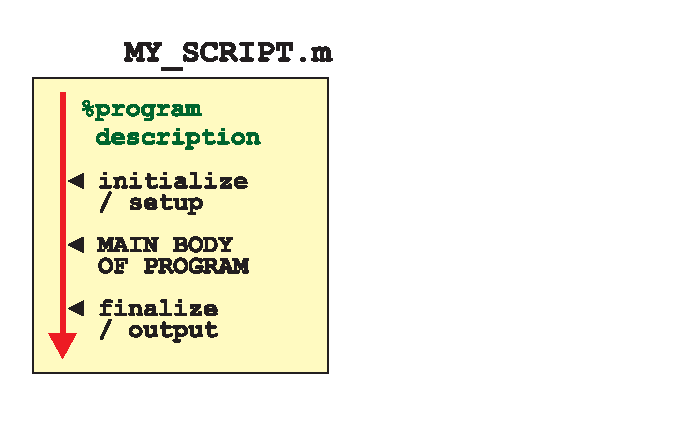
\includegraphics[width=\linewidth]{ch0-script.eps}
\caption{Schematic for a generic \textit{script}.}
\label{fig:ch0-script}
\end{marginfigure}

\begin{marginfigure}[-0.0in]
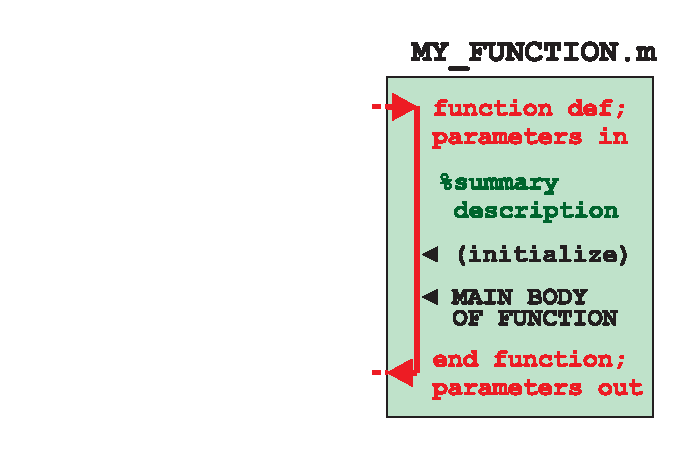
\includegraphics[width=\linewidth]{ch0-function.eps}
\caption{Schematic for a generic \textit{function}.}
\label{fig:ch0-function}
\end{marginfigure}

For the \textit{script}, the code file starts with a comment (\textcolor[rgb]{0,0.501961,0}{\texttt{\%program description}}) summarizing what the \textit{script} does, although after the \textit{function} definition header line, so to should the \textit{function} (somewhere have comment lines describing what it does).

The black left-pointing filled triangles and associated text to the right, indicate categories of code content, and occurring in what order, that the programs might contain.

The purpose of these cartoons is to help you when faced with a blank page and the question: 'Where do I start' or 'What do I write' appears prominently in your mind\sidenote[][0.0in]{Also surrounded by flashing neon lights.}. It is to give you some sort of idea what bits might go where, and what general content is required in the file. The cartoons \uline{do not} (and are not intended) to show the exact details of the code content. Nor do they necessarily indicate all the different sections needed. Conversely, not all the sections illustrated may be strictly necessary and in come examples there may be nothing to 'initalize' and there may be no constants of local parameters to define the values of at the program start.

So please -- use the cartoons as a simple visual guide to the approximate structure of your program, but \uline{do not over-interpret them}.

%------------------------------------------------

\section{'Answer' codes}

For some of the more complex codes you will be expected to write, in addition to step-by-step instructions in the text, complete 'answer' codes are be provided at the back of the text. These are provided as guides to help you structure the code as you work through the relevant section and see the 'bigger picture' of where all the parts fit together. The complete codes are obviously NOT provided for you simply to copy ... else you'll learn nothing. Except how to use the \textsf{CTRL-C} and \textsf{CTRL-V} key combinations.

Please use this provision as intended and for guidance only should you find yourself completely stuck.

%------------------------------------------------

\section{\textbf{MATLAB} versions}

The \textbf{MATLAB} software suite is constantly evolving and new and/or improved functions, and additionally functionality of the GUI, are constantly appearing. The point of this course is to provide you with a basic programming ability, as well as practical skills in applying \textbf{MATLAB} to science and data problems, rather than skill you more narrowly in the most recent \textbf{MATLAB} software version. You may well find 'easier' ways of doing things using newer \textbf{MATLAB} functions as compared to in this text, and if you do and want to utilize newer/simpler ways of doing things -- then please feel free to do so.

%----------------------------------------------------------------------------------------

\mainmatter

%----------------------------------------------------------------------------------------
% CHAPTER 1
%----------------------------------------------------------------------------------------

\chapter{Elements of ... MATLAB and data visualization}
\label{ch:01}

%------------------------------------------------

\begin{fullwidth}

\newthought{Hello Newbies!} This first lab's porpoise is to start to get you familiar with what \textbf{MATLAB} 'is' and what the heck you'd actually do with it. Specifically, you are going to learn about variables and arrays and  doing some very basic/simple math in \textbf{MATLAB}, and learn how to import and manipulate (array) data in this software environment and then do some basic plotting (aka 'data visualization'). If your are clever ... you might find menu items or buttons to click that will do the same thing as typing in boring commands at the command line. In fact, you would have to be pretty dumb not to notice all that brightly colored eye-candy in the GUI (Graphical User Interface -- i.e., menus, buttons, and stuff) at the top of  the screen. However, you will get to grips with programming much quicker if you stick with the instructions and do almost everything that is asked of you using the command line  (rather than doing stuff via the GUI ), at least to start with. You'll just have to trust me for now ... We'll start with the very basics and things that you could easily do in \textbf{Excel} instead, and build up.

\newthought{Graphics} is one of the important strengths of \textbf{MATLAB}. Although other software packages and scripting languages exist that perhaps have the edge on \textbf{MATLAB} in terms of visually appealing plots and graphs, \textbf{MATLAB} is worlds apart from e.g. \textbf{Excel}. And way way better than potato printing.

\end{fullwidth}

%------------------------------------------------

\newpage

%------------------------------------------------

\section{Using the MATLAB software}

%------------------------------------------------

\subsection{Starting MATLAB}

To start with: find the \textbf{MATLAB} icon on the desktop; run the program. You should see a number of sub-windows arranged within the main \textbf{MATLAB} window, hopefully including at the very least, the \textit{Command Window}\sidenote{Conveniently labelled \texttt{Command Window} -- you cannot possibly fail to identify it ...}. Depending on whether you have used \textbf{MATLAB} before and it has remembered your settings, windows may also include: \textit{Command History}, \textit{Workspace}, \textit{Current Folder}. If instead you see; 'Tetris', 'Grand Theft Auto: San Andreas', and 'Fortnite Battle Royale', then you have the wrong software running and are going to find learning \textbf{MATLAB} rather hard. However, there is big \$\$\$ to be made in on-line gaming tournaments these days. You could quit your degree now ...
Conversely, there are also good jobs and  \$\$\$ in being able to program. So, read on ...
\subsection{The command line\index{The command line}}

When \textbf{MATLAB} initially starts up, the \textit{Command Window}\index{Command Window} should display the following text: 

\begin{docspec}
        Academic License

>>
\end{docspec}

\noindent or nothing (the page is blank) ... or in order versions of the software:

\begin{docspec}
To get started, select MATLAB Help or Demos from the Help menu.

>>
\end{docspec}

\noindent Regardless, there should be a vertical blinking line (cursor) following the double 'greater than' symbols with an ocean of blank lines/space below\sidenote{Note that in nerd-speak the \texttt{>>} is called the command 'prompt' and is prompting you to type some input (Commands, swear words, etc.). See -- the computer is just sat there waiting for you to command it to go do something (stupid?). If one does not appear at the bottom of whatever is in the \textit{Command Window} is means that \textbf{MATLAB} is busy doing something extremely important. Or perhaps, \textbf{MATLAB} may have completely died. Either way, it will not accept any new/further commands until it is done calculating/dying.}.

If you are unfamiliar with using command-line driven software ... Don't Panic!\cite{Adams1979} Nothing bad can happen, regardless of what you do. Well, almost. It is possible to accidently clear \textbf{MATLAB}'s memory of the results of calculations and data processing and close plots and graphs before you have saved them, but \textbf{MATLAB} remembers all the commands you type, so in theory it is perfectly possible to quickly reproduce anything lost. (Later on we will be placing the sequence of commands into a file (that is saved) and so ultimately, \textbf{MATLAB} should turn out to be mostly fool-proof.)

To convince yourself that nothing dreadful will happen ... type ... anything. Actually 'anything' will do.

\begin{docspec}
\textbf{>> anything}

\textcolor{red}{Undefined function or variable 'anything'.}
\end{docspec}

Well ... not so exciting. But not so disastrous! \textbf{MATLAB} simply has no clue what you are talking about, or rather, \texttt{anything} is not a 'key word'\sidenote[][-0.25in]{i.e. a word, or sequence of characters that has a special meaning to \textbf{MATLAB} and it will act upon, as opposed to a sequence of characters that has not special meaning and \textbf{MATLAB} completely ignores.} that \textbf{MATLAB} recognises. In the specific error message, \textbf{MATLAB} could not find that \texttt{anything} was a built-in (or user-defined) \textit{function}, nor a listed \textit{variable}, both of which you'll learn about in due course.

%------------------------------------------------

\subsection{MATLAB GUI}

There are lots of fancy looking icons and pretty colors and you could spend all day staring at them and not getting any work done. Or you could learn some good programming practice. Which is why we mostly will ignore the eye-candy and little (if any) guidance will be given as to the functionality of the Graphical User Interface (\textit{GUI}). Look at this as a lesson for the user (to read the \textsf{Help}, textbook, on-line documentation, or simple go Google for an answer\sidenote{Otherwise known as Internet fishing.}).

%------------------------------------------------

\subsection{Help(!)}

If stuck at any point -- you can press the \texttt{F1} key or click on the question mark icon on the tool-bar, to bring up the indexed and searchable \textbf{MATLAB} documentation.\sidenote{It is also possible to obtain context-specific help, e.g. on a specific (built-in) \textit{function}, which we'll see in due course.}

You can also type \texttt{help} at the command line (and press the \textrm{\textsf{Return}} key).
\begin{docspec}
\textbf{>> help}
\end{docspec}

The result is perhaps not especially helpful. The typical usage is to provide the name of a \textit{function}\sidenote{Don't worry about what a \textit{function} is yet.} you require help on. Perversely, \texttt{help} is a \textit{function} and \textbf{MATLAB} provides help on \texttt{help}. The initial output to which is as follows:
\begin{docspec}
>> help \textcolor[rgb]{1,0,1}{help}

   \textbf{help} Display help text in Command Window.
\end{docspec}

In the course text, for each \textit{function} that \textbf{MATLAB} provides a comprehensive help on, such as \docenv{help}, a simple summary version will be displayed in the right hand margin in a grey box.\sidenote{Refer to the section on 'How to use this Textbook'.}

\marginnote[-0.0in]{\begin{mdframed}[backgroundcolor=light-gray, roundcorner=10pt,leftmargin=1, rightmargin=1, innerleftmargin=5, innerrightmargin=5, innertopmargin=5,innerbottommargin=5, outerlinewidth=1, linecolor=light-gray]
\docenvdef{help}
\\Typically takes a single parameter -- the name of a \textit{function}, and returns an entirely incomprehensible description of that function and its usage at the command line.
\end{mdframed}}

%------------------------------------------------

\newpage

%------------------------------------------------

\section{Basic concepts}

%------------------------------------------------

\subsection{Variables}

A \textit{variable}\index{variable} is, in a sense, a pointer to a location in computer memory where a piece of information is stored\sidenote{In the bad old days, this pointer was the actual address in memory and might have looked something like \texttt{f04da105}.}. For instance -- open up a blank worksheet in \textbf{Excel}, and in the very top left hand cell, enter the number \textsf{10}. You can see visually, that \textbf{Excel} is referencing this location as column A, and row '1'. In fact, this location ('\textsf{A1}') is indicated in the \textsf{Name Box} to the left of the \textsf{Formula Bar}.

In \textbf{MATLAB}, a variable is associated a name (rather than a letter-number code as in \textbf{Excel}) in order to make things rather more easy and convenient. The name can be almost any sequence of characters you like, regardless of whether it is a real or fake word, as long as it does not contain numbers or special characters (e.g. \#, \$, \%, ...) or spaces. So actually, you are only left with continuous sequences of characters without spaces ('words'!). Note that you can  create a variable name based on 2 (or more) real words, separated by an underscore (\texttt{\_}) if that helps describe what the \textit{variable} refers to. Valid variable names  include:

\begin{docspec}
A\\
B\\
cat\\
derpyhooves\\
this\_is\_boring\_stuff\\
BIG\\
big\sidenote{Note that \textbf{MATLAB} distinguishes between lower and UPPER case letters in a variable (i.e. \texttt{BIG} and \texttt{big} would represent two different and distinct variables). I would \uline{strongly} advise to stick to all lower case, or all upper case, to avoid possible future confusion. (or come up with a naming convention, of whatever sort (e.g. capital first letter), and stick to it.)}
\end{docspec}  

\noindent (but noting that my personal preference/recommendation is to avoid uppercase characters and stick to all lowercase)

Variables are entirely useless unless they have some information assigned to them. In fact, you can type in any of the variable names above (at the command line) and \textbf{MATLAB} will deny it knows what you are talking about\sidenote[][0.25in]{Technically, \textbf{MATLAB} reports: \texttt{Undefined function or variable} which tells you it is neither a function name (more on this later), nor is defined as having any information associated with it.}.

So far so useless -- you need to \textit{assign} something to it. (The analogous situation is that when you first open an \textbf{Excel} spreadsheet and it is completely blank -- you can still reference cell A1, but there is nothing in it.) Which brings us to quite 'what' and 'how'.

First of, you need to know that variables can have the following \textit{types} of things assigned to them:

\begin{itemize}
\setlength{\itemindent}{.2in}

\item \textbf{Integer} -- An integer number is a counting number, i.e. \texttt{1, 2, 3, ...} and including zero and negative integers.
(\textbf{MATLAB} has different representations for integer numbers, depending on how large a number you need to represent (and how much memory it will need to allocated to storing it). This is something of a throw-back to the days when computers only had 1/10000000\(^{th}\) of the memory of your iPhone and were slower than half a lemon nailed to the floor. So we will not in this text particularly worry about a numbers/computing concept called \textit{precision}.)

\item \textbf{Real (floating point)}\sidenote{The distinction (sort of) is that \textit{floating point} is a specific representation of a \textbf{real} number.} -- A \textit{real} number can have a non-integer component, e.g. 1.5 or 6.022140857 \(\times\) 10\(^{23}\). Real numbers also come in different precisions in \textbf{MATLAB} (also to do with memory allocation and speed), determining not just the number of decimal places that can be represented, but also the maximum size.
\\Be aware that you can configure\footnote{Under the menu item \textsf{Preferences} and then \textsf{Command Window}.} \textbf{MATLAB} to display a particular format for real numbers, e.g.
\\\texttt{42.0}
\\versus
\\\texttt{4.2e+01}
\\(there are identical \textit{real} numbers, just a different display format).

\item \textbf{Character} -- One or more characters, but now allowing spaces (unlike in the case of naming \textit{variables}).
Related to this is the \textbf{String} \textit{type}, which is more flexible esp. for creating arrays of characters. Which then confuses all the description in the text as a sequence of characters (or a \textit{vector} of characters) is since long-ago, known as a \textit{string}. In the text, \textit{string} will be used to refer to \textit{vector} of characters rather than the \textbf{MATLAB} \textbf{string} type. 

\item \textbf{Logical} -- a \textit{variable} that can be \texttt{true} or \texttt{false}\sidenote[][-0.5in]{As opposed to a Trump variable, that can have many different  alternative states of 'true', although generally, a Trump 'true' is in fact 'false'. An entire new branch of mathematics and logical deduction has been created just to process al this. } -- we'll come to quite what this means later.

\item \textbf{etc} -- No, not a real \textit{type}, but to note that \textbf{MATLAB} defines and recognises a whole bunch of other \textit{variable} \textit{types}, including \textbf{Complex} (\textbf{MATLAB} can handle \textit{complex numbers}) and \textbf{Object} (we will also not worry about \textit{objects}, which can incorporate a combination of types. At least, not yet ...). The \textbf{MATLAB} documentation contains a full list (and/or go Internet Fishing).

\end{itemize}

To come back to \textbf{Excel} -- if you select \textsf{Format Cells} (right-mouse-button-click over cell A1), you get to chose from a long list of 'formats', including \textsf{Number} and \textsf{Text}, and which have a loose correspondence with \textit{types} in \textbf{MATLAB}.

The next thing to learn is ... to ideally, not attempt to mix up (combine) variables of different \textit{types}. \textbf{MATLAB} is very forgiving when it comes to combining an \textit{integer} and a \textit{real} number in the same calculation, but in some other programming languages, this should be avoided.
However, even in \textbf{MATLAB}, \textit{strings} and \textit{reals} (or \textit{integers}) are very different things.\sidenote[][-3.0in]{Again -- in the \textbf{Excel} example, \textbf{Excel} will not let you add a \textbf{Number} and a \textbf{Text} value together, for instance. (Try it! You should see \textsf{\#VALUE!} reported.)} When necessary, different \textit{variable} \textit{types} can be converted between (see \textbf{Variable Type Conversion} Box).

\marginnote[-2.75in]{\begin{mdframed}[backgroundcolor=gray!10, roundcorner=10pt,leftmargin=1, rightmargin=1, innerleftmargin=5, innerrightmargin=5, innertopmargin=5,innerbottommargin=5, outerlinewidth=1, linecolor=gray!10]
\textbf{Variable Type Conversion}
\\\textbf{MATLAB} provides a variety of \textit{functions} (see later) for converting between different \textit{types} of \textit{variables}. The most commonly-used/useful ones are as follows:
\begin{enumerate}[noitemsep]
\item converting from a number to a \textit{string} (\texttt{s})
\begin{itemize}[noitemsep]
\item \texttt{s = num2str(N)}, where \texttt{N} is any number type variable
\item \texttt{s = int2str(I)}, where \texttt{I} is an integer
\end{itemize}
\item converting from a \textit{string} (\texttt{s}) to a number
\begin{itemize}[noitemsep]
\item \texttt{x = str2num(s)}, where \texttt{N} is (generally) a double precision (\textit{real}) number
\end{itemize}
\end{enumerate}
Case \#1 (\texttt{num2str}) is generally the most useful, e.g. in adding specific captions to plots (with caption text based on the value of a numerical variable) -- examples are given later.
\end{mdframed}}

The second and perhaps rather more important thing, is how to assign a value to a \textit{variable} (and in fact, create the variable in the first place). Programming languages such as \textbf{FORTRAN} require you to define the variable beforehand and assign it a \textit{type}.\sidenote{Partially true. An Alternative Fact of sorts.} \textbf{MATLAB} allows you to define and assign a value to a \textit{variable} all at the same time, and it will kindly work out the correct \textit{type} based on the value you assign to it.

You assign a value to a \textit{variable} using the \textit{assignment operator} \docenvdef{=}\sidenote{This is NOT 'equals' in \textbf{MATLAB}. Or any sane programming language. We will see the \textit{equality operator} shortly. \docenv{=} assigns the value or variable on its right, to the variable on the left.}. For example:
\begin{docspec}
A = 10
\end{docspec}
\noindent will assign the value \texttt{10} to the variable \texttt{A}. If you type this at the command line, \textbf{MATLAB} will kindly repeat what you have just told it and report the value of \texttt{A} back to you directly under the line you typed the command in at:
\begin{docspec}
A =

    10
\end{docspec}
\noindent Note that you do not need to add a space before and/or after the assignment operator (\docenv{=}). This is something of a personal programming and aesthetics preference, i.e. whether to pad things out with spaces or not. (Chose what you feel happiest with and later on, whatever leads to the fewest programming mistakes ...) i.e. 

\begin{docspec}
A = 10
\end{docspec}

\noindent is interpreted exactly the same as:

\begin{docspec}
A=10
\end{docspec}

Pause ... this is sort of fundamental (to using \textbf{MATLAB}), what you have just done here. It is the equivalent of typing '10' into the cell A1 in Excel (assuming we can equate the \textbf{Excel} location \textsf{A1} with the \textbf{MATLAB} variable \texttt{A}). In doing this, you have both: (a) created a variable \texttt{A}, and (b) assigned it a value of \texttt{10}.

\textbf{MATLAB} will also report in the \textsf{Workspace} window, the name and value, \textit{type} (unhelpfully called \textit{Class}), etc of all your current \textit{variables} (just one currently?). Actually, it is not all quite so simple. If you take a look at the \textit{Class} of the \textit{variable} \texttt{A} in the display window -- it is  listed as \textit{double} (a \textit{real} number) rather than an \textit{integer}. So by default, if \textbf{MATLAB} does not know what you really want, it defines \texttt{A} as a double precision real number\sidenote{If you genuinely wanted an integer, there are ways to do this, such as using a type conversion function form \textit{real} to \textit{integer} (see above).}.

Pausing again ... if you want to remind yourself of the \textit{variables} that you (or a program) have created -- you can refer to the \textsf{Workspace} window.\sidenote{There is a command line command for listing current variables (\texttt{whos}), but lets not bother with it.} Also listed here as noted above, is its value (and \textit{type} etc). Another way to access the value of a \textit{variable}, is to simply type in its name at the command line:

\begin{docspec}
>> A
\end{docspec}

\noindent and \textbf{MATLAB} will parrot back:

\begin{docspec}
A =

    10
\end{docspec}

The next complication comes when assigning a \textit{string} (a sequence of characters) to a \textit{variable}. For example, try:

\begin{docspec}
B = apple
\end{docspec}

\noindent and \textbf{MATLAB} is far from happy. As it turns out,  a sequence of characters  can also refer to a \textit{function}\sidenote{You will see \textit{functions} shortly. For now -- note that they are 'special' (reserved) words that perform some action and hence cannot also be used for a variable name.} in \textbf{MATLAB}, and this is what \textbf{MATLAB} looks for (i.e. a match to \texttt{apple} in the list or variable (and function) names). In other words, \textbf{MATLAB} does not know whether you intend \texttt{apple} to be a \textit{string} or a \textit{function}. It assumes \textit{function} ... but cannot find one with that name and then gives up. To delineate \texttt{apple} unambiguously as a \textit{string}, you need to encase it in (single or double) quotation marks:

\begin{docspec}
B = 'apple'
\end{docspec}

Just as \textbf{MATLAB} creates new \textit{variables} on the fly, you can re-assigned values to an existing \textit{variable}, even if this means changing the \textit{type}, e.g.

\begin{docspec}
A = 'banana'
\end{docspec}

\noindent has now replaced the real number \texttt{10} in variable \texttt{A}, with the character string \textsf{banana}. This is reflected in the updated variable list details given in the \textsf{Workspace} window (and the variable \textit{type} or \textit{Class} is now listed as \texttt{char}).\sidenote{Equally in \textbf{Excel}, you can simply type over a pre-existing value to replace it. e.g. you could type \textsf{banana} over the contents of cell \textsf{A1} (that previous held the number\textsf{ 10).}}

Finally, it is possible to suppress output to the \textsf{Command Window} when making \textit{variable} \textit{assignments} -- simply add a semi-colon (\docenvdef{;}) to the end of the \textit{assignment} statement\sidenote{Again -- your personal choice as to whether to include spaces or not between the \texttt{C},  the assignment operator \texttt{=},  the character vector \texttt{'banana'}, and \texttt{;} (Maybe try it both ways to convince yourself at least in this context, spaces do not matter.)}, i.e.

\begin{docspec}
C = 'totalbanana';
\end{docspec}

\noindent Now, nothing   is echoed back to the command line but the \textsf{Workspace} is still updated to reflect this \textit{variable} \textit{assignment}. 

%------------------------------------------------

\subsection{Numerical expressions and Arithmetic operators}

You can do normal maths in \textbf{MATLAB}. Or at least, something that looks at least a little intuitive. (In fact, I often use \textbf{MATLAB} as a calculator.)
The primary/common numerical expressions are:

\begin{itemize}[noitemsep]
\setlength{\itemindent}{.2in}
\item \docenvdef{exponentiation} --- \(^{\wedge}\) --- raises one number of variable to the power of a second, e.g. a\(^{b}\), a to the power b, which is written in \textbf{MATLAB} as \texttt{a\(^{\wedge}\)b}.
\item \docenvdef{multiplication} --- \(\times\) --- e.g. a\(\times\)b, written in \textbf{MATLAB} as \texttt{a\(\ast\)b}.
\item \docenvdef{division} --- \texttt{/} --- (written as you would expect).\sidenote{Entertainingly, it turns out that if you write the reverse, backslash character (\texttt{\textbackslash}) in the equation, you divide the over way (i.e. denominator divided by numerator).}
\item \docenvdef{addition} --- \texttt{+} --- (guess).
\item \docenvdef{subtraction} --- \texttt{-} --- again, obvious/intuitive.
\end{itemize}

Technically, these symbols are called (arithmetic) \textit{operators}.

The order in which the arithmetic \textit{operators} are written down is important and will execute them in a specific order (operators higher up the list, executed first), i.e. first \texttt{\textasciicircum}, then \texttt{\(\ast\)} and\texttt{/} (equally), and last, \texttt{+} and \texttt{-} (equally). There is also \textit{negation}, when you change the sign of a \textit{variable}, and which is executed  immediately after exponentiation. e.g. 

\begin{docspec}
B = -A
\end{docspec}

\noindent The assignment operator (\docenv{=})\sidenote{This is \textbf{NOT} 'equals to'.} comes last.

\uline{If you are unclear about the order numerical operators are carried out, then place parentheses \texttt{()} around the component of the calculation you wish to be carried out first to enforce a particular order} (this can also help in making an equation easier to read and ultimately, easier to debug code). For example, consider:

\begin{docspec}
A = 3;\\
B = 6;\\
C = 2;\\
D = C*(A/B+1)\\
E = C*A/(B+1)\\
F = C*A/B+1\\
G = A*C/B+1
\end{docspec}  

\noindent Try these out (and make up your own combinations) and confirm that the answers are what you would expect them to be.

%------------------------------------------------

\subsection{Relational and logical operators}

We will see more of \textit{relational and logical operators} later when we start to get into some proper coding. For now, you only need to know that a \textit{relational operator} is one of:

\begin{itemize}[noitemsep]
\setlength{\itemindent}{.2in}
\item \docenvdef{greater than} --- \textbf{MATLAB} symbol \(>\)
\item \docenvdef{less than} --- \textbf{MATLAB} symbol \(<\)
\item \docenvdef{greater than or equal to} --- \textbf{MATLAB} symbol \(>\)=
\item \docenvdef{less than or equal to} --- \textbf{MATLAB} symbol \(<\)=
\item \docenvdef{equality} --- \textbf{MATLAB} symbol ==
\item \docenvdef{inequality} --- \textbf{MATLAB} symbol \(\sim\)=
\end{itemize}

\noindent and  test the relationship between 2 variables.

\uline{Note that the \docenv{equality} symbol (that tests the equivalence between two variables) is represented by TWO \texttt{=} characters\texttt{ (==), }and remember that a single \texttt{=} character is the \textit{assignment operator}.}

In everyday language, the answer to any one of these relational tests would be a 'yes' or a 'no'. But in \textbf{MATLAB} (and  other computer languages), the answer is given as the binary (logical) equivalent where 'yes' is represented by \texttt{1} and 'no' by \texttt{0}. You can also use \texttt{true} (\texttt{1}) and \texttt{false} (\texttt{0}), e.g. \texttt{A = true} returns:

\begin{docspec}
A =
\\ \ \ \ \ 1
\end{docspec}  

Finally, the \textit{logical operators} (again, more on this later) are:

\begin{itemize}[noitemsep]
\setlength{\itemindent}{.2in}
\item \docenvdef{or} --- symbol \texttt{||}
\item \docenvdef{and} --- symbol \texttt{\&\&}
\item \docenvdef{not} --- symbol \texttt{\(\sim\)}
\end{itemize}

For now -- simply keep mind the existence of \textit{relational and logical operators} and what they look like and we'll look into them some more later.

%---------------------------------------------
%
\subsection{Functions (built-in)}

\textbf{MATLAB} provides numerous built-in \textit{functions}\sidenote{We will be constructing our own later, at which point it should become apparent that there is nothing particular special about them.}. These \textit{functions} have specific names assigned to them, so care needs to be take not to give a \textit{variable} the same name as a \textit{function} to avoid getting confused further down the road. Giving an exhaustive list (and brief description) is outside the scope of this text\sidenote{A full list of functions can be found in the \textbf{MATLAB} Help Documentation under \textit{functions}.}. Common \textit{functions} will be progressively introduced as this text  progress. Note that in addition to the on-line \textsf{Help} documentation, information on how to use a \textit{function} and example uses is provided by typing \texttt{help }and then the \textit{function} name (separated by a space) at the command line.

\textbf{MATLAB} also provides several built-in mathematical \textit{constants} (which save having to define a variable with the appropriate number that you no-doubt will have to look up from the internet first ...). This are simply \textit{variables} that have been already defined and assigned values, but which  you cannot change (hence the term 'constant'). For instance,  the value of \(\pi\), is assigned to a built-in \textit{function} with the name \docenvdef{pi}. You can access (display) its value  by typing its name at the command line:

\begin{docspec}
>> pi
\\ans =
\\ \ \ \ \ 3.1416
\end{docspec}  

In this example, the  use of the \textit{function} is rather trivial -- you need to tell the \textit{function} \docenv{pi} absolutely nothing, and it spits back the same thing (the value of \(\pi\)) each and every time. In most other \textit{functions}, you will  have to pass some information, and the return value will depend on that input you provide. (This ... and what exactly a \textit{function} is, will all become apparent in due course ...)  
%---------------------------------------------

\subsection{Miscellaneous commands}

Related to what you have seen so far and will see soon, some useful miscellaneous commands include:

\begin{itemize}[noitemsep]
\setlength{\itemindent}{.2in}
\item \docenvdef{clear} --- Removes all variables from the workspace.
\item \docenvdef{clear all} --- (Removes all information from the workspace.) \item \docenvdef{close} --- Closes the current figure window.
\item \docenvdef{close all} --- (Closes all figure windows.)
\item \docenvdef{exit} --- Exits \textbf{MATLAB} and hence enables an additional trip to Starbucks to be made.
\end{itemize}

Note that a useful trick -- if you want to re-use a previously used command but don't want to type it in all over again, or want to issue a command very similar to a previously-used one -- is to hit the UP arrow key until the command you want appears. This can also be edited (navigate with LEFT and RIGHT arrow keys, and use \textsf{Delete} and \textsf{Backspace} keys to get rid of characters) if needs be. Hit \textsf{Enter} to make it all happen.

For example -- try assigning a value of \texttt{2.14159} to the variable \texttt{my\_pie}. Having noted your mistake\sidenote{An 'alternative' pi?}, correct it. Do this by bring back the previous command, and editing the \texttt{2} to a \texttt{3} (and hit return). If you refer to the \textsf{Workspace} window, you can see that you have indeed successfully changed the value of \texttt{my\_pie}.\sidenote{The point is that this is much quicker than typing the entire line in again. Although later, when we start to put lines of code into files rather than typing everything at the command line, fixing mistakes becomes easier.}

Note that there is also a \textsf{Command History} window that list all the previously issued commands and allows commands to be re-run by double-clicking on them. Copy-paste and re-running of single or multiple commands is also possible.

%------------------------------------------------

\newpage

%------------------------------------------------

\section{Vectors and arrays \#1}

So far, most of your \textit{variables} have all be what are known as \textit{scalars} -- i.e. single numbers (whether \textit{real} or \textit{integer})\sidenote{An exception are when you assigned a string, which technically is a vector (assuming multiple characters in the string)}.
One of the most powerful things about \textbf{MATLAB} is its ability to represent vectors (1D columns or rows of numbers or strings) and arrays -- 2D and higher dimensional regular grids of numbers or strings. (\textit{matrix}\sidenote{Not to be confused with the film containing bad acting by Keanu Reeves.} is the name commonly given to a 2-D array.)
 
%------------------------------------------------

\subsection{Creating vectors}

\marginnote[-0.5in]{\begin{mdframed}[backgroundcolor=light-gray, roundcorner=10pt,leftmargin=1, rightmargin=1, innerleftmargin=5, innerrightmargin=5, innertopmargin=5,innerbottommargin=5, outerlinewidth=1, linecolor=light-gray]
The \docenvdef{colon operator} can be used to much more rapidy create \textit{vectors} (as long as the elements form a simple sequence in value) as compared to typing in the list of values explicitly. There are two variants to the syntax:
\begin{docspecmargin}
A = j:k
\end{docspecmargin}
and
\begin{docspecmargin}
A = j:i:k
\end{docspecmargin}
In the first example, \texttt{j} and \texttt{k} and the minimum and maximum values in the sequence of numbers in the vector. \textbf{MATLAB} completes the sequence by assuming that the values monotonically increase and that the elements are separated by one (1.0) in value. e.g. 
\begin{docspecmargin}
>> A = 0:3
\\A =
\\ \ \ \ \     0     1     2     3
\end{docspecmargin}
Note that \textbf{MATLAB} is not inclined to let you directly create a vector of elements that decrease in value (you'll need to flip this puppy about to re-order it if that is what you want -- see later).
\\In the second example, \texttt{i} is the increment \textbf{MATLAB} will use to complete the sequence from \texttt{j} to \texttt{k}. In the example in the text, you could have created the \textit{array} \texttt{B} by typing: 
\begin{docspecmargin}
>> B = 0.5:0.5:2.5
\\B =
\\ \ \ \ \     0.5000    1.0000    1.5000    2.0000    2.5000
\end{docspecmargin}
(More commonly, you might place the \textit{colon operator} and its min/(/increment)/max values inside a pair of brackets, i.e. \texttt{A = [0:3].} so that it is unambiguous that you are creating an \textit{array}
\end{mdframed}}

\textit{Vectors} are 1-D arrangements of numbers (or characters or \textit{strings}).  You can enter them into \textbf{MATLAB} as a list of space-separated value, encased in (square) brackets, \texttt{[ ]}, e.g. 

\begin{docspec}
B = [0.5 1.0 1.5 2.0 2.5]
\end{docspec}

\noindent or with the value comma-separated:
 
\begin{docspec}
B = [0.5, 1.0, 1.5, 2.0, 2.5]
\end{docspec}

Either way, you end up with a \textit{vector} on its side as a single row of numbers which in math-speak would look like:

\begin{docspec}
\(B=\)
\(\begin{pmatrix}0.5 & 1.0 & 1.5 & 2.0 & 2.5 \\
\end{pmatrix}\)
\end{docspec}

You can also create the equivalent, upright orientated \textit{vector} (as a single column of numbers) by separating the elements by a semi-colon:

\begin{docspec}
C = [0.5; 1.0; 1.5; 2.0; 2.5]
\end{docspec}

\noindent which gives the maths-speak representation:
 
\begin{docspec}
\(C=\)
\(\begin{pmatrix}0.5 \\
1.0 \\
1.5 \\
2.0 \\
2.5 \\
\end{pmatrix}\)
\end{docspec}

You might ponder on (or even try out) how you would create equivalent arrangements of numbers in an \texttt{Excel} sheet. From here on, it will rapidly become apparent why you would \uline{not} want to be doing all this in \textbf{Excel}, although it remains a presumably familiar place to start from and makes links to the weirdness of \textbf{MATLAB} from.\sidenote{As such, I encourage you to still think in \textbf{Excel} world as far as possible for a little while yet, because I think it will help get to grips with \textbf{MATLAB} array notation more quickly. And indeed, \textbf{MATLAB} has a very \textbf{Excel}-like array editor window to help bridge the gap.}

%------------------------------------------------

\subsection{Basic vector manipulation}

There are several basic and very useful ways of manipulating \textit{vectors} (and as we'll see later -- \textit{matrices}). To start with, you might want to determine the  orientation and length of a \textit{vector}. There are several different ways to go about this, which in order of grown-up-ness are:

\begin{enumerate}[noitemsep]
\setlength{\itemindent}{.2in}
\item Display the contents of the \textit{vector} in the command window by typing its name at the \textsf{command line}. Obviously, this will quickly become useless for very large \textit{vectors}\sidenote[][-1.0in]{Try creating a \textit{vector} from 1 to 100,000 and assign it to a \textit{variable}. Refer to the use of the \docenv{colon operator} (see earlier).
\\You will find that adding a semicolon to the end of the line to suppress output and instead viewing the vector in the \textsf{Workspace Window}.}. 
\vspace{1mm}
\item Refer to the \textsf{Workspace window}, -- initially, the contents of the vector are displayed (under column \textsf{Value}) and you have to count, but after a certain point, the size (and not contents) of the \textit{vector} is displayed.
\\Note that by default, the \textsf{Size} of variables is not one of the displayed columns (instead, it has to be added from \textsf{Choose Columns} right-mouse-button-click menu item)\sidenote[][-0.25in]{Although as per above -- the size is displayed under \textsf{Value} for a sufficiently large \textit{vector}.}.

\vspace{1mm}
\item Use the \docenv{length} or \docenv{size} function (see Box). 
\end{enumerate}

\marginnote[-1.0in]{\begin{mdframed}[backgroundcolor=light-gray, roundcorner=10pt,leftmargin=1, rightmargin=1, innerleftmargin=5, innerrightmargin=5, innertopmargin=5,innerbottommargin=5, outerlinewidth=1, linecolor=light-gray]
\docenvdef{length}
\\You can determine the length of a \textit{vector} A with ...
\begin{docspecmargin}
length(A)
\end{docspecmargin}
returning its \textit{integer} length, and which could in turn be assigned to a \textit{variable}, e.g. \texttt{B = length(A)}. (Technically, \docenv{length} returns the largest dimension of an \textit{array}.)
\end{mdframed}}

\marginnote[-0.0in]{\begin{mdframed}[backgroundcolor=light-gray, roundcorner=10pt,leftmargin=1, rightmargin=1, innerleftmargin=5, innerrightmargin=5, innertopmargin=5,innerbottommargin=5, outerlinewidth=1, linecolor=light-gray]
\docenvdef{size} (use \#1)
\\Returns both dimensions, even though for a \textit{vector}, one of them always has a value of \texttt{1}. This does allow you to determine its orientation though, as for the example of \texttt{A = [1:10]}: 
\begin{docspecmargin}
>> size(A)
\\ans =
\\ \ \ \ \ 1    10
\end{docspecmargin}
(1 row and 10 columns). For \texttt{A = A'}: 
\begin{docspecmargin}
>> size(A)
\\ans =
\\ \ \ \ \ 10    1
\end{docspecmargin}
(10 rows and 1 column).
\end{mdframed}}

If you find that you want a different orientation (row vs. column) of the a \textit{vector}, the \textit{vector} can be flipped around (converting row-to-column and column-to-row) using the \textit{transpose operator} (\texttt{.'}), e.g.:

\begin{docspec}
D = B.'
\end{docspec}

\noindent will turn the vector \texttt{B} into one (assigned to the \textit{variable} \texttt{D}) with the same orientation as \texttt{C}. \sidenote{Note ... \textbf{MATLAB} gives the syntax as \texttt{.'}, whereas I always only ever added the \texttt{'} bit ... which works ...}

You can also re-order the values in a \textit{vector} (hence addressing the restriction in using the \textit{colon operator} to create a \textit{vector} that the values must be monotonically increasing rather than decreasing). Depending on the orientation of the \textit{vector}, you can use either the \docenv{flipud} (for column \textit{vectors}), or \docenv{fliplr} (for row \textit{vectors}) \textit{functions} to re-order the elements (see margin box).
\marginnote[-0.0in]{\begin{mdframed}[backgroundcolor=light-gray, roundcorner=10pt,leftmargin=1, rightmargin=1, innerleftmargin=5, innerrightmargin=5, innertopmargin=5,innerbottommargin=5, outerlinewidth=1, linecolor=light-gray]
\docenvdef{flipud}, \docenvdef{fliplr}
\\These two functions allow you to re-order a vector. Their use is simple:
\begin{docspecmargin}
>> B = flipud(A)
\end{docspecmargin}
will invert the order of elements of a column vector, and:
\begin{docspecmargin}
>> B = fliplr(A)
\end{docspecmargin}
will invert the order of elements of a row vector. Simples! Lesson over.
\end{mdframed}}

%------------------------------------------------

\subsection{Addressing elements in vectors}

This next bit is maybe the single most important (and weird) part of \textbf{MATLAB} (or programming in general). As you go through this section (and also the later one on \textit{matrices}) -- it may help to have \textbf{Excel} open as a aid to visualize how \textbf{MALTAB} represents \textit{arrays} (for the  following example, you would enter the 5 numbers, from 0.5 to 2.5, in sequential cells, working down from \textsf{A1}.

In \textbf{MATLAB}, values can be extracted (or read) from a \textit{vector} by specifying the \textit{index} (technically, this should be an \textit{integer}, but \textbf{MATLAB} is pretty forgiving and you can get away with using a \textit{real} (number) when specifying an index) of the element required (counting along, left-to-right, or top-to-bottom, depending on the \textit{vector} orientation), e.g. 

\begin{docspec}
>> B(5)
\\ans =
\\ \ \ \ \ 2.5000
\end{docspec}

\noindent or:

\begin{docspec}
>> C(3)
\\ans =
\\ \ \ \ \ 1.5000
\end{docspec}

\marginnote[-2.00in]{\begin{mdframed}[backgroundcolor=light-gray, roundcorner=10pt,leftmargin=1, rightmargin=1, innerleftmargin=5, innerrightmargin=5, innertopmargin=5,innerbottommargin=5, outerlinewidth=1, linecolor=light-gray]
The \docenvdef{transpose operator}, in \textbf{MATLAB}-speak, "\textit{returns the nonconjugate transpose of A}". Who knows what that means. In slightly more everyday (i.e. down here on Earth) language, it: "interchanges the row and column index for each element". Or sort of, just interchanges the rows and columns. The operation can be written:  
\begin{docspecmargin}
>> B = A.'
\end{docspecmargin}
or  
\begin{docspecmargin}
>> B = transpose(A)
\end{docspecmargin}
In practice, you can get away with being lazy (and in fact this is how it was in the old days, and just write):  
\begin{docspecmargin}
>> B = A'
\end{docspecmargin}
(but get into the habit of using the formally correct, \textbf{Mathworks} official and UN-approved, syntax of \texttt{.'}).
\end{mdframed}}

\noindent(In this text, I will refer to accessing a particular element (or elements) of a \textit{vector} (or \textit{array}) via its \textit{index} as \textit{addressing}. Unless I forget, then I might say something else. You'll have to keep on your toes -- don't expect consistency here!)\sidenote{Recognise the parallel with \textbf{Excel} here -- the value in position \texttt{5} in the \textbf{MATLAB} vector \texttt{B}, is the same as specifying the contents of cell \textsf{A5} in \textbf{Excel}.}

There is a \textbf{MATLAB} \textit{function} \docenv{end} (see Box) that enables you to easily address (accessing via its index) the very last value in a \textit{vector} (in \textbf{MATLAB}, the \textit{index} of the first position is always \texttt{1}).

For addressing more than one element of a vector at a time, you can use the \docenv{colon operator} (see Box). \sidenote{Again -- e.g. in \textbf{Excel}, the sum of the \textsf{5} elements in column \textsf{A} (the equivalent 'vector'), would be \textsf{=SUM(A1:A5)}.}

As well as reading out an existing value of a \textit{vector}, you can also replace an existing value by assigning the new value to the appropriate \textit{index} position. e.g. to replace the first element
with a value of \texttt{0.0}:
\begin{docspec}
B(1) = 0.0
\end{docspec}

\noindent (Here, you are saying that you would like to assign the value of \texttt{0.5} to the element in the \textit{vector} given by the index \texttt{1}. The previous content of the array at \textit{index} position \texttt{1} is simply over-written.)

\marginnote[-0.50in]{\begin{mdframed}[backgroundcolor=light-gray, roundcorner=10pt,leftmargin=1, rightmargin=1, innerleftmargin=5, innerrightmargin=5, innertopmargin=5,innerbottommargin=5, outerlinewidth=1, linecolor=light-gray]
You can access more than a single element of a vector at a time, by means of the \docenv{colon operator}, \texttt{:} to define a min, max range of indices. For example:  
\begin{docspecmargin}
>> B(2:4)
\\ans =
\\   1.0000
\\   1.5000
\\   2.0000
\end{docspecmargin}
To select all elements:  
\begin{docspecmargin}
>> B(:)  
\\ans =
\\    0.5000
\\    1.0000
\\    1.5000
\\    2.0000
\\    2.5000
\end{docspecmargin}
\end{mdframed}}

\marginnote[-0.25in]{\begin{mdframed}[backgroundcolor=light-gray, roundcorner=10pt,leftmargin=1, rightmargin=1, innerleftmargin=5, innerrightmargin=5, innertopmargin=5,innerbottommargin=5, outerlinewidth=1, linecolor=light-gray]
\docenvdef{end}
\\Represents the largest index in a \textit{vector} when addressing it, or in \textbf{MATLAB}-speak: "end can ... serve as the last index in an indexing expression".
\end{mdframed}}

%------------------------------------------------

\newpage

%------------------------------------------------

\section{Basic graphing (aka. 'data visualization')}

So far ... I suspect this is heavy-going and there is a lot to try and remember, such as command names, although knowing just that certain commands exist, is enough to start with and \textbf{MATLAB} \textsf{Help} can be used later to find out the exact name (and usage syntax). All this, and we have not  even  gotten on to \textit{matrices} (2-D arrays) yet ... So, we'll take a diversion to look at some basic plotting techniques that will  make sense now that you can create \textit{vectors} of numbers to plot (and later, important some 'real' data). Unless you have forgotten how to create \textit{vectors} already ... :(

%------------------------------------------------

\subsection{Plotting}

First -- create yourself a dummy dataset to plot. You are going to need to create yourself a pair of \textit{vectors} -- these can have any values in them that you like, but perhaps aim for 1 vector with values counting up from 1 to 10 (or similar) -- this will form your \textit{x}-axis, and the 2nd column ... whatever you like. \sidenote[][-3.00in]{Looking ahead -- you could create a y-axis \textit{vector} formed of the squares of the numbers in the x-axis \textit{vector}: 
\begin{docspecmargin}
>> Y = X.\(^{\wedge}\)2  
\end{docspecmargin}
(The \texttt{.\(^{\wedge}\)} bit says to square the value of each and every  element in the \textit{vector}.)}
The command \docenvdef{figure} creates a \textsf{figure window}, which is where \textbf{MATLAB} displays its graphical output ... but on its own, without anything in it ... useless. So, lets put something in it, with the simplest possible graphical way of displaying data called \docenv{plot}. 

\marginnote[-2.25in]{\begin{mdframed}[backgroundcolor=light-gray, roundcorner=10pt,leftmargin=1, rightmargin=1, innerleftmargin=5, innerrightmargin=5, innertopmargin=5,innerbottommargin=5, outerlinewidth=1, linecolor=light-gray]
\docenvdef{plot}
\\The \textbf{MATLAB} function \docenv{plot} ... plots. More specifically, it plots pairs of (x,y) data and by default, does not plot the points explicitly but joins the(x,y) locations up by straight line segments. \textbf{MATLAB} calls these a '2D line plot', although there are plotting options that allow you only to display the individual (x,y) points (making it like the \docenv{scatter} function, which we'll see later).
\\Its most basic usage is: 
\begin{docspecmargin}
plot(X,Y)
\end{docspecmargin}
where \texttt{X} and \texttt{Y} are vectors -- of the same length (\uline{important}), but not necessarily of the same orientation (i.e. if one was a row vector and one a column vector, \textbf{MATLAB} would work it out, although it is perhaps best to avoid such a situation arising).
\\There are many options that go with this function, some of which we'll see and use later. You can also input matrixes as \texttt{X} and \texttt{Y} apparently. But I have absolutely no clue as to what might happen. I suspect that the plot will end up looking like a bad acid trip. 
\end{mdframed}}

With any new \textbf{MATLAB} command (\textit{function}), get into the habit of looking up the \textsf{help} text  (also refer to alternative/simplified help provided in this text). The key information that will get you started appears at the very top of the text that \textsf{help} returns on \texttt{plot}:

\begin{docspec}
PLOT(X,Y) plots vector Y versus vector X.
\end{docspec}

\noindent This tells you that you need to 'pass' to \texttt{plot}, your \textit{x}-axis data \textit{vector} (by its variable name), followed by your y-axis data \textit{vector} (by its variable name), with the 2 variable names comma separated:

\begin{docspec}
\textbf{>> PLOT(X,Y)};
\end{docspec}


 Do this, and depending on just what or how random your \textit{y}-axis data was, you should end up with something like Figure \ref{fig:plot-basic} in a window captioned "\texttt{Figure 1}".\sidenote{If you cannot see the figure window ... check that the window is not hidden behind the main \textbf{MATLAB} program window!} 

This ... is easily the least professional plot ever (aside from anything created in \textbf{Excel}). And one that breaks all the most basic rules of scientific presentation, such as an absence of any labelling of axes. There is also no title, although here in the course text I have added a figure caption in the document so I can sort of get away with it. This is the default output of the basic \texttt{plot} function and you'll just have to deal with it (i.e. add a series of commands to add missing elements of the \texttt{plot}).

\begin{marginfigure}[0.0in]
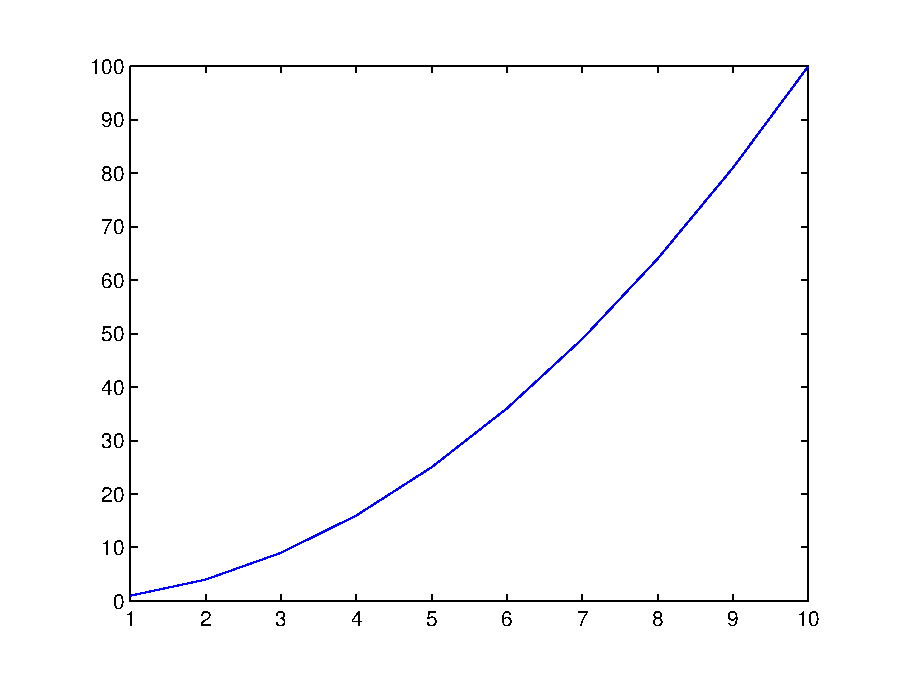
\includegraphics[width=\linewidth]{ch1-plot-basic1.eps}
\caption{Example of the default output of the \texttt{plot} function.}
\label{fig:plot-basic}
\end{marginfigure}

Note that by default, \textbf{MATLAB} also scales both axes to reasonably closely match the range of values in the two data vectors. In the example here, the default min and max
axes limits in fact turn out to be the min and max values in the \textit{x} and y-axis data because the data is composed of relatively simply/whole numbers. If however the maximum \textit{y} value was very  slightly larger, you'd see that \textbf{MATLAB} would adjust the maximum \textit{y}-axis limit to the next convenient value so as to preserve a relatively simple series of labelled tick marks in the axis scale. In fact, why not try that -- replace your maximum data value\sidenote[][-1.25in]{Remember that you can replace e.g. the last element of \textit{vector} \texttt{Y} with the value \texttt{9.9}, by:
\begin{docspecmargin}
Y(end) = 9.9;
\end{docspecmargin}}, with a value that is very slightly larger (an example is given in Figure \ref{fig:ch1-plot-basic3}).
\sidenote[][-0.75in]{If you have created a dummy dataset in which the value in the last row is the largest, replacing it is simple -- remember the use of \texttt{end} in addressing an element in an array. If your dataset does not monotonically increase and the largest value falls somewhere in the middle ... you could cheat' and open the array in the variable editor and discover which row it occurs on.} Then re-plot and note how it has changed (if at all -- it will depend somewhat on what data you invented in the first place).

\begin{marginfigure}[0.0in]
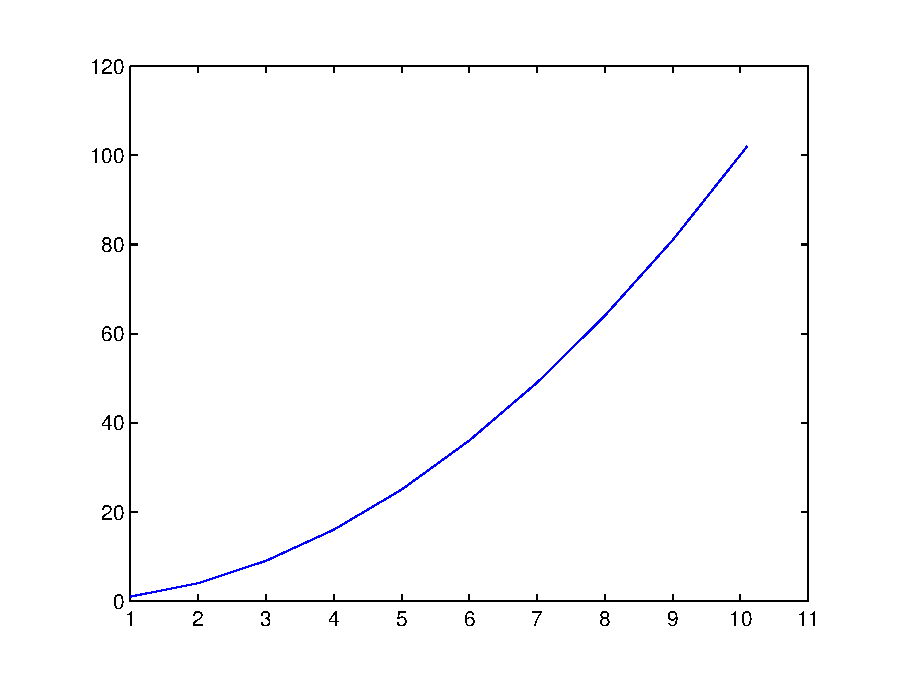
\includegraphics[width=\linewidth]{ch1-plot-basic3.eps}
\caption{A plot illustrating axis auto-scaling (maximum \textit{x} and \textit{y} values now slightly larger than 10 and 100, respectively).}
\label{fig:ch1-plot-basic3}
\end{marginfigure}

%------------------------------------------------

\subsection{Graph labelling}

You have two options for editing the figure and e.g. adding axis labels. Firstly, you can use the \textit{GUI} and the series of menu items and icons at the top of the \textsf{Figure window} to manipulate the figure. I suspect you'll prefer this ... but it is not very flexible, or rather, it requires your input each and every time you want to make changes or additions to a figure. The second possibility is to issue a series of \textbf{MATLAB} commands at the \textsf{command line}. (The advantage with the latter we'll see later when we introduce \docenvdef{m-files}.) For now, I'll illustrate a few basic commands:

\begin{marginfigure}[0.0in]
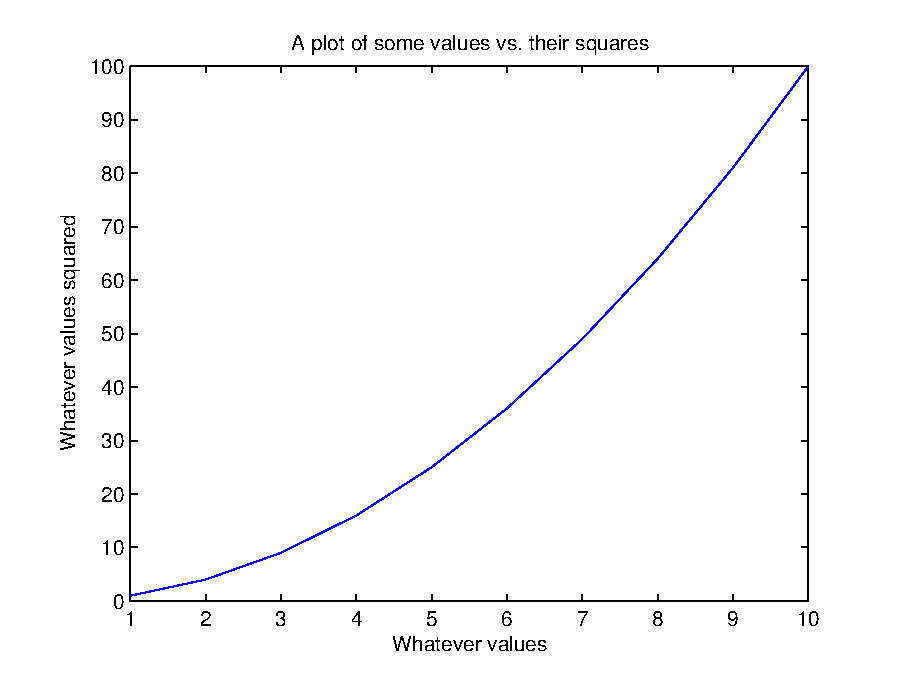
\includegraphics[width=\linewidth]{ch1-plot-basic2.eps}
\caption{A (only very slightly) improved plot.}
\label{fig:ch1-plot-basic2}
\end{marginfigure}

\begin{enumerate}[noitemsep]
\setlength{\itemindent}{.2in}
\item The first, obvious thing to do is to add axis labels. The commands are simple -- \docenvdef{xlabel} and \docenvdef{ylabel}. They each take a string as an input, which is the text you would like to appear on the axis (see Box).
If you change your mind, simply re-issue the command with the text you would like instead.
\vspace{1mm}
\item The command for title, perhaps unsurprisingly, is \docenvdef{title} (also see Box). Again, pass the text you would like to appear as a string (in inverted commas \texttt{' '}), or pass a the name of variable that contains a string (no \texttt{'}' is then needed).
\vspace{1mm}
\item You might want to specify the axis limits. The command is \docenv{axis} (see Box) and it takes a vector of 4 values as its input -- in order: minimum x, maximum x, minimum y, and maximum y value. e.g. \texttt{axis([0 10 -100 100])} would specify an \textit{x}-axis running from 0 to 10, and a \textit{y}-axis from -100 to 100.
\end{enumerate}

Information as to how to use all of these commands can be found via \textbf{MATLAB} \texttt{help}. 

Employing the above 3 suggestions gives rise to the improved plot shown in Figure \ref{fig:ch1-plot-basic2}, is given in the margin.

\marginnote[-1.5in]{\begin{mdframed}[backgroundcolor=light-gray, roundcorner=10pt,leftmargin=1, rightmargin=1, innerleftmargin=5, innerrightmargin=5, innertopmargin=5,innerbottommargin=5, outerlinewidth=1, linecolor=light-gray]
Example of adding axis labels and a plot title ...
\begin{docspecmargin}
>> xlabel ... 
\\ \ \ ('Whatever values');
\\>> ylabel ...
\\ \ \ ('Values squared');
\\>> title ...
\\ \ \ ('A plot of some ...
\\ \ \ values vs the ... 
\\ \ \ squares');   
\end{docspecmargin}
(The notation gets confusing in a narrow box like this -- the\texttt{ ...} indicates that the line should be \uline{continuous} and not broken across 2 different lines.)
\end{mdframed}}

Note that in the usage of all the above listed commands, they all require something to be passed within a set of parentheses -- \texttt{( )}. In fact, they are all \textbf{MATLAB} \textit{functions} and require an input (hence the use of the parentheses). Some of the functions require a \textit{string} input, such as the name of the title in \docenv{title}, and this must be encased in quotation marks -- \texttt{' '} to designate it a string rather than a \textit{variable} name.\sidenote[][-0.5in]{You could instead assign a \textit{string} to a \textit{variable}, and then pass the \textit{variable} name (no quotation marks).} This will all become clearer once you start creating your own \textit{functions} (computer programs) in the next chapter.

%------------------------------------------------

\subsection{Sub-plots}

You can also have more than one plot in a single \textsf{Figure window}. As an example, create some sine waves using the \docenvdef{sin} function (see \texttt{help}) over the range 0 < \textit{x} < 2\(\pi\), e.g.:
\begin{docspec}
\textbf{>> x = 0:0.1:2*pi;
\\>> y = sin(x);
\\>> y2 = sin(2*x);}
\end{docspec}
(Note how in the first line, the \textit{colon operator} is used to create an \textit{x} vector from 0 to 2\(\pi\), in steps of 0.1. The second and third lines calculate the sine of all the x values, and sine of 2 times the \textit{x} values, respectively, and assign the results to a pair of new vectors, \texttt{y} and \texttt{y2}.)

\marginnote[-3.0in]{\begin{mdframed}[backgroundcolor=gray!10, roundcorner=10pt,leftmargin=1, rightmargin=1, innerleftmargin=5, innerrightmargin=5, innertopmargin=5,innerbottommargin=5, outerlinewidth=1, linecolor=light-gray]
\docenvdef{axis}
\\For once, helpfully, \textbf{MATLAB} says:
\\"\textit{\texttt{axis([xmin xmax ymin ymax])} sets the limits for the x- and y-axis of the current axes.}"
\\\noindent which is about all you need to know (other than the minimum and maximum limits along the \textit{x-axis} are represented by \texttt{xmin}, \texttt{xmax}, and the minimum and maximum limits along the \textit{y-axis} are \texttt{ymin}, \texttt{ymax}).
Simply stick to the format, with a vector of 4 values (remembering the square bracket notation \texttt{[]}), inside of \texttt{axis()}, and you should not go wrong!
\\For example, to scale the plot with the x-axis going from 0-10, and the y-axis from -100-100, you would type:
\begin{docspecmargin}
axis([0 10 -100 100]); 
\end{docspecmargin}
\end{mdframed}}

To place several different plots on the same figure uses the \docenvdef{subplot} command \sidenote{>> help subplot}. The \docenv{subplot} command is used as: \texttt{subplot(m,n,p)} where \texttt{m} is the number of rows of plots you want to have in your figure, \texttt{n} is the number of columns of plots in your figure, and \texttt{p} is the index of the plot you wish to create (see: Figure \ref{fig:ch1-subplot}).  

\begin{marginfigure}[0.0in]
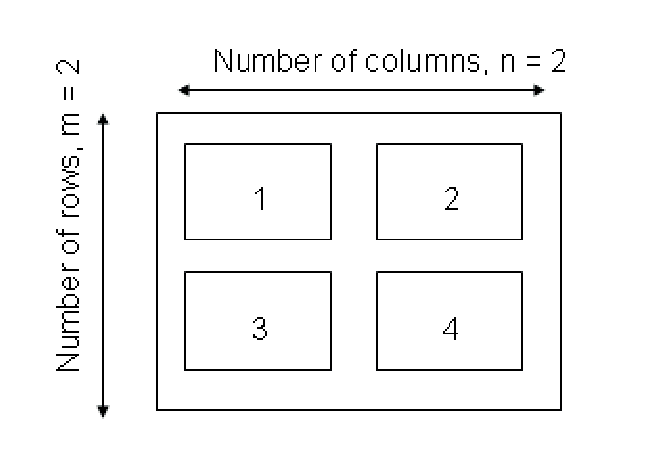
\includegraphics[width=\linewidth]{ch1-subplot.eps}
\caption{Arrangement of subplots.}
\label{fig:ch1-subplot}
\end{marginfigure} 

The basic code then goes something like:
\begin{docspec}
>> figure(1);
\\>> subplot(2,2,1);
\\>> plot(x,y);
\\>> subplot(2,2,2);
\\>> plot(x,y2);
\\>> subplot(2,2,3);
\\>> plot(x,-y);
\\>> subplot(2,2,4);
\\>> plot(x,-y2);
\end{docspec}

\noindent In this case, the 3rd and 4th subplots simply display the inverse of the curves in the subplots above. 

%------------------------------------------------

\subsection{Saving graphics and figures}

You might just want to save the figure. (Why create it in the first place in fact if you are just going to throw it away ... ?) Again, you can do this via the \textit{GUI} or at the \textit{command line}
\sidenote[][-0.0in]{
To export a graphic at the command line, use the \docenvdef{print} function. To cut a long story short (see: \texttt{help print}), to print to a postscript file:
\\\texttt{print('-dpsc2', FILENAME)}
\\\noindent where \texttt{FILENAME} is the filename as a \textit{string} or a \textit{variable} containing a \textit{string}.
}.
From the \textit{GUI}, you have the option to save the figure in a way that can be loaded later and re-edited -- this is the \texttt{.fig} format option. Or you can save (export) in a variety of common graphics formats (although once saved in this format, the graphics can only be edited later using a graphics package).

You can also close \textsf{figure windows} (see Box). No seriously. They are not forever. ;)

\marginnote[-0.50in]{\begin{mdframed}[backgroundcolor=light-gray, roundcorner=10pt,leftmargin=1, rightmargin=1, innerleftmargin=5, innerrightmargin=5, innertopmargin=5,innerbottommargin=5, outerlinewidth=1, linecolor=light-gray]
To close the current (active) \textsf{Figure window}, the command is:
\\ \texttt{>> close}
\\ \noindent To close all currently open \textsf{Figure windows}:
\\ \texttt{>> close all}
\end{mdframed}}

%------------------------------------------------

\newpage

%------------------------------------------------

\section{Vectors and arrays \#2}

A \textit{matrix} is another special case of an \textit{array} -- this time 2-D (rather than 1-D in the case of a vector). \textbf{MATLAB} totally hearts them.
 
\subsection{Creating matrices and arrays}

You can enter \textit{matrices} (2-D arrays) into \textbf{MATLAB} in several different ways:

\begin{enumerate}[noitemsep]
\setlength{\itemindent}{.2in}
\item Enter an explicit list of elements.
To enter the elements of a \textit{matrix}, there are only a few basic conventions:
\begin{itemize}[noitemsep]
\setlength{\itemindent}{.4in}
\item Separate the elements of a row with blanks or commas.
\item Use a semicolon, \texttt{;} , to indicate the end of each row.
\item Surround the entire list of elements with  brackets, \texttt{[ ]}.
\end{itemize}
\item Load matrices from external data files.
\item Generate matrices using built-in functions.
\end{enumerate}

\newthought{As an example}, type in the following at the command prompt:
\begin{docspec}
\textbf{A = [15 7 11 6; 13 1 6 10; 21 17 5 3; 5 15 20 9]}
\end{docspec}
\noindent \textbf{MATLAB} then displays the matrix you just entered\sidenote{Remember that you can add an \texttt{;} to the end of the line to prevent the results of the \textit{variable} assignment being displayed in the \textsf{Command Window}.}:
\begin{docspec}
A =\\
\ \ \ \ 15   7  11   6\\
\ \ \ \ 13   1   6  10\\
\ \ \ \ 21  17   5   3\\
\ \ \ \ 5   15  20   9
\end{docspec}

In math-speak, this would be equivalent to:

\vspace{2mm}
\(A=\begin{pmatrix}15 & 7 & 11 & 6 \\
13 & 1 & 6 & 10 \\
21 & 17 & 5 & 3 \\
5 & 15 & 20 & 9 \\
\end{pmatrix}\)
\vspace{2mm}

\noindent Once you have entered the \textit{matrix}, it is automatically remembered in the \textbf{MATLAB} workspace. You can refer to it simply as \texttt{A}.

Now go find the \textit{array} you have just created in the \textsf{Workspace window}. Double-click on its name icon and see what goodies appear on the screen. This is a fancy \textit{array} editor which looks a bit like one of those dreadful \textbf{Excel} spreadsheet things. You can see that this might be handy to edit, view, and keep track of at least moderate quantities of data. This is a useful facility to have. However, we are going to concentrate on the command-line operation of \textbf{MATLAB} in this class because that will give you far more power and flexibility in applying numerical techniques to problem solving, and will form the basis of \textit{scripting} (computer programming by another name) that we will see in a few lectures time. Close down this nice toy to leave just the original windows.

Elements in the \textit{matrix} can be addressed using the syntax:
\begin{docspec}
A(i,j)
\end{docspec}
where \uline{\texttt{i} is the row number, and \texttt{j} is the column number.} It is very very easy to keep forgetting in which order the rows and columns are indexed, but I'll tell you here and now before I forget:
\hfill \break
\\{\LARGE rows, columns}
\hfill \break
\\\noindent(You can always create a test \textit{matrix} and access a specific element to check if in doubt!)
In the example above:
\begin{docspec}
>> A(1,3)
\\ans =
\\ \ \ \ \ 11
\end{docspec}
\noindent (i.e. the value of the element in the 1st row, 3rd column, is \texttt{11}).

In general, the same \textit{functions} and \textit{operators} that applied to \textit{vectors} and you saw earlier, also apply to \textit{matrixes} (or specific dimensions of matrices).

\marginnote[-0.0in]{\begin{mdframed}[backgroundcolor=light-gray, roundcorner=10pt,leftmargin=1, rightmargin=1, innerleftmargin=5, innerrightmargin=5, innertopmargin=5,innerbottommargin=5, outerlinewidth=1, linecolor=light-gray]
Similarly as for vectors, you can access more than a single element of a matrix by means of the \docenv{colon operator}, \texttt{:}. For example: \\\texttt{A(:,1)} -- selects the 1st column
\\\texttt{A(3,:)} -- selects the 3rd row
\\\texttt{A(2:3,2:3)} -- selects the 2\(\times\)2 matrix of values lying in the centre of \texttt{A}, while \texttt{A(1:2,:)} selects the top half (first 2 rows) of the matrix.
\end{mdframed}}

Finally -- a fundamental way of accessing data that you need to learn and be familiar with, is to employ the \textit{colon operator} to select specific columns (or rows) of data. You'll find that this skill  ends up inherent to many of your attempts to process and graph data. For instance, if your (\textit{x},\textit{y}) data to plot ended up in \textbf{MATLAB} workspace in matrix form (it very commonly does) rather than as 2 sperate vectors (as you had when you first plotted anything), you will need to select separately the \textit{x} (e.g. 1st column) data, and the \textit{y} (2nd column) data, and pass these to the \texttt{plot} function.
For the example of matrix A above, all the first column data can be selected by typing \texttt{A(:,1)}\sidenote{Remembering the HUGE hint above in 100 pt font as to the order of rows and columns ...}, which says all the rows (\texttt{:}) in the first column. Similarly, all the 2nd column data alone can be selected by \texttt{A(:,2)}. (You'll practice this endlessly later on and hopefully get it!)


\marginnote[-0.25in]{\begin{mdframed}[backgroundcolor=light-gray, roundcorner=10pt,leftmargin=1, rightmargin=1, innerleftmargin=5, innerrightmargin=5, innertopmargin=5,innerbottommargin=5, outerlinewidth=1, linecolor=light-gray]
You can also determine the shape of your \textit{array} using the \docenvdef{size} function. For a 2D \textit{array} (\textit{matrix}), when you pass it the name of your array, it returns the number of rows followed by the number of columns (in that order). 
\end{mdframed}}

%------------------------------------------------

\subsection{Basic matrix manipulation}

You can treat \textit{vectors} and \textit{matrices} (or parts of \textit{vectors} and \textit{matrices}), mathematically, as you would treat single values (i.e. \textit{scalars}) but unlike a \textit{scalar}, the transformation is applied to all specified elements of the \textit{array}. This applies for all the basic \textit{arithmetic operators}\sidenote{Technically ... or at least to be consistent with other operations, you might write multiplication as \texttt{.*} rather than just plain old \texttt{*}. The preceding dot tells \textbf{MATLAB} not to treat this as matrix multiplication but to carry out the operation on each element in turn. In this case, it is the same thing (and both notations work the same), but later, is not. (This will make more sense when you get to see it in action, later.)}. For example, for \textit{vector} \texttt{B} in the earlier example,
\begin{docspec}
>> 2*B
\\ans =
\\ \ \ \ \ 0     2     3     4     5
\end{docspec}
and
\begin{docspec}
>> B-1.5
\\ans =
\\ \ \ \ \ -1.5000   -0.5000         0    0.5000    1.0000
\end{docspec}

\vspace{1mm}
\noindent\rule{4cm}{0.5pt}
\vspace{2mm}

\noindent In the following, having previously created the matrix \texttt{A}, you will derive a matrix \texttt{C}, and then preform some operations on it. to start with: multiply all the elements of \texttt{A} by the number \texttt{17}. Assign the answer to a 3rd array (\texttt{C}). 

\newthought{Question:} What is the value of the element \texttt{C(2,3)}? How would you ask for the 4th row, 2nd column element of the array \texttt{C}, and what is its value?

\newthought{Question:} What is the sum of the 4th column of \texttt{C}
\marginnote[-0.75in]{\begin{mdframed}[backgroundcolor=light-gray, roundcorner=10pt,leftmargin=1, rightmargin=1, innerleftmargin=5, innerrightmargin=5, innertopmargin=5,innerbottommargin=5, outerlinewidth=1, linecolor=light-gray]
The \textit{function} \docenvdef{sum} ... sums things. The \textbf{MATLAB} Help documentation (\texttt{help sum}) says:
\\'\texttt{If A is a vector, sum(A) returns the sum of the elements.}'
\\'\texttt{If A is a matrix, sum(A) treats the columns of A as vectors, returning a row vector of the sums of each column.}'
\end{mdframed}}
? (Sure -- you also do it by using a calculator, but you will not always have such a small data-set as here. Perhaps you'll get a much larger data-set in an assessed exercise ;) So, practice doing it properly.) The \textbf{MATLAB} function for this is \docenv{sum}.

\newthought{Question:} What is the sum of the 2nd row of \texttt{C}?
 For a \textit{matrix} (rather than a \textit{vector}) as input, \docenv{sum}  returns the individual sums of each column, and so on its own;
\begin{docspec}
>> C\\
C =\\
\ \ \ \ 255   119   187   102\\
\ \ \ \ 221    17   102   170\\
\ \ \ \ 357   289    85    51\\
\ \ \ \ 85   255   340   153\\
\vspace{2mm}

>> sum(C)\\
ans =\\
\ \ \ \ 918   680   714   476\\
\end{docspec}
\noindent gives you a row \textit{vector} consisting of the sums of the individual columns of the \textit{matrix} \texttt{C} above.

This is where the \docenv{transpose} function (\texttt{'}) comes in handy (see earlier). In this case, it flips a (2D) \textit{matrix} around its leading diagonal (columns become rows, and rows, columns)\sidenote[][-1.0in]{This is almost true. Technically the function you want is \texttt{.'}, as \texttt{'} will change the sign of any imaginary components. For real numbers, they are the same.}
\marginnote{\begin{mdframed}[backgroundcolor=light-gray, roundcorner=10pt,leftmargin=1, rightmargin=1, innerleftmargin=5, innerrightmargin=5, innertopmargin=5,innerbottommargin=5, outerlinewidth=1, linecolor=light-gray]
In addition to \docenv{transpose}, other useful array manipulation functions include:
\\\noindent \docenv{flipup} -- flips the matrix in the up/down direction
\\\noindent \docenv{fliplr} -- flips the matrix in the left/right direction
\\\noindent \docenvdef{rotate} -- rotates the matrix
\\\noindent(As always, refer to the \texttt{help} on specific functions.)
\end{mdframed}}.
\begin{docspec}
>> C'\\
ans =\\
\ \ \ \ 255   221   357    85\\
\ \ \ \ 119    17   289   255\\
\ \ \ \ 187   102    85   340\\
\ \ \ \ 102   170    51   153
\end{docspec}
\noindent (transposing the \textit{matrix} turns the rows into columns)
\begin{docspec}
>> sum(C')\\
ans =\\
\ \ \ \ 663   510   782   833
\end{docspec}
\noindent Now you get a row \textit{vector} consisting of the sums of the individual columns of the \textit{matrix} C, but since you have transposed the \textit{matrix} \texttt{C} first, these four values are actually equal to the row sums.

Finally, you could transpose the answer:
\begin{docspec}
>> sum(C')'\\
ans = \\
\ \ \ \ 663\\
\ \ \ \ 510\\
\ \ \ \ 782\\
\ \ \ \ 833
\end{docspec}
\noindent to give you  a row \textit{vector} format that corresponds to the rows  of the original \textit{matrix} \texttt{C}.
\sidenote[][-0.25in]{Note how you can combine multiple \textit{functions} in the same statement to create \texttt{sum(C')'}. However, to start with, it is much safer to do each step separately and hence be sure what you are doing.}

More recent versions of \textbf{MATLAB} let you calculate sums of rows more easily, by being able to specify the dimension that you sum across. e.g. in the original example:
\begin{docspec}
>> C\\
C =\\
\ \ \ \ 255   119   187   102\\
\ \ \ \ 221    17   102   170\\
\ \ \ \ 357   289    85    51\\
\ \ \ \ 85   255   340   153\\
\vspace{2mm}
\end{docspec}
To sum the columns:
\begin{docspec}
>> sum(C,1)\\
ans =\\
\ \ \ \ 918   680   714   476\\
\end{docspec}
and then to sum the rows:
\begin{docspec}
>> sum(C,2)\\
ans =\\
ans = \\
\ \ \ \ 663\\
\ \ \ \ 510\\
\ \ \ \ 782\\
\ \ \ \ 833
\end{docspec}


\newthought{Question:} What is the sum of *all* the elements in the \textit{matrix} \texttt{C}?

You could sum all the columns to give you a row \textit{vector} of partial sums, and then sum the elements in the row \textit{vector} to give you the grant total sum of all the elements. You can do this, either in completely separate steps\sidenote{In general in programming -- use as many smaller, separate steps as you like and are most comfortable. The more you break down the calculation, the clearer it will be to you and the easier to debug if things go wrong. However, this does come at the expense of longer and longer code and sometimes more compact code is easier to deal with.}:
\begin{docspec}
>> D = sum(C);\\
>> E = sum(D);
\end{docspec}
or all in one go:
\begin{docspec}
>> F = sum(sum(C));
\end{docspec}

It does not matter if you sum the column of \texttt{C} first, or the row first -- maybe test this to satisfy yourself that this is true.

More recent \textbf{MATLAB} versions also give you a short-cut:
\begin{docspec}
>> sum(C,'all')\\
ans = \\
\ \ \ \ 2788\\
\end{docspec}

%------------------------------------------------

\subsection{Some matrix math :(}

We will not concern ourselves overly with multiplying \textit{vectors} and \textit{matrices} together ... but you should be aware that \textbf{MATLAB} can do matrix math. For now, it is worth nothing the difference between \texttt{*} and \texttt{.*} operators in the context of arrays. For example, consider 2 vectors, \texttt{A} and \texttt{B}:

\begin{docspec}
>> A = [1 1 2 2];\\
>> B = [1 2 3 4];
\end{docspec}

To multiple the elements of \texttt{A} and \texttt{B} together \uline{pair-wise}, use .*:

\begin{docspec}
>> C = A.*B
\\
C =\\
\ \ \ \ 1     2     6     8
\end{docspec}

Without the dot, you get the vector product ... well, you would if the \textit{vectors} were in an appropriate orientation, i.e.:

\vspace{1mm}
\(\begin{pmatrix}1 & 1 & 2 & 2 \\
\end{pmatrix}\times\begin{pmatrix}1 \\
2 \\
3 \\
4 \\
\end{pmatrix}\)
\vspace{1mm}

\noindent which you get by typing:

\begin{docspec}
>> C = A*B'
\\
C =\\
\ \ \ \ 17
\end{docspec}
(which is  calculated from: \(1\times1 + 1\times2 + 2\times3 + 2\times4\)).

An example of the equivalent matrix usage is:

\begin{docspec}
>> D = [1 1; 2 2];\\
>> E = [1 2; 3 4];
\end{docspec}

The pair-wise multiplication of each element of the 1st matrix with the corresponding element of the 2nd matrix is:
\begin{docspec}
>> F = E.*E
\\
F =\\
\ \ \ \ 1     4\\
\ \ \ \ 9    16
\end{docspec}

In contrast, for matrix multiplication, written in math-speak as:

\vspace{2mm}
\(\begin{pmatrix}1 & 1 \\
2 & 2 \\
\end{pmatrix}\times\begin{pmatrix}1 & 2 \\
3 & 4 \\
\end{pmatrix}\)
\vspace{2mm}

we would write:

\begin{docspec}
>> F = E*E
\\
F =\\
\ \ \ \  7    10\\
\ \ \ \ 15    22
\end{docspec}

If your matrix math is rusty and you are not following this, maybe refresh it (your memory of basic matrix math).

%------------------------------------------------

\newpage

%------------------------------------------------

\section{Loading and saving data}

There are a number of different ways to load/import data into the \textbf{MATLAB} \textsf{Workspace}. Rather than try and tediously list and describe the commands and syntax and blah blah, we'll be going through a couple of (hopefully) slightly less tedious data-based examples as we progress through the course text. In this way, if nothing else, you might accidently learn some science even if nothing much about \textbf{MATLAB} ...

%------------------------------------------------

\subsection{Where am I?}

Before anything -- you need to know 'where you are'. If the file you want to load in, is not in the directory \textbf{MATLAB} is using, it will not find it. And if you save something and have no idea where it is being saved ... that can hardly go well.

\textbf{MATLAB} has a default directory that it starts up in and looks at first. For basic Windoz installations\sidenote[][-1.0in]{At installation, this directory can be specified and hence may not be this one. Also -- different operating systems will have different default locations.} of the software, this directory is:

\begin{docspec}
C:\textbackslash Users\textbackslash mushroom\textbackslash Documents\textbackslash MATLAB
\end{docspec}

You can determine which directory \textbf{MATLAB} is currently 'in', either at the command line:

\begin{docspec}
> cd
\end{docspec}

\noindent or it should be displayed in a toolbar above the \textsf{Command Window}. 

It is unlikely that you want to have to save all your files here. More likely, you may have a course folder somewhere, possibly with sub-folders for each week (or whatever), so you will need to change the \textbf{MATLAB} directory that you are working in, to match the one where your files are. 

Easiest ... is to use the GUI -- the toolbar above the \textsf{Command Window} can be used to change the current (working) folder. The contents of the current folder are automatically displayed in the \textsf{Current Folder} pane on the left. (If the \textsf{Current Folder} pane is not present in your \textbf{MATLAB} layout, it can be selected form the \textsf{Layout} drop-down menu.)

You can also do this at the the command line ... which is much less fun and you are less likely to need to do it this way. The instructions are included below for completeness ... but you can skip over them if you wish
\sidenote[][-0.0in]{Just remember that there are ways of navigating around your computer storage via the command line.} ...

\marginnote[-1.0in]{\begin{mdframed}[backgroundcolor=light-gray, roundcorner=10pt,leftmargin=1, rightmargin=1, innerleftmargin=5, innerrightmargin=5, innertopmargin=5,innerbottommargin=5, outerlinewidth=1, linecolor=light-gray]{
\docenvdef{addpath}
\\The command \docenv{addpath} will add a search path to the \textbf{MATLAB} workspace. The syntax is:
\\\texttt{addpath(DIRECTORY\_PATH)}
\\where \texttt{DIRECTORY\_PATH} is a \textit{string} (characters in between inverted commas) or name of a variable containing a string.}
\end{mdframed}}

You can change the directory that \textbf{MATLAB} is working from by typing:
\begin{docspec}
>> cd DIRECTORY\_PATH
\end{docspec}
where \texttt{DIRECTORY\_PATH} is the path to the directory in which you want to work from and where you want your data files (and later, code files) to live. Foe example, if (in \textbf{Windoz}) you have mounted a USB drive, it might be assigned drive letter \textsf{E:}. To change \textbf{MATLAB}'s working directory to this drive, you would type:
\begin{docspec}
>> cd E:
\end{docspec}
If, you have a directory \textsf{working} on the USB drive, you could change \textbf{MATLAB}'s working directory by:
\begin{docspec}
>> cd E:\textbackslash working
\end{docspec}

\noindent Note that an alternative format (syntax) for \texttt{cd} is as a \textit{function}, e.g,
\begin{docspec}
>> cd('E:\textbackslash working')
\end{docspec}

with the directory path passed as a string.

Another alternative is to add a 'search path' (\texttt{addpath}) so that \textbf{MATLAB} knows of an additional place to look for files.  For example:
\begin{docspec}
>> addpath('E:\textbackslash working')
\end{docspec}
would keep your current working directory unchanged, but tell \textbf{MATLAB} to also look in the directory \textsf{E:\textbackslash} for files.

In summary: go with whatever works best for you in terms of working directory.

%------------------------------------------------

\subsection{Loading and importing data}


\marginnote[-5.125in]{\begin{mdframed}[backgroundcolor=light-gray, roundcorner=10pt,leftmargin=1, rightmargin=1, innerleftmargin=5, innerrightmargin=5, innertopmargin=5,innerbottommargin=5, outerlinewidth=1, linecolor=light-gray]
\docenvdef{load}
\\Loads variable from a file into the workspace. The syntax is:
\begin{docspecmargin}
>> load(FILENAME)
\end{docspecmargin}
where \texttt{FILEMANE} is the name of the file (remember: \texttt{FILEMANE} needs to be a string and enclosed in quotation marks, OR, a variable that points to a string.
\\ The file might be plain text (ASCII) or a \textbf{MATLAB} workspace file (see below). To force \textbf{MATLAB} to treat the file input as ASCII or a \textbf{MATLAB} workspace file, pass a second parameter (separated from the filename by a comma) -- \texttt{'-ascii'} for ascii, and \texttt{'-mat'} for a \textbf{MATLAB} workspace file, i.e.
\vspace{-4mm}
\begin{docspecmargin}
>>load(FILENAME,'-ascii')
\end{docspecmargin}
would specify that a plain text (ASCII) file is loaded.
\\Note that in loading an ASCII data file, any line starting with a \texttt{\%} is ignored. Also note that the data \uline{must} be in a column format with no missing data.
\\ For an ASCII file, the name of the variable created to hold the data being imported is automatically generated. So in the example of the data file being called \texttt{'twilight.txt'}, the variable generated will be called \texttt{twilight}. You can instead chose to assign the imported data to a variable name of your choice, by e.g.: 
\begin{docspecmargin}
>> sparkle = load('twilight.txt');
\end{docspecmargin}
(all one line)
\\Newer versions of \textbf{MATLAB} can tell between ASCII and \textbf{MATLAB} workspace formats, and the \texttt{'-ascii'} bit is generally not necessary.
\end{mdframed}}

The simplest way to import data into \textbf{MATLAB} is also to use the \textit{GUI} -- from the \texttt{File} menu, selecting the option \texttt{Import Data..}. will run the data import Wizard -- note that you might have to select \texttt{All Files (*.*)} from the file type option box in order to find the file. I'll leave you to work the rest out for yourselves ... Maybe try importing the data into \textbf{MATLAB} this way once you have done it successfully using the \docenv{load} function at the command line. The \textit{GUI} can also be used to change the directory you are working from (duplicating the functionality of the \texttt{cd} command) and add paths to search (duplicating the functionality of the \texttt{addpath} command).

A more flexible way and one you can embed in programs, is to use the \docenv{load} function (see Box)\sidenote{There is also a much more flexible way of loading text-based data using the function \texttt{textscan}, but that also requires files to be explicitly opened and closed using \docenvdef{fprintf}. We'll see a little of this later.} and we'll concentrate on that method  in this course.

As a brief exercise and practice in using \texttt{load} -- first download the data file \texttt{etheridge\_etal\_1996.txt} (labelled as 'historical ice-core pCO2 record \uline{data}') from the course webpage\sidenote{\texttt{http://www.seao2.info/teaching.html}}. Note that you need to either save this file directly in the folder you intend to work from (and which you have directed \textbf{MATLAB} to by changing its working directory), or copy the file from your computers 'Download' folder if it ends up there, to the working directory.
 
You might start by viewing the contents of the file by opening it in any text viewer (or \textbf{Excel}\sidenote{In fact, you could even try first plotting it in \textbf{Excel}.}). This is always a good place to start as it enables you to see what you are getting yourself in to (i.e. format of the file, any potential formatting issues, approximate size and complexity of the dataset, etc).

Now, import the data into the \textbf{MATLAB} workspace using the  \texttt{load} command. Because the data is a plain text (ASCII) format and not a special \textbf{MATLAB} \textsf{.mat} file, you need to specify the format as '\texttt{ascii}' when using the \texttt{load} command (see box or \textsf{help}). This looks like:

\begin{docspec}
\textbf{>> load('etheridge\_etal\_1996.txt');}
\end{docspec}

If you tell \textbf{MATLAB} nothing different, it will create a variable for you containing the file content, with the variable name based on the filename (minus the extension). If you prefer a different variable name, then simply pass the results of the load command -- the contents of your file -- to a different \textit{variable}, e.g.

\begin{docspec}
>> MYDATA = load('etheridge\_etal\_1996.txt');
\end{docspec}

\noindent is exactly the same as before, but instead assigns the \texttt{load}-ed data to the \textit{variable} \texttt{MYDATA} rather than to an automatically-generated default filename.

Try  typing the name of the \textit{variable} that was automatically created (\texttt{etheridge\_etal\_1996}) (or the one you chose if you assigned the imported data to a specific variable name  as per detailed in the Box) to provide a crude view of the data. A better way to  view the contents of the \textit{variable} is through the \textsf{Variables window} -- double  click on the name of the \textit{variable} in the \textbf{MATLAB} \textsf{Workspace window.} This should open up a spreadsheet-like window in which the data can be viewed, sorted, and even edited.

For practice, try plotting the data\sidenote[][-2.5in]{using \texttt{plot}} and remembering to label the figure appropriately\sidenote[][-2.25in]{ FYI: the first column of the data and x-axis is year, and the 2nd column of the data and y-axis is the mixing ratio of CO\(_{2}\) in air in units of ppm.}. \uline{However} ... remember, the format of the \textbf{MATLAB} \texttt{plot} function is:

\begin{docspec}
plot(X,Y) plots vector Y versus vector X
\end{docspec}

\noindent so you will need to specify each column of the data (i.e. each \textit{vector}) separately and explicitly.\footnote[][-2.5in]{If you just type \texttt{plot} and pass the (here: default) name of the data array: 
\vspace{-4mm}
\begin{docspecmargin}
>>plot(etheridge\_etal\_1996);
\end{docspecmargin}
... strange ... things are happening (as per Figure \ref{fig:ch1-plot-icecore_default}). In fact, \textbf{MATLAB} is doing what \textbf{Excel} would in a \textsf{Line Chart} with 2 columns of data selected -- rather than plot y (2nd column) vs. x (1st column), the values of both columns are plotted against row number. Which is why you should remember to use the \textsf{Scatter} (or \textsf{(X,Y)}) \textsf{Chart} in \textbf{Excel} for plotting (x,y) data.}

\begin{marginfigure}[-0.5in]
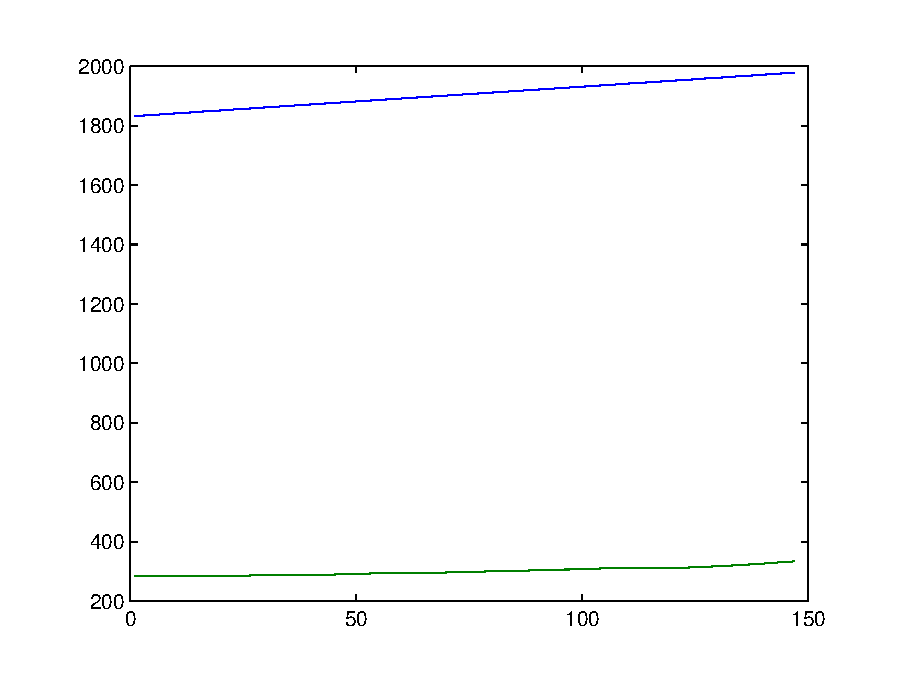
\includegraphics[width=\linewidth]{ch1-plot-icecore_default.eps}
\caption{Result of simply throwing the entire data matrix at \texttt{plot} ....}
\label{fig:ch1-plot-icecore_default}
\end{marginfigure}

You can do this step-by-step, and create yourself 2 vectors, one for the x-values and one for the y-values, and then \texttt{plot}:

\begin{docspec}
\textbf{>> X = etheridge\_etal\_1996(:,1);\\
>> Y = etheridge\_etal\_1996(:,2);\\
>> plot(X,Y);}
\end{docspec}

Or, if you are comfortable with more complex, single lines of code, go straight for the kill:

\begin{docspec}
\textbf{>> plot(etheridge\_etal\_1996(:,1),etheridge\_etal\_1996(:,2));}
\end{docspec}

Breaking things down into multiple bite-sized chunks rather than single long and complex lines,  is an equally valid way of doing things. It is longer ... taking 3 lines rather than 1, but the most important thing is to be happy that you understand what is going on. If breaking things down into multiple lines and creating new \textit{variables} helps -- \uline{DO IT}! Ultimately, and regardless of the method, you should end up with something like Figure \ref{fig:ch1-plot-icecore}.

\begin{marginfigure}[-2.0in]
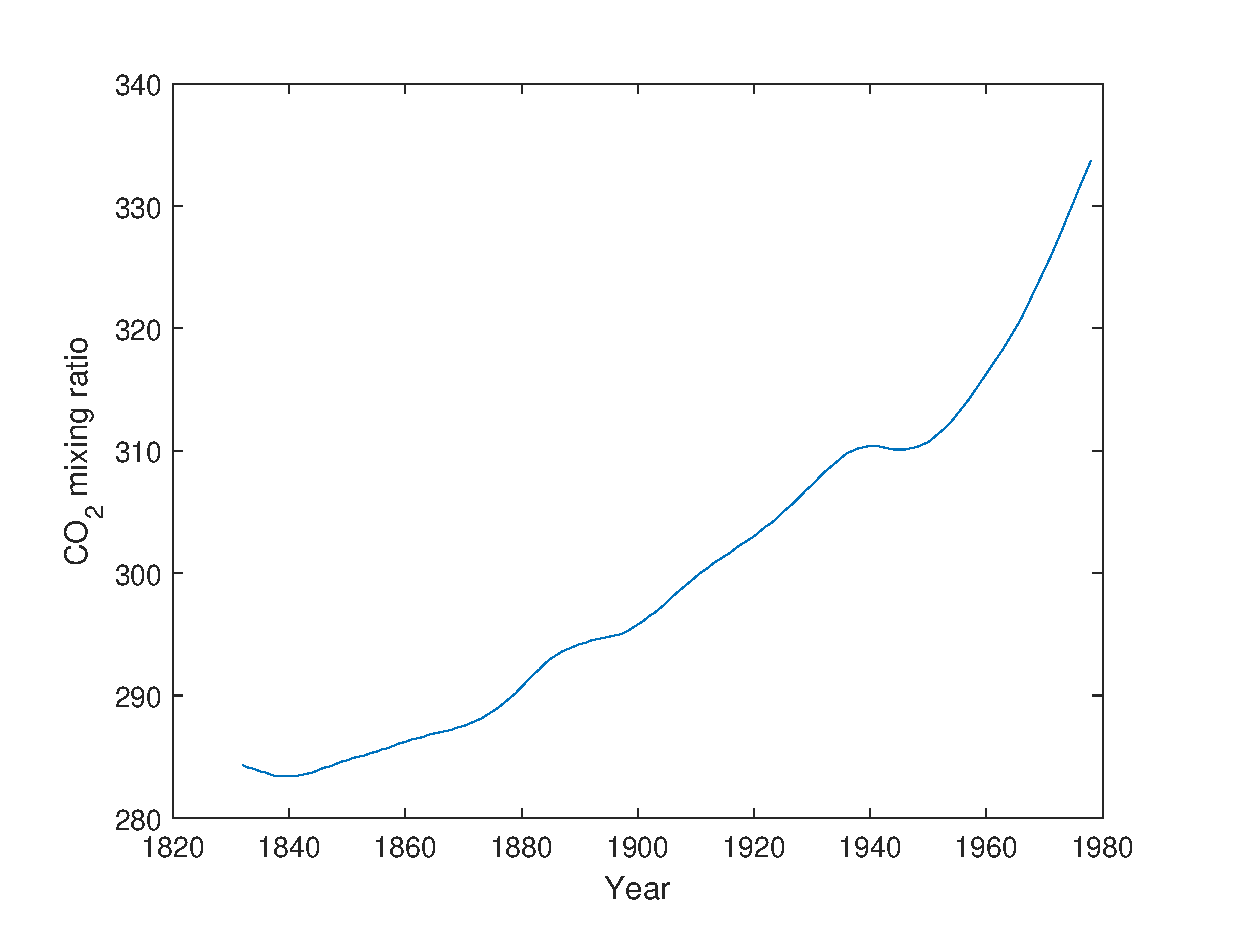
\includegraphics[width=\linewidth]{ch1-plot-icecore.eps}
\caption{Spline fit to measured changes in CO2 concentration in Law Done ice core, following \textit{Etheridge et al.} [1996].}
\label{fig:ch1-plot-icecore}
\end{marginfigure}

(If you plot ends up looking like Figure \ref{fig:ch1-plot-icecore_default} -- \uline{re-read the instructions carefully}.)

%------------------------------------------------

\subsection{Saving and exporting data}

Specific variables can  be saved in a plain text (ASCII format) by means of the \docenv{save} function (and then re-loaded in using \docenv{load}). You have to specify that you want a text format (rather than the default \textbf{MATLAB} \textsf{.mat} workspace format) -- see Box. Try re-saving the ice-core data as an ASCII format
text file (with a new filename) ... and then load it in again.

%------------------------------------------------

\subsection{Loading and saving the workspace}

The entire workspace (including all variables and their values, or just the values in a single variable if you wish) can be saved to a file and then later re-opened. The file format is specific to the \textbf{MATLAB} program and the file-name extension by default is \docenv{.mat}\sidenote[][-1.00in]{\textbf{MATLAB}'s proprietary file format for saving the contents of your current Workspace is indicated by a \docenvdef{.mat} file name extension (in Windoz).} You might find this very helpful to use in long lab exercise or large modelling projects, particularly if you do not come back to work at the exact same computer each time or wish to use continue the same piece of work on a laptop elsewhere. Try saving the current \textsf{Workspace}, then close down the \textbf{MATLAB} program. Re-running it, and then loading in your saved \texttt{.mat} file.
\sidenote[][-4.00in]{This sequence is going to look something like:
\begin{docspecmargin}
>> save MYSTUFF
\\>> exit
\end{docspecmargin}
...
\begin{docspecmargin}
load MYSTUFF
\end{docspecmargin}
Remember that when you re-start \textbf{MATLAB} you may have to change directories, add a path (\textsf{addpath}), or provide a full path to the \texttt{.mat} file, depending on where you saved it. 
}

\marginnote[-1.5in]{\begin{mdframed}[backgroundcolor=light-gray, roundcorner=10pt,leftmargin=1, rightmargin=1, innerleftmargin=5, innerrightmargin=5, innertopmargin=5,innerbottommargin=5, outerlinewidth=1, linecolor=light-gray]
\docenvdef{save}
\\Saves variables from the workspace to a file. There are two main forms (syntaxes) of the command:
\begin{docspecmargin}
>> save(FILENAME)
\end{docspecmargin}
which saves the entire workspace to a \textsf{.mat} file (with the filename given by the string \texttt{FILENAME} (in quotation marks), and:
\vspace{-4mm}
\begin{docspecmargin}
>>save(FILENAME,A,'-ascii')
\end{docspecmargin}
saves the data in the variable \texttt{A} (which must be given as a string, i.e. also enclosed in quotation marks) in plain text (ASCII) format. 
\\For example, if you had a variable \texttt{bananas}, and you want to save the contents (data) as the file \texttt{bananas\_data.txt}, you would write:
\vspace{-4mm}
\begin{docspecmargin}
>>save('bananas\_data.txt', ...'bananas','-ascii')
\end{docspecmargin}
(remembering this should be a single line and the \texttt{...} simply indicates that the line should be continuous)
\end{mdframed}}

Hopefully ... all your loaded/created variables etc. have been recovered ... ?

%------------------------------------------------

\newpage

%------------------------------------------------

\section{Basic data processing (and yet more plotting)}

This section runs through a couple of common basic data manipulation/processes techniques follow, plus some further plotting/visualization.

%------------------------------------------------

\subsection{Sorting data (in arrays)}

As an example to kick-off some data-processing tricks, load in the dataset of ('proxy') reconstructed atmospheric CO\(_{2}\) concentrations spanning the Phanerozoic: \textsf{paleo\_CO2\_data.txt} (labelled as 'Phanerozoic pCO2 proxy \uline{data}'). You can just import it into \textbf{MATLAB} using the \docenv{load} function as before -- remember the specific syntax of load:

\begin{docspec}
>> load(FILENAME)
\end{docspec}

\noindent where your \texttt{FILENAME} is \textsf{paleo\_CO2\_data.txt} and needs to be passed to load as a string, i.e.

\begin{docspec}
>> load('paleo\_CO2\_data.txt')
\end{docspec}

If you tell \textbf{MATLAB} nothing different (and do not assign the results of the \texttt{load} function to a different \textit{variable} name), \textbf{MATLAB} will again automatically create a \textit{variable} called \texttt{ paleo\_CO2\_data} (see \textsf{Workspace}) and assigned the loaded data into that.

If you view the contents of the variable\texttt{ paleo\_CO2\_data} (or whatever you might have passed the \texttt{load}-ed data to), you will see that there is a slight complication  -- unlike the ice core CO2 dataset, you now have 4 columns in this array\sidenote{Remember that you can diagnose its size with ... \texttt{size} (or refer to the Workspace window)}. The first column is age (Ma), the second the mean CO\(_{2}\) value, while the 3d and 4th columns are the low and high, respectively, uncertainty limits of the estimated past CO\(_{2}\) value.

Recalling how to reference specific columns of data in a matrix\sidenote{HINT: the \texttt{colon operator} (see earlier).}, and either referencing the columns of the array directly, or creating yourself separate vectors \texttt{X} and \texttt{Y} (see earlier) -- plot the mean paleo CO\(_{2}\) value as a function of age (in Ma). If you  closed the previous \textsf{Figure} window (see earlier), it is not essential to explicitly open one (using the \texttt{Figure} command) -- when you use the \texttt{plot} command, if there is no open \textsf{Figure} window, \textbf{MATLAB} will kindly open one for you. How thoughtful. The result of:

\begin{docspec}
>> plot(paleo\_CO2\_data(:,1),paleo\_CO2\_data(:,2));
\end{docspec}

\noindent (plotting the 2nd column out of the 4 columns, vs. the 1st column), should be something like \ref{fig:plot-CO2basic} ...

O dear ...

\begin{marginfigure}[-2.0in]
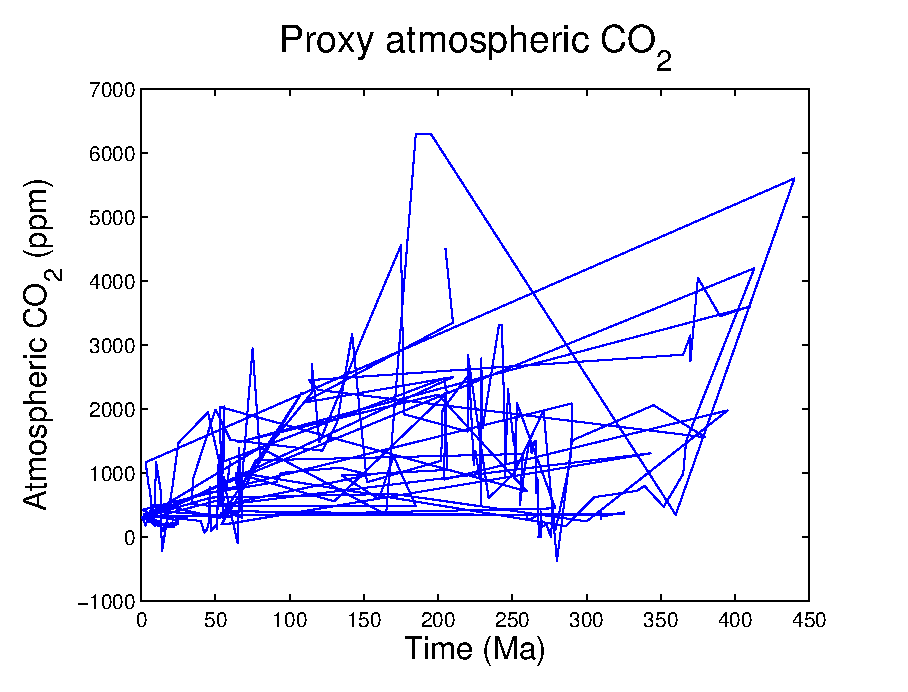
\includegraphics[width=\linewidth]{plot-CO2basic.eps}
\caption{proxy reconstructed past variability in atmospheric CO2.}
\label{fig:plot-CO2basic}
\end{marginfigure}

So ... that was not so successful. Why? What is happening in the default behaviour of \texttt{plot}, is that the (x,y) location defined by each subsequent row of data is being joined to the previous one with a line. This was fine for the ice-core CO2 example dataset because time progressed monotonically  in the first column, e.g. the data was ordered as a function of time. If you view the paleo CO\(_{2}\) data, this is not the case and time (age in Myr) does not progress monotonically in an always-getting-older (or always-getting younger) fashion.\footnote{In fact, in the original, full version of the data, ordering is by proxy type first, and then study citation, and only then age ...}

Your options are then:

\begin{enumerate}[noitemsep]
\setlength{\itemindent}{.2in}
\item You could import the data into \textbf{Excel}, then re-order (sort) it, then export (save) it, then re-load it ...
\vspace{1mm}
\item You could sort it in \textbf{MATLAB} using the \textit{GUI} variable view window. But lets not cheat for now.
\vspace{1mm}
\item You could sort it in \textbf{MATLAB} at the command line. How? Well, a reasonable gamble is to try:
\begin{docspec}
>> help sort
\end{docspec}
However, reading the \textsf{help} text \uline{carefully} (and you can always try it out and see what exactly it does if you are not sure), you will find that the \textit{function} \docenv{sort} will sort all columns \uline{independently} of each other, whereas we want the first column sorted and the remaining columns linked to this order. So this is not the \textit{function} that you are looking for.
\end{enumerate}

This is where it is worth paying attention to the bottom of \textbf{MATLAB} \textsf{help} and the \textsf{\uline{see also}} section. In this case, \textbf{MATLAB}\ lists \docenv{sortrows} as a possibility. The \textsf{help} text on this looks a little more promising. It is still slightly opaque (so also see Box), so the best thing to do is to try it (and view the results)! 

\begin{docspec}
>> sorted\_data = sortrows(paleo\_CO2\_data)
\end{docspec}

\noindent where the result of sorting the rows (of all columns) I have assigned to the variable \texttt{sorted\_data}. If you now try plotting this, e.g.

\begin{docspec}
>> plot(sorted\_data(:,1),sorted\_data(:,2));
\end{docspec}

\noindent it looks rather better -- Figure \ref{fig:plot-CO2basic2}. (This is a good illustration of a guess of a \textit{function} that was not quite what was needed, but following up on the \texttt{help} suggestions leads to a more appropriate \textit{function}.) At least now the curve is reminiscent of past changes in global temperature and the geological Wilson cycle, with high \(CO_{2}\) values in the Cretaceous and Jurassic and then lower again in the Carboniferous (roughly matching the progression of ice and hot house (and then back to recent ice ages) climates).

\marginnote[-6.0in]{\begin{mdframed}[backgroundcolor=light-gray, roundcorner=10pt,leftmargin=1, rightmargin=1, innerleftmargin=5, innerrightmargin=5, innertopmargin=5,innerbottommargin=5, outerlinewidth=1, linecolor=light-gray]
\docenvdef{sortrows}
\\In its simplest usage: 
\begin{docspecmargin}
>> B = sortrows(A)
\end{docspecmargin}
... "sorts the rows of a matrix in ascending order based on the elements in the first column. When the first column contains repeated elements, \texttt{sortrows} sorts according to the next column and repeats this behavior for succeeding equal values."
\\So, if the first column of the matrix was time, the data would be sorted into ascending time.
\\Beyond this usage, if you wanted to sort by a different column to the first, you would use:
\begin{docspecmargin}
>> B = sortrows(A,N)
\end{docspecmargin}
where \texttt{N} is the column number.
\\You can also sort in descending order:
\begin{docspecmargin}
>> B = ... sortrows(A,'descend')
\end{docspecmargin}
(ascend is the default).
\end{mdframed}}

\begin{marginfigure}[-1.5in]
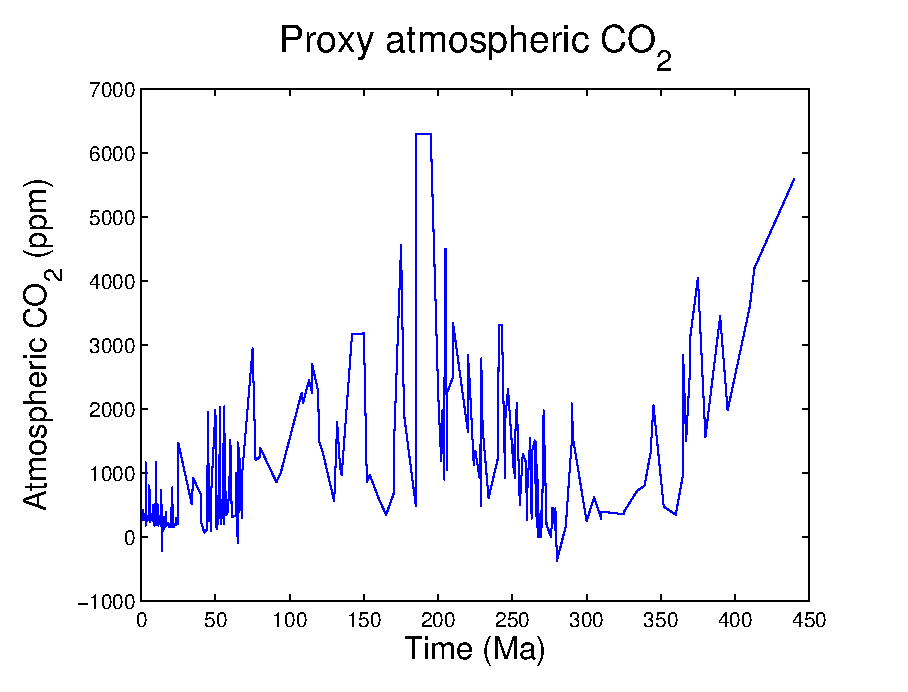
\includegraphics[width=\linewidth]{plot-CO2basic2.eps}
\caption{Proxy reconstructed past variability in atmospheric CO2 (sorted data).}
\label{fig:plot-CO2basic2}
\end{marginfigure}

A little later you will meet an alternative plotting \textit{function} that does not require the data to be sorted into any sort of order (\texttt{scatter}). But you should note that you can also use \docenv{plot}, but omitting the line segments by specifying only a symbol, e.g.

\begin{docspec}
plot(x,y,'ro');
\end{docspec}

\noindent (here, plotting circles for the data points in red) so that it does not matter in which order the individual points are plotted (and the same result is obtain from both sorted and un-sorted data).

%------------------------------------------------

\subsection{Data scaling}

\noindent As an example practicing some basic data scaling: download the historical global temperature anomaly dataset\sidenote[][-0.0in]{\href{https://www.ncdc.noaa.gov/cag/global/time-series/globe/land\_ocean/ytd/12/1880-2017/\#https://climate.nasa.gov/vital-signs/global-temperature/}{NOAA}}:

\vspace{1mm} \textsf{temperature\_globalanom.txt} \vspace{1mm}

\noindent (Labelled on the website as: 'Observed global mean temperature anomaly \uline{data}'.)

The columns are: (1) year, (2) annual mean ocean+land surface temperature \uline{anomaly} (i.e. temperature change relate to some reference value, where here is the observed 1901-2000 mean). Remember, you can \texttt{load} and assign data to an easier-to remember variable by e.g.:

\begin{docspec}
>> data1 = load('temperature\_globalanom.txt');
\end{docspec}

Plot the annual mean temperature anomaly for the full range of years, as per Figure \ref{fig:ch1-plot-temperature1}. (plus labels, title, etc etc), remembering again that you \uline{cannot} pass only the entire array to plot, as per:

\begin{docspec}
>> plot(data1);
\end{docspec}

\noindent but instead, must pass the 2 vectors (of x, and y-axis data), separately:

\begin{docspec}
>> plot(data1(:,1),data1(:,2));
\end{docspec}

\noindent (where e.g. \texttt{data1(:,1)} specifies all the rows of the 1st column of array \texttt{data1}).

\begin{marginfigure}[-4.5in]
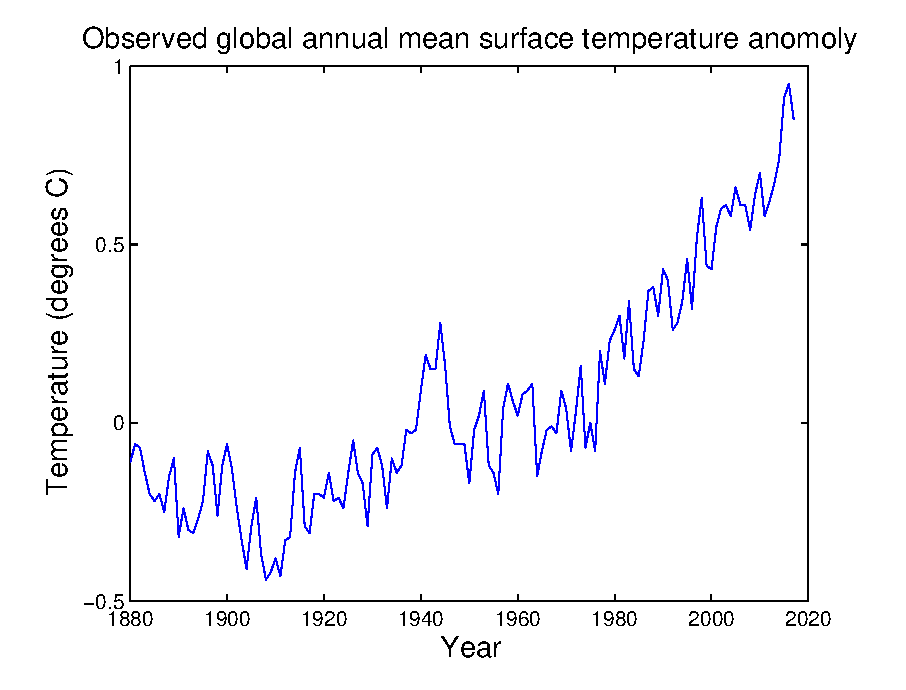
\includegraphics[width=\linewidth]{ch1-plot-temperature1.eps}
\caption{Observed annual global mean surface temperature anomaly (compared to year 1910 to 2000 average).}
\label{fig:ch1-plot-temperature1}
\end{marginfigure}

We are not going to transform the  data so that it is as an \uline{absolute}, rather than \uline{relative}, temperature. The 20th century average global temperature across land and ocean surface  is apparently 13.9\degree C. So first -- change the temperature anomaly data into absolute temperatures -- you'll do this by by adding the 20th century global average value, 13.9, to all the data values in the second column of your array.\sidenote[][-2.0in]{Remember -- you can increase the value of every element in an array, by simply adding that number, e.g. if \texttt{A} is you array of data, and \texttt{B} is a \textit{scalar} (the value you want to increase all array values by);
\begin{docspecmargin}
>> C = A + B;
\end{docspecmargin}
will have the effect of adding \texttt{B} to ever element in \texttt{A}, and assigning to a new array, \texttt{C}. Or alternatively, you can replace the contents of array \texttt{A} with the new values:
\begin{docspecmargin}
>> A = A + B;
\end{docspecmargin}
In your specific example:
\begin{docspecmargin}
>> data1(:,2) = ... 
\\data1(:,2) + 13.9
\end{docspecmargin}
(all one line) will have the effect of taking the 2nd column of the array \texttt{data1}, adding 13.9 to all the values, and writing the new values back into the 2nd column of the array \texttt{data1}.
} (If you are being good and reading the margin text ... the answer is there ...)

Now re-plot.

Next, convert the temperature units from \degree C to \degree F. An approximate conversion is:

\vspace{2mm}
\(T_{(\degree F)} = 1.8\times T_{(\degree C)} + 32 \)
\vspace{2mm}

\noindent where \(T_{(\degree F)}\) is the (new) temperature in \degree F, and \(T_{(\degree C)}\) the (old) temperature in \degree C.

For this, you will need to take your data (which is the 2nd column of the array), e.g. \texttt{data1(:,2)}, multilpy it by 1.8 as per the equation (\texttt{1.8*data1(:,2)}) and then add 32 (\texttt{1.8*data1(:,2) + 32})\footnote{If you have any doubts as to the order in which the operators are applied, add a set of parentheses, e.g. \\ \texttt{(1.8*data1(:,2)) + 32}}. And ... assign the results of this to a new vector or array. Or you can replace the original column (if you are feeling totally confident), e.g.

\begin{docspec}
>> data1(:,2) = 1.8*data1(:,2) + 32;
\end{docspec}
 
\noindent The aim is to obtain a modified data array in \textbf{MATLAB}, with year as the first column (year, as per the original data) but with the 2nd  column now being annual mean  temperature in units of \degree F.

If it helps -- play  the data conversion game in \textbf{Excel} first (e.g. creating new columns in a spreadsheet to firstly hold  absolute temperatures rather than anomalies, and then temperatures in \degree F rather than \degree C). Also if it helps -- create a new array with the modified temperature units data in (rather than replacing the 2nd column of  the original array, \texttt{data}). You can also do the conversion in 2 stages -- multiplying the (absolute) temperature (\degree C) by \(1.8\) first (perhaps creating a new array to hold this in), then adding \(32\).

Re-plot (in \textbf{MATLAB}) once again the final temperature trends in \degree F. This should look like Figure \ref{fig:ch1-plot-temperature3}.

\begin{marginfigure}[-2.0in]
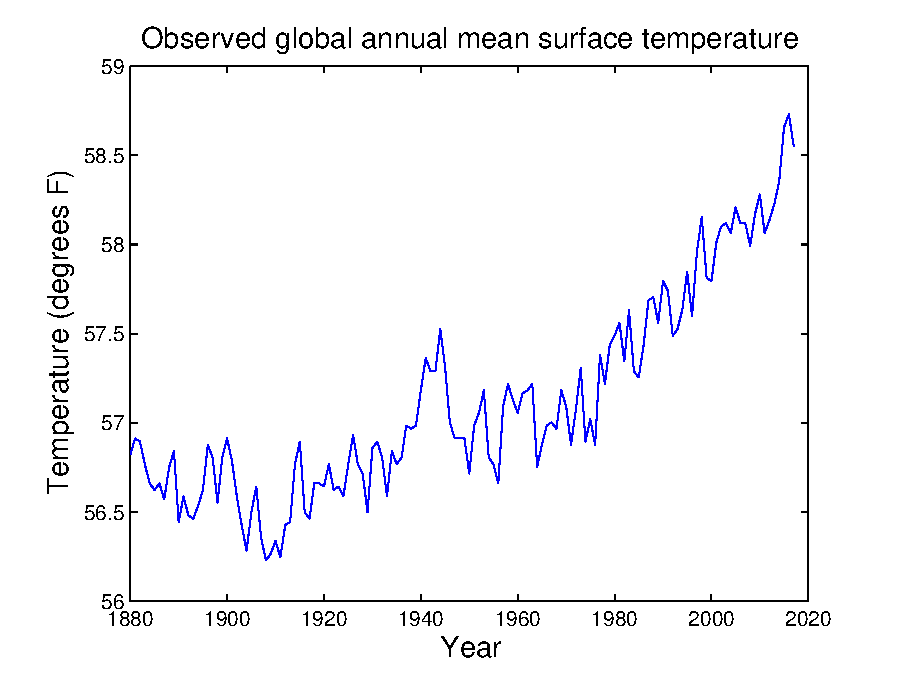
\includegraphics[width=\linewidth]{ch1-plot-temperature3.eps}
\caption{Observed annual global mean surface temperature.}
\label{fig:ch1-plot-temperature3}
\end{marginfigure}

%------------------------------------------------

\newpage

%------------------------------------------------

\section{Nicer graphing}

This section covers how to create slightly fancier plots in \textbf{MATLAB} and combines this with some more data loading practice.

%------------------------------------------------

\subsection{Modifying lines/symbols in \texttt{plot}}

The first deviant activity you can engage in with \texttt{plot}, is to graph the data without the line joining the points. Scrolling a little the way down \texttt{>> help plot}, it turns out that there are a number of options for color, line style, and marker symbol that you list together as a single parameter, straight after the parameters for \textit{x} and \textit{y} vectors. By default, \textbf{MATLAB} plots a solid line in blue with no marker points. Obviously, we could forego the sorting and plot a sane graphic (hopefully) by plotting just points and having no line between them. Hell, you could even be radical and use a different color ... Or, you could specify a symbol and no line.  The choice of colors is your oyster, as they (almost don't) say. e.g. Figure \ref{fig:plot-CO2basic3}. 

A summary of a few of the more common plotting options is provided in the Box. For any previous plot you have made, try changing the line style (or no line), and the marker shape and color.

\marginnote[-3.75in]{\begin{mdframed}[backgroundcolor=light-gray, roundcorner=10pt,leftmargin=1, rightmargin=1, innerleftmargin=5, innerrightmargin=5, innertopmargin=5,innerbottommargin=5, outerlinewidth=1, linecolor=light-gray]
The main (i.e. not an exhaustive list) data display options for the \texttt{plot} function are:
\\(1) point style
\\\noindent \texttt{.} -- point, \texttt{o} -- circle, \texttt{x} -- x-mark, \texttt{+} -- plus, \texttt{*} -- star, \texttt{s} -- square, \texttt{d} -- diamond, \texttt{v} -- triangle (down).
\\(2) line style
\\\noindent \texttt{-} -- solid, \texttt{:} -- dotted, \texttt{--} -- dashed, and when specifying a point style, not specifying a line style results in no line.
\\(3) color 
\\\noindent  \texttt{b} -- blue, \texttt{g} -- green, \texttt{r} -- red,  \texttt{y} -- yellow, \texttt{k} -- black, \texttt{w} -- white.
\\To use them, add a new parameter when you call the \docenv{plot} \textit{function} -- whereas before, you typed, for plotting a vector y against x:
\begin{docspecmargin}
plot(x,y);
\end{docspecmargin}
you now add, following a comma, the point and line style option you want, which must be encased in a pair of inverted commas, e.g. for a red, dashed line, you would type:
\begin{docspecmargin}
plot(x,y,'r--');
\end{docspecmargin}
and for blue circles (with no line):
\begin{docspecmargin}
plot(x,y,'bo');
\end{docspecmargin}
\end{mdframed}}

\begin{marginfigure}[-0.0in]
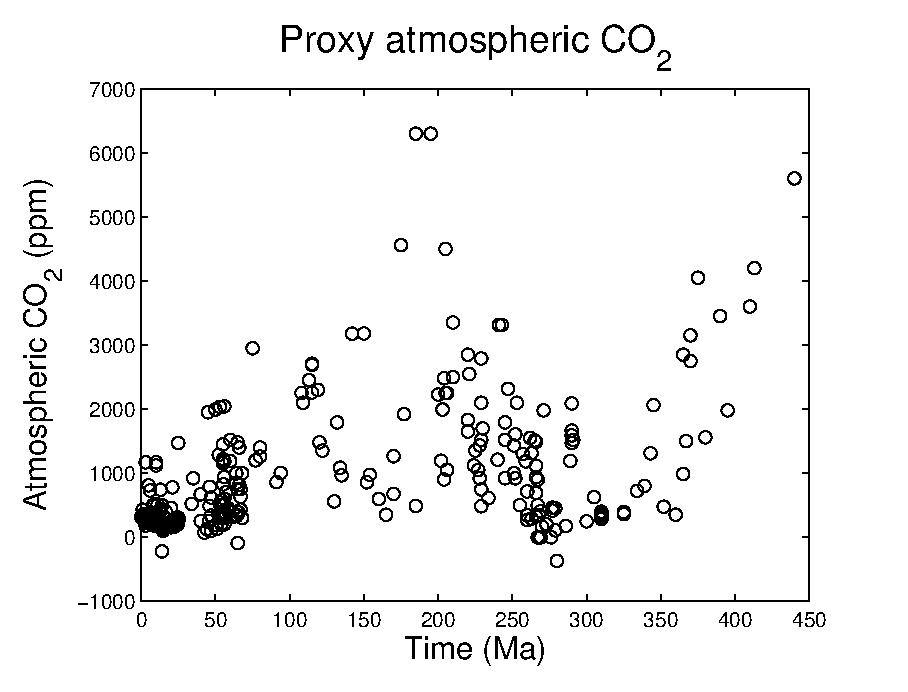
\includegraphics[width=\linewidth]{plot-CO2basic3.eps}
\caption{Proxy reconstructed past variability in atmospheric CO2 (sorted data).}
\label{fig:plot-CO2basic3}
\end{marginfigure}

%------------------------------------------------

\subsection{Plotting multiple data-sets}

So far, so good. But so boring, although simple marker-only and joined-by-line plots have their place. For a start, the original data-set included an estimate of the uncertainty in the \(CO_{2}\) reconstructions in the form of the min and max plausible value for each 'central' (best guess?) estimate. As a visual indication of the uncertainty in the \(CO_{2}\) reconstructions, one could plot the min and max values as points, using different symbols. This requires a further little trick in \textbf{MATLAB}, which involves the command \docenv{hold}. This is nice and simple and takes the additional (2nd) word: \texttt{on}, or \texttt{off}.
\\ \texttt{>> hold on} -- will enable you to add additional elements to a graphic,
\\ \texttt{>> hold off} -- returns to the default in which a new graphic replaces the current on in a Figure window. 

\vspace{1mm}
\noindent\rule{4cm}{0.5pt}
\vspace{-2mm}

\marginnote[-0.0in]{\begin{mdframed}[backgroundcolor=light-gray, roundcorner=10pt,leftmargin=1, rightmargin=1, innerleftmargin=5, innerrightmargin=5, innertopmargin=5,innerbottommargin=5, outerlinewidth=1, linecolor=light-gray]
\docenvdef{hold}
\\According to \textbf{MATLAB} \textsf{help}:
\\\texttt{hold on} -- retains plots in the current axes so that new plots added to the axes do not delete existing plots.
\\\texttt{hold off} sets the hold state to off so that new plots added to the axes clear existing plots and reset all axes properties.
\end{mdframed}}

\newthought{As an example} -- set:

\begin{docspec}
>> hold on
\end{docspec}

\noindent and then plot the minimum and maximum CO\(_{2}\) values (columns \#3 and \#4) in different symbols and different colors, on top of your existing plot. If you want to then label what the different lines or sets of points are, you can add a legend with the \docenvdef{legend} command. For instance, if you have managed to successfully plot the mean CO\(_{2}\) values as discrete black circles, and the minimum and maximum uncertainty limits as blue and red lines, respectively, you could type:
\begin{docspec}
>> legend('Mean CO\_2','Lower uncertainty limit','Upper uncertainty limit');
\end{docspec}
(all one line) and it should end up looking like Figure \ref{fig:plot-CO2basic4}.

\marginnote[-1.5in]{\begin{mdframed}[backgroundcolor=light-gray, roundcorner=10pt,leftmargin=1, rightmargin=1, innerleftmargin=5, innerrightmargin=5, innertopmargin=5,innerbottommargin=5, outerlinewidth=1, linecolor=light-gray]
\docenvdef{legend}
\\According to \textbf{MATLAB} \textsf{help}:
\\The command \texttt{legend} on its own, by default will label your datasets, 'data1', 'data2', etc etc, which is probably not what you want ...
\\So you have to supply strings -- one for each dataset plotted:
\vspace{-4mm}
\begin{docspecmargin}
legend('DATANAME1','DATANAME2', ...,'DATANAMEN');
\end{docspecmargin}
So if your plot had 2 greenhouse datasets -- 'CO2' and 'CH4', you would type:
\begin{docspecmargin}
legend('CO2','CH4');
\end{docspecmargin}
\end{mdframed}}

\begin{marginfigure}[-0.0in]
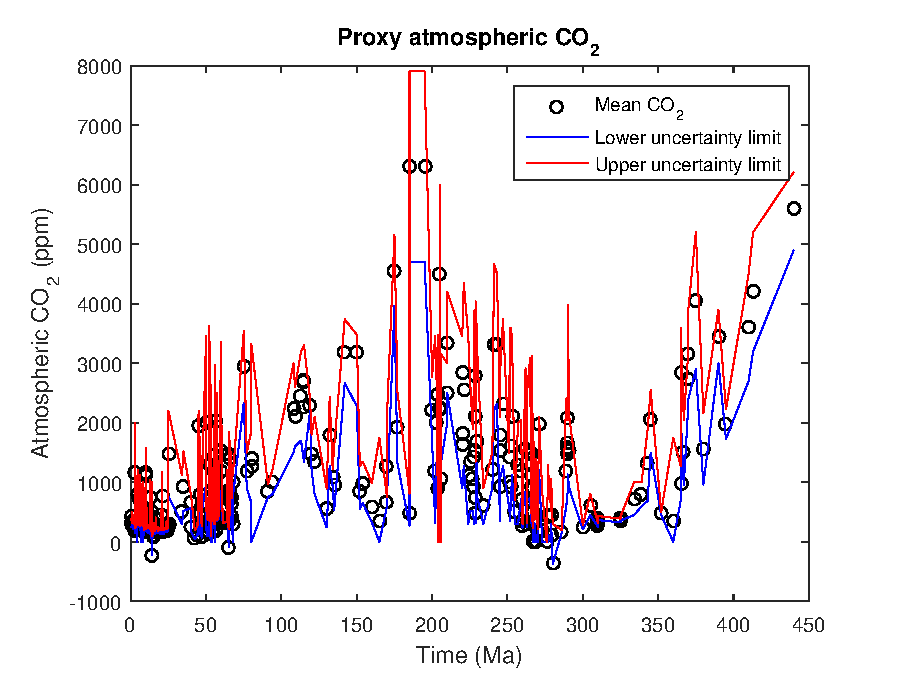
\includegraphics[width=\linewidth]{plot-CO2basic4.eps}
\caption{Proxy reconstructed past variability in atmospheric CO2 (sorted data).}
\label{fig:plot-CO2basic4}
\end{marginfigure}

\vspace{1mm}
\noindent\rule{4cm}{0.5pt}
\vspace{1mm}

\marginnote[-0.0in]{\begin{mdframed}[backgroundcolor=light-gray, roundcorner=10pt,leftmargin=1, rightmargin=1, innerleftmargin=5, innerrightmargin=5, innertopmargin=5,innerbottommargin=5, outerlinewidth=1, linecolor=light-gray]
\docenvdef{errorbar}
\\Works like \texttt{plot}, except it adds error bars. The 2 most useful usages are:
\\\texttt{errorbar(x,y,err)} plots y versus x and draws a vertical error bar at each data point. All of \texttt{x}, \texttt{y}, and \texttt{err}, are vectors (all of the same length).
\\\texttt{errorbar(x,y,neg,pos)}draws a vertical error bar at each data point, where neg determines the length below the data point and pos determines the length above the data point, respectively. All of \texttt{x}, \texttt{y}, \texttt{neg}, and \texttt{pos}, are vectors (all of the same length).
\end{mdframed}}

\noindent It is not something to worry about here (or even necessarily try), but just to make you aware that \textbf{MATLAB} has a function  -- 
\docenv{errorbar} -- to help you to visualize errors, including non-symmetric errors, relatively easily. (See \textbf{MATLAB} \textsf{help} and the margin Box.)

The complication here is that none of the options for \docenv{errorbar} allow for absolute values to be used for error plotting. So to use it in this particular example, we need to replace the absolute min, max column values, with their respective deviations from the mean value (2rd column). Hopefully, you can see the way to do this. For instance, to create an error for the maximum estimate (4th column):

\begin{docspec}
sorted\_data(:,4) = sorted\_data(:,4)-sorted\_data(:,2);
\end{docspec}

\noindent where we are saying: take all the values in the 4th column of the array, subtract the values in the 2nd column of the array, and assign the values back into the 4th column (hence replacing the absolute maximum estimate with the deviation of the maximum from the mean, i.e. the +ve error). (And then do similarly for the minimum values of the 3rd column.)

%------------------------------------------------

\subsection{Changing label font size (and type)}

The axis and title labels, by default, can be difficult to read when the graphics are saved and then imported into a document/paper. You can change the size of text as you create axis captions and figure titles etc., by specifying the value of an additional (text size) parameter in the function. For example, to increase the size of the x-axis label to a 14pt font:

\begin{docspec}
>> xlabel('Year','FontSize',14);
\end{docspec}

Here -- after the you have passed the string you wish to appear to the \textbf{MATLAB} \texttt{xlabel} \textit{function} (\texttt{'Year'}), there is a pair of additional parameters:

\begin{docspec}
'FontSize',14
\end{docspec}

The first additional parameter specifies the aspect of the axis label that you wish to change (here: \texttt{'FontSize'}), and the 2nd parameter of the pair, is the (new) value (here: \texttt{14}).\sidenote{See help on \texttt{xlabel}.} Similarly, the y-axis label and title text size can be adjusted in exactly the same way.

Other property parameters\sidenote{Again -- refer to \textbf{MATLAB} \textsf{help}.} that might be useful (to change), are (with example changes):

\begin{docspec}
'FontName','Courier'\\
'FontWeight','bold'\\
'FontAngle','italic'
\end{docspec}

\noindent (You can, of course, also adjust everyting about the look and feel of your plot via the figure window \textit{GUI}.)

%------------------------------------------------

\subsection{Scatter plots}

Returning back to the Phanerozoic proxy (CO\(_{2}\)) data, we can now put a different (graphical) spin on it.

\marginnote[-2.0in]{\begin{mdframed}[backgroundcolor=light-gray, roundcorner=10pt,leftmargin=1, rightmargin=1, innerleftmargin=5, innerrightmargin=5, innertopmargin=5,innerbottommargin=5, outerlinewidth=1, linecolor=light-gray]
\docenvdef{scatter}
\\"\textit{... creates a scatter plot with circles at the locations specified by the vectors x and y. This type of graph is also known as a bubble plot.}"
\\The simplest usage is:
\begin{docspecmargin}
scatter(X,Y)
\end{docspecmargin}
where is works pretty much like \texttt{plot}, except without the joining line segments. (\texttt{X} and \texttt{Y} are \textit{vectors} of the same length)
\begin{docspecmargin}
scatter(X,Y,20)
\end{docspecmargin}
specifies the marker size (in points), and:
\begin{docspecmargin}
\vspace{-4mm}
scatter(X,Y,20,'filled')
\end{docspecmargin}
then fills the markers. Finally:
\vspace{-3mm}
\begin{docspecmargin}
scatter(X,Y,20,Z,'filled')
\end{docspecmargin}
colors the points according to the data in the \textit{vector}, \texttt{Z}, or instead scales the marker size with \texttt{Z}, via:
\begin{docspecmargin}
\vspace{-3mm}
scatter(X,Y,Z,'filled')
\end{docspecmargin}
\end{mdframed}}

\begin{marginfigure}[0.0in]
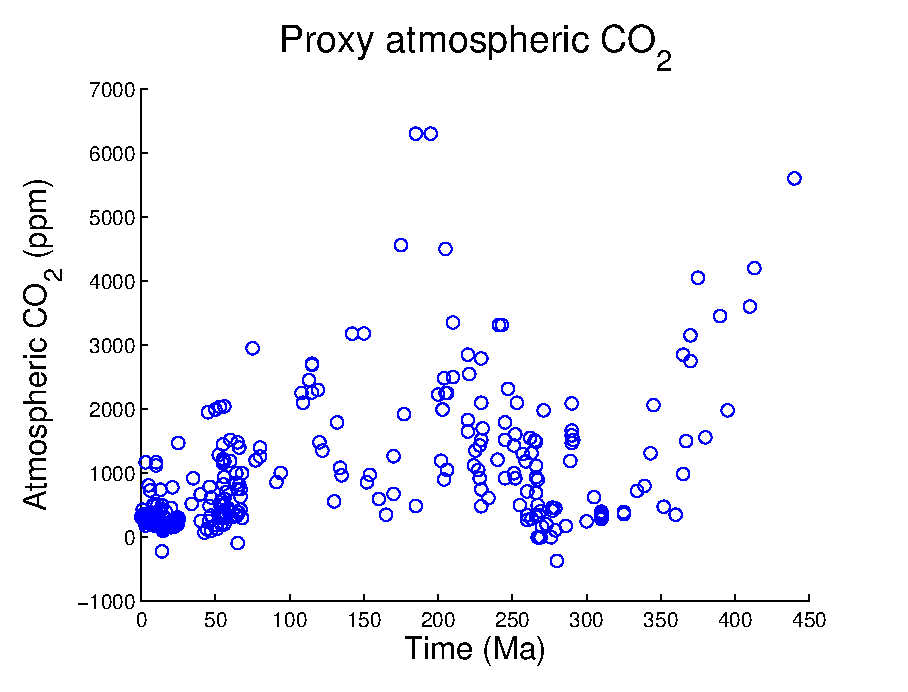
\includegraphics[width=\linewidth]{plot-CO2scatter.eps}
\caption{Proxy reconstructed past variability in atmospheric CO2 (scatter plot).}
\label{fig:plot-CO2scatter}
\end{marginfigure} 

Consider ... \docenvdef{scatter}. In fact, don't just considered it, \texttt{help} on it (\texttt{\textgreater\textgreater\ help scatter}). The simplest possible usage is, apparently:
\begin{docspec}
SCATTER(X,Y) draws the markers in the default size and color.
\end{docspec}
(where \texttt{X} and \texttt{Y} are vectors). This almost could not be more straight-forward.  Make yourself an \texttt{X} and \texttt{Y} vector out of the loaded-in dataset (or if you are feeling brave, you can pass in directly the appropriate parts of the dataset array), close the existing Figure window, and \texttt{scatter}-plot the (mean) CO\(_{2}\) data.

\begin{marginfigure}[-0.0in]
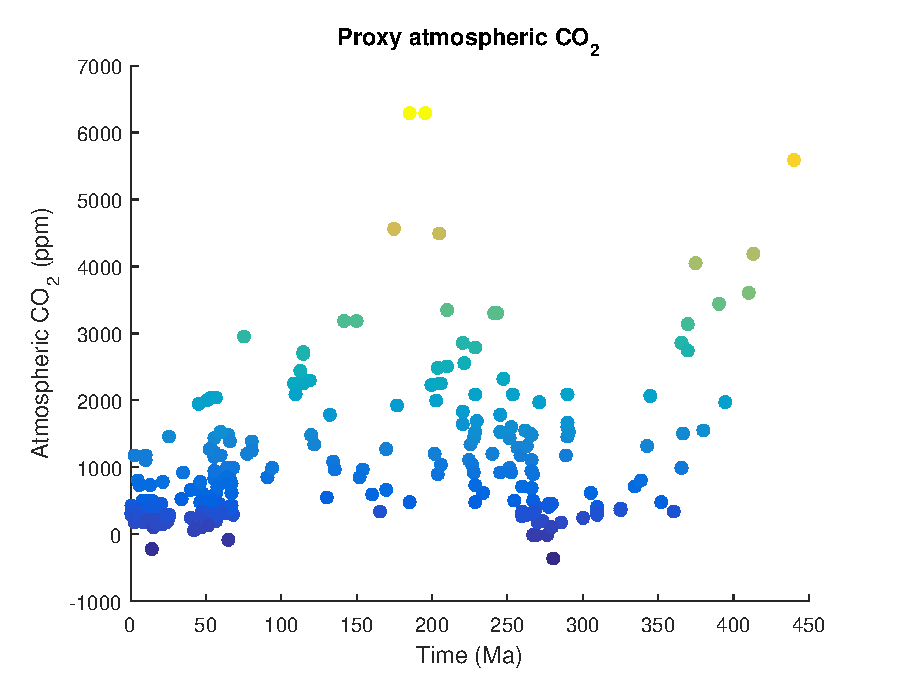
\includegraphics[width=\linewidth]{plot-CO2scatter2.eps}
\caption{Proxy reconstructed past variability in atmospheric CO2 (scatter plot).}
\label{fig:plot-CO2scatter2}
\end{marginfigure} 

Perhaps a little disappointingly, the default (Figure  \ref{fig:plot-CO2scatter}) (plus added labels) looks a little like one of the plots before. However, \texttt{scatter} can plot color-filled symbols, but more powerfully, can scale the fill color to a 3rd data value (vector), in a sort of pseudo 3D \textit{x}-\textit{y}-\textit{z} plot.  For instance, it will be duplicating information that is already presented (\textit{y}-axis), but you could color-code the points by the y-value, i.e. the atmospheric CO\(_{2}\) value. e.g.
\begin{docspec}
SCATTER(data(:,1),data(:,2),20,data(:,2))
\end{docspec}
draws the markers with an (area) size of 20 (points), in different colors. Coloring just the outlines of the circles is perhaps not ideal (difficult to see all of the color differences), so the circles can be filled in instead (and you could make them a little larger too):
\begin{docspec}
SCATTER(data(:,1),data(:,2),40,data(:,2),'filled')
\end{docspec}
resulting in Figure \ref{fig:plot-CO2scatter2}.

\vspace{1mm}
\noindent\rule{4cm}{0.5pt}

%------------------------------------------------

\subsection{Simple 2D data and bitmap visualization}

There are 2 different simple \textbf{MATLAB} commands for visualizing a 2D dataset (i.e. a matrix) as a bitmap image (and via a 3rd command, viewing various bitmap photo and image format files too).

As something (2D data) to play with -- \texttt{load} in the data matrix: \texttt{model\_grid.txt} (labelled as: '2D model grid \uline{data}'). Then, view the data in the array viewer, just to get a feel for what you are dealing with here (although you are unlikely to be much wiser after doing so). Lastly,  go ahead and employ the \docenv{pcolor} function in its simplest possible usage (see Box) to visualize the data. You can see (Figure \ref{fig:ch1-plot-pcolor1} ) that it is ... something. Maybe a little like the continents, but up-side-down at the very least. What to do?

Well, it is a good job that you remember how to re-orientate arrays, right? If you guess right first time (three different basic transformations of a matrix were described), you will get Figure \ref{fig:ch1-plot-pcolor2}.

\begin{marginfigure}[-3.5in]
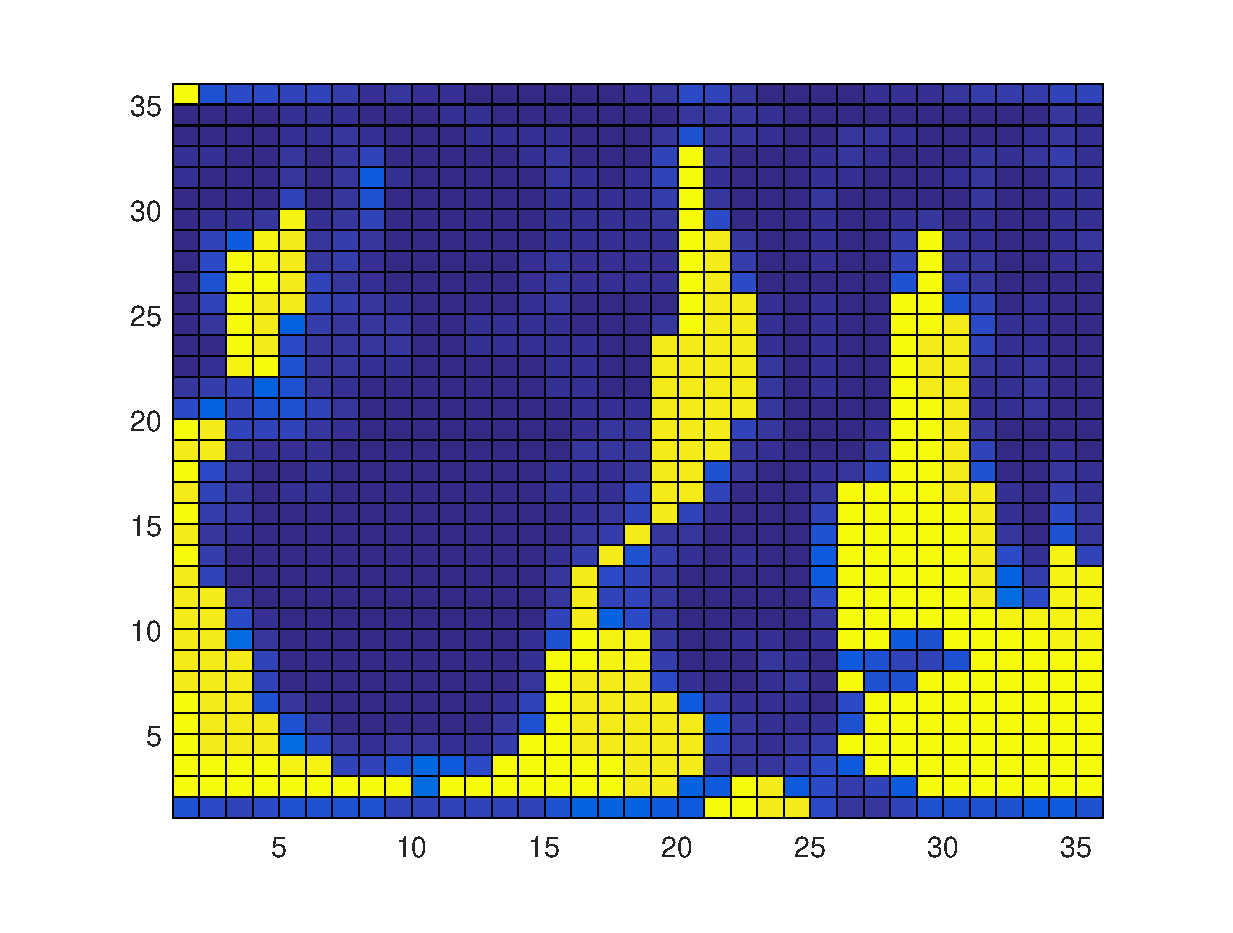
\includegraphics[width=\linewidth]{ch1-plot-pcolor1.eps}
\caption{A 2D plot of some random gridded model data.}
\label{fig:ch1-plot-pcolor1}
\end{marginfigure}

\begin{marginfigure}[-1.0in]
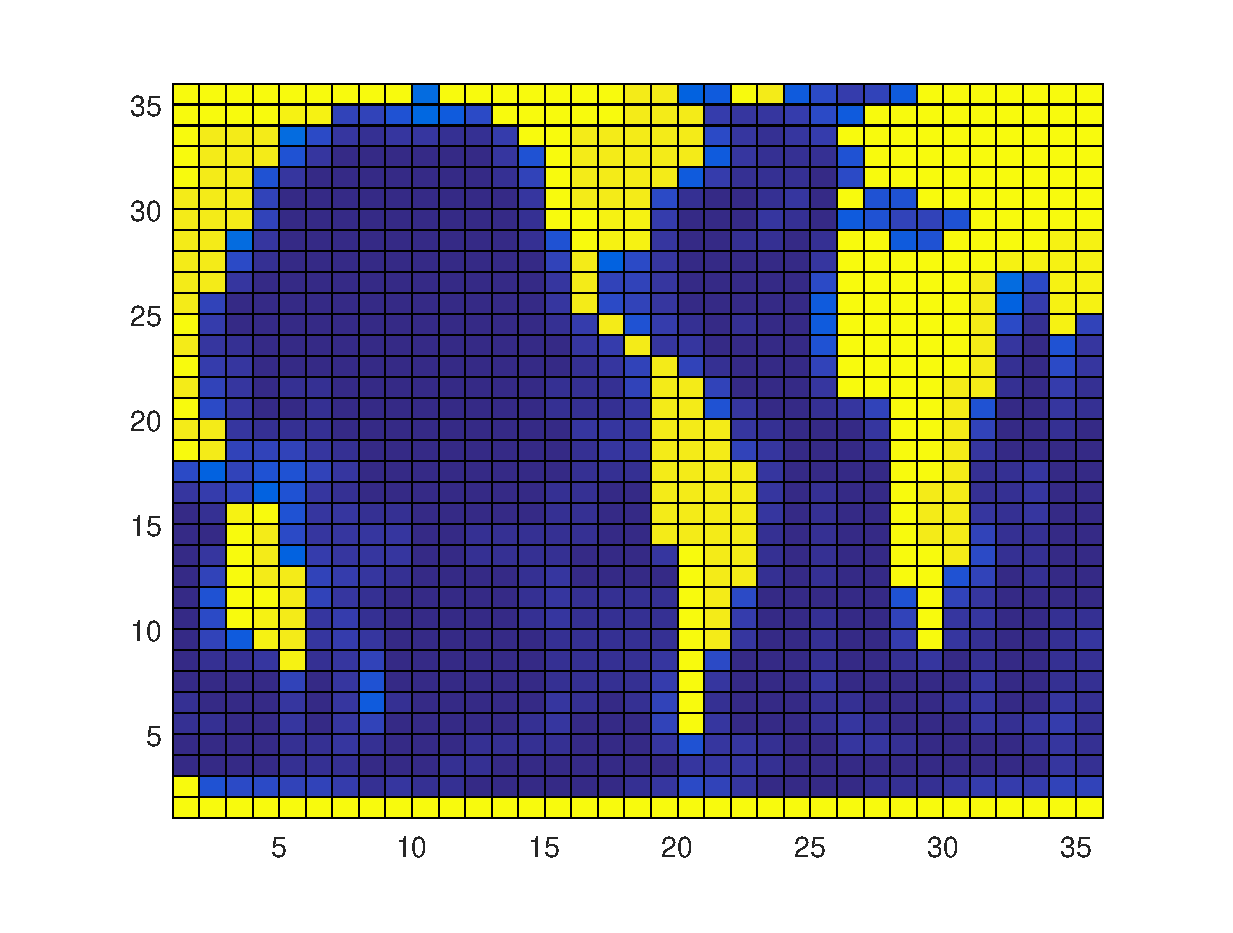
\includegraphics[width=\linewidth]{ch1-plot-pcolor2.eps}
\caption{A 2D plot of some random gridded model data ... but with the underlying data matrix re-orientated before plotting.}
\label{fig:ch1-plot-pcolor2}
\end{marginfigure}

Next try something very similar. but using the \docenv{image} function.\footnote{Now the model grid is the correct way around! I have absolutely no idea why and why it is reading the matrix dimensions differently from \docenv{pcolor}. I am sure you could \textbf{Google} and find out. But you would have to actually care first.} 

\marginnote[0.0in]{\begin{mdframed}[backgroundcolor=light-gray, roundcorner=10pt,leftmargin=1, rightmargin=1, innerleftmargin=5, innerrightmargin=5, innertopmargin=5,innerbottommargin=5, outerlinewidth=1, linecolor=light-gray]
\docenvdef{pcolor}
\\MATLAB claims that pcolor(C) plots; "a rectangular array of cells with colors determined by C. Actually, I believe \textbf{MATLAB} on this.
So if you have a matrix, \textbf{MATLAB} will plot a regular arrays of cells, with each cell representing one of the elements in the matrix, and will color that cell according to the value. (\texttt{pcolor} will by default, autoscale how the color scale maps onto the data in the matrix such that both extreme ends of the color scale are used.)
\end{mdframed}}

\marginnote[-0.25in]{\begin{mdframed}[backgroundcolor=light-gray, roundcorner=10pt,leftmargin=1, rightmargin=1, innerleftmargin=5, innerrightmargin=5, innertopmargin=5,innerbottommargin=5, outerlinewidth=1, linecolor=light-gray]
\docenvdef{image}
\\You can import an image, such as in \texttt{.jpg}, \texttt{.tiff}, or \texttt{.png} format, using \docenvdef{imread} -- simply pass it the name of an image file (as a string, this variable name needs to be encased in inverted commas) and assign the results to a variable name of your choice. Then plot (using \texttt{image}) that variable.
\end{mdframed}}

What is the point of this? You now have the ability to simply visualise a gridded dataset. Later, we'll be doing it more formally  and it gets rather more involved when you have to create matrixes to describe the grid dimensions (e.g. lon and lat) for yourself.

As your very last exercise -- find an image on the internet that amuses you, download it, load it into \textbf{MATLAB} (using \docenv{imread}), visualize it using \texttt{image}, and then ... well, that depends on how amusing it is. Maybe try plotting something on top of it (using \texttt{hold on}) or simply go home.

%------------------------------------------------

\newpage

%------------------------------------------------

\section{Further matrix math (systems of equations)}

%------------------------------------------------
%
You can also use \textbf{MATLAB}'s powerful matrix functionality to solve real-world problems for you.

\newthought{As an example} -- consider the Great Lakes -- the largest lake system in the world. They have on their shores some of the greatest cities ... as well as some of North Americas worst hockey teams. More importantly, much of the region is heavily industrialised and there is hence an exciting potential for pollution input into the lakes and hence a contrived numerical modelling exercise.

The layout of the lake system is shown schematically in Figure \ref{fig:ch4-lakes_schematic}, together with the mean volumes of the lakes and the annual flow rate of water out of them.

We can analyse the net result of a cocktail of heavy metals pouring into each lake, the amount dependent largely upon the population within the catchments of the lake. The assumed input rates to each of the 5 lakes are given below.

\begin{table}[h]\index{typefaces!sizes}
\footnotesize%
\begin{center}
\begin{tabular}{lccl}
\toprule
\ Lake & Heavy Metal Input (kg yr\(^{-1}\)) \\
\midrule
\ Superior & 1.0\(\times\)10\(^{3}\) \\
\ Michigan & 4.5\(\times\)10\(^{3}\) \\
\ Huron & 1.0\(\times\)10\(^{3}\) \\
\ Erie & 3.5\(\times\)10\(^{3}\) \\
\ Ontario & 3.0\(\times\)10\(^{3}\) \\
\bottomrule
\end{tabular}
\end{center}
\caption{Pollution input input rates to each of the 5 lakes.}
\label{tab:ch4-laketable}
\end{table}

The steady state concentration of heavy metals in the Great Lake system (the steady state solution being the state in which none of the concentrations in any of the lakes is changing) is something that you can find an analytical solution for. You have 5 unknowns (the concentration in each of the 5 lakes) and you can write down a series of 5 equations involving these unknowns. (There is slightly more to it than this, as there must also exist an inverse for the matrix, which is not always the case ...)

\begin{marginfigure}[0.0in]
\includegraphics[width=\linewidth]{ch4-lakes_schematic.tif}
\caption{Lake volumes and river flow rates in the Great Lakes system.}
\label{fig:ch4-lakes_schematic}
\end{marginfigure}

Lets call the concentrations (kg km\(^{-3}\)) of heavy metals in the lakes; \texttt{cS}, \texttt{cM}, \texttt{cH}, \texttt{cE}, and \texttt{cO} (for; Superior, Michigan, Huron, Erie, and Ontarion, respectively). At steady-state, the inputs of heavy metals must exactly balance the outputs from each lake (otherwise, the concentration in the lake would change and the system would not be at steady-state). We can write a series of mass-balance equations for the 5 lakes. For instance, in Lake Superior, the metal input flux is 1.0\(\times\)10\(^{3}\) kg yr\(^{-1}\) (1000 kg yr\(^{-1}\)). This must balance the loss of metals in the river outflow if the concentration of metals in the lake is to remain constant. The water outflow rate that is given to you is 63 km\(^{3}\) yr\(^{-1}\). The metal outflow flux is then just the concentration of metals in the water (\texttt{cS}), times by the water flow; \texttt{63*cS}. Thus, for Lake Superior, we can write \texttt{1000 = 63*cS}. The other lakes can be similarly analysed, to give a set of 5 equations:

\begin{docspec}
1000 = 63*cS 
\\4500 = 47*cM
\\1000 + 63*cS + 47*cM = 157*cH
\\3500 + 157*cH = 173*cE
\\3000 + 173*cE = 208*cO
\end{docspec}

It is not hard to work your way down these, solving first (\texttt{cS = 1000/63} is not so hard to solve ...) and then the 2nd, which then allows you to solve the 3rd, before then solving the 4th and 5th in turn .... However, the system of equations you might have to solve could be (and usually is) much more complicated. Fortunately, we can get \textbf{MATLAB} to do the work. :) It may be far from obvious what \textbf{MATLAB} has to do with this, so I'll do a little re-arranging of the 5 equations:

\begin{docspec}
\ 63*cS + \ \ 0*cM + \ \ 0*cH + \ \ 0*cE +  \ \ 0*cO = 1000
\\\ \ 0*cS + \ 47*cM + \ \  0*cH + \ \ 0*cE +  \ \ 0*cO = 4500
\\ -63*cS + -47*cM + 157*cH + \ \ 0*cE +  \ \ 0*cO = 1000 
\\\ \ 0*cS + \ \ 0*cM - 157*cH + 173*cE +  \ \ 0*cO = 3500
\\\ \ 0*cS + \ \ 0*cM + \ \ 0*cH - 173*cE + 208*cO = 3000 
\end{docspec}

This is starting to look scarily like some matrix stuff. Satisfy yourselves that these two sets of equations  are the same, and that all I have done is to write them with the unknowns on the left hand side (\texttt{cS}, \texttt{cM}, \texttt{cH}, \texttt{cE}, and \texttt{cO}) and the knowns (the metal input fluxes) on the right hand side. In fact, this can be written in matrix form:

\begin{docspec}
\(\begin{pmatrix}
63 & 0 & 0 & 0 & 0 \\
0 & 47 & 0 & 0 & 0 \\
-63 & -47 & 157 & 0 & 0 \\
0 & 0 & -157 & 173 & 0 \\
0 & 0 & 0 & -173 & 208 \\
\end{pmatrix}
\times
\begin{pmatrix}
cS \\
cM \\
cH \\
cE \\
cO \\
\end{pmatrix}
=
\begin{pmatrix}
1000 \\
4500 \\
1000 \\
3500 \\
3000 \\
\end{pmatrix}\)
\end{docspec}

Brush up on your matrix maths and check that this is exactly the same as before. It is just the series of 5 separate equations, but represented in matrix math form. Write out the matrix multiplication in full to get the 5 separate equations back again if you are not convinced that this is the case.

In a new \textbf{MATLAB} \textsf{m-file}, create a 5\(\times\)5 array containing the values in the matrix on the left hand side of the equation above and assign it to the variable \texttt{R} (for \uline{R}iver flow). Create a 5\(\times\)1 array containing the vector values on the right hand side of the equation and assign it to the variable \texttt{F} (for heavy metal \uline{F}lux). The solution to this problem is the set of (steady-state) concentrations of heavy metals in the 5 lakes. (Call this variable \texttt{C}.) We thus have the equation:
\begin{docspec}
\(R \times C = F\)
\end{docspec}

If we could determine the inverse of \texttt{R}, we could write:
\begin{docspec}
\(R^{-1} \times R \times C = R^{-1} \times F\)
\end{docspec}
\noindent (I have simply multiplied both sides of the equation by \texttt{R\(^{-1}\)}.)

Recognizing that a matrix (\texttt{R}) multiplied by its inverse (\texttt{R\(^{-1}\)}) is the Identity matrix (\texttt{I}), and that \texttt{I} leaves everything it multiplies alone, we have:
\begin{docspec}
\(I \times C = R^{-1} \times F\)
\\\(\Rightarrow C = R^{-1} \times F\)
\end{docspec}

We are there! We have \texttt{R} and \texttt{F}, so by multiplying \texttt{F} by the inverse of \texttt{R}, we get our set of 5 solutions (in the 5\(\times\)1 vector \texttt{C}). And \textbf{MATLAB} will give you the inverse of \texttt{R} (if it exists) on a plate.\sidenote{At the command line; type:
\begin{docspecmargin}
>> help inv
\end{docspecmargin}
to find out how to get your paws on the inverse of \texttt{R}. You can also lookup 'inverse of a matrix' in the Index of \textbf{MATLAB} Help.} Sweet deal!

Now you have everything you need -- go solve the steady-state problem for the unknown metal concentrations in the 5 lakes (the vector array \texttt{C}) using the inverse of \texttt{R}. You can always plug these values into the original equations  to satisfy yourselves that it all works out.\sidenote{Note that the equations above are written in normal maths language, e.g. with a \(\times\) rather than the \texttt{*} that \textbf{MATLAB} understands.}

%----------------------------------------------------------------------------------------
% CHAPTER 2
%----------------------------------------------------------------------------------------

\chapter{Elements of ... programming}
\label{ch:02}

%------------------------------------------------

\begin{fullwidth}

\newthought{Nerd.} This is what you are now going to become. And lose all your social skills. And sit at home all day in front of your computer. Which has become your only friend.

You will achieve this higher state of Being by starting to learn to write and use \textit{scripts} and \textit{functions} (aka \texttt{m-files}) in \textbf{MATLAB}. Actually, at this point you are now writing computer programs (of a sort) rather than endlessly typing stuff at the command line in the forlorn hope that something useful might occur.
You will also be doing a great deal of code debugging ...
\end{fullwidth}

%------------------------------------------------

\newpage

%------------------------------------------------

\section{Introduction to scripting (programming!) in MATLAB}

Commands in \textbf{MATLAB} can become very lengthy, and you typically end up with multiple lines of code to get anything even remotely useful done. And as you have noticed, it can take a lot of time to enter in all these lines. When when you log off and go home ... it is all gone. \sidenote[][-0.5in]{\textbf{MATLAB} remembers all the commands used in previous session (although this may not be the case of shared, lab computers) and lists them in the \textsf{Command History window}. You can recover and re-execute a previous command in this list by double-clicking it. You can also re-run more than one line at a time by selecting multiple lines and pressing \textsf{F9} (or \textsf{Evaluate Selection} from the (R-mouse button in \textbf{Windows}) context menu).} ... If only there was some way of storing all these commands in such a way that they could be worked on and run again with the press of a button (as a wild guess, how about \textsf{F5}?), without having to enter them all in, all over again from scratch ...

\marginnote{\begin{mdframed}[backgroundcolor=light-gray, roundcorner=10pt,leftmargin=1, rightmargin=1, innerleftmargin=5, innerrightmargin=5, innertopmargin=5,innerbottommargin=5, outerlinewidth=1, linecolor=light-gray]
\textit{\textbf{\textcolor[rgb]{0.501961,0,0}{m-file}}}
\\... is nothing more than a simple text file, in which a series of one or more \textbf{MATLAB} commands are written and which via the \textsf{.m} file extension, \textbf{MATLAB} interprets as a program file (\textit{script} or \textit{function}) that can be edited and executed (or rather, the list of commands inside, can be executed in sequential order).
\\Assume a similar convention to that for \textit{variables} in the naming of \textit{m-files}.
\end{mdframed}}

Your wish is granted! In \textbf{MATLAB}, it is possible to store all of your commands in a single text file, and then request that they (the list of commands) are all executed (sequentially)  at one go. \textbf{MATLAB} gives this text file a fancy name (because it is a very fancy piece of software, after all) -- a \textit{script}\sidenote{The conception of a \textit{function}, will be introduced later.}, otherwise known as an \textit{m-file}.  To create a new \textit{m-file}; from the  \textsf{File menu}, select \textsf{Script} (a common type of \textit{m-file})\sidenote[][0.0in]{In order version of \textbf{MATLAB}: \textsf{File}/\textsf{New} menu, and select: \textsf{Blank M-file}.}. You will see a text editor (more fancy-ness) appear in front of your very eyes, containing your requested (but currently empty) \textit{m-file}. Save the \textit{m-file} to your directory of choice. (Alternatively, simply create a new (blank) text file and save it with the extension \textsf{.m}, rather than e.g. \textsf{.txt} -- this creates you a (script) \textit{m-file}, illustrating that an \textit{m-file} is nothing more than a text file with a \textsf{.m} file extension.) From an \textit{m-file}, you can issue all the \textbf{MATLAB} commands you previously would have entered individually, line-by-tedious-line, at the command line. Furthermore, having created and saved  a \textbf{MATLAB} script, it can be executed again and as many times as you like.
 
You can execute an \textit{m-file} by typing its name into the \textsf{Command window} (\uline{omitting the \textsf{.m} file extension}). \uline{Ensure that \textbf{MATLAB} is operating in the same directory as the directory that you have saved your \textit{m-file}}. You can also run the \textit{script} (\textit{m-file}) by hitting the big bright green Run icon button at the top of the \textit{m-file} editor\sidenote[][-0.25in]{In older versions of \textbf{MATLAB} -- select: \textsf{Debug}/\textsf{Run} from the 'debug' menu of the \textsf{Editor window}.}. The short-cut for running it is to whack your paw down on the Function Key \textsf{F5}.

\marginnote[-1.0in]{\begin{mdframed}[backgroundcolor=light-gray, roundcorner=10pt,leftmargin=1, rightmargin=1, innerleftmargin=5, innerrightmargin=5, innertopmargin=5,innerbottommargin=5, outerlinewidth=1, linecolor=light-gray]
\docenvdef{disp}
\\... displays something (the contents of a variable) to the screen.
\\In the example of:
\begin{docspecmargin}
disp(STRING)
\end{docspecmargin}
where \texttt{STRING} is a .... \textit{string}, you get the \textit{string} displayed as text at the command line.
\\I n general, you can  pass the name of \uline{any} variable
\begin{docspecmargin}
disp(VARIABLE)
\end{docspecmargin}
and get the contents of \texttt{VARIABLE} displayed.
\\Note that the difference between using \docenv{disp} and simply typing the variable name:
\begin{docspecmargin}
>> VARIABLE
\end{docspecmargin}
is ... well, find out for yourself!
\\Note that there is no effect of including the semi-colon (\texttt{;}) at the end of \texttt{disp()}.
\end{mdframed}}

OK -- you are now ready for your very first program ... inevitably ... this has to be to print 'Hello, World' to the screen. No, really. (\textbf{Google} it.) 

Create a new \textit{m-file}, calling it e.g. \textsf{hello\_world.m} (remembering that spaces are NOT allowed in filenames). Make sure it is in the same directory  that \textbf{MATLAB} is working from ... You are going to use the function \docenv{disp} (see margin help box and/or type \texttt{>> help disp}  to find out the \textbf{MATLAB} \textit{function} syntax and usage). This command (/\textit{function})  will print to the screen, either any text you specify (in inverted commas), or the contents of any\textit{} \textit{variable} (you pass the variable name to \texttt{disp} (without inverted commas)). For now, simply pass the text directly.

Your program needs just a single line \uline{in the \textit{m-file}} (not at the command line):
\begin{docspec}
\textbf{disp('hello, world')}
\end{docspec}
\noindent Save the file (to your working directory). Run it at the command line by typing its name (omitting the \textsf{.m} extension):
\begin{docspec}
\textbf{>> hello\_world}
\end{docspec}

 Your first program is a success!(?)\sidenote[][-0.375in]{If \textbf{MATLAB} gives you an error message something like \\\textcolor{red}{\texttt{Undefined function or variable 'hello\_world'}} \\\noindent then it is likely you are simply not in the same directory as the \textit{m-file}, and/or the location of the \textit{m-file} is not in one of the directory paths \textbf{MATLAB} knows about (see previous Tutorials for comments on changing directory vs. adding paths.).} 

You could extend this to a mighty 2-line program by defining the string as a variable on the first line of the file (program), and displaying the contents of the variable (on the second). In a new \textit{script} \textit{m-file} (saved as e.g. \textsf{hello\_world2.m}), add the lines:
\begin{docspec}
message = 'hello, world ... again!';
\\disp(message)
\end{docspec}

\noindent and then save and run it.\sidenote[][0.25in]{Remember that when a \textit{function} requires a \textit{string} input, you can either pass the string directly (encased in inverted commas), or assigned the string to a variable, and pass the name of the variable (no inverted commas).}\sidenote[][0.0in]{If you get the message repeated twice, you might have committed the semicolon form the end of the first line.}

For further practice -- pick one of any of the previous exercises in which multiple lines of code were required, such as loading and then plotting a data set -- place these lines of code into a new \textit{m-file }(either by re-typing them in or copying them out of the \textsf{Command History window}), save the file (to the same directory that you are working from), and then run it my typing its name at the command line (omitting the \textsf{.m} extension).

%------------------------------------------------

\subsection{Programming good practice}

A few tips about good practice in (\textbf{MATLAB}) programming before we go on (and on and on and on):

\marginnote[-0.75in]{\begin{mdframed}[backgroundcolor=light-gray, roundcorner=10pt,leftmargin=1, rightmargin=1, innerleftmargin=5, innerrightmargin=5, innertopmargin=5,innerbottommargin=5, outerlinewidth=1, linecolor=light-gray]
\textbf{Creating \texttt{help} text in an \texttt{m-file}}
\\\textbf{MATLAB} allows you to crete a 'help' section in the \textbf{m-file} -- text that is outputted too the screen if you type help on that particular \textit{script} (or \textit{function}). The text is defined by a block of comment lines at the very top of the script file (or after the function definition in the case of a function). The last sequential comment line is taken to be the end of the help section. Note that the help section can be a minimum of eon single line.
A typical basic format is:
\begin{enumerate}[noitemsep]
\item Name of (in capitals), and very brief summary, of the script (/function).
\item List and description of the different forms of use (if there are one or more optional parameters) including definition of the input parameters.
\item Examples.
\item A \texttt{See also} section listing similar or related scripts or functions.
\end{enumerate}
\end{mdframed}}

\begin{itemize}[noitemsep]
\setlength{\itemindent}{.2in}

\item Choose helpful \textit{variable} names so that it is clear what each \textit{variable} represents. Avoid *excessively* short names, except for simple index and counting \textit{variables}. At the other extreme -- excessively long names, which the might be wonderfully descriptive, can lead to even simple calculation stretching over multiple lines of code (which can make it more difficult to see what is going on in the code overall). It is also very easy to create typos in trying to use very long \textit{variable} names.

\vspace{1mm}
\item Use comments within your \textit{m-file} to add explanation and commentary on your program. Anything after a \texttt{\%} on the same line is a considered a \textit{comment}\sidenote{Your \texttt{\% comment} can start on a new line, or follow on from the end of a line of code, whichever is more helpful.}, and is ignored by \textbf{MATLAB}.

\vspace{1mm}
\item Structure the code nicely. You can break the code up into sections, e.g. by adding a blank line. You might also start each section with a label (\textit{comment}) summarizing that it is going to do (via the addition of a \textit{comment} line).

\vspace{1mm}
\item To start with - create the- program in as simple a step-by-step way as possible. Breaking a complex calculation into several lines of simpler calculations is much easier to debug and work out what you were doing later, particularly if comments are also added. For all practical purposes -- at this level, everything will run just as fast whether as a complex calculation on one line, or simple bite-sized calculation spread over 4 lines with \textit{comments} in between. 

\vspace{1mm}
\item \uline{Always save your changes before running your program} (or you may unknowingly be running the previous version).

\vspace{1mm}
\item If using the \textit{script} to do some plotting, sometimes (but not always) it is convenient to add at the top of the \textit{m-file}, \begin{docspec}
close all;
\end{docspec}
This command close all currently open figures, plots, images, etc. so that if you repeatedly run the script such as you might in developing and debugging it, you don't end up with 1000000000s of \textsf{Figure windows} open ...

\end{itemize}

\vspace{1mm}
\noindent\rule{4cm}{0.5pt}
\vspace{2mm}\

\noindent An illustration (and a far from perfect illustration) of a short \textit{function} (\textit{m-file}) exhibiting at least a few examples of good practice, is:

\begin{marginfigure}[6.5in]
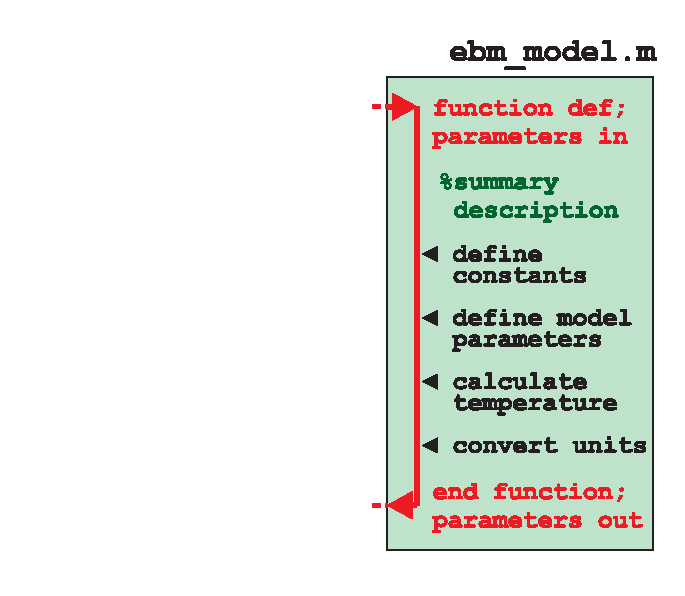
\includegraphics[width=\linewidth]{ch2-example.eps}
\caption{Schematic of the example program.}
\label{fig:ch2-example}
\end{marginfigure}

\begin{docspec}
\textcolor{blue}{function} [dum\_temp] = ebm\_basic(dum\_S0)
\textcolor[rgb]{0,0.501961,0}{\\\% 0D case of EBM -- analytical solution
\\\% function takes one parameter -- the solar constant (units of W m-2) [NB. modern value: 1370.0]
\\\% 
\\\% define constants}
\\const\_0C = 273.15; \textcolor[rgb]{0,0.501961,0}{\% (units: K)}
\\const\_sigma = 5.67E-8; \textcolor[rgb]{0,0.501961,0}{\% Stefan-Boltzmann constant (units: W m-2 K-1)}
\textcolor[rgb]{0,0.501961,0}{\\\% 
\\\% define model parameters}
\\par\_emiss = 0.62; \textcolor[rgb]{0,0.501961,0}{\% (non-dimensional)}
\\par\_albedo = 0.3; \textcolor[rgb]{0,0.501961,0}{\% mean albedo}
\textcolor[rgb]{0,0.501961,0}{\\\% 
\\\% solve for surface temperature
\\\% equilibrium equation:
\\\% (1.0-par\_albedo)*(par\_S0/4.0) = par\_emiss*const\_sigma*loc\_temp\(^{\wedge}\)4.0
\\\% then re-arranged to:}
\\loc\_temp = ( (1.0-par\_albedo)* ...
\\(dum\_S0/4.0)/par\_emiss/const\_sigma )\(^{\wedge}\)0.25;
\textcolor[rgb]{0,0.501961,0}{\\\% 
\\\% convert temperature units (Kelvin to Celsius) and set value of return variable}
\\dum\_temp = loc\_temp - const\_0C;
\textcolor{blue}{\\end}
\end{docspec} 

\noindent The schematic for the program structure is shown in \ref{fig:ch2-example}. (Don't worry what this particular program does, just note how I\ have structured it.)
 
This example also illustrates one possibility for a consistent \textit{variable} naming convention -- constants (\textit{variables} which never change in value) start with a \texttt{const\_} and parameters (variables whose values might be changed) with \texttt{par\_}, temporary ('local') variables with \texttt{loc\_} and variables passed into and out of the function: \texttt{dum\_}. Note the use of the semi-colon at the end of every line to prevent (here unwanted) printing of results to the screen. (Don't worry about what a \textit{function} is yet ... just not the degree of commenting and that there is some sort of consistent and meaningful naming convention.)

In the file, you can create as much 'ASCII art' as you like if it helps to make the code clearer, e.g. adding separator comment lines ...

\begin{docspec}
\textcolor[rgb]{0,0.501961,0}{\% ------------------------------------------------}
\end{docspec} 

... or highlighting certain section headers, e.g.

\begin{docspec}
\textcolor[rgb]{0,0.501961,0}{\% *** PLOTTING\ SECTION\ ***}
\end{docspec}

\noindent If it (a line) starts with a percentage symbol, then \textbf{MATLAB} ignores it and you can type whatever you like after it (on the same line).

\noindent Also note, if it helps -- you can run a single line of code over 2 lines of the file by adding:

\begin{docspec}
...
\end{docspec}

\noindent at the end of a partial line (that is to be treated by \textbf{MATLAB} as joined continuously to the next line).

\begin{marginfigure}[3.0in]
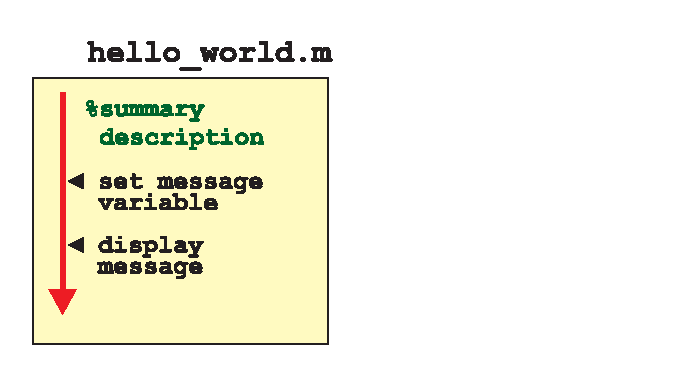
\includegraphics[width=\linewidth]{ch2-hello_world.eps}
\caption{Schematic of the Hello World program.}
\label{fig:ch2-hello_world}
\end{marginfigure}

Your \textsf{Hello World} program might look like the following once it has had a little tune-up (although in this example this is pretty much over-kill):
\begin{docspec}
\textcolor[rgb]{0,0.501961,0}{\\\% program to print 'Hello World' to the screen
\\\% *** START ***
\\\% first -- define the text to display and assign it 
\\\% \ \ \ \ \ \ \ \ to the variable  message}
\\message = 'hello, world';
\textcolor[rgb]{0,0.501961,0}{\\\% second -- display the contents of variable message}
\\disp(message)
\textcolor[rgb]{0,0.501961,0}{\\\% ***\ END ***}
\end{docspec}

The book schematic structure of this program (\textit{script}) is shown in Figure \ref{fig:ch2-hello_world}.\sidenote{Note that not all of the comment lines are shown in the structure schematic -- only the main program summary at the top.}

Finally, and related to the next subsection -- code in stages, testing the (partial) code at each step. \uline{Do not} try and write all the code in one go and only try it out at the end\sidenote{Because it will not work 99 times out of 100 ...}.

%------------------------------------------------

\subsection{Debugging the bugs in buggy code}

What programming is mostly about is not writing new code so much as debugging\sidenote{The art of fault-finding in computer code.} what you have already written. Key then, is to reduce the incidence of bugs occurring in the first place, and when they do occur, firstly to have code that lends itself to debugging and secondly, knowing how to go about the debugging. The first two facets are at least partly addressed through good programming practice (see earlier)\sidenote{And by the discipline of software engineering, which is way out of scope of this course.}.

Here is an example to try out to start to see what might be involved in debugging,  loosely based on a previous plotting example -- go create a new \textit{m-file} called: \textsf{plot\_some\_dull\_stuff.m}\sidenote{Remember -- you are advised to name your \textit{m-files} as something vaguely descriptive of what the script actually does (and you do ont have to go with this choice, although it might turn out to be perfectly descriptive ;) (i.e. you do not have to call it this!)}. Then add the following lines to the file (you can probably just directly copy-paste from the PDF file):

\begin{docspec}
\textcolor[rgb]{0,0.501961,0}{\% my dull plotting program
\\\% first, initialize variables and close existing \\\% figure windows}
\\close \textcolor[rgb]{0.501961,0,1}{all};
\textcolor[rgb]{0,0.501961,0}{\\\% set up variables to plot} 
\\x = -2*pi:0.1:2*pi;
\\y1 = sin(x); 
\\y2 = cos[x];
\textcolor[rgb]{0,0.501961,0}{\\\% open a figure window and plot the sine }
\\figure;
\\plot(x,y1,\textcolor[rgb]{0.501961,0,1}{'r'});
\textcolor[rgb]{0,0.501961,0}{\\\% add the cosine } 
\\hold \textcolor[rgb]{0.501961,0,1}{on};
\\plot(x,y2,k);
\end{docspec} 

\noindent and then \uline{save} and then run it (refer to earlier for how).

Pretty dull stuff eh? Wait -- maybe you didn't get a figure appearing on the screen with a pair of sines and cosines on. Has \textbf{MATLAB} given you an error? If you typed in the above 'correctly', you should see:
\begin{docspec}
\textcolor{red}{Error: File: plot\_some\_dull\_stuff.m Line: 6 Column: 9
Unbalanced or unexpected parenthesis or bracket.}
\end{docspec}

\noindent Actually ... if this were your program, you should have paid attention to earlier and not have written it all at once before testing it! But at least \textbf{MATLAB} is giving you some sort of feedback. The actual error reported might not always mean that much to you but the line number at which the problem occurred is gold-dust. The line of code is does not like is line 6\sidenote{Note that although \textbf{MATLAB} ignores comment lines (in the context of executing code), it does count them when telling you which line of the program code an error occurs at.}, which is:

\begin{docspec}
y2 = cos[x];
\end{docspec} 

\noindent Maybe the mistake is already obvious? If it is -- go fix it and re-run the program. If not, maybe test out the line more simply and in isolation (of the rest of the code) \uline{at the command line}, passing in a value directly to the function \texttt{cos} and not bother assigning the result to a different variable, e.g.

\begin{docspec}
>> cos[0.0]
\end{docspec} 

\noindent to which you get told:

\begin{docspec}
>> cos[0.0]
\textcolor{red}{\\ \ cos[0.0]
\\ \ \ \ \ \(\uparrow\)
\\Error: Unbalanced or unexpected parenthesis or bracket.}
\end{docspec} 

\noindent Now you have reduced the use of the \texttt{\texttt{cos}} command to its simplest, whilst retaining the usage in your program that seemed to cause an issue. Hopefully, now the error is apparent. If still not, check out help on the \texttt{cos} function, or search \texttt{cos} in the \textbf{MATLAB} help (from the question mark icon in the toolbar).

\textit{Is it important to recognise that (1) bugs will not always be flagged by \textbf{MATLAB} with a line number, and you can have valid code but nonsensical results, and (2) the mistake is often made earlier in the code than when \textbf{MATLAB} flags up a problem line.} 

\vspace{1mm}
Other strategies for helping debug include:

\begin{enumerate}[noitemsep]
\setlength{\itemindent}{.2in}
\vspace{0mm}
\item Checking  what the values of the variables were at the point at which the program derp-ed -- the current (and the point of program crash) variable values are listed in the \textsf{Workspace window}.
\vspace{1mm}
\item Changing the relevant variable value(s) (here \texttt{x}) and re-typing the problem line to see if it makes a difference\sidenote{This is sort of similar to the example given of simply testing a specific value directly.}.
\vspace{1mm}
\item Commenting out (\textcolor[rgb]{0,0.501961,0}{\%}) lines of code temporarily, or adding in additional (temporary) lines of code, and re-running. Where coding in bite-sized chunks is an advantage in this respect, is that if a program stops working after you have added a new section o code, you can go comment out the new code (never normally just delete it all), check that the original section of code still works, and then line-by-line, un-comment the new code until the problem line is found.
\vspace{1mm}
\item You can also put your program on hold just before the problem line and explore the state of the variables at that point (see Box), although in this particular example of a bug, \textbf{MATLAB} does not allow this, presumably because if feels that the mistake is simple and can be easily fixed. 
\end{enumerate}

\marginnote[-1.5in]{\begin{mdframed}[backgroundcolor=gray!10, roundcorner=10pt,leftmargin=1, rightmargin=1, innerleftmargin=5, innerrightmargin=5, innertopmargin=5,innerbottommargin=5, outerlinewidth=1, linecolor=light-gray]
\textbf{Debugging -- breakpoints}
\\\textit{Breakpoints} are indicators in the code that tell \textbf{MATLAB} to pause that that point. This allows for in-depth testing of variable values and lines of code without having to exit the program.
\\To add a \textit{breakpoint} in the code -- click in the (grey) margin of the code editor on the problem line or before, and \textbf{MATLAB} adds a red circle to indicate a 'breakpoint' has been set. The presence of a breakpoint tells MATLAB to pause that that line.
\\To unset a breakpoint, click on the red circle or you can clear one or more from the drop-down \textsf{Breakpoints} menu in the toolbar. 
\end{mdframed}}

Once you have fixed this, re-run the program. Ha ha -- it still does not work. (It is far from unusual to have multiple mistakes in the same piece of code, hence why writing the code in chunks and testing each time is helpful.)
\noindent Now we apparently have a problem on line 12:

\begin{docspec}
\textcolor{red}{Undefined function or variable 'k'.
\\ \
\\ Error in tmp2 (line 12)
\\ plot(x,y2,k);?}
\end{docspec}

\noindent Now \textbf{MATLAB} does not like \texttt{function or variable 'k'} because it cannot find that it has ever been defined. Is \texttt{k} meant to be a \textit{function} or \textit{variable}, or something else (e.g. a line style descriptor)? Look up \texttt{help plot} to remind yourself of the correct syntax if the problem is not immediately obvious.

Once you have fixed the second bug; saved, and re-run the script, you should see Figure \ref{fig:ch2-debug1}. (unless there were further bugs to find ...)

\begin{marginfigure}[-1.0in]
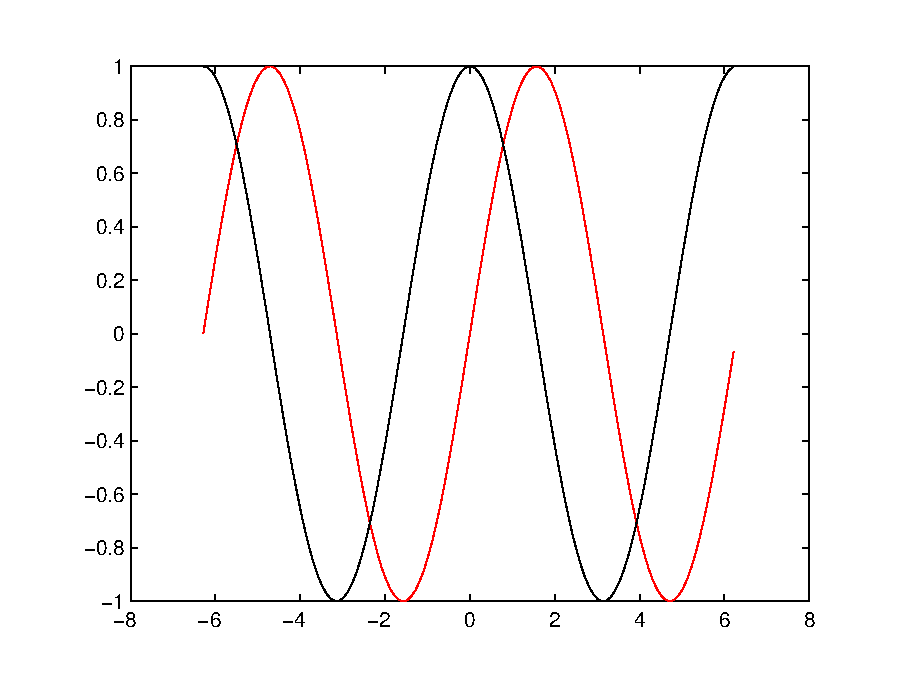
\includegraphics[width=\linewidth]{ch2-debug1.eps}
\caption{Output from the (bug-fixed version of) \textsf{plot\_some\_dull\_stuff} \textit{m-file}.}
\label{fig:ch2-debug1}
\end{marginfigure}

%------------------------------------------------

\newpage

%------------------------------------------------

\section{Functions}

\textit{Functions} in \textbf{MATLAB}, are really just fancy \textit{scripts}. Again -- just plain old lines of code in a text file that is given a \textsf{.m} extension (making it an \textit{m-file}). The big difference from a \textit{script} in \textbf{MATLAB} is that a \textit{function} can take variables as input and/or return variables (or variable values) as an output. (In contrast, a \textit{script} takes no input and returns no outputs, other than plots or data files that might be saved.) 

A \textit{function} is defined (and differentiated from a \textit{script}) by a special line at the \uline{very start}\sidenote{Literally: line 1. Not even a comment line is allowed to appear before the \textit{function} definition line.} of the \textit{m-file} (see Box). \uline{You must follow the \textbf{MATLAB} syntax exactly in defining a function.}

\marginnote{\begin{mdframed}[backgroundcolor=gray!10, roundcorner=10pt,leftmargin=1, rightmargin=1, innerleftmargin=5, innerrightmargin=5, innertopmargin=5,innerbottommargin=5, outerlinewidth=1, linecolor=light-gray]
\textit{\textbf{Functions}}
\\The all-important fancy first line of a \textit{function}, as defined in \textbf{MATLAB} help, looks like:
\begin{docspecmargin}
function [y1,...,yN] = myfun(x1,...,xM)
\end{docspecmargin}
Thanks \textbf{MATLAB} (this seems overly complex to say the least)!
\\OK -- lets break this down. Lets assume that you call the \textbf{m-file} calc\_stuff. The minimal definition of a function then looks like:
\begin{docspecmargin}
function [] = calc\_stuff()
\end{docspecmargin}
(The \textit{syntax} is critical and the definition line must look like this.) Here we are saying -- pass in not parameters and return no values either. So exactly like a normal script would work and you would execute the function calc\_stuff by typing at the command line:
\begin{docspecmargin}
>> calc\_stuff()
\end{docspecmargin}
(Maybe you can get away without the \texttt{()} bit.)
\\If you wan to pass in a single parameter (here: X), then you define the function:  
\begin{docspecmargin}
function [] = calc\_stuff(X)
\end{docspecmargin}
(To pass in more than 1 variable, simply comma separated the variable names.)
\\To pass out a parameter (here: Y) (and no input):
\begin{docspecmargin}
function [Y] = calc\_stuff()
\end{docspecmargin}
Lastly, at the end of the function, you include the line:
\begin{docspecmargin}
end
\end{docspecmargin}
\end{mdframed}}

This is all not as weird as you might think. For example, you have already used the \textit{function} \texttt{sin} -- this takes a single input (angle in radians), and returns a single output (the sine of the angle). If you were to write your own function for \texttt{sin}, the file would start something like:
\begin{docspec}
function [Y] = sin(X)
\end{docspec}
You can't, of course, go re-defining pre-defined \textbf{MATLAB} function names\sidenote{Actually you can, but it is best not to.}. So how about if in your work, you found you frequently needed to use the square of the sine of a number. You could keep writing:
\begin{docspec}
Y = (sin(X))\(^{\wedge}\)2
\end{docspec}
\noindent or, if you were a little more devious, you could create your own \textit{function} for returning the square of the sine of a number. 

In this example, the contents of your \textit{m-file}, which here we'll call \textsf{sin2}\sidenote{And hence filename \textsf{sin2.m}.}, would look like:
\begin{docspec}
\textbf{function [Y] = sin2(X)
\\Y = (sin(X))\(^{\wedge}\)2; 
\\end}
\end{docspec}
\noindent but of course with \uline{lots} of comments to remind you what the \textit{function} does etc. (Try this out -- create a new blank \textit{script} \textit{m-file}, add this code, save the file, and run it.)

Your new \textit{function} is used pretty much as you would expect and have used previously, e.g.
\begin{docspec}
>> sin2(0.5)
\end{docspec}
\noindent will return the square of the sine of a value of 0.5 and dump the answer to the command line, and 
\begin{docspec}
>> Y = sin2(0.5);
\end{docspec}
\noindent does the same but assigns the answer to the variable \texttt{Y} (with the semi-colon suppressing output to the command line).

NOTE that you can make a new function in 2 different ways:
\begin{enumerate}[noitemsep]
\vspace{1mm}
\item Create a new (blank) \textit{script} \textit{m-file}.
\\By adding the function definition line on the very first line of the file (e.g. \texttt{function [] = calc\_stuff()}), and \texttt{end} at the end, you turn the \textit{script} into a \textit{function}.
\vspace{1mm}
\item From the \textbf{MATLAB} \textsf{Editor} or main window menu, you can also chose: \textsf{New} -> \textsf{Function}.
\\This creates you a generic \textit{function} template file with a bunch of lines of stuff already in it:
\begin{docspec}
\textcolor{blue}{function} [outputArg1,outputArg2] = untitled3(inputArg1,inputArg2)
\\\textcolor[rgb]{0,0.501961,0}{\%UNTITLED3 Summary of this function goes here
\\\%   Detailed explanation goes here}
\\outputArg1 = inputArg1;
\\outputArg2 = inputArg2;
\\\textcolor{blue}{end}
\end{docspec}
If you find this too confusing, particularly early on in the course, just stick to method (1).
\end{enumerate}

NOTE2: You \uline{do not} want \textbf{MATLAB} \textbf{Live Script}.

\vspace{1mm}
\noindent\rule{4cm}{0.5pt}
\vspace{2mm}

\noindent Now go practice and make up your own \textit{function}. Start by creating one that takes a single input and returns a value equal to the sine of the square of the value (rather than the square of the sine as above). Test it (i.e. compare the output of your \textit{function} with the equivalent calculation typed in at the command line).

When you are happy with this, create one with 2 inputs (refer to \textbf{MATLAB} \texttt{help} on \texttt{function} and/or refer to the previous Box), that returns a value equal to the sine of the first input, divided by the cosine of the second input\sidenote{Mathematically, the answer is not valid for all possible values of the 2 inputs (why?), and later we'll learn how to pro-actively deal with such a situation.}, i.e.

\vspace{2mm}
\(y = \frac{sin(x_1)}{cos(x_2)}\))
\vspace{2mm}

Note that you have used other \textit{functions}, perhaps without knowing it, and some of them return values, but because you have not attempted to assign the returned values to a variable, you may not have not noticed. For example, \texttt{plot} and \texttt{scatter} are in fact \textit{functions}, and return an ID of the plot graphic. We simply have not been asking for the returned value so far. As per \textbf{MATLAB} \texttt{help}:
\begin{docspec}
H = SCATTER(...) returns handles to the scatter objects created.
\end{docspec}
with the \texttt{handle}, \texttt{H}, being an identifier of the graphic which could prove to be useful if  e.g. you would like to modify  one of the properties of an existing graphic.

\marginnote[-1.5in]{\begin{mdframed}[backgroundcolor=gray!10, roundcorner=10pt,leftmargin=1, rightmargin=1, innerleftmargin=5, innerrightmargin=5, innertopmargin=5,innerbottommargin=5, outerlinewidth=1, linecolor=light-gray]
\textbf{Debugging -- \textit{functions}}
\\\textit{Functions} are a prime example of the importance of being able to pause code part the way through (e.g. by setting a \textit{breakpoint}) because when a \textit{function} terminates, or crashes, you get to see none of the values of any variables created within the \textit{function}, unless they have been returned as output (and assuming here that the code did not crash and managed to get to the end). Setting a \textit{breakpoint} allows you to interrogate the values of any internal \textit{variables}.
\end{mdframed}}

Finally, it is important to note that by default, any variables created within a \textit{function} are TOP SECRET, and by that, I mean that they are not accessible to the main \textbf{MATLAB} workspace and do not appear listed in the \textsf{Workspace window}. To see that this is a non-Trumpian \uline{true fact}, create the following \textit{function} (basically, the first example but split into 2 steps):
\begin{docspec}
\textcolor{blue}{function} [Y] = sin2new(X)
\\tmp = sin(X);
\\Y = tmp\(^{\wedge}\)2; 
\\\textcolor{blue}{end}
\end{docspec}
\noindent Here, we have created a variable \texttt{tmp} to hold the value of the partial calculation. It does not appear in the \textsf{Workspace window} when you use the \textit{function}. The advantage of this is that you could create a second \textit{function} that also created a temporary variable internally called \texttt{tmp} with both instances of \texttt{tmp} treated entirely sperate and isolated by \textbf{MATLAB} (i.e. setting the value of one instance of \texttt{tmp} does not affect the value of the other).

The private nature of \textit{variables} created within \textit{functions} does however does lead to some additional complications in debugging \textit{functions} because when the function terminates, you have no record of what occurred during its execution (in terms of not being able to access the value of any of the variables used within the \textit{function}). Try setting a breakpoint at the start of the line where the square of \texttt{tmp} is calculated -- note that \texttt{tmp} now appears in the \textsf{Workspace window}. Continue the \textit{function} and when it terminates, note that \texttt{tmp} is now gone from the list.

%------------------------------------------------

\newpage

%------------------------------------------------

\section{Conditionals '101'}

%------------------------------------------------

\subsection{\texttt{if ...}}

One of the most important programming constructs is the \textit{conditional statement}, in which whether one or more \textit{statement}(s) are executed (and hence the overall outcome) is \uline{conditional} on the 'truth' or otherwise (i.e. it being true or false) of a given \textit{expression}.\sidenote{Pause ... and deep breath.}

\marginnote[-0.0in]{\begin{mdframed}[backgroundcolor=gray!10, roundcorner=10pt,leftmargin=1, rightmargin=1, innerleftmargin=5, innerrightmargin=5, innertopmargin=5,innerbottommargin=5, outerlinewidth=1, linecolor=gray!10]

\textbf{Conditional Statements}
\\The principal \textit{conditional statement} in \textbf{MATLAB} is: \docenvdef{if ... end}
\\The basic \texttt{if} structure is:
\begin{docspecmargin}
if EXPRESSION (IS TRUE)
\\ \ \ \ STATEMENT(S)
\\end
\end{docspecmargin}
in which the code \texttt{CODE} is executed if \texttt{EXPRESSION} is evaluated as \texttt{true}. No code is executed otherwise (and \texttt{STATEMENT} is \texttt{false}).

A variant addition -- \docenvdef{else} -- which allows for an alternative block of code (\texttt{OTHER STATEMENT(S)}) to be executed if \texttt{EXPRESSION} is instead evaluated as \texttt{false}, is:
\begin{docspecmargin}
if EXPRESSION (IS TRUE)
\\ \ \ \ STATEMENT(S)
\\else
\\ \ \ \ OTHER STATEMENT(S)
\\end
\end{docspecmargin}
Finally, there is 3rd variant including \docenvdef{elseif}:
\begin{docspecmargin}
if EXPRESSION (IS TRUE)
\\ \ \ \ STATEMENT(S)
\\elseif EXPRESSION (IS TRUE)
\\ \ \ \ OTHER STATEMENT(S)
\\else
\\ \ \ \ OTHER STATEMENT(S)
\\end
\end{docspecmargin}
Now, assuming that the first \textbf{EXPRESSION} is not true, a second \textbf{EXPRESSION} is evaluated, and only if that second \textbf{EXPRESSION} is also not true, will the final possible \textbf{STATEMENT} be evaluated. (Here, this final variant is shown with an \texttt{else ...} included at the end, but this is not a formal requirement to include.)

\end{mdframed}}

This is embodied in \textbf{MATLAB} (and similarly in most languages) by the \docenv{if ... end} construct (see \textit{Conditional Statements} Box).

In creating an \texttt{if ... end} construct, the statement tested for truth can be any one of:
\begin{enumerate}[noitemsep]
\setlength{\itemindent}{.2in}
\vspace{1mm}
\item A \textit{variable} having a value of \texttt{true} (\texttt{1}) or \texttt{false} (\texttt{0}). e.g.
\begin{docspec}
if happy
\\...
\end{docspec}
where \texttt{happy} is a variable.
\vspace{1mm}
\item A \textbf{MATLAB} \textit{function} returning a \texttt{true} or \texttt{false}, e.g.
\begin{docspec}
if isnan(A)
\\...
\end{docspec}
where variable \texttt{A}, may or may not be a \texttt{NaN}.
\vspace{1mm}
\item A \textit{relational operator} (see earlier), i.e. one of e.g.:
\begin{docspec}
>, <, <=, >=, ==, \(\sim\)=, \&\&, ||
\end{docspec}
and applied to a pair of \textit{variables}, one \textit{variable} and one value, or two values, e.g.:
\begin{docspec}
if A > B
\\...
\end{docspec}
where \texttt{A} and \texttt{B} are numbers.
\end{enumerate}

All this will hopefully become apparent during this and later weeks, so don't worry about the details ... just yet.

\vspace{1mm}
\noindent\rule{4cm}{0.5pt}

\newthought{An initial and rather computer programming textbook-like example} follows. There are different stages in the development of the final program. \uline{Consider creating a new \textit{m-file} for each stage}.

Designing a program (a \textbf{MATLAB} script saved as an \textit{m-file})  that asks whether or not you like bananas, and if you answer 'yes', tells you 'Correct -- they are a great fruit!'.

But before we worry about anything else (e.g. how to apply a \textit{conditional} statement), you'll  need to know about inputting information into a \textbf{MATLAB} program from the keyboard\sidenote{All programming languages have such a facility and man basic programs, at least in the Old Days prior to widespread \textit{GUI}s, make use of keyboard input}. Amazingly, you can guess (I actually just did) the command for requesting input -- it is \docenv{input} (for 'input' -- a rare occasion when everything is logical and simple!) (see Box).

Armed with this important new information (how to get \textbf{MATLAB} to ask for input and then receive and do something with keyboard input) -- \uline{firstly create a blank \textit{m-file} and save with a 'suitable' filename}. (You are going to be typing code into the \textit{script} \textit{m-file} (not at the command line.) Maybe add a header line \textit{comment} (a 1st line or lines starting with a \texttt{\%}) to remind you what this \textit{script} is going to do.

Secondly, (and on the next line) -- define the text (question) that you are going to ask and assign this string to the variable \texttt{MY\_QUESTION} (substitute your own variable name here). 

Then place the \texttt{input}command (on the next, now 3rd line) for string input, and assign the input string to the variable \texttt{MY\_ANSWER} (again, you can pick your own variable name). 

You should now have a program consisting of 3 (or more, depending on how many \textit{comment} lines you include) lines -- an initial \textit{comment} line, a line defining the question and assigning this string to a handy variable (\texttt{MY\_QUESTION}), and a line taking the results of the input function, and assigning it to a second variable (\texttt{MY\_ANSWER}). The structure of your program should look like Figure \ref{fig:ch2-bananas}. To help you out, a complete program looks like:

\marginnote[-3.675in]{\begin{mdframed}[backgroundcolor=gray!10, roundcorner=10pt,leftmargin=1, rightmargin=1, innerleftmargin=5, innerrightmargin=5, innertopmargin=5,innerbottommargin=5, outerlinewidth=1, linecolor=light-gray]
\docenvdef{input}
\\There are two variants -- one for inputting numerical information and one for inputting a string (as\texttt{ 1 }could be either the value one or a 1-character string ...).
\\For inputting a numerical value:
\begin{docspecmargin}
X = input(PROMPT)
\end{docspecmargin}
will display the text in the string variable \texttt{PROMPT} and set the value of variable \texttt{X} to whatever number is entered (and after \textsf{RETURN} is pressed).
\\For inputting a string:
\begin{docspecmargin}
STR = input(PROMPT,'s')
\end{docspecmargin}
will display the text in the string variable \texttt{PROMPT} and set the value of \texttt{STR} when a string is entered (and after \textsf{RETURN} is pressed). Note that the second parameter passed to the function \texttt{input} (\texttt{'s'}), tells \textbf{MATLAB} that the input is a string rather than a number.
\end{mdframed}}

\begin{marginfigure}[0.0in]
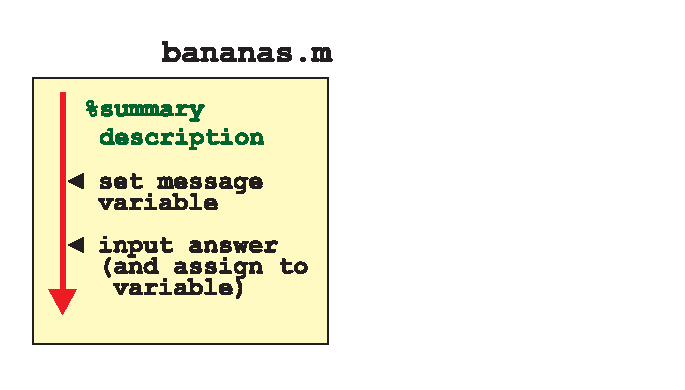
\includegraphics[width=\linewidth]{ch2-bananas.eps}
\caption{Schematic structure of the simple bananas question program.}
\label{fig:ch2-bananas}
\end{marginfigure}

\begin{docspec}
\textcolor[rgb]{0,0.501961,0}{\% === a program to ask whether I like bananas ===
\\\% first -- specify the question 
\\\% (and assign to a variable)}
\\var\_question\textcolor[rgb]{1,0,1}{ = 'Do you like bananas?'};
\textcolor[rgb]{0,0.501961,0}{\\\% now ... ask the question!
\\\% (and store the response in a variable)}
\\var\_answer = input(var\_question,\textcolor[rgb]{1,0,1}{'s'});
\end{docspec}

Run the program thus far. You should see the question displayed, and when you type in an answer and hit \textbf{RETURN}, the program will end. Because your \textit{m-file} is configured as a \textit{script} and not a \textit{function} (see earlier), you can see the variable \texttt{MY\_ANSWER} in the variable list and you can hence check its value -- it should contain a \textit{string} with the answer you gave to the question. Make sure it all works like this so far.\sidenote{HINT: When you type the answer, it appears on the screen immediately adjacent (and untidily) to the end of the question. You can make this look nice(r) by adding a space at the end of the question string you assigned to prompt, e.g. \texttt{PROMPT = 'Do you like bananas? ';}.}

\vspace{1mm}
\noindent\rule{2cm}{0.5pt}
\vspace{2mm}

\noindent OK -- aside from the use of \texttt{input}, there is nothing new here. Yet. The ultimate purpose of the program is to give a reply that depends on the answer given. This is where we are going -- to utilize a \textit{conditional statement} -- depending on whether the answer is 'yes' or not, we are going to display a different message. This is a fundamental programming element -- different code (the \textit{statements} in the \textit{conditional} definition) will execute depending on the value of a \textit{variable} -- in this example, the 'different code' is a different message and the value of the variable is 'yes' or 'no' (or other answer).

Copy your previous \textit{m-file} and give it a new name, so you retain a copy of your previous working program before you start developing it further. Work from this new file.

You are going to add an '\texttt{if ...}' statement to the code (starting on at the end of your current code) to test whether the answer, held in the variable \texttt{MY\_ANSWER}, is equal to '\texttt{yes}'.
In the language of \textbf{MATLAB} syntax (see Box), the \textit{expression} is  whether the string contained in \texttt{MY\_ANSWER} is '\texttt{yes}'. How do we ask \textbf{MATLAB} to compare the value of \texttt{MY\_ANSWER} with '\texttt{yes}'?

Once upon a time, long long ago, \textbf{MATLAB} was simple and helpful and you could write:
\begin{docspec}
if (my\_answer == 'yes')
\\ \ \ [MESSAGE]
\\end
\end{docspec}

\noindent where \texttt{[MESSAGE]} you will later replace by a message that you will display using the \texttt{disp} command that you saw before. (In this stupid example it might be: 'Correct -- they are a great fruit!').
In this (now illegal!) usage, we are trying to ask whether the contents of the \textit{variable} \texttt{my\_answer}, are equivalent (the \texttt{==}) to the string \texttt{'yes'}.

\marginnote[-1.0in]{\begin{mdframed}[backgroundcolor=gray!10, roundcorner=10pt,leftmargin=1, rightmargin=1, innerleftmargin=5, innerrightmargin=5, innertopmargin=5,innerbottommargin=5, outerlinewidth=1, linecolor=light-gray]
\docenvdef{strcmp}
\\For once, the \textbf{MATLAB} help explanation is relatively simple and straightforward:

\textsf{tf = strcmp(s1,s2) compares s1 and s2 and returns 1 (true) if the two are identical. Otherwise, strcmp returns 0 (false).}

Which is pretty well much how we expected asking: \texttt{s1 == s2} to pan out.
\\(In \textbf{MATLAB} \textbf{help} -- \texttt{tf}, the variable name used in the example, is short for 'true-false'.)
\end{mdframed}}

Life is no longer this simple. \textbf{MATLAB} is going to make us use the function \docenv{strcmp} (see Box). In using \docenv{strcmp} we might break things down into 2 steps -- the first comparing the 2 strings (\texttt{MY\_ANSWER} and '\texttt{yes}') and returning to us a value of \textit{true} or \textit{false} that we will store in a new variable. In the second step, we'll ask the conditional to act on the value of the variable. The code will now look like this:
\begin{docspec}
COMPARISON\_RESULT = strcmp(MY\_ANSWER, 'yes');
\\if COMPARISON\_RESULT
\\ \ \ [MESSAGE]
\\end
\end{docspec}

Or, we could have made this more compact:
\begin{docspec}
if strcmp(MY\_ANSWER, 'yes')
\\ \ \ [MESSAGE]
\\end
\end{docspec}

Your code should now comprise something like the 3-5 or so lines from before (comment, define question, get input) followed by 4 lines of code of the conditional structure, comprising: the \texttt{strcmp} function, the \texttt{if ...}, use of \texttt{disp} to display a message, and lastly, \texttt{end}. The structure should look like Figure \ref{fig:ch2-bananas2}\sidenote[][-1.5in]{The red triangle denotes a branch point, where the code can go in different directions depending on the result of the \textit{conditional}. In this example -- there is only one branch, corresponding to the answer being 'yes'.} or if you assign the message to a 2nd variable, like Figure \ref{fig:ch2-bananas3}. A complete example program ... to help you follow all the above, would look like\sidenote[][-1.0in]{Note the \uline{indentation} of the contents of the \texttt{if ... end} structure. This is very common programming practice. You can make \textbf{MATLAB} do this for you by selecting a single line, or highlighting a block of lines, and clicking on the \texttt{Indent} icon in the code editor.}: 

\newpage

\begin{marginfigure}[0.0in]
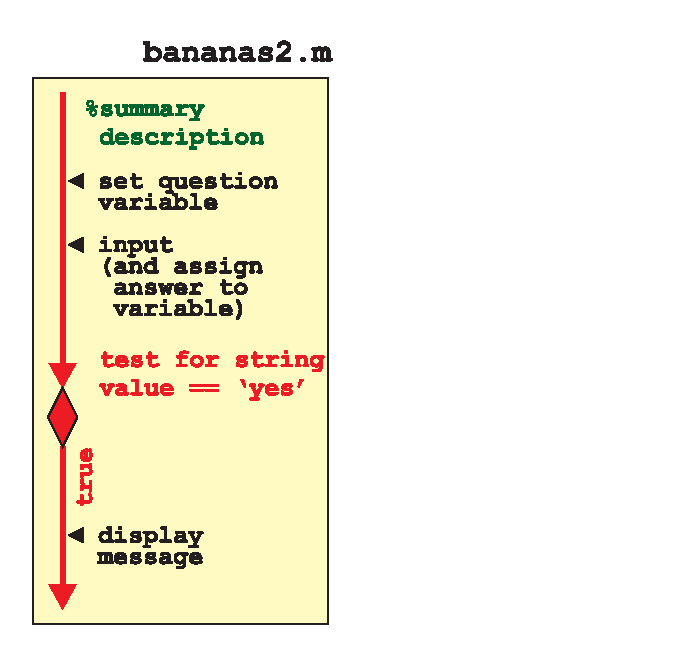
\includegraphics[width=\linewidth]{ch2-bananas2.eps}
\caption{Schematic structure of the extended bananas question program.}
\label{fig:ch2-bananas2}
\end{marginfigure}

\begin{docspec}
\textcolor[rgb]{0,0.501961,0}{\% === a program to ask whether I like bananas ===
\\\% === (and now give an answer!) =================
\\\% first -- specify the question 
\\\% (and assign the string to a variable)}
\\var\_question = \textcolor[rgb]{1,0,1}{'Do you like bananas?'};
\textcolor[rgb]{0,0.501961,0}{\\\% second -- specify the response 
\\\% (and assign the response string to a variable)}
\\var\_response = \textcolor[rgb]{1,0,1}{'Me too! OMG I could die!'};
\textcolor[rgb]{0,0.501961,0}{\\\% now ... ask the question!
\\\% (and store the response in a variable)}
\\var\_answer = input(var\_question,\textcolor[rgb]{1,0,1}{'s'});
\textcolor[rgb]{0,0.501961,0}{\\\% test the answer ... and reply if 'yes'}
\\\textcolor{blue}{if} strcmp(var\_answer, \textcolor[rgb]{1,0,1}{'yes'})
\\ \ \ \ disp(var\_response);
\\\textcolor{blue}{end}
\end{docspec}

\begin{marginfigure}[-0.0in]
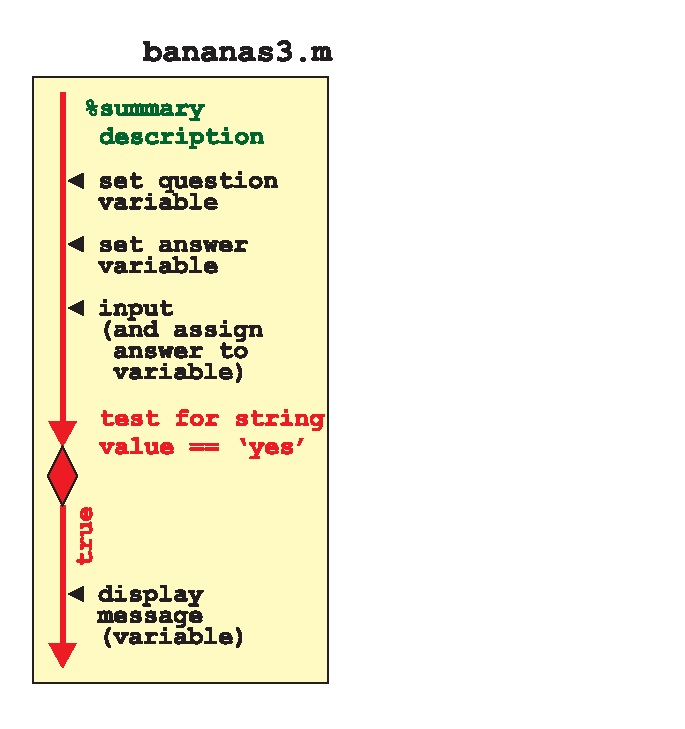
\includegraphics[width=\linewidth]{ch2-bananas3.eps}
\caption{A slight variant on the schematic structure of the extended bananas question program.}
\label{fig:ch2-bananas3}
\end{marginfigure}

\noindent(Please -- do not just copy-paste the code ... write your own version of the code and only use this code as a guide.)

Re-run (after saving) the program and confirm that it works (asking whether you like bananas and if you answer 'yes', tells you 'Correct -- they are a great fruit!'). If not -- time to de-bug! Note that if you tested the code in two stages, any bug at this point is only in the conditional structure. Start by double-checking the syntax required for the \texttt{if ...} structure. You could also try commenting out the message line and re-running.

You can also turn this around, and test for an answer that is not 'no' (the \(\sim\) is making the test, not 'no'), i.e.

\begin{docspec}
if \(\sim\)strcmp(MY\_ANSWER, 'no')
\\ \ \ [MESSAGE]
\\end
\end{docspec}

\noindent Now you are asking whether the answer is something other than 'no' (which might be 'yes', but not necessarily so) -- in the logical construct -- whether the (string) contents of \texttt{answer} are not equivalent to 'no'.

\vspace{1mm}
\noindent\rule{2cm}{0.5pt}
\vspace{2mm}

\noindent Next, you might display an alternative message is the answer is not 'yes'. Refer to \textbf{help} / the margin Box on if ... and note that you can extent the structure with an \texttt{else} which would be followed by a line displaying the alternative message (e.g. 'Then you need to get a life, apple-lover.')\sidenote[][-0.75in]{And then the line with \texttt{end} after that -- follow the prescribed structure *exactly*.}.


Copy your previous \textit{m-file} and give it a new name, so you retain a copy of your previous working program before you start developing it further. Work from this new file.

Try this first -- extend you program with an \texttt{else} line and then a an alternative message. The structure should now look like Figure \ref{fig:ch2-bananas4} and the code like:

\begin{marginfigure}[-0.25in]
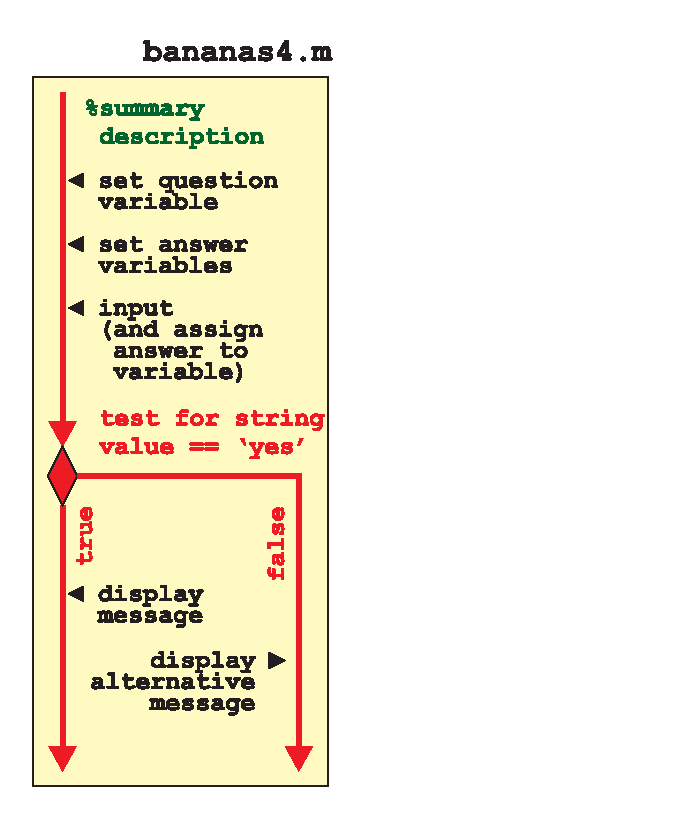
\includegraphics[width=\linewidth]{ch2-bananas4.eps}
\caption{Schematic of the bananas program using the \texttt{if ... else ...} construct (and displaying alternative messages).}
\label{fig:ch2-bananas4}
\end{marginfigure}

\begin{docspec}
if strcmp(MY\_ANSWER, 'yes')
\\ \ \ [MESSAGE1]
\\else
\\ \ \ [MESSAGE2]
\\end
\end{docspec}

Finally -- you could extend this example further and tackle the situation of there being 3 possible answers -- 'yes', 'no', and ... 'I don't know' (or any other answer).
Now the basic structure becomes
\begin{docspec}
if strcmp(MY\_ANSWER, 'yes')
\\ \ \ [MESSAGE1]
\\elseif strcmp(MY\_ANSWER, 'no')
\\ \ \ [MESSAGE2]
\\else
\\ \ \ [MESSAGE3]
\\end
\end{docspec}
\noindent Here -- we are now adding an \texttt{elseif ... }line (followed by its specific message) (and see Box/\textbf{help}). 

Try this extension to your program and test it fully -- inputting a 'yes', a 'no', and some other answer, and confirming that you get the correct message displayed.

\vspace{1mm}
\noindent\rule{4cm}{0.5pt}

\newthought{Continuing to beat this same tired example to death ...} what if some wise-crack answered 'YES' rather than 'yes'?\sidenote{This goes to the heart of all software testing -- what if the user does something you were not expecting? Hence why all software undergoes extensive testing by user or people who did not test it. Sometimes there are pre-releases ('alpha' or 'beta' versions or simple 'pre-release') of software to all or specific parts of the user community, precisely to provide feedback, find bugs, and see whether they can break it ...} One could write:
\begin{docspec}
if strcmp(MY\_ANSWER, 'yes')
\\ \ \ [MESSAGE 1]
\\elseif strcmp(MY\_ANSWER, 'YES')
\\ \ \ [MESSAGE 1]
\\end
\end{docspec}
This will work, but you might note that you have had to exactly duplicate the MESSAGE line. If instead of displaying a simple message, a complex calculation was carried out -- all the lines of the code following the \texttt{if ...} would have to be exactly duplicated after the \texttt{elseif ...} . While it might seem trivial to simply copy-paste the required lines, this is\sidenote{Note quite in the same way that driving down a mountain highway with your eyes shut or hungry sharks are dangerous.} dangerous -- if the first set of lines are ever changed (due to a bug-fix or simple further development of the code), the same changes MUST\ then be exactly duplicated in each and every instance, or the code will not longer work correctly. This is *very* easy to forget to do, particularly for extensive code or code that you have not looked at for ... years. Code duplication also makes the overall code unnecessarily long (and hence harder to look through).

Instead, we can nest statements containing relational operators. What does this mean? Well, in the example of the answer being 'yes' or 'YES', logically, what we want is:

\begin{itemize}[noitemsep]
\setlength{\itemindent}{.2in}
\item[] (1) the contents of \texttt{answer} is equivalent to 'yes'
\item[] \ \ \ \ \ OR
\item[] (2) the contents of \texttt{answer} is equivalent to 'YES'
\end{itemize}
In code, this is written:
\begin{docspec}
strcmp(answer, 'yes') || strcmp(answer, 'YES')
\end{docspec}

Make sure you are happy with what this means (it is pretty well much exactly as it looks == logic).

So -- go modify your code to allow for a 'YES' or a 'yes'. Hell, try allowing for  a 'Y' or a 'y' as well.\sidenote{Sort of for this reason and that there are many different ways of writing 'yes', software often requires you to answer 'yes' in a restricted number of ways -- this restriction is made clear as part of the message that asks the question. Common is to restrict the answer to 'Y' or 'y'.} (You could extend it to 'no' also but I think you get the point ...) Be careful with all the nested parentheses -- an source of mistakes/bugs. You might write it like this, for example: 

\begin{docspec}
if (strcmp(answer, 'yes') || strcmp(answer, 'YES'))
\end{docspec}

\vspace{1mm}
\noindent\rule{4cm}{0.5pt}

\newthought{A non-text and non-fruit related example. Almost.}

How many bananas could you eat in a day? I bet it is less than ten. We'll let the computer ask and if the answer is 10 or more, you (the computer) replies: 'liar!'.\sidenote{This example is even more stupid than the last one. But no more stupid than in any computer programming textbook and it will at least demonstrate a subtly different usage of \texttt{if ...}.}

The basic code is very similar to before. Create a new \textit{m-file}, add a comment line, define your question ('How many bananas do you think you could you eat in a single day?') and then get \textbf{MATLAB} to ask it and pass back whatever is entered in at the command line. 

The only difference at this point -- refer to the usage of \texttt{input} (see earlier Box) -- is that we want a number input rather than a string. So instead of:
\begin{docspec}
MY\_ANSWER = input(MY\_QUESTION,'s');
\end{docspec}
where \textbf{MATLAB} is going to treat whatever you enter as a \textit{string}, we have:
\begin{docspec}
N\_BANANAS = input(MY\_QUESTION);
\end{docspec}
where \textbf{MATLAB} is going to treat whatever you enter as a \textit{number}.

In the if statement, we now want to test whether the value of \texttt{N\_BANANAS} is greater or equal to 10 (or equivalently, greater than 9), i.e.
\begin{docspec}
if (N\_BANANAS >= 10)
\\ \ \ \ [MESSAGE1]
\\else
\\ \ \ \ [MESSAGE2]
\\end
\end{docspec}
or equivalently:
\begin{docspec}
if (N\_BANANAS > 9)
\\ \ \ \ [MESSAGE1]
\\else
\\ \ \ \ [MESSAGE2]
\\end
\end{docspec}

Write this code and get it going. Start with a new blank \textit{script} \textit{m-file}. Your code will look almost identical to previously, except for the different usage of \texttt{input}, and the form of the conditional.

Feel free to switch fruit / fruit consumption threshold, question/answers, or whatever.

%------------------------------------------------

\subsection{\texttt{switch ...}}

A slightly less commonly used alternative to \texttt{if ...} is:

\vspace{1mm}
\texttt{switch ... case ...} 
\vspace{1mm}

\noindent and is helpful in the case of multiple possible correct answers and/or multiple different answers.

\marginnote[-0.75in]{\begin{mdframed}[backgroundcolor=gray!10, roundcorner=10pt,leftmargin=1, rightmargin=1, innerleftmargin=5, innerrightmargin=5, innertopmargin=5,innerbottommargin=5, outerlinewidth=1, linecolor=gray!10]

\textbf{Conditional Statements (2)}
\\The other main \textit{conditional} statement is: \docenvdef{switch ... case ... end}
\\The basic \texttt{switch} structure is:
\begin{docspecmargin}
switch VARIABLE
\\ \ \ \ case VALUE(s)
\\ \ \ \ \ \ \ STATEMENT(s)
\\end
\end{docspecmargin}
which deviates rather from how \textbf{MATLAB} describes it, but this makes more sense to me (and hopefully to you). Here, \texttt{VARIABLE} is a variable and it is compared with one or more \texttt{VALUE(s)}. If the value of \texttt{VARIABLE} matches that of the \texttt{VALUE(s)}, then \texttt{STATEMENT(s)} are executed.

A common variant adds a default set of \texttt{STATEMENT(s)} to be executed if the value of \texttt{VARIABLE} does not match any of the \texttt{VALUE(s)}, e.g.
\begin{docspecmargin}
switch VARIABLE
\\ \ \ \ case VALUE(s)
\\ \ \ \ \ \ \ STATEMENT(s)
\\ \ \ \ otherwise
\\ \ \ \ \ \ \ STATEMENT(s)
\\end
\end{docspecmargin}

You can also have multiple case possibilities:
\begin{docspecmargin}
switch VARIABLE
\\ \ \ \ case VALUE(s)
\\ \ \ \ \ \ \ STATEMENT(s)
\\ \ \ \ case VALUE(s)
\\ \ \ \ \ \ \ STATEMENT(s)
\\ \ \ \ otherwise
\\ \ \ \ \ \ \ STATEMENT(s)
\\end
\end{docspecmargin}

\end{mdframed}}

For instance, and back to the ... fruit ... Consider the situation in which you want the same answer for multiple different kinds of fruit. Trying to code up the program that would give you 'A great fruit!' for any of 'banana', 'kiwi', 'apple', 'pineapple', and 'cucumber' (yes they are technically fruit -- \textbf{Google} it), you will find either that you have many lines of code and many duplicated lines of the same message, or a very long line after \texttt{if ...} with loads of \texttt{strcmp} and ORs (\texttt{||}).

Using \texttt{switch ... case ...} the code might instead look like:
 
\begin{docspecmargin}
switch MY\_ANSWER
\\ \ \ \ case \{'banana', 'kiwi', 'apple', 'pineapple', and 'cucumber'\}
\\ \ \ \ \ \ \ disp('A great fruit!')
\\ \ \ \ otherwise
\\ \ \ \ \ \ \ disp('yuck!')
\\end
\end{docspecmargin}

\noindent where \texttt{MY\_ANSWER} is the variable containing the name of a fruit entered in, in response to input, e.g.
\begin{docspec}
MY\_ANSWER = input('What is your favourite fruit?,'s');
\end{docspec}

Note that for a list of multiple possible values, \textbf{MATLAB} requires the list after \texttt{case} to be encased in curly brackets: \texttt{\{\}}. For a single answer, it would just be:
\begin{docspec}
\ \ \ case 'banana'  
\end{docspec}
for a string, and for a number:
\begin{docspec}
\ \ \ case 10  
\end{docspec}

\vspace{1mm}
\noindent\rule{4cm}{0.5pt}
\vspace{1mm}

\noindent Try re-formulating one of your earlier yes/no \texttt{if} questions in the form of a \texttt{switch ... case ...} code structure, with multiple possibilities for the form of e.g. a 'yes' dealt with by:

\vspace{-4mm}
\begin{docspec}
\\ \ \ \ case \{'YES', 'yes', 'Y', 'y'\}
\end{docspec}

%================================================

\newpage

%================================================

\section{Loops '101'}

%------------------------------------------------

\marginnote{\begin{mdframed}[backgroundcolor=light-gray, roundcorner=10pt,leftmargin=1, rightmargin=1, innerleftmargin=5, innerrightmargin=5, innertopmargin=5,innerbottommargin=5, outerlinewidth=1, linecolor=light-gray]
\textbf{\textit{loops} in \textbf{MATLAB}}

\docenvdef{for}
\\The basic \texttt{for ... end} structure is:
\begin{docspecmargin}
for n = VAL1:VAL2
\\ \ \ \ CODE
\\end
\end{docspecmargin}
\noindent where \texttt{VAL1} and \texttt{VAL2} are the limits that n will count between (starting at \texttt{VAL1} and ending at \texttt{VAL2}), meaning that \texttt{STATEMENT(S)} will be executed \texttt{(VAL2-VAL1)+1} times in total. \texttt{STATEMENT(S)} can be one or more lines of code, that will all be executed on each and every cycle of the loop.
\\The loop need not count in increments of one (1), the default, e.g.:
\begin{docspecmargin}
for n = VAL1:INC:VAL2
\\ \ \ \ CODE
\\end
\end{docspecmargin}
counts with an increment of \texttt{INC}. It is also possible to count down (a negative value of \texttt{INC}).

\docenvdef{while}
\\The basic structure is similar to that for \texttt{for ... end}:
\begin{docspecmargin}
while STATEMENT (TRUE)
\\ \ \ \ CODE
\\end
\end{docspecmargin}
\texttt{while} differs from \texttt{if} in that there are no alternative branches of code that can be executed. The \texttt{while ... end} loop cycles and \texttt{CODE} continued to be executed (for ever) until the \texttt{STATEMENT} is evaluated to be \texttt{false}.
\end{mdframed}}

The next main program construct that you are going to see is the \textit{loop}.
 There are a number of different forms of this in \textbf{MATLAB} (see \textit{loops} Box)  (and also in other programming languages), but the basic premise is the same -- a designated block of code (one of more lines of code\sidenote{It is possible to for the block of code to be only a fragment of a single line and hence the entire \textit{loop} plus code block, to be written on a single line.}), is repeated, until some condition is met. That condition might be something as simple as a count having been reached, e.g. the block of code is always executed  \textit{n} times, or the condition might be slightly more complex and involve a \textit{conditional statement} (see later). Will explore a very basic loop though an example, almost as contrived as for conditionals :o)

%------------------------------------------------

\subsection{\texttt{for ...}}

In this subsection we'll start with a very straight-forward and somewhat abstracted usage of \texttt{for ...}, which hopefully will get you in the mood for \textit{loops}. Then we'll go through some slightly more problem-focused examples.

\vspace{1mm}
\noindent\rule{4cm}{0.5pt}
\vspace{-2mm}

\newthought{Loops Ground Zero}. Basically -- \texttt{for} \textit{loops} cycle through a series of numbers between specific limits, or if you like, 'count' up (or down) through a series of numbers. As the loop counts (cycles), it allows you to execute some code, so for each count (or cycle), the (same) block of code is executed. We'll worry about what you might 'do'\sidenote{Note intentionally a joke. Actually, this is only funny if you know \textbf{FORTRAN}, and even then it is only marginally funny.} (i.e. the code fragment) in a \textit{loop}, later.

Consider, or rather: \textbf{create a new \textit{script} \textsf{m-file}}, and add following  code for a simple loop:
\begin{docspecbold}
for n=1:10
\\end
\end{docspecbold}
Save the file and then run the \textit{script}. What did it do?

I bet you have absolutely no idea! It actually cycled around ten times, counting from \texttt{n=1} through \texttt{n=10}, but you would not know it as there was no code within the loop to do anything and tell you anything about it.\sidenote[][0.125in]{You get one clue -- if you look in the variables \textsf{Workspace window}, you'll see there is a \textit{variable} \texttt{n}, with a value of \texttt{10} -- the last value it was assigned before the \textit{loop} ended.}

There are 2 alternative (but very crude debugging strategies) you could take in order to investigate the behaviour of the code\sidenote{Plus, you could add a \textit{breakpoint} and view the value of n in the \textsf{Workspace window} each cycle around the loop.}:

\begin{enumerate}[noitemsep]
\setlength{\itemindent}{.2in}

\item In the \textbf{MATLAB} \textsf{Editor}, add a \textit{breakpoint} to the \texttt{end} line of the loop. When you run the script, the program stops after the first time around the loop (and as it reaches the \texttt{end} statement). You can now e.g. interrogate the value of \texttt{n} by hovering your mouse pointer over it. You can also \textsf{Continue} (button in the icon bar) the program, and it will then go around the loop once more and then stop again at end. 
\\Typically, there will be one or more lines of code within the loop, and you could create the \textit{breakpoint} at the first line of code (within the loop).

\item Simply add a line \uline{within the loop} with the name of the (counting) variable, e.g.
\begin{docspec}
for n=1:10
\\ \ \ \ n
\\end
\end{docspec}
and it will spit out the value of \texttt{n} each time around the loop.

Or, you could print the value of \texttt{n} 'properly'\sidenote{Although you can get away with just writing:
\begin{docspecmargin}
disp(n)
\end{docspecmargin}
}, e.g.
\begin{docspec}
for n=1:10
\\ \ \ \ disp(n)
\\end
\end{docspec}
You could 'tart this up'\sidenote[][-0.0in]{(make look nicer)} further by creating a string that provides more explicit information back to you, which is when you really need to use \texttt{num2str}, e.g.
\begin{docspec}
for n=1:10
\\ \ \ \ my\_string = ['The value of n is: ' num2str(n)]
\\ \ \ \ disp(my\_string)
\\end
\end{docspec}
or if you are happy with more going on in a single line:
\begin{docspec}
for n=1:10
\\ \ \ \ disp(['The value of n is: ' num2str(n)])
\\end
\end{docspec}
(but they work the same -- check it).

\end{enumerate}

If you are not yet 100\% with \textit{concatenation} -- the '\uline{action of linking things together in a series}' (dictionary definition), what is happening in the line: 

\begin{docspec}
my\_string = ['The value of n is: ' num2str(n)]
\end{docspec}

\noindent is that you are taking the string \texttt{'The value of n is: '}, and the string equivalent of the numerical value of \texttt{n} (created via the use of \texttt{num2str}) and ... joining them together, one (\texttt{num2str(n)}) after the other (\texttt{'The value of n is: '}).

\vspace{1mm}
\noindent\rule{4cm}{0.5pt}
\vspace{-2mm}

\newthought{Loops in action}. So, consider the following (somewhat contrived) problem -- you want to be able to enter a series of numbers and return their sum (although equally one could perform and return all sorts of statistics).\sidenote{Obviously, one way to do this would be to enter the numbers into a file first, use the load function, and calculate the sum.} The basic code is simple and you can try it out by \textbf{first creating a new (\textit{script}) \textsf{m-file}}.

Using the other (numerical input) form of \texttt{input} (see earlier), the code for entering 2 numbers, one after the other, might look like this (although in practice, your code is full of helpful comments, right?):
\begin{docspec}
my\_question\ = 'Please enter a number: ';
\\A = input(my\_question);
\\my\_question = 'Please enter a number: ';
\\B = input(my\_question);
\\disp(['The sum of the numbers is:  ' num2str(A+B)]);
\end{docspec}

The first 4 lines you should be A-OK with, you have seen something very like this before. In the last line, again, 2 strings have been \textit{concatenated} by enclosing \texttt{'The sum of the numbers is:  '} and \texttt{num2str(A+B)} in a pair of brackets \texttt{[]}. The string representing the number sum is itself created by adding \texttt{A} and \texttt{B}, and then converting the resulting number into a string using \texttt{num2str} (see earlier). As always -- if you are happier breaking down the last line into its component parts, e.g.
\begin{docspec}
answer = A+B;
\\answer\_string = num2str(answer);
\\disp(answer\_string);
\end{docspec}
then please do! There is no particular computational penalty in \textbf{MATLAB} for creating as many variables as you like and breaking down code into multiple lines.

So far so good. But what if you wanted 4 numbers summed ...
\begin{docspec}
my\_question = 'Please enter a number: ';
\\A = input(my\_question);
\\my\_question = 'Please enter a number: ';
\\B = input(my\_question);
\\my\_question = 'Please enter a number: ';
\\C = input(my\_question);
\\my\_question = 'Please enter a number: ';
\\D = input(my\_question);
\\disp(['The sum of the numbers is:  ' num2str(A+B+C+D)]);
\end{docspec}

You can see whether this is going -- firstly that you are duplicating more and more lines of code as the number of numbers increases. Secondly, and we'll come to that in a moment -- what if the program does not know \textit{a priori} how many numbers you want to sum? Or do you need to write a program for every single possible number of numbers that you might need to input and process? An impossible and thankless task ...

You can see the code that is being repeated (here for input \texttt{x}):
\begin{docspec}
my\_question = 'Please enter a number: ';
\\x = input(my\_question);
\end{docspec}

If you bothered to read the margin box earlier, you'd known that this is exactly what a \textit{loop} can be used for. We therefore want something of the form:
\begin{docspec}
for n = 1:MAX\_N
\\ \ \ \ my\_question = 'Please enter a number: ';
\\ \ \ \ x = input(my\_question);
\\end
\end{docspec}

\noindent (noting that in your own code, \texttt{MAX\_N}, for instance, could be \texttt{4}).

The easy part is the configuration of the loop -- in the previous example with 4 inputs, we would write:
\begin{docspec}
for n = 1:4
\end{docspec}
and the \textit{loop} with go around 4 times as the counter \texttt{n} counts from 1 to 4 (\texttt{MAX\_N}) in increments of 1 (the default behavior of the \textit{colon operator}). Each time around the \textit{loop} the block of (2 lines of) code is executed and a number is inputted. But what is still missing? Try this (in a new \textsf{m-file}): 
\begin{docspecbold}
for n = 1:4
\\ \ \ \ my\_question = 'Please enter a number: ';
\\ \ \ \ x = input(my\_question);
\\end
\end{docspecbold}
and see if you can see what is going on, or rather, not going on. If you think that it is not working as expected -- try some debugging (i.e. adding one (or more) \texttt{disp} statements within the loop code, \uline{or} add a \textit{breakpoint} within the \textit{loop}). (You should have deduced that what is not going on, is that you are not learning what the sum of all those numbers is.)  

See if you can come up with a solution for how to determine the sum of all the numbers you inputted. (Warning: the spoiler is in the margin.)

\marginnote[-5.875in]{
It should be apparent if you tried it out, that the value of \texttt{x} at the very end of the program, is equal to the last value you entered. In other words, each time you go around the loop you are over-writing the previous entered value and end up with nothing to sum at the end. There are two (or more) possibilities to solve this:
\begin{enumerate}[noitemsep]
\setlength{\itemindent}{.2in}
\item You could keep a \textit{running sum}. This would also avoid having to explicitly calculate a sum at the end, but you would not have saved the numbers as you went an no other stats would be possible.
\\You would do this by adding the inputted value to the existing value, i.e.
\begin{docspecmargin}
x = x + input(prompt);
\end{docspecmargin}
where \texttt{x} is the running total. What this says is: take the current value of \texttt{x}, add the value if the user input, and place the total back into the variable \texttt{x}. 
\\The only problem here ... is that \textbf{MATLAB} does not know what the very first value of x is -- i.e. the value before the loop start and that you then try and add \texttt{input(prompt)} to. The solution is to initialise the value of x before the loop starts, e.g.
\begin{docspecmargin}
x = 0;
\end{docspecmargin}
\item Alternatively, you could add the newly inputted number to the end of an existing vector. In this way, you end up recording all the values that were inputted. e.g.
\begin{docspecmargin}
y = [y input(prompt)];
\end{docspecmargin}
which says take the vector \texttt{y}, and add a further value (\texttt{input(prompt)}) to the end of it. At the end of the program (after the loop has terminated), you have to sum the contents of the vector \texttt{y}.

Or, to break it down:
\begin{docspecmargin}
z = input(prompt);\\
y = [y z];
\end{docspecmargin}
\end{enumerate} 
}

Try out  both of the given alternatives (see margin) (assuming that one of them was not also your solution). Note that you are not given the complete code needed and some further debugging might be needed (but they do both work!).

Two things to be aware of in doing this:

\begin{enumerate}[noitemsep]
\setlength{\itemindent}{.2in}
\vspace{1mm}
\item If you set the maximum number of items quite high and then get bored and need to exit the program -- press the key combination \textsf{Ctrl-C} and \textbf{MATLAB} will exit your program (but leave \textbf{MATLAB} itself still running).
\vspace{1mm}
\item If you run the program a second time and use the \textit{vector} approach (see margin), something very odd starts to happen to the reported sum. This is because there already exists a \textit{vector} with the same name left over from the first time you ran the \textit{script} program. You can solve this (first try it out -- running the program several times in a row to see what happens) either by initializing the vector \texttt{y}, just like you did for \texttt{x} in the 1st solution, i.e.
\begin{docspec}
y = [];
\end{docspec}
(before the loop starts, of course), or you can clear the workspace using \texttt{>> clear all} (clears *all* variables), or clear just the problem variable (\texttt{y}) that will end up growing and growing and growing ... (\texttt{>> clear y}).
\\You could also add \texttt{clear all} to the very start of your \textit{script} \textsf{m-file}.
\end{enumerate}

\vspace{-1mm}
\noindent\rule{4cm}{0.5pt}
\vspace{2mm}

\noindent A different and simpler way of looking at creating a running sum, or in the case below, incrementing the value of a variable within the loop, is to consider creating an explicit counting variable, sperate from the loop counter. Recall:

\begin{docspec}
for n = 1:10\\
end
\end{docspec}

\noindent will simply loop around 10 times, as the \textit{loop} counter \texttt{n} is repeatedly incremented by 1 (the default increment of the colon operator), until it reaches a value of 10.

Create a new \textsf{m-file} and enter the following code:

\begin{docspec}
\textbf{m = 0;\\
for n = 1:10\\
\ \ \ m = m+1;\\
end}
\end{docspec}

\noindent What do you expect to happen to the value of m? Add some \texttt{disp} statements and print out the values of \texttt{n} and \texttt{m} (from within the \textit{loop}), each time around the \textit{loop}, or add one or more \textit{breakpoints} in the \textbf{MATLAB} code editor. Was this what you expected? Why?

As abstracted and odd as it might seem now, later, this will all be important to understand. Please make sure you do!

\marginnote{Note that you \uline{should not} re-use the same variable name \texttt{n} that you use for the \textit{loop} counter, as in something like:
\begin{docspecmargin}
n = 0;\\
for n = 1:10\\
\ \ \ n = n + 10;\\
end
\end{docspecmargin}
Why? (Try it and see, even.)}

%------------------------------------------------

\subsection{Other loop configurations and usages}

In the previous examples, the \textit{loop} limits were fixed in the program itself -- you'd have to edit the \textit{script} code and re-save the file in order to be able to input and sum a different number of values. You could create a more flexible program by making the \textsf{m-file} a \textit{function} rather than a \textit{script}.\sidenote{There are other ways of adding flexibility to the loop count that we'll see shortly.} 

The idea here is to create a \textit{function} that takes a single input. This input will be the maximum \textit{loop} count. If the input variable was called \texttt{max\_count}, then the \textit{loop} structure would now look like:
\begin{docspec}
for n = 1:max\_count
\\ \ \ \ my\_question = 'Please enter a number: ';
\\ \ \ \ x = input(my\_question);
\\end
\end{docspec}
and the all-important \textit{function} header line would be:
\begin{docspec}
function [] = function\_sum(max\_count)
\end{docspec}

Referring to the previous lessons on \textit{functions} (as well as \textsf{help} if need be), create a \textit{function} that when you call it, e.g. like:
\begin{docspec}
>> function\_sum(5)
\end{docspec}
will request 5 inputs in turn, and at the end, display the sum.\sidenote{So in addition to the code fragment given, you need to define (at the top) and then end (at the bottom) a \textit{function}, you need to create a running sum, and then after the \textit{loop} finishes, display the sum.}

Also create a variant of this \textit{function}, and have it return the sum, rather than display it. i.e. this \textit{function} will now take as input, the number of numbers you wish to input, but will now return the sum of those numbers as a single output.

Alternatively, you could write your program as a \textit{script} and before the loop starts,  ask for the number of values to be entered, passing this to the variable \texttt{max\_count}, with the loop then looking exactly like the above. In both cases you are substituting a fixed number (e.g. 4) for a variable that might contain any number.

\vspace{1mm}
\noindent\rule{4cm}{0.5pt}
\vspace{2mm}

\noindent Finally, in addition to a flexible \textit{loop} count maximum limit, the value of the increment in the count each time around the loop need not be one and it also need not start from 1. For example:
\begin{docspec}
for n = 10:10:100
\\ \ \ \ ...
\\end
\end{docspec}
is  equivalent in terms of the number of iterations carried out to
\begin{docspec}
for n = 1:1:10
\\ \ \ \ ...
\\end
\end{docspec}
and which is the same as the default behavior of the colon operator:
\begin{docspec}
for n = 1:10
\\ \ \ \ ...
\\end
\end{docspec}
The value of  the loop counter \texttt{n} simply differs by a factor of 10 at every iteration between the top and bottom two versions.

\newpage 

%------------------------------------------------

\subsection{Fun(!) worked examples}

(Only one example to date. And not necessarily even that fun.)

\vspace{1mm}
\noindent\rule{4cm}{0.5pt}
\vspace{-2mm}

\newthought{\textit{Loops}, camera, action!}\footnote{\textcolor{red}{\textbf{Example codes provided}}}\footnote{(at end of text)} (A more colorful example of \textit{loops} in action.) What we are going to do is (load and) plot a sequence of monthly data-sets and put them together to create a movie (animated graphic) to illustrate the seasonality of temperature in global climate. You will hopefully thereby better appreciate the value of constructs such as \textit{loops} in computer programming in saving you a whole bunch of effort and needless duplication of code. (Equally, you might not have wanted a movie as the end result, but simply a number of plots, all identical except in the specific array of data they were plotted from.)

First download all the monthly global surface temperature data-files on the  course webpage (there are 12 files to download)\sidenote{In scripting, it is also possible to automate downloading files from the internet.}. Then you are going to want to plot them all ... which would get desperately tedious if you had to do this at the command line 12 times. Think how much more of your life you would be wasting if the data were weekly. Or monthly data for 1972 through 2003, some 372 separate data-files ... You would never have time to go get a coffee ever again(?) So we are going to use a \textit{loop}.

To make an animation, we need to make a series of frames, with each one being a different monthly temperature plot (in sequence; Jan through Dec). The files are rather conveniently named: \texttt{temp1.tsv}, \texttt{temp2.tsv}, ... \texttt{temp12.tsv}\sidenote{Don't worry about the \texttt{.tsv} file extension -- the file format is plain old text (ASCII) and could have instead been \texttt{.txt}.}. We should start by loading this little lot in. For example, at the command line, to load in the the first file we could write:
\begin{docspecbold}
>> temp = load('temp1.tsv');
\end{docspecbold}
or equally:
\begin{docspec}
>> temp(:,:) = load('temp1.tsv');
\end{docspec}
Then for the 2nd file:
\begin{docspecbold}
>> temp = load('temp2.tsv');
\end{docspecbold}
and the third ...
\begin{docspecbold}
>> temp = load('temp3.tsv');
\end{docspecbold}
...

This is something that a \textit{loop} could be used for while you go off for a coffee. So this is what we are going to do -- use a \textit{loop} to load in all of the files in turn.

\textbf{Create a new \textit{script} \textsf{m-file}.} Call it ... anything you like\sidenote{\texttt{bob\_the\_builder.m} counts as 'anything you like', but that looks pretty lame and it certainly won't help you remember what the script does if you came back to it sometime in the future.}. However, as well as appropriately naming your \textit{script} file, add a \textit{comment} on the first line of the file as a reminder to yourself of what it is going to do. (If you get totally confused as to what should be going into the program and where -- refer to the 'answers' for this section at the back of the book.)

We first need to construct the \textit{loop} framework. We'll call the month number counter variable, \texttt{month}. Create a \texttt{for} \textit{loop} (with nothing in it yet) with \texttt{month} (as the counting variable) going from \texttt{1} to \texttt{12}.\sidenote{Don't forget to suitably comment what it is that the \textit{loop} does with a line (or even 2, but don't write a whole essay) beginning with a \%.} Refer to the course text (this document!), and/or the \textbf{MATLAB}  documentation, and/or the entirety of the internet, if necessary. The syntax (and examples) is described in full under \texttt{>> help for}. Save the script (\textsf{m-file}) and run it\sidenote{Typing: the \texttt{m-file} filename without the extension.}. What happens? Can you tell?

One way of following what is going on as \textbf{MATLAB} executes the commands within a script is to explicitly request that it tells you how it is getting on. You can use the function \docenv{disp} to help you follow what the program is doing (this is Old School debugging\sidenote{You can also add a \textit{breakpoint} within the \textit{loop} and thus can cycle through the \textit{loops} one-by-one, thereby being able to check the status of the variables within the loop and how they change from iteration to iteration.}). Within the loop (anywhere!), add the following line:
\begin{docspecbold}
disp(month)
\end{docspecbold}

\noindent and then save and re-run the \textit{script}. Now you can see how the loop progresses. This sort of thing can be useful in helping to \textit{debug} a program -- it allows you to follow a program's progress, and if the program (or \textbf{MATLAB} script) crashes, then at least you will know at what loop count this happened at, even if you are not given any more useful information by \textbf{MATLAB}. Only when you are happy that you have constructed a \textit{loop} that goes around and around 12 times with the variable \texttt{month} counting up from 1 to 12; comment out (\texttt{\textcolor[rgb]{0,0.501961,0}{\%}}) the printing (\texttt{disp}) line\sidenote{Note that by commenting out a line rather than completely deleting it, if you want to print out the loop count in the future, all you have to do is to un-comment the line, rather than type in the command all over again. This can be really useful if your debug command is long, or particularly if you have a whole series of lines that are required to report the information you want to know.} (unless you have grown rather attached to it) and move on.

We can construct filenames to load in by:
\begin{enumerate}[noitemsep]
\setlength{\itemindent}{.2in}
\item Forming a complete filename by \textit{concatenating} sperate strings. For example: 
\begin{docspec}
>> filename = ['temp' '1' '.tsv']
\end{docspec}
\noindent will create the filename  out of 3 components parts -- a common elements of all the filenames (\texttt{'temp'}), the number of the month (\texttt{'1'}), and the file extension (\texttt{'.tsv'}). 
\vspace{1mm}
\item Converting a number value of a (count) variable to a string (the \docenv{num2str} function), so instead of hard-coding in the string representing a number (\texttt{1} in this example), you convert from the value of a counter, e.g. \texttt{num2str(month)}.
\end{enumerate}

\marginnote[-1.0in]{\begin{mdframed}[backgroundcolor=gray!10, roundcorner=10pt,leftmargin=1, rightmargin=1, innerleftmargin=5, innerrightmargin=5, innertopmargin=5,innerbottommargin=5, outerlinewidth=1, linecolor=gray!10]
\docenvdef{num2str}
\\Converts a number to a \textit{string} (\texttt{s}), e.g.
\begin{docspecmargin}
s = num2str(N)
\end{docspecmargin}
where \texttt{N} is any number type variable.
\\\texttt{num2str} is useful in adding specific captions to plots (with caption text based on the value of a numerical variable) and in creating automated strings (e.g. filenames) within a loop.
\end{mdframed}}

This is where the role of the loop counter  (stored in the variable \texttt{month}) comes in. Each time around the loop,  the value of  variable \texttt{month} is the number of the month. All you have to do is to convert this value to a  \textit{string} and thereby automatically generate the correct month's filename each time (as per above).

Now add the following within the \textit{loop} in your script;
\begin{docspecbold}
filename = ['temp' num2str(month) '.tsv'];
\end{docspecbold}
and after it (still within the \textit{loop}), add some some debugging\sidenote{Or you can make use of a \textbf{breakpoint}.}:
\begin{docspecbold}
disp(filename)
\end{docspecbold}

\noindent just to confirm that appropriate filenames are being generated.

Save and run the \textit{script}. Satisfy yourself that you know what it is doing. Can you see that you are now automatically generating all the 12 filenames in sequence? And this only takes 3 lines of code total (not including the debugging line), compared with 12 lines if you had to write down all the 12 file names long-hand.
 
Now \textit{comment out} (or delete) the \texttt{disp(filename)} line, and add a new line to load in each dataset from the filename that is constructed each time the loop goes around.\sidenote[][-1.0in]{Remember that the load line goes inside the loop. (Why? Try writing it outside the loop (at the end) and see what happens if you like.)} e.g.\footnote{Alternatively, you could store all the data slices as you load them in and  rather than specifying the 1st, then 2nd, etc layer of the 3D array, here we are specifying the layer with an index equal to the contents (or value) of \texttt{month}, which, if you remember, counts up from 1 to 12 in the \textit{loop}.
\begin{docspecmargin}
temp(:,:,month) = ... load(filename,'-ascii');
\end{docspecmargin}
If youn run this coding variant and take a look at the \textsf{Workspace window} -- note that you have an array (\texttt{temp}) that has size 94\(\times\)192\(\times\)12.
}:
\begin{docspecbold}
temp(:,:) = load(filename);
\end{docspecbold}

\noindent Note that rather than specifying the filename explicitly in the load command, you are now passing the string contained in the variable \texttt{filename}. (Hopefully on the previous line of code within the loop, you have created the string value of \texttt{filename} ...)

\vspace{1mm}
\noindent\rule{4cm}{0.5pt}
\vspace{2mm}

\noindent We'll now add some graphics.

\begin{marginfigure}[0.5in]
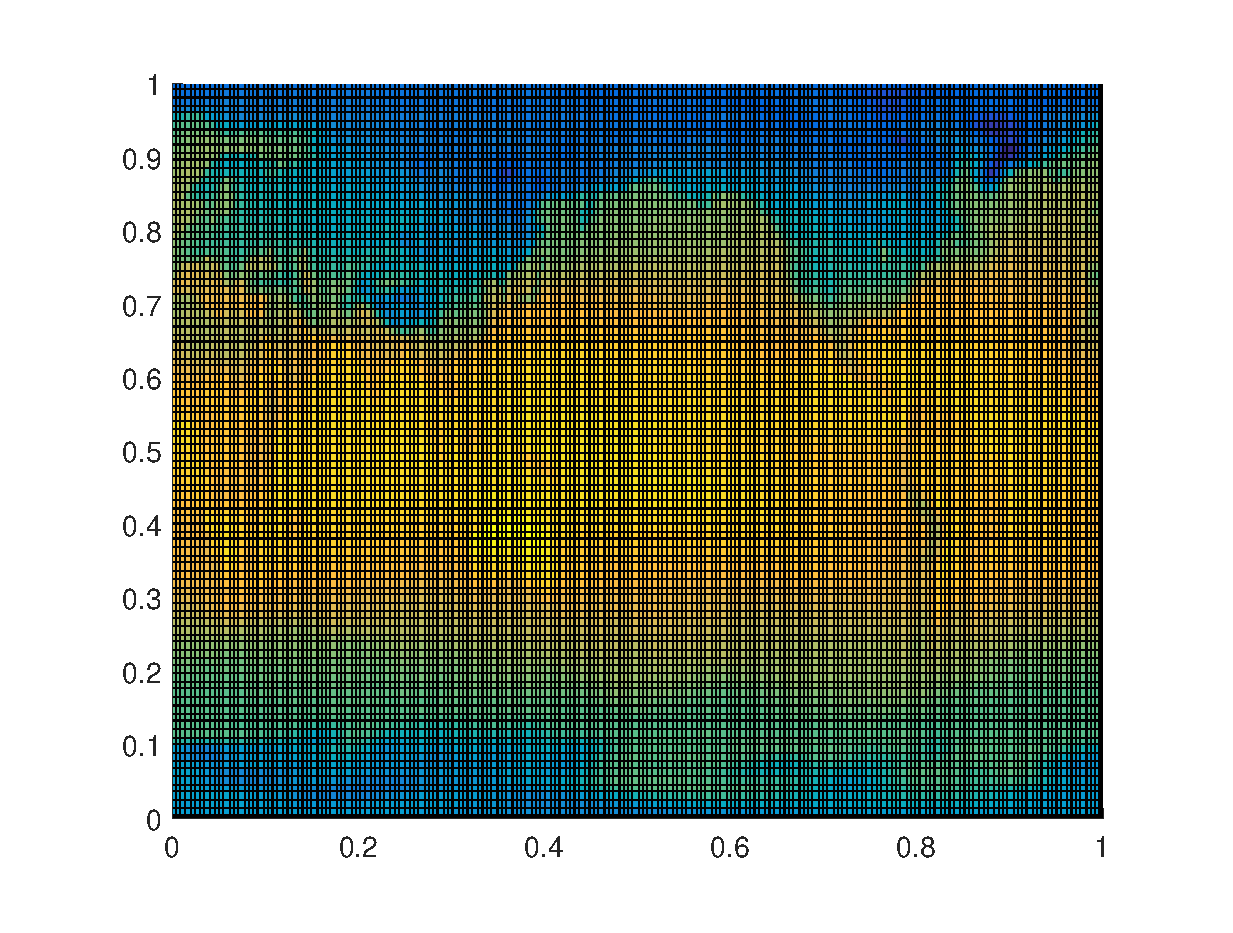
\includegraphics[width=\linewidth]{ch3-pcolortemp.eps}
\caption{Extremely unappealing blocky plot of Earth surface temperature (who cares with month? -- the graphics are too poor to matter ...).}
\label{fig:ch3-pcolortemp}
\end{marginfigure}

At the end of (but still within) the \textit{loop} (i.e., before the \textit{loop} has completely finished), create a new \textsf{figure window} and then plot (using \texttt{pcolor}) the monthly temperature data. On the subsequent lines, add the essential labelling stuff (lines after that). All within the loop still. These lines should look something like:
\begin{docspecbold}
figure;
\\pcolor(temp(:,:));
\end{docspecbold}

\noindent (or could be simply written \texttt{pcolor(temp);}) and should produce extremely exciting graphics as in Figure \ref{fig:ch3-pcolortemp}\sidenote[][0.25in]{The 2D graphics will get *much* better later -- one thing at a time!}.

Save and run the \textit{script}. Do you have 12 different temperature plots on the computer screen?\sidenote[][0.0in]{If not, stick you paw up in the air for help ...} Note that if you keep running the program, you'll get 12 more figure windows each time. This is where the \texttt{close all} command comes in useful, and you could add this at the start (or end) of your \textit{script}. Because if you re-run the \textit{script}, you wont then end up with 24 figure windows. And then 36 the time after that, and ... 

Actually, there is  no need to create a new \textsf{figure window} each time -- comment out the command that creates a new \textsf{figure window} (\texttt{figure}). Save and re-run and note the difference. 

\vspace{1mm}
\noindent\rule{4cm}{0.5pt}
\vspace{2mm}

\noindent Finally ... look up \textbf{MATLAB} \texttt{help} on \docenvdef{getframe}. Then go back to your global temperature loading/plotting script and add the following line to your program\sidenote{Where to put the line? Within the loop and after you have plotted the plot.}:
\begin{docspecbold}
M(month) = getframe;
\end{docspecbold}
This lines goes at the very end of the loop (before \texttt{end}), to give you:
\begin{docspec}
for month=1:12\\
\ \ \ filename = [\textcolor[rgb]{1,0,1}{'temp'} num2str(month) \textcolor[rgb]{1,0,1}{'.tsv'}];\\
\ \ \ temp(:,:) = load(filename);\\
\ \ \ pcolor(temp(:,:));\\
\ \ \ M(month) = getframe;\\
end
\end{docspec}

Save and run. When \textbf{MATLAB} is all done, at the command line, type:
\begin{docspecbold}
>> movie(M,5,2)
\end{docspecbold}
and hopefully ... an animation of the progression of monthly surface air temperatures globally, should appear\sidenote{Note that the active Figure window may have disappeared behind some other windows so go rescue it to see what is happening.}.

If you want to play some more, just type \texttt{help movie} -- there are controls for not only the number of times you loop through the complete animation, but also for the numbers of frames per second. But we will revisit this later -- the 2D plotting you have done so far is *very* basic and there is no scale or sane x/y axes. Later we can also add the continental outlines that will help orient you and improve the quality of the graphical output. 

\uline{Before} you move -- go look at your \textit{script} -- is it well commented? Would you be able to tell exactly what it does it by the end of the course? What about next year? Are the \textit{loop} contents indented? It is important that it is commented and laid out adequately.

\vspace{1mm}
\noindent\rule{4cm}{0.5pt}
\vspace{2mm}

\noindent Creating a portable animation format would be useful (i.e. that you could play on a different computer or upload to the internet). There is no longer a convenient \textbf{MATLAB} command to turn the \textbf{MATLAB} format movie (\texttt{M}) into a format you can use elsewhere (there used to be a command called \docenv{movie2avi}, but it has been 'retired' (curse you, Mathworks)). The new/replacement command is \docenvdef{VideoWriter,} which differs mostly in that the animation is now created within the program and the  \textsf{.avi} format animation has its frames added (within the loop) as the graphics are created.

To use the \textbf{MATLAB} \docenv{VideoWriter} \textit{function} to create the animation, you will need the following code (that you should put into a new \textsf{m-file}):
\begin{docspecbold}
\textcolor[rgb]{0,0.501961,0}{\% Prepare the new file.}\\
vidObj = VideoWriter(\textcolor[rgb]{1,0,1}{'my\_animation.avi'});\\
open(vidObj);\\
\textcolor[rgb]{0,0.501961,0}{\% Create an animation.}\\
for month=1:12\\
\ \ \ filename = [\textcolor[rgb]{1,0,1}{'temp'} num2str(month) \textcolor[rgb]{1,0,1}{'.tsv'}];\\
\ \ \ temp = load(filename);\\
\ \ \ pcolor(temp);\\
\ \ \ \textcolor[rgb]{0,0.501961,0}{\% Write each frame to the file.}\\
\ \ \ currFrame = getframe;\\
\ \ \ writeVideo(vidObj,currFrame);\\
end\\
\textcolor[rgb]{0,0.501961,0}{\% Close the file.}\\
close(vidObj);  
\end{docspecbold}

\vspace{1mm}
\noindent\rule{4cm}{0.5pt}
\vspace{2mm}

\noindent Note that if we wanted to save all the data in a 3D array, we could also have written:
\begin{docspecbold}
>> temp(:,:,1) = load('temp1.tsv');
\end{docspecbold}
and then for the 2nd month:
\begin{docspecbold}
>> temp(:,:,2) = load('temp2.tsv');
\end{docspecbold}

What you have done here is to load the January 2D (lon-lat) temperature distribution into the 1st 2D layer of the \texttt{temp} array, and then we have gone and created a second 2D layer on top of the first with the February climate data in it. Look at the \textbf{Workspace window} (or type \texttt{size(temp)}) -- you now have a 3D (94\(\times\)192\(\times\)2) array. Fancy! This is your first 3D array -- there is nothing really conceptually different from the 2D arrays that you have already been using, we simply have a 3rd index for the third dimension -- if it helps, \uline{you can think of a 3D array as being indexed by: row, column, layer}. 

You could go on and load in the March, April, etc data in a similar fashion, but you should be able to see a pattern forming here -- each filename differs only in the number at the end of its name and this number corresponds not only to the number of the month, but will also correspond to the layer index of the 3D array that you will create.

A loop for this might look like:
\begin{docspec}
for month=1:12\\
\ \ \ filename = [\textcolor[rgb]{1,0,1}{'temp'} num2str(month) \textcolor[rgb]{1,0,1}{'.tsv'}];\\
\ \ \ temp(:,:,month) = load(filename);\\
\ \ \ pcolor(temp(:,:,month));\\
\ \ \ M(month) = getframe;\\
end
\end{docspec}
and at the end, you will have a 3D array -- \texttt{temp} -- containing all the months data.

%================================================

\newpage

%================================================

\section{Loops and conditionals ... together(!)}

%------------------------------------------------

No surprise that you might combine both \textit{loops} and \textit{conditionals} in the same programming structure. In fact, this becomes very powerful and is an extremely common device in programming. But this can all also become confusing ... remember to \uline{indent} your code.

\marginnote[-0.5in]{
\textbf{Indenting code}
\\Just do it (or let \textbf{MATLAB} do it).
Even for a single \textit{loop} or \textit{conditional}, it is way easier to see what code is within the \textit{loop} and what outside it, when the code inside starts several spaces in from the margin.
\\For nested \textit{loops} and \textit{conditionals}, it is even more important to keep (visual) track on what is going on.
\\Note that the indention (or lack of) does not affect the execution of the code (unlike in e.g. \textbf{Python}).
}

%------------------------------------------------

\subsection{\texttt{for ...} and conditionals}

Firstly, one might (rather trivially) use a conditional to decide whether to execute a loop 10 or 100 times, e.g.

\begin{docspec}
my\_string = input('Loop only 10 times (y or n)','s');
\\ if strcmp(my\_string,'y')
\\ \ \ \ for n = 1:10
\\ \ \ \ \ \ \ SOME CODE
\\ \ \ \ end
\\ else
\\ \ \ \ for n = 1:100
\\ \ \ \ \ \ \ SOME CODE
\\ \ \ \ end
\\ end
\end{docspec}

Here, we have a \textit{conditional} structure testing whether the string entered in response to the questions is 'y'. \texttt{If} 'y', then a loop of maximum count 10 executes, if not ('y') (\texttt{else}), then a loop of maximum count 100 executes.

This is a little messy and could be cleaned up and simplified somewhat. For instance -- by replacing the maximum loop count as a variable, whose value is set by the (\textit{conditional}) answer. e.g.

\begin{docspecbold}
my\_string = input('Loop only 10 times (y or n)','s');
\\ \textcolor{blue}{if} strcmp(my\_string,'y')
\\ \ \ \ n\_max = 10;
\\ \textcolor{blue}{else}
\\ \ \ \ n\_max = 100;
\\ \textcolor{blue}{end}
\\ \textcolor{blue}{for} n = 1:n\_max
\\ \ \ \ \textcolor[rgb]{0,0.501961,0}{\%}
\\ \textcolor{blue}{end}
\end{docspecbold}

\textbf{Enter in the second code (or some variant of it) into a new \textit{script} m-file, and explore how it works -- try changing the alternative loop limits, add a line within the loop to \texttt{disp} the value of \texttt{n} and hence confirm that the correct number of iterations of the loop occurs.} Note that you will need to replace \texttt{\textbf{\textcolor[rgb]{0,0.501961,0}{\%}}} with your own line (e.g. using \texttt{disp}) or you could have nothing and leave the comment \textcolor[rgb]{0,0.501961,0}{\%} line in. Remember to add comment lines.

\vspace{1mm}
\noindent\rule{4cm}{0.5pt}
\vspace{2mm}

\noindent Returning to the previous loop example concerning summing a series of numbers entered --  an alternative to (or as well as) a fixed \textit{loop}, or variable and (\textit{function}) parameter passed controlled \textit{loop}, we could specify a near infinite \textit{loop}, but provide a get out of jail free. For example, within the \textit{loop}, we could add a line that asks an additional question: 'Another input (y/n)?' We would test the answer and if no ('n'), exit the \textit{loop} (and report the sum as before). This would look like:
\begin{docspecbold}
\textcolor[rgb]{0,0.501961,0}{\% set up some strings for the 2 questions}
\\my\_question1 = 'Please enter a number: ';
\\my\_question2 = 'Another input (y/n)? ';
\\\textcolor[rgb]{0,0.501961,0}{\% initialize running sum}
\\running\_sum = 0.0;
\\\textcolor[rgb]{0,0.501961,0}{\% START OF LOOP}
\\\textcolor{blue}{for} n = 1:1000000
\\ \ \ \ \textcolor[rgb]{0,0.501961,0}{\% ask for a number}
\\ \ \ \ my\_number = input(my\_question1);
\\ \ \ \ \textcolor[rgb]{0,0.501961,0}{\% update running sum}
\\ \ \ \ running\_sum = running\_sum + my\_number;
\\ \ \ \ \textcolor[rgb]{0,0.501961,0}{\% display running sum}
\\ \ \ \ disp(['sum so far = ' num2str(running\_sum)])
\\ \ \ \ \textcolor[rgb]{0,0.501961,0}{\% ask whether to keep going}
\\ \ \ \ my\_string = input(my\_question2,'s');
\\ \ \ \ \textcolor[rgb]{0,0.501961,0}{\% exit loop if answer is no}
\\ \ \ \ \textcolor{blue}{if} strcmp(my\_string,'n')
\\ \ \ \ \ \ \ \ break
\\ \ \ \ \textcolor{blue}{end}
\\\textcolor{blue}{end}
\\\textcolor[rgb]{0,0.501961,0}{\% END OF LOOP}
\end{docspecbold}

\noindent where \texttt{1000000} in the code is simply chosen as a 'very large number' and one rather larger than the maximum number of numbers you could ever imagine entering\sidenote{There us a better way of doing this, with the \texttt{while} construct, that we'll see shortly.}.

\marginnote[-0.0in]{\begin{mdframed}[backgroundcolor=gray!10, roundcorner=10pt,leftmargin=1, rightmargin=1, innerleftmargin=5, innerrightmargin=5, innertopmargin=5,innerbottommargin=5, outerlinewidth=1, linecolor=light-gray]
\docenvdef{break}
\\Simply -- \docenv{break} terminates the execution of a for or while loop'. And from \textbf{help} a further clarification: 'Statements in the loop after the break statement do not execute.'
\\Slightly more complicated (but not much) in the case of nested loops -- in this case, \texttt{break} exits only the loop in which it occurs.
\end{mdframed}}

The key new command here is \docenv{break}. The way the code works (hopefully!) is that towards the end of the \textit{loop}, the 'another input' question is asked -- if no further input is required, the loop exits via the \texttt{break} command. Remember  that now we have \textit{loops} and \textit{conditionals} nested together, it helps even more to \textit{indent} the code as per illustrated in the given code fragment\sidenote{\textbf{MATLAB} will do this for you if you click on the Indent icon. It will also indent the code as far as it reasonably can, as you type.}. Also note that here -- the two different questions (demands) outputted to the screen -- 'Another input (y/n)?' and 'Please enter a number' -- are pre-defined before the \textit{loop} starts. These same text could equally  be placed directly within the \textit{loop} within the call to the \texttt{input} \textit{function}.

Currently, the program only exits upon entering 'n' to the question. Instead, we could have it exiting for any answer other than 'y':

\newpage 

\begin{docspec}
...
\\for n = 1:1000000
\\ \ \ \ ...
\\ \ \ \ if \(\sim\)strcmp(my\_string, 'y')
\\ \ \ \ \ \ \ \ break
\\ \ \ \ end
\\end
\end{docspec}
which compares \texttt{my\_answer} and 'y', if this is not true (that they are the same), \texttt{break} is executed. (Note that many of the lines of code from before have been omitted (\texttt{...}) for brevity.)

%------------------------------------------------

\vspace{1mm}
\noindent\rule{4cm}{0.5pt}
\vspace{-2mm}

%------------------------------------------------

\newthought{A practical example} of testing the value of a \textit{variable} and \texttt{break}-ing out of a \textit{loop} depending on the result of the test, would be when saving a data file. You might test for a filename  that already exists and if so, automatically modify the new file name so as not to over-write the existing file.\sidenote{Note that while in the \texttt{m-file} Editor, \textbf{MATLAB} asks you if you want to over-write an existing file, when saving a file directly from a program, no such dialogue box or warning is given.} The relevant function is \docenv{exist}, and in the case of a test for a file, the function returns either \texttt{0} (the file does not exist in the \textbf{MATLAB} search path, although that does not rule out it existing somewhere else entirely{}), or \texttt{2} (the file exists).

Clearly(?), in the example of saving the movie file, you might well want to test whether the filename that you have chosen already exists (i.e. the value returned by \texttt{exist} is \texttt{2}). If so (i.e. the file exists), you need to modify the filename  by means of a new concatenation, perhaps appending something like '\texttt{\_NEW}' to the end of the string\sidenote[][-0.75in]{Recall that in using the \texttt{movie2avi} command, you pass a filename -- simply modify the filename passed, in a similar way to in which you modified the filename for loading the temperature data.}. If not, and the filename has not already been used, you can proceed as before -- the equivalent of 'doing nothing'.

\marginnote[-0.5in]{\begin{mdframed}[backgroundcolor=gray!10, roundcorner=10pt,leftmargin=1, rightmargin=1, innerleftmargin=5, innerrightmargin=5, innertopmargin=5,innerbottommargin=5, outerlinewidth=1, linecolor=gray!10]
\docenvdef{exist}
\\Tests for whether a specified variable, function, file, or directory exists, and in generally, which is these it is.
\\The general syntax and usage is:
\begin{docspecmargin}
exist('A')
\end{docspecmargin}
to return what A is.
\\An extended syntax with a second passed parameter:
\begin{docspecmargin}
exist('A','file')
\end{docspecmargin}
returns value of \texttt{2} is returned is \texttt{A} if a file, and for: \begin{docspecmargin}
exist('A','dir')
\end{docspecmargin}
returns a value of \texttt{7} is returned is \texttt{A} if a directory.
\end{mdframed}}

Make a copy of the avi movie code you were given in the previous Section (you can also find this in Chapter 7.2 under '\textit{Code for creating an avi format animation}'). You are going to modify this so that at the very start, it checks to see if the particular filename has already been used.

In modifying the code, you could start by defining a default filename\sidenote{At the very start of the program and just before the \texttt{\% Prepare the new file} comment line.} that you will use if there is no clash with any existing file, e.g.
\begin{docspec}
my\_filename = 'my\_animation.avi';
\end{docspec}
Now, on the next line, test whether this filename already exists:
\begin{docspec}
filename\_check = exist(my\_filename,'file');
\end{docspec}
Finally, on the line after -- using an \texttt{if} statement you are going to test whether the value of \texttt{filename\_check} is equal to 2. If so, you are going to need to modify the filename string (\texttt{my\_filename}). If not, you can let the \textit{conditional} just \texttt{end} and proceed to saving. Modifying the filename is just as per for the example of loading global temperature distributions, e.g.
\begin{docspec}
my\_filename = ['NEW\_' my\_filename];
\end{docspec}
where here, we take the string contained in \texttt{my\_filename}, we append a 'NEW\_' to the start\sidenote{Note that because the filename already has its \textsf{.avi} extension attached, you'll have to modify the start of the string.}, and assign the new (longer) string back into the variable \texttt{my\_filename}. The complete code addition will then look like:
\begin{docspecbold}
my\_filename = 'my\_animation.avi';
\\if (filename\_check == 2)
\\ \ \ \ my\_filename = ['NEW\_' my\_filename];
\\else
\\ \ \ \ \% DO NOTHING
\\end
\end{docspecbold}

\textbf{See if you can modify the \textsf{.avi} video creating code. An example code for the basic (non filename-checking) program is given at the end of the text. Create a new \textit{script} m-file with this code (or your own),  test whether it creates an animation successfully in the first place, and then try and modify it as per above with the filename check.} 

The only change to the existing code you need to make, is this line:
\begin{docspec}
vidObj = VideoWriter('my\_animation.avi');
\end{docspec}
because you no longer want to use the same default filename each and every time you run the animation, but rather, pass the variable containing the filename:\footnote{Remember, you can pass a string directly, in which case \uline{it must be in inverted commas}, or you can pass the variable name. Do not place a variable name in inverted commas (or else the variable name itself will be interpreted as a string, when it is the contents of the variable you want).}, i.e.
\begin{docspecbold}
vidObj = VideoWriter(my\_filename);
\end{docspecbold}\
(remembering that you do not put the variable name in inverted commas).

Make sure that the order of the required lines of new of code is:

\begin{enumerate}[noitemsep]
\setlength{\itemindent}{.2in}
\item Set default filename.
\item Test whether this filename already exists and assign to the variable \texttt{filename\_check}.
\item Test whether the value of \texttt{filename\_check} is \texttt{2} and if so, modify the filename.
\item (Edited \texttt{vidObj =} line.)
\end{enumerate}

%------------------------------------------------

\newpage 

\subsection{\texttt{while ...}}

We can re-frame the earlier example programs using the \texttt{while} construct rather than the \texttt{for} loop. But now ... you need to specify under what conditions the loop continues as the basic syntax (see earlier margin text on \textit{loops}, or \textbf{help}) is:
\begin{docspec}
while STATEMENT (IS TRUE)
\\ \ \ \ CODE
\\end
\end{docspec}

Here -- \texttt{STATEMENT (IS TRUE)} is the conditional. For instance and rather trivially, \textbf{create the following as a new \textit{script} m-file and run it}\sidenote{You ... are going to need a \textbf{Ctrl-C} on this one ...}:
\begin{docspecbold}
\textcolor{blue}{while} true
\\ \ \ \ disp('sucker')
\\\textcolor{blue}{end}
\end{docspecbold}
What has happened is that true is always ... true. Hence the condition is always met and the \texttt{while} \textit{loop}, loops forever. Conversely, \texttt{while false} would never \textit{loop}, not even once -- try it:
\begin{docspecbold}
\textcolor{blue}{while} false
\\ \ \ \ disp('sucker')
\\\textcolor{blue}{end}
\end{docspecbold}

More interesting and useful is when the statement might change in value as the loop progresses.

Think about the following code (and \textbf{type up in a new \textit{script} m-file and run it}):
\begin{docspecbold}
n = 0;
\\\textcolor{blue}{while} (n < 10)
\\ \ \ \ disp('sucker')
\\\textcolor{blue}{end}
\end{docspecbold}

This also will loop for ever as \texttt{n} is initialized to \texttt{0} and hence the statement \texttt{(n < 10)} is always true. But if we increment the value of \texttt{n} each time around the \textit{loop}: 
\begin{docspecbold}
n = 0;
\\\textcolor{blue}{while} (n < 10)
\\ \ \ \ disp('not a sucker')
\\ \ \ \ n = n + 1;
\\\textcolor{blue}{end}
\end{docspecbold}
then the \textit{loop} will execute exactly 10 times (just as per \texttt{for n = 1:10}) (\textbf{try this}).

You could also do the counting in reverse: 
\begin{docspecbold}
n = 10;
\\\textcolor{blue}{while} (n > 0)
\\ \ \ \ disp('not a sucker')
\\ \ \ \ n = n - 1;
\\\textcolor{blue}{end}
\end{docspecbold}
Now, \texttt{n} counts down from \texttt{10} and when it reaches a value of \texttt{0}, it is no longer greater than zero and the statement (\texttt{n > 0}) is false (and the loop terminates). \textbf{Also thy this modification, where the value of \texttt{n} counts down.}

It is not always completely obvious whether even simple while loops like this execute 9 or 10 (or 11) times particularly when often you might come across \texttt{while (n >= 0)} that allows the loop to continue when when \texttt{n} has reached z value of zero (but not below). \textbf{Spend a little while playing about with different \texttt{while} configurations and \textit{loop} criteria, adding \texttt{disp} lines or \textit{breakpoints} to find out how many times the \textit{loop} executes in total.}

Finally, note that the conditional statement in the \texttt{while} \textit{loop} need not test for an integer being larger or smaller than some threshold. One could equally loop on the basis of a string equality/inequality. For example, taking the previous example using \texttt{break}, the program could be re-coded using a \texttt{while} loop:
\begin{docspec}
my\_question1 = 'Please enter a number: ';
\\my\_question2 = 'Another input (y/n)? ';
\\my\_string = 'y';
\\ while strcmp(my\_string,'y')
\\ \ \ \ my\_number = input(my\_question1);
\\ \ \ \ my\_string = input(my\_question2,'s');
\\end
\end{docspec}
and ends up a slightly shorter and more compact piece of code, omitting the need for a \texttt{break} or a nested structure. Here, the 2 lines of \texttt{input} code will keep being executed, as long as the value of \texttt{my\_string} is \texttt{'y'}. Note that in this example, we  need to initialize the value of \texttt{my\_string} (to 'y' -- assuming that we want at least one number). \textbf{Try modifying (along the lines of the above) your previous code which was based on a \texttt{for} \textit{loop}, now using \texttt{while}.
}
%------------------------------------------------

\vspace{1mm}
\noindent\rule{4cm}{0.5pt}
\vspace{-2mm}

%------------------------------------------------

\newthought{Finally ... we could update the filename checking example ... using while.} The problem with the previous code is that you checked for the existence only a default filename (and appended '\textsf{\_NEW}' if a file already existed).

One (partial) solution would have been to, rather than append a pre-defined string ('\textsf{\_NEW}') to the filename,  request that the user provide  a completely new filename.

A complete solution would be to address the situation when asking for an alternative filename ... if that file existed too. We could keep checking for a filename clash and keep asking for a new filename, until a unique (unused) filename was provided by the user. Who knows how many attempts this might take (to find an unused filename), so \texttt{while ...} would be a better choice of loop than \texttt{for ...}. Because \docenv{exist} returns a \texttt{2} if the file already exists, a logical condition for \texttt{while}, would be that a filename determining \textit{loop} continues while \docenv{exist} is returning a value of \texttt{2}. e.g.
\begin{docspec}
my\_question = 'Enter a filename: ';
\\while (filename\_check == 2)
\\ \ \ \ my\_filename = input(my\_question,'s');
\\ \ \ \ filename\_check = exist([my\_filename],'file')
\\end
\end{docspec}
Within the \textit{loop}, a (new) filename is requested and then this string is checked against the directory contents. What is missing is the initial value of \texttt{filename\_check}. In a previous example, we simply set a value at the start. If we did that here, the first line of this code would look like: 
\begin{docspec}
filename\_check = 2
\end{docspec}
In this case, we do not need a default filename as the user provides a filename on the very first iteration of the loop.

\textbf{Try it out -- add the following code to the start of your basic avi file format saving movie program (e.g. as per at the end of the text), and use the value of the variable \texttt{my\_filename} as the name for saving the avi animation file and test it.}

\begin{docspecbold}
my\_question = 'Enter a filename: ';
\\filename\_check == 2;
\\\textcolor{blue}{while} (filename\_check == 2)
\\ \ \ \ my\_filename = input(my\_question,'s');
\\ \ \ \ filename\_check = exist([my\_filename],'file')
\\\textcolor{blue}{end}
\end{docspecbold}

%================================================

\newpage

%================================================

\section{Even more (and loopier) loops}

[Further examples of increasingly extreme loopiness.]

%------------------------------------------------

\vspace{1mm}
\noindent\rule{4cm}{0.5pt}
\vspace{-2mm}

%------------------------------------------------

\newthought{[\textbf{\textcolor{red}{OPTIONAL}}] Looping through arrays.} In plotting e.g. global temperature distributions, it would be nice to add on the continental outline on top. Currently, and particularly with the very  basic 2D plotting you have seen so far (\docenv{pcolor}), you are to some extent left guessing where the land and where the ocean is. We are going to work through using a loop to process some data that defines a series of line segments that make up the outlines of the continents.\footnote{\textcolor{red}{\textbf{Example codes provided}}}

The first 2 files  (that can be downloaded from the website),  comprise a series of pairs of lon-lat values that delineate the outline of the continents and all but the smallest of islands:
\begin{itemize}[noitemsep]
\setlength{\itemindent}{.2in}
\item \textsf{continental\_outline\_lat.dat} (labelled '\textsf{lat}')
\item \textsf{continental\_outline\_lon.dat} (labelled '\textsf{lon}')
\end{itemize}

Download, and then load these into the \textbf{MATLAB} \textsf{workspace} (in the 'usual way'). You should now have 2 vectors. Maybe view them in the \textsf{Variable Window} to get a better idea of what you are dealing with. Also keep an eye on the entries in the \textsf{Workspace Window} and perhaps the \textsf{Min} and \textsf{Max} values to give you an idea of the range (here: of longitude an latitude values).

Try plotting these lon/lat locations. Use the \texttt{scatter} plotting function (which makes it all the easier as your data is in the form of 2 vectors already). You might need to reduce the size of the plotted points (refer to the earlier exercises, or \textsf{help}) and additionally, you might want to fill the points (up to you). Remember you can set the axis limits, which presumably should be 0 to 360 or -180 to 180, on the \textit{x}-axis (longitude), and -90 to +90 on the \textit{y}-axis (latitude). Font sizes of labels can also be increased if necessary. You might end up with something like Figure \ref{fig:ch3-continentaloutline}.
 
\begin{marginfigure}[0.0in]
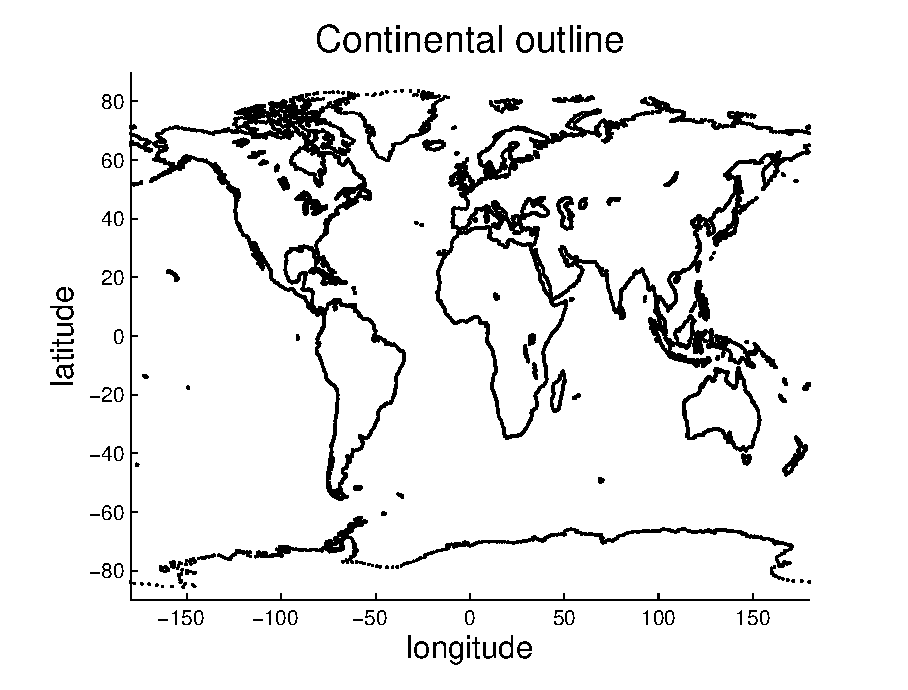
\includegraphics[width=\linewidth]{ch3-continentaloutline.eps}
\caption{Continental outline (of sorts).}
\label{fig:ch3-continentaloutline}
\end{marginfigure}

Your \textit{script} \textbf{m-file}) for this might look like:

\begin{docspecbold}
lon = load('continental\_outline\_lon.dat','-ascii');
\\lat = load('continental\_outline\_lat.dat','-ascii');
\\scatter(lon,lat);
\\axis([-180 +180 -090 +090]);
\\xlabel('longitude','fontsize',15);
\\ylabel('latitude','fontsize',15);
\\title('Continental outline','fontsize',18);
\end{docspecbold}

\noindent (but with lots of comment lines!).

By plotting dots (points), the coastal outline at higher latitudes gets increasingly pixelated. So, we might instead plot as lines between the lon-lat pairs. For this, you could simply use \texttt{plot}. 

Copy your m-file (make sure it was saved first!), rename it, and then edit it to use \texttt{plot} instread of \texttt{scatter}. You should end up with something like Figure \ref{fig:ch3-continentaloutline2}.. 
\begin{marginfigure}[0.0in]
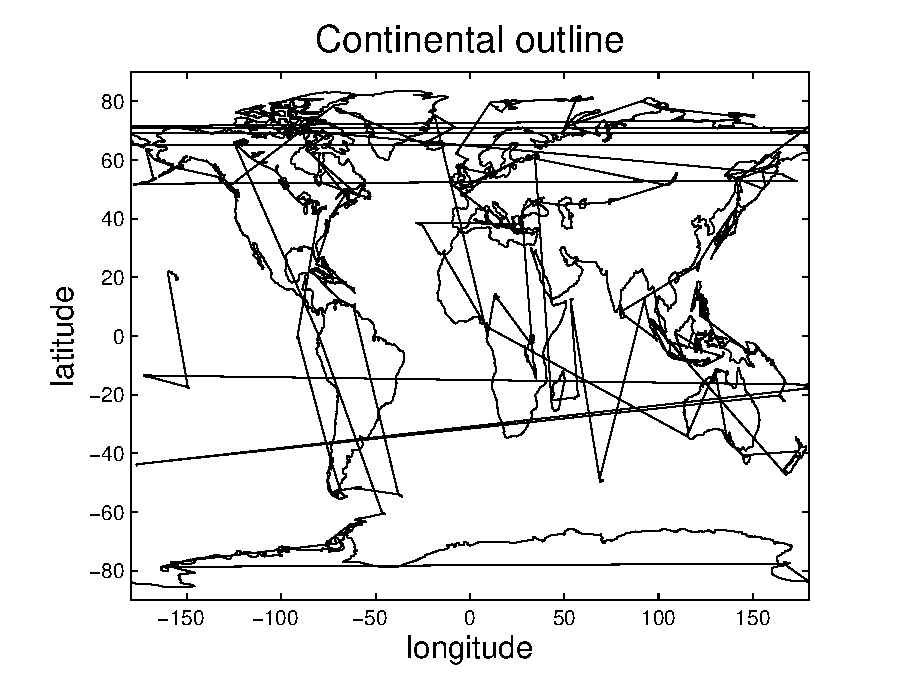
\includegraphics[width=\linewidth]{ch3-continentaloutline2.eps}
\caption{Another continental outline (of sorts).}
\label{fig:ch3-continentaloutline2}
\end{marginfigure}

Well ... interesting. If you think about it, as one continental outline is completed, the next lon-lat pair will be for the next continent or island. What \texttt{plot} does is to join up *all* the adjacent x-y (lon-lat) pairs and hence points, which is why you get the straight lines criss-crossing the map with  the start of each successive continent and island in the dataset joined to the end of the previous one.

The continental outline dataset is not actually that useless. There are  additional files that specify which block of lon-lat pairs belong to a single shape (i.e. continent or island). Load in the 2 additional files:
\begin{itemize}[noitemsep]
\setlength{\itemindent}{.2in}
\item \textsf{continental\_outline\_start.dat} (labelled '\textsf{start}')
\item \textsf{continental\_outline\_end.dat} (labelled '\textsf{end}')
\end{itemize}
i.e.:
\begin{docspecbold}
>> lstart = load('continental\_outline\_start.dat','-ascii');
\\>> lend = load('continental\_outline\_end.dat','-ascii');
\end{docspecbold}
(Note that you \uline{cannot} simply call the second variable \texttt{end}, because \textbf{MATLAB} is already using it as a special word.)

These vectors hold information regarding the start  and end row number, of each of the individual shape segments. Again, view the contents of these vectors to get an idea of what is going on. For example, you'll see that the first entry is that the first shape starts on row \texttt{1} 
(\texttt{lstart(1)}), and ends on row \texttt{100} (\texttt{lend(1)}). The 2nd shape starts on row \texttt{101} (\texttt{lstart(2)}), and ends on row \texttt{200} (\texttt{lend(2)}). etc etc

The simplest way too start dealing with all this, is to just plot the very first shape, defined by rows \texttt{1-100} of the lon and lat vectors. By now, you hopefully will be able to see that to plot rows \texttt{1-100} of  lon and lat data, you are going to do: 
\begin{docspecbold}
>> plot(lon(1:100),lat(1:100));
\end{docspecbold}

\marginnote[0.875in]{\begin{mdframed}[backgroundcolor=gray!10, roundcorner=10pt,leftmargin=1, rightmargin=1, innerleftmargin=5, innerrightmargin=5, innertopmargin=5,innerbottommargin=5, outerlinewidth=1, linecolor=gray!10]
\docenvdef{length}
\\This function could almost not be simpler -- just pass the name of a vector, and it returns its length (i.e. the number of rows, or columns, depending on the shape of the vector).
\end{mdframed}}

Well ... this is probably about as unexciting as it gets -- a small piece of the Antarctic coastline. If you do a \texttt{hold on} and plot the next block (rows \texttt{101-200}), you'll get the next chunk of coastline:
\begin{docspecbold}
>> plot(lon(101:200),lat(101:200));
\end{docspecbold}
You could keep going this -- manually adding additional sections of the global continental outline. This could get tedious ... and it turns out that there are 283 different fragments to plot, all one after another. (This number comes from asking \textbf{MATLAB} the \texttt{length} of \texttt{lstart} or \texttt{lend}, e.g. \texttt{length(lstart)}) This is, of course, why we need to get clever with a \textit{loop} and automatically go through all 283 fragments, plotting them on on top of another in the same figure.

How? First you need to write the \texttt{plot} command in a more general form -- you do not want to have to read the values out of the \texttt{lstart} and \texttt{lend} vectors manually. Hopefully, it should be apparent that you can re-write the plot statement for the first fragment, as:
\begin{docspec}
plot(lon(LINE\_START:LINE\_END),lat(LINE\_START:LINE\_END));
\end{docspec}
where for the first fragment, the values of \texttt{LINE\_START} and \texttt{LINE\_END} are given by \texttt{lstart(1)} and \texttt{lend(1)}, respectively (renaming the original vectors to shorten the variable name)\sidenote{You cannot use the obvious variable name \texttt{end} -- why not?}. Re-writing again, for the first fragment, this looks like:
\begin{docspecbold}
plot(lon(lstart(1):lend(1)),lat(lstart(1):lend(1)));
\end{docspecbold}

Try this and check you still get the single piece of the Antarctic coastline.

You should hopefully be making the mental leap to looking at \texttt{(1)} and thinking that it could be: \texttt{(n)}, where \texttt{n} is a loop counter, which could go from 1 to 283 and hence loop through all the line fragments. Yes? For instance, setting \texttt{n=1}, and plot (with \texttt{n} replacing \texttt{1} in the code fragment above) -- you should again get that very  first fragment. Try setting \texttt{n=283} and plot. Do you get the last fragment (what is it of\sidenote[][1.0 in]{An island at about 20N and -150E if you have done it correctly.})?

So ...\textbf{ create yourself a new m-file} (and copy-paste whatever you like from the previous \textit{script} tha saves you time)in terms of loading in the data. At the start -- load in the lon-lat pairs as vectors (renaming then to something more manageable if you wish) and then load in the vectors containing the start and end information. 

After that in the code -- create a \texttt{do ... end} loop. Maybe before you try and plot anything, print (\texttt{disp}) the loop count and run the program (after saving), just to check first that the loop is functioning correctly. 

Also before the loop starts, create a \textsf{Figure window}. and set \texttt{hold on}. You now have a basic shall of a program -- loading in the data, initializing a figure, and appropriate looping, but not yet actually doing anything within the loop.

In the \textit{loop} all you need is the \texttt{plot} command, but with the start and end rows being a function of \texttt{n} (or whatever you call the loop counter). Set axis dimensions and label nicely (after the loop ends).

Run it. Hopefully ... something like Figure \ref{fig:ch3-continentaloutline3} appears(?)

\begin{marginfigure}[0.0in]
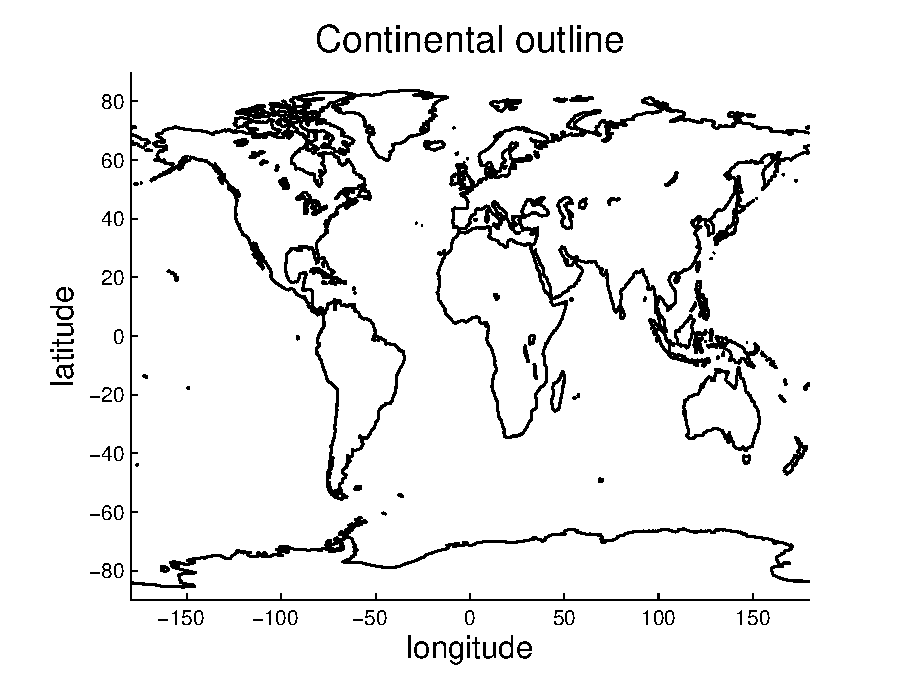
\includegraphics[width=\linewidth]{ch3-continentaloutline3.eps}
\caption{Another go at the continental outline!}
\label{fig:ch3-continentaloutline3}
\end{marginfigure}

\uline{An example code is given at the end of the text should you need any guidance as to e.g. in what order or where certain lines should go.}

%----------------------------------------------------------------------------------------
% CHAPTER 3
%----------------------------------------------------------------------------------------

\chapter{Further ... MATLAB and data visualization}
\label{ch:03}

%------------------------------------------------
%
This chapter is something of a potpourri of \textbf{MATLAB} data and visualization methodologies and techniques, generally building on the basics covered in the previous chapters.

%------------------------------------------------

\newpage

%------------------------------------------------

\section{Further data input}

Previously, you imported ASCII data into \textbf{MATLAB} using the \texttt{load} command\sidenote{Or maybe 'cheated' and used the \textbf{MATLAB} GUI ...}. You might not have realized it at the time, but the use of \texttt{load} requires that your data is in a fairly precise format. \textbf{MATLAB} says "\textit{ASCII files must contain a rectangular table of numbers, with an equal number of elements in each row. The file delimiter (the character between elements in each row) can be a blank, comma, semicolon, or tab character. The file can contain MATLAB comments (lines that begin with a percent sign, \%).}" Firstly, your data may not be in a simple format and often may contain both numerical values and string values. Secondly, your data may not even be in a text/ASCII format. For instance, you data maybe be in an \textbf{Excel} spreadsheet, or for spatial scientific data, an increasingly common format is called '\textbf{netCDF}' (Network Common Data Form). In this section, we'll go through the basics and some examples of each.

Please regard this section as a simple overview on some of the different \textbf{MATLAB} file loading/input options. At this stage, it is more important that you are aware of different data formats and the various ways of importing them into \textbf{MATLAB},  then \textit{per se} having to master all the details of using them. For many one-off data loading problems, it can be easier to use the \textbf{MATLAB} GUI and the \textsf{Import Data} wizard. 

%------------------------------------------------

\subsection{Formatted text (ASCII) input}

The general procedure that you need to follow to input formatted text data is as follows:

\marginnote[-3.0in]{\begin{mdframed}[backgroundcolor=gray!10, roundcorner=10pt,leftmargin=1, rightmargin=1, innerleftmargin=5, innerrightmargin=5, innertopmargin=5,innerbottommargin=5, outerlinewidth=1, linecolor=light-gray]
\textbf{opening and closing files}
\\\textbf{MATLAB} has a pair of commands for opening and closing files for read/write:
\begin{itemize}[noitemsep]
\setlength{\itemindent}{.2in}
\item \docenvdef{fopen} will open a file. It needs to be passed the name (and path if necessary) of the file (as a string), and will return an ID for the file (assign (save) this  to a variable -- you'll need it!).
\item \docenvdef{fclose} ... will close the file. It requires the ID of the file (i.e. the variable name you assigned the result of calling \texttt{fopen} to) passed to it as a parameter. 
\end{itemize}
\end{mdframed}}

\marginnote[-0.5in]{\begin{mdframed}[backgroundcolor=gray!10, roundcorner=10pt,leftmargin=1, rightmargin=1, innerleftmargin=5, innerrightmargin=5, innertopmargin=5,innerbottommargin=5, outerlinewidth=1, linecolor=light-gray]
\docenvdef{textscan}
\\According to (actually, paraphrased from) \textbf{MATLAB}:
\begin{docspecmargin}
C = textscan(ID,format)
\end{docspecmargin}
"\textit{ ... reads data from an open text file into a cell array, \texttt{C}. The text file is indicated by the file identifier, \texttt{ID}. Use \texttt{fopen} to open the file and obtain the \texttt{ID} value. When you finish reading from a file, close the file by calling \texttt{fclose(ID)}.}"
\\The \texttt{ID} part should be straightforward (if not -- follow through the Example).
\\The \texttt{format} bit is the complicated bit ... There is some help in a following Box and via the Example. Otherwise, there is a great deal of details and examples in \textbf{MATLAB help} -- you could look at this as a sort of menu of possibilities, and given a particular file import problem, the best thing to do is simply scan through help, looking for something that matches (or is close to) your particular data problem (and/or ask Google).
\end{mdframed}}

\begin{enumerate}[noitemsep]
\setlength{\itemindent}{.2in}

\vspace{1mm}
\item First, you need to 'open' the file -- the command (function) for this is called \docenv{fopen} (see Box). You need to assign the results of this \textit{function} to a \textit{variable} for later use.

What is going on and why this all differs so much form using \texttt{load}, where you only had to use a single command, is that you first have to open a connection to the file ... before you even read any of the contents in(!!!)\sidenote{This is very common across all(?) programming languages.}.

\vspace{1mm}
\item Secondly ... you can read the content in (finally!). The complications here include specifying the format of the data you are going to read in. You also need to tell \textbf{MATLAB} the ID of the file that you have opened (so it knows which one to read from) -- this is the value returned by the \textit{function} \texttt{fopen}. The \textit{function} you are going to use to actually read the data (having opened the file) is called \texttt{textscan}.

\vspace{1mm}
\item Once the data has been read it -- close the file using \docenv{fclose} (see Box). You are going to have to pass the ID of the  file again when you call this \textit{function} (so \textbf{MATLAB} knows which file to close).

\vspace{1mm}
\item Lastly, you are going to have to deal with the special data structure that \textbf{MATLAB} has created for you ...

\end{enumerate}

If you are interested (probably not) -- the connection made to an open file is called a file \textit{pipe}. Typically, you have have multiple open file \textit{pipes} at the same time in programs, and this is why obtaining and then specifying a unique ID for the \textit{pipe} you wish to read or write through, is critical.

\vspace{1mm}
\noindent\rule{4cm}{0.5pt}
\vspace{-2mm}

\newthought{As an initial Example} to illustrate this alternative (and more flexible) means of importing of ASCII (text) data, we are going to return to the paleo atmospheric CO\(_{2}\) proxy dataset file -- \textsf{paleo\_CO2\_data.txt}. Assuming that you have already (previously) downloaded it,  open it up in a text editor and view it -- you should see 4 neatly (ish) aligned columns of numeric values ... and 'nothing else'.

OK -- so having seen the format of the  data in the ASCII file, you are going to work through the following steps (you can do all this at the command line, or add the lines one-by-one to a \textit{script} m-file if you prefer)\sidenote{You can start off working at the command line if you wish, but ultimately, you are going to need to put everything into an \textbf{m-file}.}:

\begin{enumerate}[noitemsep]
\setlength{\itemindent}{.2in}

\item First 'open' the file -- you will be using the \textit{function}  \docenvdef{fopen}, and passing it the filename\sidenote[][-0.0in]{For convenience, you could assign the filename (+ its path) to a (string) variable and then simply pass the variable name -- remember, no \texttt{' '} needed for a variable naming containing a string (whereas \texttt{' '} is needed for the string itself).} (including the path to the file if necessary, i.e. if the \textbf{MATLAB} working directory does not also contain the file). So that you can easily refer to the file that you have opened later, assign the output of \docenv{fopen}\sidenote[][-0.0in]{The output is a simple integer index, whose value is specific to the file that you have opened.} to a variable, e.g.
\begin{docspecbold}
>> openfile\_id = fopen('paleo\_CO2\_data.txt');
\end{docspecbold}

\vspace{1mm}
\item Now ... this is where it gets a  trickier -- the \textit{function} you are going to use now is called \docenv{textscan}. Refer to \textsf{help} on \docenv{textscan}, but as a useful minimum, you need to pass 3 pieces of information:
\begin{enumerate}[noitemsep]
\setlength{\itemindent}{.2in}
\item The ID of the open file (you have assigned this to a handy variable (\texttt{openfile\_id}) already.)
\item The \textit{format} of the file (see margin note).(This is where it gets much less fun, but hang in there!) You simply list, space-separated, and between a single set of quotation marks, one format specifier per element of data.
\\In this particular Example, there are 4 items of data (per row) -- each of them is either an integer or a floating point number\sidenote{At least, none of them are clearly strings, right?}, depending on how you want to look at it. Assuming that the data is a floating point number, the \textit{format} for the input of each number item, is \texttt{\%f}.
\end{enumerate}
The result of \docenv{textscan} is then assigned to a parameter, e.g.
\begin{docspecbold}
my\_data = textscan(openfile\_id,'\%f \%f \%f \%f');
\end{docspecbold}
Here, the \texttt{'\%f \%f \%f \%f'} bit specifies that the data format consists of 4 floating point (real) numbers.

\vspace{1mm}
\item So far, so good! And you can now close the file:
\begin{docspecbold}
>> fclose(openfile\_id);
\end{docspecbold}

\marginnote[-2.0in]{\begin{mdframed}[backgroundcolor=light-gray, roundcorner=10pt,leftmargin=1, rightmargin=1, innerleftmargin=5, innerrightmargin=5, innertopmargin=5,innerbottommargin=5, outerlinewidth=1, linecolor=light-gray]
According to \textbf{MATLAB} \textsf{help}:
\\"\textit{the \texttt{format} is a string of conversion specifiers enclosed in single quotation marks. The number of specifiers determines the number of cells in the cell array C.}" Take this to mean that you need one format specifier, per column of data. The specifier will differ whether the data element is a number or character (and \textbf{MATLAB} will further enable you to create specific numerical types).
\\The format specifiers are all listed under \texttt{help textscan}. However, your Dummies Guide to \texttt{textscan} (and good for most common applications) is that the following options exist:
\texttt{
\\\%d -- (signed)integer
\\\%f -- floating point number
\\\%s -- string
}
\\\textbf{MATLAB} will automatically repeat the format for as many lines as there are of data. Alternatively you can specify precisely how many times you would like the format repeated (and hence data read in).
\end{mdframed}}

\vspace{1mm}
\item Actually, it does get darker before the light at end of the tunnel ... what \docenv{textscan} actually returns -- the data that was read in, is placed into an odd structure called a \textit{cell array}. It is not worth our while worrying about just what the heck this is, and if you view it in the \textsf{Variables} window (i.e. double click on the \texttt{cell array} name in the \textsf{Workspace} window), it does not display the simple table of 4 columns of data that maybe you were expecting. For now, we can transform this format into something that we are more familiar with using the \docenv{cell2mat} function, e.g.
\begin{docspecbold}
my\_data\_array = cell2mat(my\_data);
\end{docspecbold}
\end{enumerate}

And now ... it is done, i.e. there  exists a simple array, of 4 columns, the first being the age (Ma), the second being the CO\(_{2}\) concentration value (units of ppm), and the 3rd and 4th; minimum ad maximum error estimates in the proxy reconstructed value. :)

To help you -- \uline{a complete code for doing all this is given at the end of the book}.

\marginnote[-1.25in]{\begin{mdframed}[backgroundcolor=gray!10, roundcorner=10pt,leftmargin=1, rightmargin=1, innerleftmargin=5, innerrightmargin=5, innertopmargin=5,innerbottommargin=5, outerlinewidth=1, linecolor=light-gray]
MATLAB claims that a \docenvdef{cell array} is "\textit{A cell array is a data type with indexed data containers called cells. Each cell can contain any type of data. Cell arrays commonly contain pieces of text, combinations of text and numbers from spreadsheets or text files, or numeric arrays of different sizes.}" I am sort of prepared to believe this.
\\Basically, in object-oriented speak, a cell array is an object, or rather, an array of objects. As \textbf{MATLAB} hints -- the cells can contain *anything*. Your limitation previously is that an array had to be all floating point numbers, all integers, or all strings, and if strings, all the strings had to be the same size. For strings in particular, it is obvious that a more flexible format where a vector could contain both 'banana' and 'kiwi' is needed (try creating a 2-element vector with these 2 words and see what happens). You clearly might also want to link a number with a string (e.g. number of bananas) in the same array, rather than have to create 2 sperate arrays.
\end{mdframed}}

\vspace{1mm}
\noindent\rule{4cm}{0.5pt}
\vspace{-2mm}

\newthought{As a further example},  we are going to process a more complicated version of the paleo atmospheric CO\(_{2}\) proxy dataset. This file is called \textsf{paleo\_CO2\_data.dat} (rather than \textsf{.txt}) and is again available from the course webpage. An initial problem here is even opening up the file to view it -- if you use standard \textbf{Windows} editors such as \textbf{Notepad} it fails to format it properly when displaying its contents\sidenote{If you use a \textbf{Mac} (or \textbf{linux}) however, all text editors should display the content jus fine.}. 

The first lesson then in scientific computing then is to have access to a more powerful/flexible editor than default/built-in programs such as \textbf{Notepad}. One good (\textbf{Windows}) alternative is \textbf{Notepad++}.\sidenote{Right-mouse-button-click over the file, then select \textbf{Open with} and then click on \textbf{Notepadd++}.}

If you can open the file with something like \textbf{Notepad++} (or are in any case using a \textbf{Mac}) -- first note the format -- there are a bunch of header lines and moreover, some of the columns are not numbers (but rather strings). Even if you were to manually edit out the headers by adding \docenv{comments} (\texttt{\%})\sidenote{Recall that \textbf{MATLAB} ignore lines starting with a \texttt{\%} and this includes loading in data lines using \texttt{load}.}, you are still left with the problem of mis-matched columns. You could edit the file in \textbf{Excel} to remove the problematic columns as well ... but now this seems like a real waste of time to be editing data formats with one software package just to get it into a second! (Again, you could use the \textbf{MATLAB} GUI import functionality
... but it will be a healthy life experience for you to do it at the command line :o) )

OK -- so having gotten an idea of the format of the ASCII data file, you are going to tackle this in the same 4 steps as before:

\vspace{-2mm}
\begin{enumerate}[noitemsep]
\setlength{\itemindent}{.2in}

\vspace{1mm}
\item First 'open' the file as you did previously (using \docenv{fopen}) and assigned the ID returned by the \texttt{fopen} \textit{function} to the variable: \texttt{file\_id2}.

\vspace{1mm}
\item Call \texttt{textscan}. However, we now want to pass 3 pieces of information (compared to 2 before):
\begin{enumerate}[noitemsep]
\setlength{\itemindent}{.2in}
\item The ID of the open file.
\item The \textit{format} of the data.
\item And now -- a parameter, together with an (integer) value, to specify how many rows of the file are to be assumed to be  header information and hence skipped.
\end{enumerate}

(Again -- the result of \docenv{textscan} is then assigned to a variable which will represent a \textit{cell array}.)

Lets do the easy bit first -- to tell \textbf{MATLAB} to skip \textit{n} lines of a file. For this -- add the parameter \texttt{'HeaderLines'} to the list of parameters passed to \texttt{textscan}, and then simply tell it how many lines to skip. In this example:
\begin{docspec}
my\_data = textscan( ...
\\ \ \ \ \ \ file\_id2, ... ,'HeaderLines',3);
\end{docspec}
will tell \textbf{MATLAB} to skip the first 3 lines of the file.

OK -- now to dive back into the \textbf{MATLAB} syntax mire ... Let us just load in just the first 2 columns of data, and assume that they are both integers (and also skipping the first 3 lines of the file as per above). We might guess that we could simply write:
\begin{docspec}
my\_data = textscan( ...
\\ \ \ \ \ \ file\_id2,'\%d \%d','HeaderLines',3);
\end{docspec}

Try it (including closing the file, and a call to \texttt{cell2mat}, as before). What has happened?

It seems that \textbf{MATLAB} translates your format (\texttt{'\%d,\%d'}) into: 'read in a pair of integers, and keep automatically repeating this, until something else is encountered'. That something else, is sequence of characters at the end of the first data line (line \#4, because we skipped the first 3), that makes \textbf{MATLAB} think that it has finished (or rather, that it cannot reading in 2 pairs of integers any longer). This leaves you with 2 pairs of integers -- i.e. a 2\(\times\)2 matrix (as you'll see if you look at \texttt{my\_data\_array}).

Here is a solution -- we could omit all the information following the first 2 elements (something for \textbf{Google} to help with).\sidenote{This turns out to be specifying \texttt{'\%*[\(^{\wedge}\)$\backslash$n]'}, which in effects sort of says:\\'skip everything (all the fields) (\texttt{\%*}) up until the end of the line is found (\texttt{[\(^{\wedge}\)$\backslash$n]}).}: \begin{docspec}
my\_data = textscan( ...
\\ \ \ \ \ \ file\_id2,'\%d \%d \%*[\(^{\wedge}\)$\backslash$n]','Headerlines',3)
\end{docspec}
The weird bit here translates to ... \texttt{\%*} == ignore field ... until the line end == \texttt{[\(^{\wedge}\)$\backslash$n]}, and then read repeat for the next line.

(You are not expected to know or remember this nor be tested on it ... just park all this at the back of your mind and that there are flexible ways of dealing with data input, including not necessarily reading everything in!)

\vspace{1mm}
\item Now you can close the file:
\begin{docspec}
fclose(file\_id2);
\end{docspec}

\vspace{1mm}
\item ... and convert the results to something  human-readable:
\begin{docspec}
my\_data\_array = cell2mat(my\_data);
\end{docspec}

\end{enumerate}

This should do it -- a simple array, of 2 columns, the first being the age (Ma) and the second the CO\(_{2}\) concentration value (units of ppm). :)

\marginnote[-8.5in]{\begin{mdframed}[backgroundcolor=gray!10, roundcorner=10pt,leftmargin=1, rightmargin=1, innerleftmargin=5, innerrightmargin=5, innertopmargin=5,innerbottommargin=5, outerlinewidth=1, linecolor=light-gray]
\docenvdef{cell2mat}
\\Having created this weird format (\docenv{cell array}), now MATLAB has to give you a way of converting the data inside into something more usable. The function is \docenv{cell2mat}, which for a cell array C:
\begin{docspecmargin}
A = cell2mat(C);
\end{docspecmargin}
will return the corresponding ('normal') array A.
\\Now this is only true if all the data in \texttt{C} is of the same tpye (e.g. all floating point numbers). If the data types are mixed or you only wish for a sub-set of the data to be extracted and converted, simply index the required part of the cell array (Examples on this later).
\end{mdframed}}

The complete code (minus all the lovely comments!) looks like:
\begin{docspecbold}
file\_id2 = fopen('paleo\_CO2\_data.dat');
\\my\_data = textscan( ...
\\ \ \ \ \ \ file\_id2,'\%d \%d \%*[\(^{\wedge}\)$\backslash$n]','Headerlines',3);
\\fclose(file\_id2);
\\my\_data\_array = cell2mat(my\_data);
\end{docspecbold}
(remembering that the \texttt{...} just indicates a break in what is otherwise a continuous single line).

Put this into a new \textit{m-file}, comment it, so that you know what all the bits are doing (and what the overall program itself  does), and try it out. NOTE: if you copy-paste from the textbook PDF ... be careful not only to replace the PDF inverted comma character with a 'normal' (\textbf{MATLAB}-friendly one), but the \(^{\wedge}\) symbol can also come out incorrectly
\sidenote{The symptom being that only the first line of data is read in.} ...
 
(There must be some sort of important life lesson hidden here in all this. Perhaps about only working with well-behaved data files, or using the GUI import functionality?)

%------------------------------------------------

\subsection{Importing ... Excel spreadsheets}

If your data is contained in an \textbf{Excel} spreadsheet, which is a common occurrence, and you want it in \textbf{MATLAB}, your options are:

\vspace{-2mm}
\begin{enumerate}[noitemsep]
\setlength{\itemindent}{.2in}
\vspace{1mm}
\item Select some, or all, of the columns and rows in a specific worksheet, and either copy-paste this into a text file (but taking care that the worksheet column widths are formatted such that they are wider than the widest data element), or save in an ASCII format, with comma or tab delineations between columns. In either case, then load in the data using \texttt{load}, or if consisting of mixed numbers/text, go through the Hell that is \texttt{textscan} ....
\vspace{1mm}
\item Use \textbf{MATLAB} \textit{function} \docenv{xlsread}.
\end{enumerate}

So ... option \#2 looks ... is looking the easiest ... :)

\marginnote[-1.0in]{\begin{mdframed}[backgroundcolor=gray!10, roundcorner=10pt,leftmargin=1, rightmargin=1, innerleftmargin=5, innerrightmargin=5, innertopmargin=5,innerbottommargin=5, outerlinewidth=1, linecolor=light-gray]
\docenvdef{xlsread}
\\There are various uses (i.e. alternative allowed syntax) for \docenv{xlsread} for an \textbf{Excel} file with name \texttt{filename}. The 2 relevant and more useful ones look to be:
\begin{enumerate}[noitemsep]
\setlength{\itemindent}{.2in}
\item \texttt{num = xlsread(filename)}
which will return the *numeric* data in the Excel file \texttt{filename} in the form of a matrix, \texttt{num}. Note that non-numeric (e.g. string) headers and/or columns, are ignored. Also note that \texttt{num} is a 'normal' numeric array and does not require any conversion.
\item \texttt{[num,txt,raw] = ... 
\\ \ \ \ \ xlsread(filename)}
will additionally return text data in a \textit{cell array} \texttt{txt}, and *everything* in a cell array \texttt{raw}.
\end{enumerate}
You can also specify a particular worksheet out of an Excel file to load in:
\begin{docspecmargin}
num = ...
\ \ \ \ xlsread(filename,sheet)
\end{docspecmargin}
(and there are further refinements and options listed under \textbf{help}).
\end{mdframed}}

\vspace{1mm}
\noindent\rule{4cm}{0.5pt}
\vspace{-2mm}

\newthought{Returning to the paleo proxy CO\(_{2}\) data ...} but this time, as an \textbf{Excel} sheet. The data file you need is: \textsf{paleo\_CO2\_data.xlsx}
\\\noindent (You may as well go load this into \textbf{Excel} just to take a look at the format and so subsequently, you'll know if you have imported it faithfully or not.)

From the help box on \texttt{xlsread}, it should be pretty apparent what you do. And in fact, I am going to leave you to work it out -- try and import the age and CO\(_{2}\) data from \textsf{paleo\_CO2\_data.xlsx}.

Note that the simple usage of the \texttt{xlsread} \textit{function} gives you an \textit{array} containing just the numeric data. If you were to type:
\begin{docspecbold}
>> [num,txt,raw]=xlsread('paleo\_CO2\_data.xlsx');
\end{docspecbold}
then you still get the numeric data returned in the array \texttt{num}, but you also get 2 \textit{cell arrays}\footnote{
If you need to index a cell array, you do so pretty well much like a normal array, except it has an alternative syntax. For a normal, numeric array \texttt{A}, you might write:
\begin{docspecmargin}
>> A(4,3)
\end{docspecmargin}
to reference the value in the 4th row, 3rd column. For a \textit{cell array }\texttt{C}, to index the cell in the 4th row, 3rd column, you'd also write:
\begin{docspecmargin}
>> C(4,3)
\end{docspecmargin}
but you'd get a cell returned, not the value in the cell. If you want the value in the cell located at \texttt{(4,3)}, you'd put the index in curly brackets:
\begin{docspecmargin}
>> C\{4,3\}
\end{docspecmargin}
and you'd get a value of \texttt{3000} returned in this example.} -- \texttt{txt} and \texttt{raw}.  The \textit{cell array} \texttt{txt} contains just the text data, and \texttt{raw}, 'everything'. View these in the \textsf{Variable window} (by double-clicking on the variable names in the \textbf{MATLAB} \textsf{Workspace window}). NOTE that \textbf{MATLAB} takes some time to open and process \textbf{Excel} format files and the command will not complete as quickly as e.g. \texttt{load}.

If you happen to have an \textbf{Excel} file with data (of any sort) in it (e.g. from another class), practice loading in its contents into \textbf{MATLAB}. Note that if the \textbf{Excel} file contains cells with text in and you want the text data, then you'll need to use the more advanced format of \texttt{xlsread} (see Box or \texttt{help}). Also try loading into only a single sheet of an \textbf{Excel} file (assuming that the file has multiple sheets). 

%------------------------------------------------

\subsection{Importing ... netCDF format data}

Much of spatial, and particularly model-generated, scientific output, is in the form of \textit{netCDF} files. This is a format designed as a common standard to facilitate sharing and transfer of spatial data, but in a way that enables e.g. a 'complete' description of dimensions and various types of meta-data to be incorporated along with the data. The format is platform independent and a variety of graphical viewers exist for viewing and interrogating the data. Most programming languages support the reading and writing of \textit{netCDF} format data. \textbf{MATLAB} is no exception here.

\textbf{MATLAB} actually has a quick and simple (\uline{concentrate on this first one}!), and ... a complicated long-winded formal way (simply note the existence of this one!) of accessing data in a \textit{netCDF} file:

\marginnote[-0.625in]{\begin{mdframed}[backgroundcolor=gray!10, roundcorner=10pt,leftmargin=1, rightmargin=1, innerleftmargin=5, innerrightmargin=5, innertopmargin=5,innerbottommargin=5, outerlinewidth=1, linecolor=light-gray]
\docenvdef{ncread}
\\In its simplest incarnation:
\begin{docspecmargin}
data = ... ncread(filename,varname)
\end{docspecmargin}
where \texttt{filename} is the name of a \textit{netCDF} file, and \texttt{varname} is the name of the data variable in the \textit{netCDF} file.
\\e.g. if there was a variable called \texttt{rain} in the file \texttt{climate.nc},
\begin{docspecmargin}
data = ... ncread('climate.nc','rain')
\end{docspecmargin}
would read the values in the \textit{netCDF} file variable \texttt{rain} and assign to the variable \texttt{data}.
\\\textbf{MATLAB} provides a couple of further tricks, allowing you to read sections of the full \textit{netCDF} variable data array, or sample the data array -- see \textbf{help}.
\end{mdframed}}

\begin{enumerate}

\item Using \docenv{ncread}, which reads data directly from the file.

\noindent \docenv{ncread} is by far the simplest way, although it lacks in flexibility and deviates from standard practices used across other programming languages.

\item Via a series of function calls to the netCDF library.

\noindent In the formal and more long-winded approach, you open the file and receive an ID for that file. The file can then be written to or read (including just interrogating its properties rather than necessarily extracting spatial data) using this ID. And of course, closed (using the same ID). The \textit{netCDF} standard is also little odd in how reading/writing is implemented and everything has to be done by determining the ID of a particular data variable or property of the file. 
The general approach is as follows:

\begin{enumerate}[noitemsep]
\setlength{\itemindent}{.2in}
\item Open the netCDF file by
\begin{docspec}
\textcolor{blue}{ncid} = netcdf.open(filename,'nowrite');
\end{docspec}
where \texttt{filename} is the name of the \textit{netCDF} file (which generally will end in \texttt{.nc}). \texttt{'nowrite'} simply tells \textbf{MATLAB} that this file is being open as read-only (this is the 'safe' option and prevents accidental deletion of over-writing of data).
\item This is the weird bit, as we cannot ask for the data we want automatically :o) Instead, given that we know\sidenote{There are ways of listing the variables if not.} the name of the variable we want to access, we ask for its ID\ ...
\begin{docspec}
\textcolor[rgb]{0,0.501961,0.25098}{varid}  = netcdf.inqVarID(\textcolor{blue}{ncid},NAME);
\end{docspec}
where NAME is the name of the variable (as a string), allowing us to then request the data:
\begin{docspec}
data  = netcdf.getVar(\textcolor{blue}{ncid},\textcolor[rgb]{0,0.501961,0.25098}{varid});
\end{docspec}
that says -- assign the data represented by the variable \texttt{\textcolor[rgb]{0,0.501961,0.25098}{varid}}, in the \textit{netCDF} file with ID \texttt{\textcolor{blue}{ncid}}, to the variable \texttt{data}.
\\So actually, not totally weird -- you request the ID of the variable, then use that to get access to the data itself. The names of the \textbf{MATLAB} commands vaguely make sense in this respect -- \texttt{inqVarID} for inquiring about the ID of a variable, and \texttt{getVar} for getting the variable (data) itself\sidenote{It is beyond the scope of this course to worry about why in the case of netCDF, the function are all \texttt{netcdf.} something. Just to say, it involves objects and methods and is a common notation in object orientated languages (that nominally, \textbf{MATLAB} isn't).}.
\item Finally -- close the file, by passing the ID variable into the function \texttt{netcdf.close}, i.e.
\begin{docspec}
netcdf.close(\textcolor{blue}{ncid});
\end{docspec}
\end{enumerate}

Note that you need to pass the ID of the \textit{netCDF} file for each and every command (after \texttt{netcdf.open}) so that \textbf{MATLAB} knows which \textit{netCDF} object you are referring to (you are allowed to have multiple \textit{netCDF} files open simultaneously).

\end{enumerate}

\vspace{-1mm}
\noindent\rule{4cm}{0.5pt}
\vspace{-2mm}

\newthought{For a \textit{netCDF} Example}, we'll take the output of a low resolution climate model. To start off, download the 'model netCDF file -- 2D' \textit{netCDF} file -- \textsf{fields\_sedgem\_2d.nc}. The data here is relatively simple -- a 2D distribution of bottom-water and surface sediment properties, saved at a single point in time. In other words, there are only 2 (spatial) dimensions to the data\sidenote[][-1.0in]{Adding time would make it 3 dimensions (2 spatial + 1 of time). Adding height or depth in the ocean would also make it 3 (3 spatial). 3 spatial + time would make for a 4-dimensional dataset ...}.

OK -- we'll start by opening the file. The ID\ of the variable we want to extract and plot  is called \textsf{'grid\_topo'}. To load/extract the 2D field and assign it to a variable \texttt{data}:
\begin{docspecbold}
>> data2d = ncread('fields\_biogem\_2d.nc','grid\_topo');
\end{docspecbold}

You should now have an array called \texttt{data}. It should be 36\(\times\)36 in size. \textbf{Plot it}\sidenote[][-1.5in]{Your choice of 2D plotting function that you have already come across, e.g. \texttt{pcolor} or \texttt{image}, although not all work as well on this particular dataset (e.g. the auto scaling in \texttt{image} causes issues).}. Can you deduce what it might be of? Is it in the correct orientation? (If not -- correct it, by rotating the array, and/or flipping the rows or column.)

(There are more appropriate ways of plotting this, which we will encounter later.)\sidenote[][-1.25in]{Missing here are the x and y axis values, which you should have correctly deduced are longitude and latitude, respectively, with latitude presumably going from -90 to 90N, and longitude ... well, maybe it is not completely obvious exactly what the value of longitude is at the original.

A great strength of \textit{netCDF} its the ability of this file format to also contain the grid (axis) details that the data is on. There are ways of finding out the names of the axis variables (dimensions), but for now, I'll give you them:
\begin{itemize}[noitemsep]
\setlength{\itemindent}{.2in}
\item \texttt{'lat'} -- is the latitude axis. (Technically, the axis values are the mid-points of the grid cells.)
\item \texttt{'lon'} -- is the longitude axis.
\end{itemize}

The axes are held in the \textit{netCDF} file as vectors and we can retrieve this (1D) data in a similar way to the 2D data:
\begin{docspecmargin}
varid  = netcdf.inqVarID(ncid,'lat');
\\lat \ \ = netcdf.getVar(ncid,varid);
\\varid  = netcdf.inqVarID(ncid,'lon');
\\lon \ \ = netcdf.getVar(ncid,varid);
\end{docspecmargin}
in which we obtain the ID of the axis variable \texttt{'lat'}, then retrieve the axis data and assign it to a vector \texttt{lat} (and then likewise for longitude). Do this, and confirm that you get plausible vectors representing positions along a longitude and latitude axis.

The final task would then be to take the 2 axis vectors, and create a pair of matrices -- one containing longitude values associated with the 2D data points, and one containing latitude values  associated with the 2D data points. For this, you would need to use the function \texttt{meshgrid}. (We'll re-visit this example once you have seen \texttt{meshgrid} in action.)}

The variable names of other data-sets that you might load (in place of passing \texttt{'grid\_topo'})  and experiment with in terms of plotting function, color scale, and any other refinements that help visualise the data, include:

\begin{itemize}[noitemsep]
\setlength{\itemindent}{.2in}
\item \textsf{ocn\_sal} -- deep ocean salinity (units of per mil).
\item \textsf{ocn\_O2} -- concentration of oxygen in bottom waters (units of mol kg\(^{-1}\)).
\item \textsf{sed\_CaCO3} -- weight \% of calcium carbonate in surface sediments.
\end{itemize}

\vspace{-1mm}
\noindent\rule{4cm}{0.5pt}
\vspace{-2mm}

\newthought{[\textbf{\textcolor{red}{OPTIONAL}}] In a related \textit{netCDF} Example}, we'll extend the problem to 3D -- 2 spatial dimensions (longitude and latitude) and one of time. The file you will need to download to experience these wonders, is called \textsf{fields\_biogem\_2d.nc}

To load the variable \textsf{'atm\_temp'}:
\begin{docspecbold}
>> data3d = ncread('fields\_biogem\_2d.nc','atm\_temp');
\end{docspecbold}

How many dimensions does this array have (e.g. use \texttt{size}, or ensure that the \textsf{Size} column in the\textsf{ Workspace window} is selected)? What are the lengths along each dimension? Can you deduce which of the dimensions, time might be?

\textbf{Plot a lon-lat slice.} Note that you need to select all longitudes and all latitudes in the array, but only one time index.

\textbf{Finally -- to test your understanding to date, create an animation of how the surface air temperature in the model evolves over time.}\sidenote[][-0.0in]{You have everything you need -- the \textit{vector} of years, and from this you can determine how many different time points (and 2D data slices) there are, and hence the number of iterations of a \textit{loop}.}

%------------------------------------------------

\newpage

%------------------------------------------------

\section{Further (spatial / (x,y,z)) plotting}

As you have seen earlier -- the simplest possible way of taking a matrix of data values and plotting them spatially, as a function of (\textit{x,y}) location, is the function \docenv{image}. In effect, this is treating your data as if it were an image (or photograph) -- the data values being the 'color' of each pixel and the location in the matrix defining where in the image (row, column) the pixel is. The problem with this is that information regrading what is on the \textit{x} and \textit{y} axes is lost, be this distance, lat/lon, or some set of observed/experimental variables, or whatever. Instead, the points are evenly spaced on both axes. Moreover, the raw values are plotted and there is no possibility of interpolation/contouring or smoothing. One could regard scatter plotting as an improvement over this and a sort of \textit{x,y,z} plotting, in as much as a 3rd dimension (\textit{z} data value) can be represented through color and/or symbol shape and at time this can be quite effective. However, again, no interpolation/contouring or smoothing is possible with \texttt{scatter}. 

%------------------------------------------------

\subsection{Contour plotting}

For plotting true (\textit{x},\textit{y},\textit{z})/'3D' plots (i.e. data values in 2 spatial dimension), \textbf{MATLAB} provides a wide variety of more formal ways of plotting data spatially, including even the possibility of adding a 4th dimension representing the data value (\textit{x,y,z,zz}) (see Box).

\marginnote[-4.375in]{\begin{mdframed}[backgroundcolor=light-gray, roundcorner=10pt,leftmargin=1, rightmargin=1, innerleftmargin=5, innerrightmargin=5, innertopmargin=5,innerbottommargin=5, outerlinewidth=1, linecolor=light-gray]
\textbf{x,y,z PLOTTING}
\\\textbf{MATLAB} calls plots of a (\textit{z}) value as a function of both \textit{x} and \textit{y}, '3D'. Strictly, one could look at some of these functions as 2D, as scatter can plot a 3rd data (\textit{z}) value as different colors/shapes/sizes as a function of both \textit{x} and \textit{y} ... Anyway, the most commonly used/useful and fortunately simple, functions which create a 2D (\textit{x}, \textit{y}) plot but with contours in the value of (\textit{z}), are:
\begin{enumerate}[noitemsep]
\item \docenvdef{contour} -- Plots a figure with the data contoured, with a range and increment between contours that is fully specifiable, color-coded or not, and labelled or not. Options are also provided for specifying how the contouring is done (and the data interpolated).
\item \docenvdef{contourf} -- Similar to \docenv{contour}, except in between the (now simple black, by default) contours, a fill color is plotted and scaled to the data value.
\end{enumerate}
For a genuine 3D plot, with surface height determined by the data in the 3rd dimension of the array, colors and/or contours in the data in the 4th array dimension, suitable functions include:
\\\noindent \texttt{surf}, \texttt{surfc}, \texttt{mesh}
\\\noindent(but are not considered further here).
\end{mdframed}}

For a feel of what you should be able to learn to achieve using \textbf{MATLAB} -- go to the following \href{http://iridl.ldeo.columbia.edu/SOURCES/.LEVITUS94/.MONTHLY/.temp/#views}{webpage}. In this data repository you can do things like re-plot with different longitude, latitude, and temperature ranges. Overlay the coastlines, and other useful things like that. You can also click through the different months of the year to get a feel for how the surface temperatures on Earth change with the seasons. (However, the graphic produced from this particular website is not particularly great, and you will learn to do at least as good as this!)

%------------------------------------------------

\vspace{1mm}
\noindent\rule{4cm}{0.5pt}
\vspace{-2mm}

%------------------------------------------------

\newthought{As an example}, load in the '\textit{global Earth surface topography}' data file (\textsf{etopo1deg.dat}) from the course webpage. This is the height of the  (solid) surface of the Earth relative to mean sealevel in meters, with the continents having a positive value and the ocean floor, negative. The data is conveniently on a 1\degree\ (longitude and latitude) grid. You could view the resulting elements of the 2D array in the Variable window if you like ... but at 360\(\times\)180
in size, there may not be much of use you can glean by visually inspecting the matrix\sidenote[][-2.0in]{More useful then are the summary details in the \textsf{Workspace window}, such as the apparent absence of \textit{NaNs} and that the \textsf{Min} and \textsf{Max} Earth surface heights seem plausible.}.

\begin{marginfigure}[-1.25in]
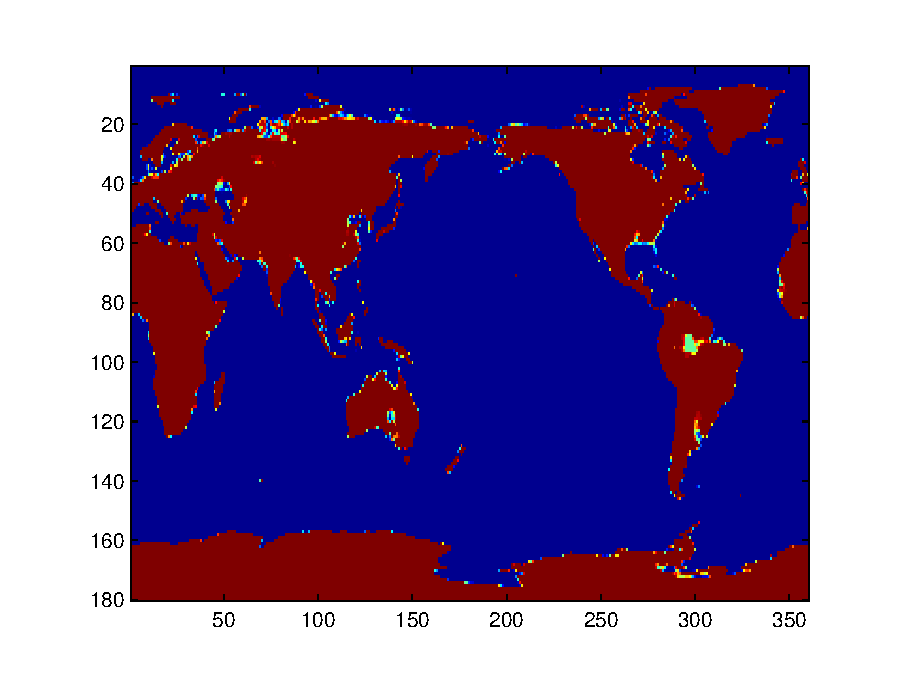
\includegraphics[width=\linewidth]{ch3-etopo.eps}
\caption{Very basic imaging (\texttt{image}) of an array (2D) of data -- here, global bathymetry.}
\label{fig:ch3-etopo}
\end{marginfigure}

After loading the data file into the \textbf{MATLAB} workspace, try throwing the array into the \texttt{image} function (which you saw previously) see what happens, e.g.
\begin{docspecbold}
>> image(etopo1deg);
\end{docspecbold}
(hopefully something like Figure \ref{fig:ch3-etopo}, but perhaps with a different default color scale). 

\begin{marginfigure}[-0.375in]
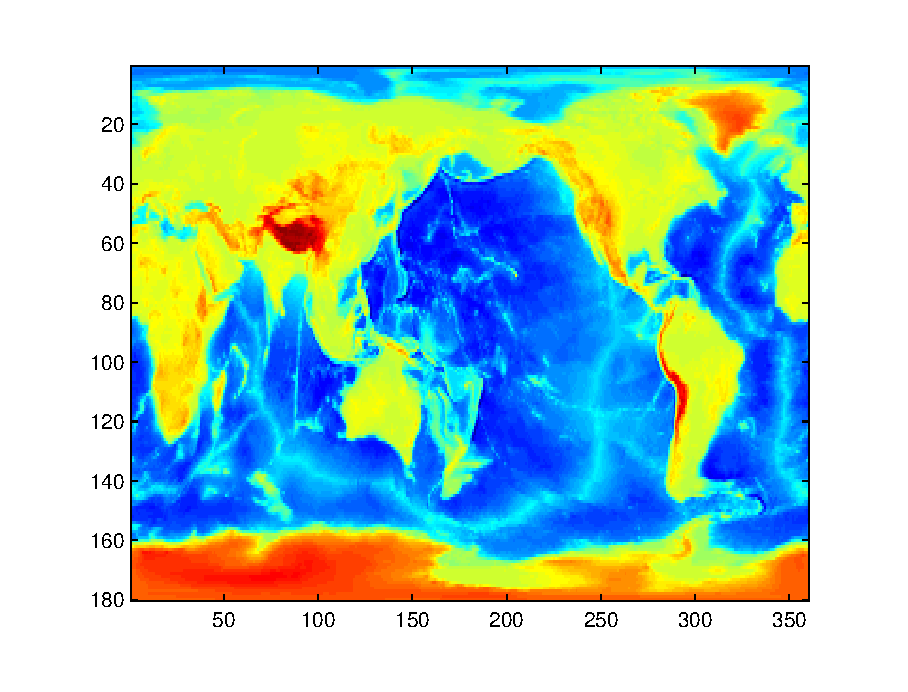
\includegraphics[width=\linewidth]{ch3-etopo2.eps}
\caption{Slightly improved very basic imaging (\texttt{imagesc}) of bathymetry data.}
\label{fig:ch3-etopo2}
\end{marginfigure}

If it had happened to come out displayed upsidedown\sidenote[][-0.0in]{It doesn't in this particular case.}, then you'd need to first (before plotting using imagesc) flip the matrix upsidedown using the command:
\begin{docspec}
etopo1deg=flipud(etopo1deg);
\end{docspec}
(and then re-plot using \texttt{image}), and if the Earth instead appeared on its side you will need to swap the rows and columns (\textit{x} for \textit{y} axis):
\begin{docspec}
etopo1deg=etopo1deg';
\end{docspec}
using the \docenv{transpose} function. It is not unusual for a first plotting attempt of spatial data to be incorrectly orientated and a little trial-and-error to get it straight is perfectly acceptable!

This is not exactly the prettiest of images. You can distinguish ocean (blue) from land (mostly brown, but other color pixels in places). Fortunately, \textbf{MALTAB} provides a variant of this plotting function, \docenvdef{imagesc} (see Box and/or \textbf{MATLAB} \textsf{help}), that calculates the color scale to exactly span the min/max values in the data. Try this alternative plotting function (and  something like Figure \ref{fig:ch3-etopo2}), e.g.
\begin{docspecbold}
>> imagesc(etopo1deg);
\end{docspecbold}

\marginnote[-3.0in]{\begin{mdframed}[backgroundcolor=gray!10, roundcorner=10pt,leftmargin=1, rightmargin=1, innerleftmargin=5, innerrightmargin=5, innertopmargin=5,innerbottommargin=5, outerlinewidth=1, linecolor=light-gray]
\docenvdef{imagesc}
\\For a data array (matrix) \texttt{A},
\begin{docspecmargin}
imagesc(A)
\end{docspecmargin}
displays the data array as if a bitmap, but unlike \texttt{image} (see earlier), \textit{"uses the full range of colors in the colormap}".
\\To set the limits of the color scale, e.g. from (\textit{z}) value of 0.0 to 10.0, you can pass the limits as a vector:
\begin{docspecmargin}
imagesc(A,[0.0 10.0])
\end{docspecmargin}
(and very similar to setting the x- or y-axis scales).
\end{mdframed}}

The function \texttt{imagesc} also enables the range of data values the color range corresponds to, to be set. Refer to \texttt{help} on this function and see if you can plot just the above-sealevel, i.e. land surface heights, spanning zero (sealevel) to the maximum height.

HINT: You can use the function \texttt{max} to determine the maximum value in a vector, and for the entire array:
\begin{docspec}
etopo1deg\_mxa=max(max(etopo1deg));
\end{docspec}
as we did for sum in the first chapter, or more elegantly:
\begin{docspec}
etopo1deg\_max=max(etopo1deg,[],'all');
\end{docspec}
(refer to \textbf{MATLAB} \texttt{help} for the syntax and why the \texttt{[]} is needed), and hence finallly to:
\begin{docspecbold}
>> imagesc(etopo1deg,[0.0 etopo1deg\_max]);
\end{docspecbold}

\marginnote[-3.5in]{\begin{mdframed}[backgroundcolor=gray!10, roundcorner=10pt,leftmargin=1, rightmargin=1, innerleftmargin=5, innerrightmargin=5, innertopmargin=5,innerbottommargin=5, outerlinewidth=1, linecolor=light-gray]
\docenvdef{colormap}
\\ \textbf{MATLAB} has a number of 'colormaps' built in -- color scale that determine the colors that correspond to the data. The command to change the \textit{colormap} from the default is:
\begin{docspecmargin}
>> colormap NAME
\end{docspecmargin}
where \texttt{NAME} is the name of the \textit{colormap}. You can find a list of possible \textit{colormaps} in \textbf{help} on \texttt{colormap} (in a table towards the bottom). But a brief summary is:
\begin{itemize}[noitemsep]
\setlength{\itemindent}{.2in}
\item \texttt{parula} -- the current \textbf{MATLAB} default -- chosen to provide a wide range of color and color intensity.
\item \texttt{jet} -- the old \textbf{MATLAB} default, but one which uses red and green in the same color, which should be avoided (why?).
\item \texttt{hot}, \texttt{cool} -- relatively simple color transitions but useful -- hot is something like you'll see in publication figures. 
\item \texttt{pink} -- another simple and at times useful transition and from dark (almost black) to white.
\end{itemize}
To return to the default \textit{colormap}:
\begin{docspecmargin}
>> colormap default
\end{docspecmargin}
\end{mdframed}}

Which sort of in a round-about sort of way also brings us to how to set the color scale, which can be changed using the \docenv{colormap} command (see Box).

\newpage

At the command line, try out setting a different \textit{colormap}, e.g.
\begin{docspecbold}
>> colormap 'pink'
\end{docspecbold}
and re-then re-plot the global topography data. Try out various different color maps/scales (\texttt{\textgreater\textgreater\ help GRAPH3D} will give a list of \textbf{MATLAB} colormaps). What color and (min,max) scales work well and what do not? Which scales help pick out details of e.g. ocean floor depth variation and which help pick out simple land-sea contrasts. Think about what one might want to highlight about global topography and what color scale might be best for this purpose?

%------------------------------------------------

\vspace{1mm}
\noindent\rule{4cm}{0.5pt}
\vspace{-2mm}

%------------------------------------------------

\newthought{Sticking with global Earth surface topography}, how else can we display the spatial data? For instance we might want to interpolate it, contour it, or simple get the longitude and latitude exes correct. Note that only by luck, because this particular dataset is 1 degree by 1 degree, the default axis scale in \textbf{MATLAB} when using image is approximately correct, although note that 'latitude' has been ordered in reverse and it goes from 1 to 180 rather than -90 to 90 ... We'll explicitly address this shortly.

To start with, you can simply use the \texttt{contour} function (see Box), passing only the matrix (of global topography values). Try this, e.g.
\begin{docspecbold}
>> contour(etopo1deg);
\end{docspecbold}

Now you might want to think about flipping the matrix up-down, and/or left-right, as your plot should have come out looking like Figure \ref{fig:ch5-contour1} (depending on your chosen colormap) and may need adjusting.

\begin{marginfigure}[0.0in]
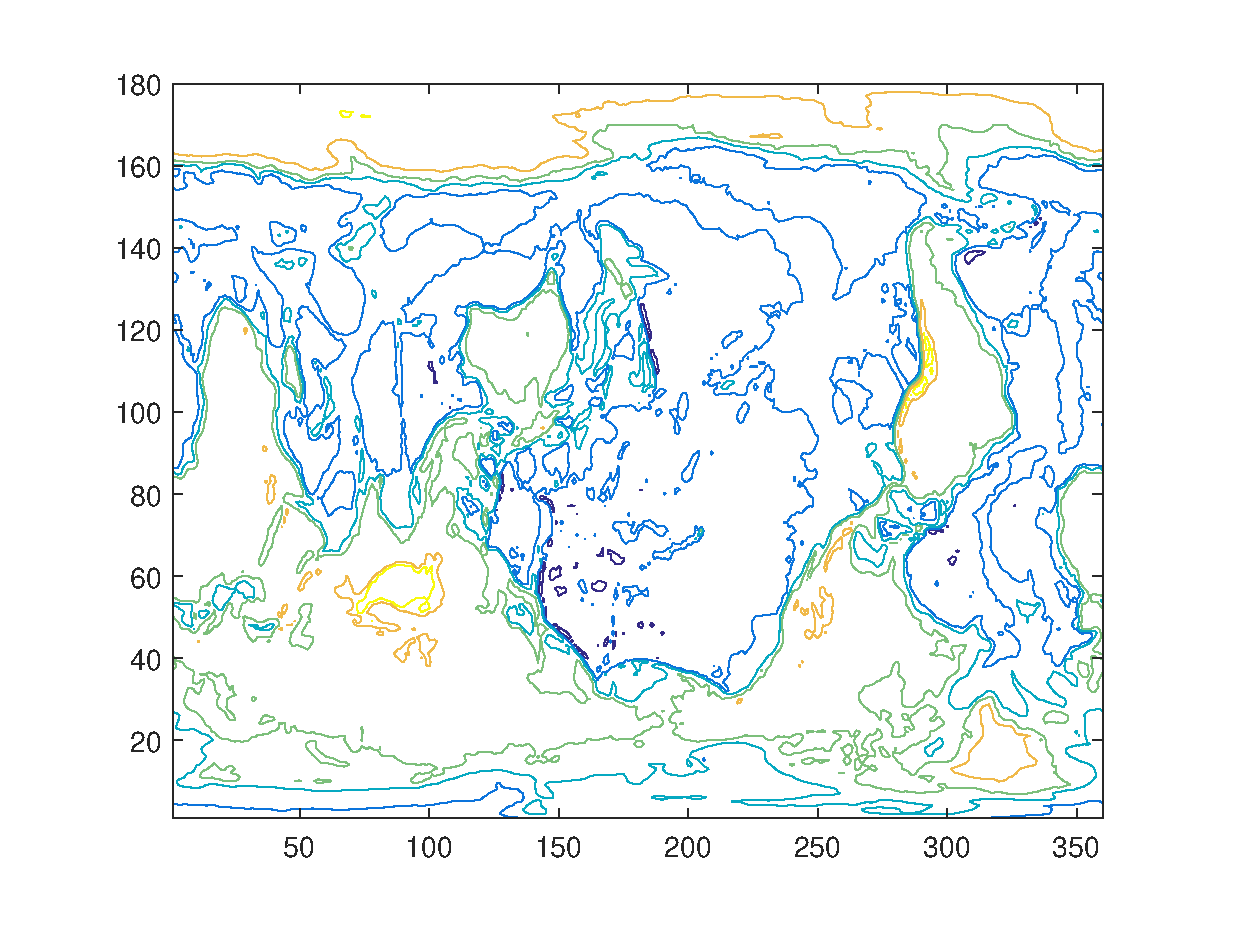
\includegraphics[width=\linewidth]{ch5-contour1.eps}
\caption{Example result of basic usage of the \texttt{contour} function.}
\label{fig:ch5-contour1}
\end{marginfigure}

Once you have fixed the orientation of the topography map, you might play about with the color scale (\texttt{colormap}) as before. You might also try the companion to \texttt{contour}, called \texttt{contourf} which gives you something like Figure \ref{fig:ch5-contour2}, e.g.
\begin{docspecbold}
>> contourf(etopo1deg);
\end{docspecbold}

\begin{marginfigure}[0.0in]
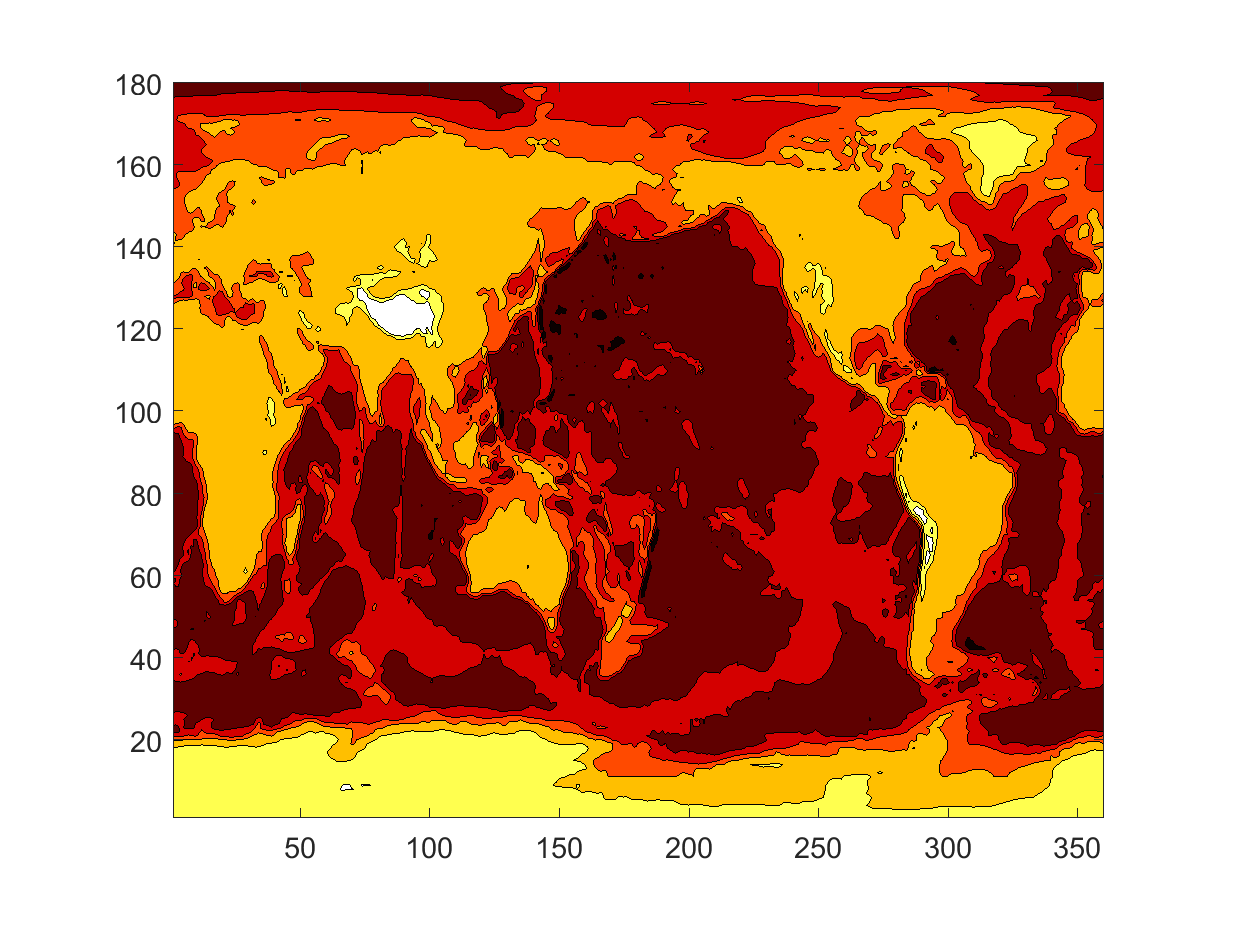
\includegraphics[width=\linewidth]{ch5-contour2.eps}
\caption{Example usage of \texttt{contourf}, with the \texttt{hot} \textit{colormap} (giving dark/brown colors as deep ocean, and light/white as high altitude).}
\label{fig:ch5-contour2}
\end{marginfigure}

OK, so a next refinement in plotting esp. maps and contour plots, is firstly, to specify the range of the color scale, as we may not want the min-to-max range chosen by default by \textbf{MATLAB}, and then, to control the number of contours (e.g. in the topography example, they are pretty far apart and it is difficult to make out much detail). Both of these factors can be addressed simultaneously, by giving \textbf{MATLAB} a vector containing the value at which you want the contours drawn\sidenote{By default: MATLAB determines the minimum and maximum data values, and draws 10 equally spaced contours between these limits.}.

Taking the global topography data -- lets say you were interested only in low lying and shallow bathymetry, and wanted 20 contours intervals. Assuming a range in topographic height (relative to sealevel) of -1000 m to +1000 m, you should be able to deduce how to create the vector(?)\sidenote[][-0.0in]{ If not, it is:
\begin{docspecmargin}
>> v = [-1000:100:1000];
\end{docspecmargin}}
Do this and check e.g. by opening up the vector in the \textsf{Variables window}. You should see the numbers from -1000 to 1000 in intervals of 100.\footnote{Why, for instance, can you not simply write:
\begin{docspecmargin}
>> v = [-1000:1000];
\end{docspecmargin}
??? (Or rather:\ why might this not be a good idea ... ?)} 

Having created a specific vector of contours to plot, try it out, by:
\begin{docspecbold}
>> contour(etopo1deg,v);
\end{docspecbold}
(see Box for syntax).

OK -- so this is a little weird and maybe not so useful, but you get the point hopefully. Try (still at the command line) plotting some or all of the following:

\begin{enumerate}[noitemsep]
\setlength{\itemindent}{.2in}
\item Contours of topography from sealevel, to 10,000 m, in increments of 100 m.
\vspace{1mm}
\item Just (on its own!) the sealevel (coastline) contour ... trickier -- create a vector with a value at zero, and a value either side -- one very high and one very low. Use \texttt{contour} rather than \texttt{contourf}, although the latter produces a lovely land-sea mask!
\vspace{1mm}
\item Convert the data matrix of value in units of m, to ft, and plot the ocean floor (values equal to or below sealevel) in intervals of 1000 \uline{feet} (e.g. \texttt{v=[-20000:1000:0]}). (HINT: you'll need to re-scale the data array using the conversion: \(1m = 3.28084ft\))
\vspace{1mm}
\item Finally -- try some different color scales for the above. Think about which color scales best help illustrate the data, and whether \texttt{contour} or \texttt{contourf} is clearer. Also: how many contour intervals is 'best'? You key is to make features clear, within the plot becoming cluttered or overly detailed.
\end{enumerate}

\marginnote[-3.5in]{\begin{mdframed}[backgroundcolor=gray!10, roundcorner=10pt,leftmargin=1, rightmargin=1, innerleftmargin=5, innerrightmargin=5, innertopmargin=5,innerbottommargin=5, outerlinewidth=1, linecolor=light-gray]
\docenvdef{contour}
There are various uses of contour. The simplest is:
\begin{docspecmargin}
contour(Z)
\end{docspecmargin}
where \texttt{Z} is a matrix. This ends up similar to image except with the data contoured rather than plotted as pixels (the 'simularity' here is that the x and y axis values simple are the number of the rows and columns of the data).
\\You can specify the values at which the contours are drawn, by passing a vector (v) of these values, e.g.
\begin{docspecmargin}
contour(X,v)
\end{docspecmargin}
More involved and practical, is:
\begin{docspecmargin}
contour(X,Y,Z)
\end{docspecmargin}
where \texttt{X}, \texttt{Y}, and \texttt{Z}, are all matrices of the *same* size (there is important). \texttt{X} and \texttt{Y} contain the \textit{x} and y coordinate locations of \textit{y} data values (contained in matrix \texttt{Z}). In the example of a map -- \texttt{X} and \texttt{Y} contain the longitude and latitude values of the data values in \texttt{Z}.
\\Similarly, you can add a vector \texttt{v} containing the contours to be drawn, by:
\begin{docspecmargin}
contour(X,Y,Z,v)
\end{docspecmargin}
\end{mdframed}}

The final refinement in contour plotting we'll look at here is adding labels to the contours. The command to do this is \docenv{clabel} (for 'contour label') (see Box). Now, before anything, there is a slightly complication. \texttt{clabel} needs to know details of the contours and graphics object with which to do anything with. For the purposes of this course, you don't have to worry about the details of this ... but simply need to note and remember the following:

\marginnote[-0.0in]{\begin{mdframed}[backgroundcolor=gray!10, roundcorner=10pt,leftmargin=1, rightmargin=1, innerleftmargin=5, innerrightmargin=5, innertopmargin=5,innerbottommargin=5, outerlinewidth=1, linecolor=light-gray]
\docenvdef{clabel}
\begin{docspecmargin}
>> clabel(C,h)
\end{docspecmargin}
labels every contour plotted from
\begin{docspecmargin}
[C,h] = contour( ... );
\end{docspecmargin}
(or from \texttt{contourf}).
\\By prescribing and passing a vector \texttt{v} of contour intervals, you can label fewer/specific intervals rather than all of them (the default), e.g.
\begin{docspecmargin}
>> clabel(C,h,v)
\end{docspecmargin} 
\end{mdframed}}

\begin{enumerate}[noitemsep]
\setlength{\itemindent}{.2in}
\item When you call \texttt{contour} (or \texttt{contourf}), 2 parameters are returned, which so far you have not cared about or even noticed. We now need them. So when you call either potting function, using the syntax:
\begin{docspec}
[C,h] = contour( ... )
\end{docspec}
which saves a matrix of data to variable \texttt{C}, and a ID (technically: graphics object 'handle') to variable \texttt{h}.
\\You can test what has been returned by typing:
\begin{docspecbold}
>> [C,h] = contour(etopo1deg,v);
\end{docspecbold}
and looking to see what new variables, if any, have appeared in \textbf{MATLAB} \textsf{Workspace}.
\vspace{1mm}
\item When you call \texttt{clabel}, pass these parameters back in, e.g.
\begin{docspec}
clabel(C,h)
\end{docspec}
(in its most basic usage). So in the example above:
\begin{docspecbold}
>> clabel(C,h);
\end{docspecbold}
\end{enumerate}

\begin{marginfigure}[-0.0in]
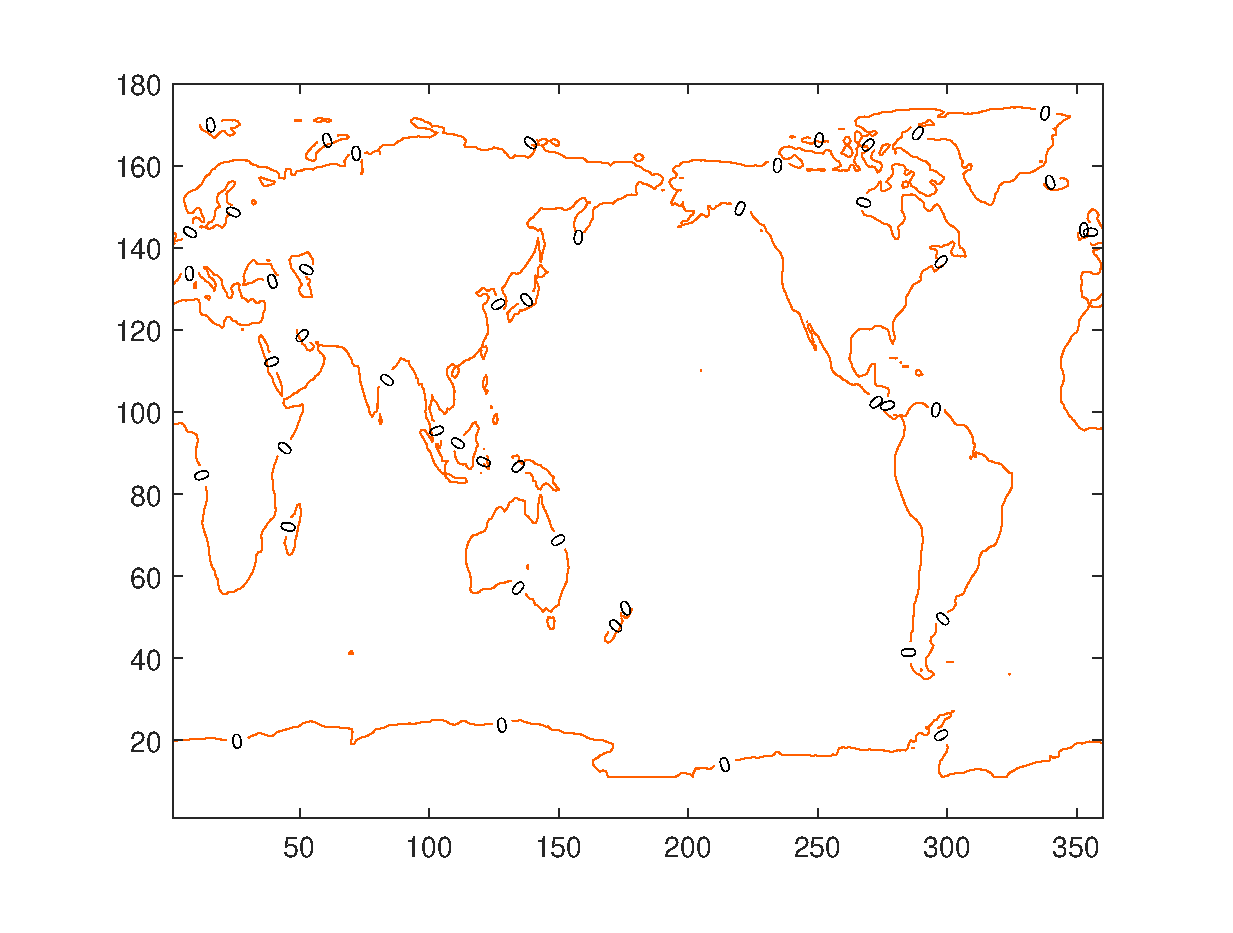
\includegraphics[width=\linewidth]{ch5-contour4.eps}
\caption{Example usage of \texttt{contour}, contouring only the zero height isoline, and providing a label.}
\label{fig:ch5-contour4}
\end{marginfigure}

If you do this, in an earlier example of plotting just the zero height contour, and now using the most basic default usage of \texttt{clabel} (as above), you get, for good or for bad, Figure \ref{fig:ch5-contour4}.

In the default usage of \texttt{clabel}, you'll get a label added on every contour that you plot. This ... can get kinda messy if you have lots and lots of contours plotted. You may well not need every single contour labelled, particularly if you also provide a color scale (see below). So you can also pass in a vector to tell \textbf{MATLAB} which contours to label. For example, if you have a contour interval vector:
\begin{docspec}
v = [-1000:100:1000];
\end{docspec}
(which creates 100 m spaced contours between -1000 and +1000 m) maybe you only want labels on contours every 500m, so you'd create a \uline{different} vector:
\begin{docspec}
w = [-1000:500:1000];
\end{docspec}
to specify the labelling intervals. The complete set of commands for this becomes:
\begin{docspecbold}
>> v = [-1000:100:1000];
\\ >> w = [-1000:500:1000];
\\ >> [C,h] = contour(etopo1deg,v);
\\ >> clabel(C,h,w);
\end{docspecbold}
where \texttt{[C,h] = contour(etopo1deg,v);} specifies to contour from -1000 to 1000 in steps of 100,\texttt{ but clabel(C,h,w);} says to label only every 500 m (from -1000 to 1000).

Finally -- missing from our color-coded plots so far, is a color scale to relate values to colors (although labelling the contours works as an OK substitute). The \textbf{MATLAB} command is as simple as typing:
\begin{docspecbold}
>> colorbar
\end{docspecbold}
(and see Box for further usage). Try adding a \textit{colorbar}, and in different places in the plot. Refer to the Box to try and add a caption to it ...

\marginnote[-4.75in]{\begin{mdframed}[backgroundcolor=gray!10, roundcorner=10pt,leftmargin=1, rightmargin=1, innerleftmargin=5, innerrightmargin=5, innertopmargin=5,innerbottommargin=5, outerlinewidth=1, linecolor=light-gray]
\docenvdef{colorbar}
\\This almost could not be simpler:
\begin{docspecmargin}
>> colorbar
\end{docspecmargin}
plots the color scale! By default, is places it to the RH sice of the plot. If you wish for it to appear anywhere else, use the modified syntax:
\begin{docspecmargin}
>> colorbar(PLACEMENT)
\end{docspecmargin}
where PLACEMENT is one of: \texttt{'northoutside'}, \texttt{'southoutside'}, \texttt{'eastoutside'}, \texttt{'westoutside'}. Note that these are strings and so need to be in quotation marks. (More options are summarized in a table in \textbf{help}.)
\\Finally, you can also add a label to the \textit{colorbar}, but only if you get hold of its ID ('graphics handle') when you call \texttt{colorbar}, e.g.
\begin{docspecmargin}
>> h = colorbar
\end{docspecmargin}
will save the graphics handle in variable \texttt{h}, which you can then muck about with via:
\begin{docspecmargin}
c.Label.String = 'The units of my lovely colorbar';
\end{docspecmargin}
(Don't fight this -- use this syntax to set a label for the \textit{colorbar} -- don't worry about  what it means. \textbf{MATLAB} keeps rather annoyingly changing the way it does this anyway :()
\end{mdframed}}

%------------------------------------------------
%
\newpage
\subsection{Meshgrid}

We'll now address the issue with missing/incorrect lon/lat axis labels on the plots.

Each data point in the \texttt{etopo1deg} matrix should have one longitude value (\textit{x}-axis) and one latitude (\textit{y}-axis) value associated with it. What we need, is a pair of matrices, of exactly the same size as the \texttt{etopo1deg} data matrix -- one holding longitude values and one latitude values.

There are various ways of creating the required matrices 'by hand' (or involving writing a program including a \textit{loop}). All of them are tedious. There is a \textbf{MATLAB} function to help. But it is not entirely intuitive\sidenote[][-0.0in]{\textbf{\textcolor{red}{DON'T\ PANIC!}}} ... \docenv{meshgrid}.

\marginnote[-0.0in]{\begin{mdframed}[backgroundcolor=gray!10, roundcorner=10pt,leftmargin=1, rightmargin=1, innerleftmargin=5, innerrightmargin=5, innertopmargin=5,innerbottommargin=5, outerlinewidth=1, linecolor=light-gray]
\docenvdef{meshgrid}
\\The unholy syntax is:
\begin{docspecmargin}
[X,Y] = meshgrid(xv,yv)
\end{docspecmargin}
Pause, and take a deep breath. On the left -- the results of \texttt{meshgrid} are being returned to 2 matrixes, \texttt{X} and \texttt{Y}. These are going to be our matrixes of the longitude and latitude values (in the particular example in the text). So far so good(?)
\\On the right, passed into the function \texttt{meshgrid}, are two vectors -- \texttt{xv} and \texttt{yv}. Pause again.
\\What \textbf{MATLAB} is going to do, is to take the (row) vector \texttt{xv}, and it is going to replicate it down so that there are as many rows as in the vector \texttt{yv}. This becomes the returned output matrix \texttt{X}. \textbf{MATLAB} then takes the column vector \texttt{yv}, and replicates it across so that there are as many columns as in the vector \texttt{xv}. This becomes the returned output matrix \texttt{Y}.
\end{mdframed}}

Spend a few minutes reading about it in \texttt{help}. In particular, look at the examples given to help you translate the \textbf{MATLAB}-speak gobbledegook of the function description. You should be able to glean from all this that this \textit{function} allows us to create two \(a\times b\) arrays; one with the columns all having the same values, and one with the rows all having the same values (exactly what we need for defining the (lon,lat) of all the global data points). If not, and probably not -- see Box. And then lets do a simple example (adapted from \textbf{help}) (at the Command line):
\begin{docspecbold}
>> [X,Y] = meshgrid(1:3,10:14)
\end{docspecbold}
\begin{docspec}
X =
\\ \ \ \ \ 1     2     3
\\ \ \ \ \ 1     2     3
\\ \ \ \ \ 1     2     3
\\ \ \ \ \ 1     2     3
\\ \ \ \ \ 1     2     3
\\Y =
\\ \ \ \ \ 10    10    10
\\ \ \ \ \ 11    11    11
\\ \ \ \ \ 12    12    12
\\ \ \ \ \ 13    13    13
\\ \ \ \ \ 14    14    14
\end{docspec}
Here, we are taking 2 vectors -- \texttt{[1:3]} and \texttt{[10:14]}, and asking \textbf{MATLAB} (very nicely) to create 2 matrixes, one in which \texttt{[1:3]} is replicated down, until it has the same number of rows as the length of \texttt{[10:14]}, and one in which \texttt{[10:14]} is replicated across until it has the same number of columns as the length of \texttt{[1:3]}.

In our example 2D (topography) dataset -- start by noting that the topography data is on a regular 1 degree grid starting at 0\degree\ longitude. Latitude starts (at the bottom) at -90\degree\ and goes up to +90\degree\ . We need a matrix containing all the longitude values from 0\degree\ to 359\degree\, and latitude from -90\degree\ to 89\degree\ .\sidenote{There is a slight complication with this, which we'll get to shortly, but note that the data array is 360 elements (\textit{x}-direction) by 180 elements (\textit{y}-direction).} These matrices need to be the same size as the data matrix.

Maybe just go ahead and do it right now ... and then pause and understand what has happened after. Create the longitude and latitude grids by:
\begin{docspecbold}
>> [lon lat] = meshgrid([0:359],[-90:89]);
\end{docspecbold}

View (in the \textsf{Variables window}) the \texttt{lon} matrix first. Scan through it. Hopefully ... you'll note that it is 360 columns across, and in each column has the same value -- the longitude. The matrix is 180 rows 'high', so that there is a longitude value for each latitude. Similarly, view \texttt{lat}. This also should make a little sense if you pause and think about it, with the one exception that the South Pole latitude is at the 'top' of the matrix -- don't worry about this for now ... 

The only way to fully make sense of things now, is to use it. Remember that use of \texttt{contour} (and \texttt{contourf}) can take matrices of \textit{x} and \textit{y} (here: longitude and latitude) values that correspond to the data entries in the data matrix (\texttt{etopo1deg}). 

Re-load the topography data in case you have flipped it about in all sorts of odd ways, and then do:
\begin{docspecbold}
>> [lon lat] = meshgrid([0:359],[-90:89]);
\\ >> contour(lon,lat,etopo1deg);
\end{docspecbold}
Almost! Note that the \textit{x} and \textit{y} axis labelling is 'correct' and particularly the \textit{y}-axis, where latitude goes from -90 to 90 (although by default \textbf{MATLAB} labels in intervals of 20 starting at -80 it seems). But it also turns out that we do need to flip the data up-side-down. We can actually do this in the same line as we plot:
\begin{docspecbold}
>> contour(lon,lat,flipud(etopo1deg));
\end{docspecbold}
or if you prefer 2 explicit steps:
\begin{docspec}
>> etopo1deg\_corrected = flipud(etopo1deg);\\
>> contour(lon,lat,etopo1deg\_corrected);
\end{docspec}

Phew! (Figure Figure \ref{fig:ch5-contour5}.)

\begin{marginfigure}[0.0in]
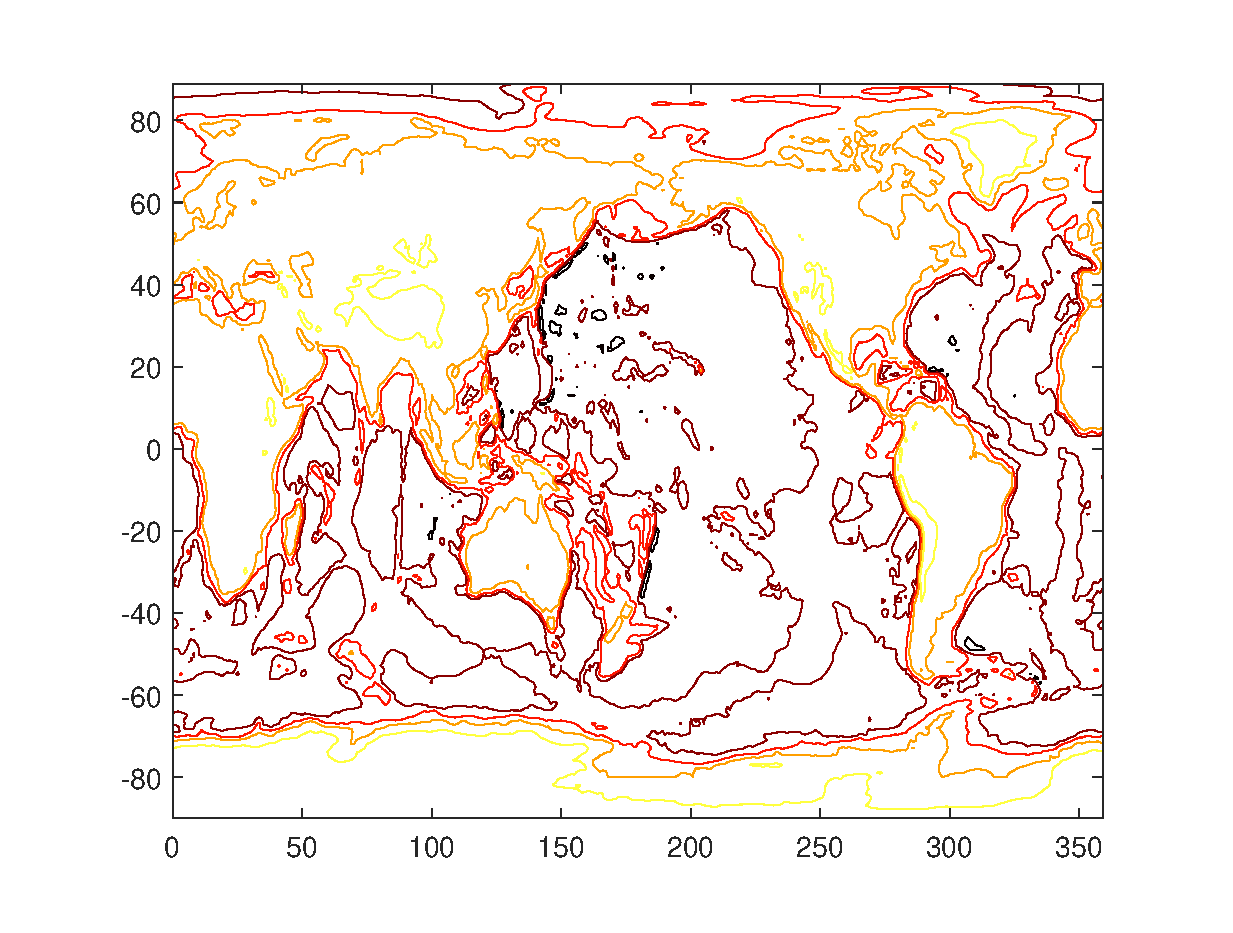
\includegraphics[width=\linewidth]{ch5-contour5.eps}
\caption{Usage of \texttt{contour} but with lon/lat values created by \texttt{meshgrid} function and passed in (and with the \texttt{hot} \textit{colormap} (giving dark/brown colors as deep ocean, and light/white as high altitude).}
\label{fig:ch5-contour5}
\end{marginfigure}

The final complication is that the data points in the gridded dataset (matrix \texttt{etopo1deg}), technically correspond to the mid-points of a 1 degree grid, not the corners. So if we were going to try and be formally correct\sidenote{Don't worry about this for now -- grids will be covered more in subsequence chapters surrounding numerical (environmental) models.}, our vectors that we'd pass into \texttt{meshgrid}, would be:
\begin{docspec}
>> x = [0.5:359.5];
\\ >> y = [-89.5:89.5];
\end{docspec}
and hence:
\begin{docspec}
>> [lon lat] = meshgrid(x,y);\\
>> contour(lon,lat,flipud(etopo1deg));
\end{docspec}

%------------------------------------------------

\vspace{1mm}
\noindent\rule{4cm}{0.5pt}
\vspace{-2mm}

%------------------------------------------------

\newthought{[\textbf{\textcolor{red}{OPTIONAL}}] Another Example} on this. Previously, you downloaded and plotted monthly global distributions of surface air temperature. You plotted these simply using \texttt{pcolor} (or \texttt{image}) and the results were ... variable. Certainly not publication-quality graphics and missing appropriate longitude and latitude axes for the plots.

Make a copy of your original \textit{script} (\textsf{m-file}) in which you created the animation, and give it a new name. Edit your program, and in place of \texttt{pcolor}, use \texttt{contour} or \texttt{contourf} (your choice!). To begin with, pass in just the data matrix (of monthly temperature) when calling the \texttt{contour} (or \texttt{contourf}) function and don't yet worry about the lon/lat values. Get this working (i.e. debug it if not). You should end up with a contoured animation (rather than a bit-map animation).

The problem with the axis labelling should be much more apparent (than compared to the topography data, which was on a handy 1 degree grid already). So you need to make a matrix of longitude values, and one of latitude. using \texttt{meshgrid}. The grid is a little awkward:
\begin{enumerate}[noitemsep]
\setlength{\itemindent}{.2in}
\item The longitude grid runs from 0\degree E (column \#1) with an increment of 1.875\degree ; i.e., 0.000\degree E, 1.875\degree E, 3.750\degree E, ... up to 358.125\degree E (column \#192).
\item Latitude runs from 88.54196\degree S (-88.54196\degree N) at row \#1, to 88.54196\degree N (row \#94) with an increment of about 1.904.
\end{enumerate}
so I'll give you the answer up-front:
\begin{docspecbold}
 \ lonv = [(1.875/2):1.875:360-(1.875/2)];
\\ \ latv = [-90+(1.904/2):1.904:90-(1.904/2)];
\\ \ [lon lat] = meshgrid(lonv,latv);
\end{docspecbold}
Place this code somewhere \uline{before} the loop starts in your program.

Now use the longitude and latitude values matrices, in conjunction with \texttt{contour}(\texttt{f}), to plot the global temperature distributions 'properly', e.g.
\begin{docspecbold}
contour(lonv,latv,temp);
\end{docspecbold}
or if you prefer:
\begin{docspec}
contour(lonv(:,:),latv(:,:),temp(:,:));
\end{docspec}
and it helps you remember which variables are arrays.

Try plotting just one plot first (e.g. by adding a breakpoint at the end of the loop, i.e. the line with \texttt{end}), before looping through all 12 months. 

At this point (before creating an animation), you might also explore some of the plotting refinements we saw earlier. For example, as per Figure \ref{fig:ch5-contour6}. 
Firstly -- get the units of the temperature data array into units of \degree C (or \degree  F if you are into that sort of thing) rather than \degree K. Either: assign the \texttt{temp} array data to a new array and make the appropriate conversion from \degree K (all within the loop), or you can do this subtraction on the line that you actually plot the data (i.e., within the \texttt{contour}/\texttt{contourf} function), for example:
\begin{docspec}
contourf(lon(:,:),lat(:,:),temp(:,:)-273.15);
\end{docspec}
\noindent would convert to \degree C as it plotted the data.

\begin{marginfigure}[0.0in]
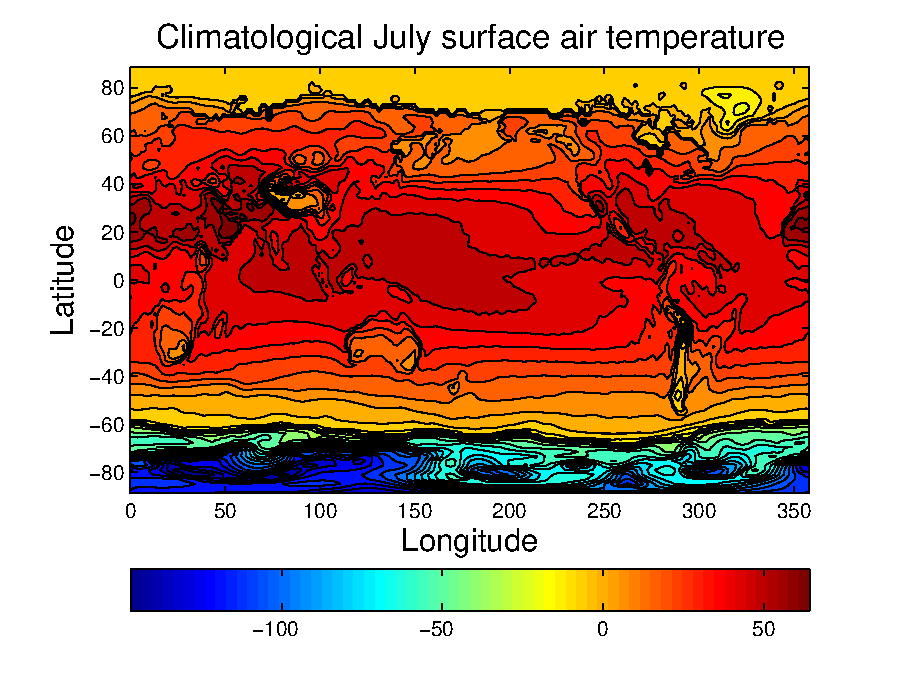
\includegraphics[width=\linewidth]{ch5-contour6.eps}
\caption{Example contour plot including \texttt{meshgrid}-generated lon/lat values. Result of \texttt{contourf(lon,lat,temp7,30)}, where the data file was \texttt{temp7.tsv}, with some embellishments.}
\label{fig:ch5-contour6}
\end{marginfigure}

You can also (assuming you converted to units of \degree C) set the plotting temperature limits and contouring consistent between months and with greater color interval resolution by adding the following line (before the loop starts):
\begin{docspecbold}
v=[-40:2:40];
\end{docspecbold}
\noindent and then to the \texttt{contour(...)} (or \texttt{contourf(...)}) function, add to the end of the list of passed parameters -- \texttt{v}, e.g.
\begin{docspec}
contourf(lon(:,:),lat(:,:),temp(:,:),v);
\end{docspec}

This particular choice for the vector \texttt{v} tells \textbf{MATLAB} to do the contouring from -40 to 40 (\degree C), and at a contour interval of 2 (\degree C).. Play around with the min and max limits of the range, and also with the contour interval to see what gives the clearest and least cluttered plot. For instance, maybe you don't want the low temperatures to go 'off' the scale (the white color in the filled contour plot).

%------------------------------------------------

\vspace{1mm}
\noindent\rule{4cm}{0.5pt}
\vspace{2mm}

\noindent Lastly -- for any (or all) of the Examples above, you could add the continental outline to the plot. Remember, to use \texttt{hold on} in order to overlay the continental outline on top of the contour map without replacing it in the \textsf{Figure window}.

It should be obvious that plotting the continental outline might be something you want to us more than once. Sections of code that might get used multiple times are commonly placed in a file (or special section of the file) of their own and \textit{called} from the main program that needs it. For example, you could place the entire continental outline plotting code, including loading in the data, in an \textsf{m-file} and make it a \textit{function} -- in this case, taking no parameters as input, and return no output.\sidenote[][-2.0in]{Make sure that you do not open a figure window with the \texttt{figure} command with the function, or you will not get a continental output overlay on your plot, but rather a sperate \textsf{Figure window} with just the continental outline on.} In the example of the looped animation, in the sequence of code (within the loop), you will need to \textit{call} your continental outline plotting function just after you have plotted the contour (or bitmap) plotting function.

%------------------------------------------------

\marginnote[-1.75in]{\begin{mdframed}[backgroundcolor=gray!10, roundcorner=10pt,leftmargin=1, rightmargin=1, innerleftmargin=5, innerrightmargin=5, innertopmargin=5,innerbottommargin=5, outerlinewidth=1, linecolor=light-gray]
\textbf{The MATLAB Mapping toolbox}
\\You can do some nice spatial plotting with this data using the \textbf{MATLAB} \textsf{Mapping Toolbox}. This should be available as part of the \textbf{MATLAB} installation in the Lab (and also if you have downloaded and installed an academic version on a personal laptop). Refer to the on-line documentation for the \textsf{Mapping Toolbox} to get you started. The key function appears to be \docenv{geoshow}. Try plotting the region encompassing the 'quake data, with a coastal outline (of land masses), and the 'quake data overlain. Explore different map projections. Remember to always ensure appropriate labelling of plots.
\end{mdframed}}

%------------------------------------------------

\newpage

%------------------------------------------------

\section{Further data processing}

This section contains a selection of further simple techniques for doing useful stuff with data, as well as for better graphing.

%------------------------------------------------
%
\newpage

%------------------------------------------------

\subsection{\texttt{find}!}

So -- a single \textbf{MATLAB} function gets its own sub-section, all to itself. Either it's really powerful and useful, or I am running out of ideas for the textbook\sidenote{Answer: it is really powerful and useful.}.

\marginnote{\begin{mdframed}[backgroundcolor=gray!10, roundcorner=10pt,leftmargin=1, rightmargin=1, innerleftmargin=5, innerrightmargin=5, innertopmargin=5,innerbottommargin=5, outerlinewidth=1, linecolor=light-gray]
\docenvdef{find}
\\\textbf{MATLAB} defines find, with a basic syntax of:
\begin{docspecmargin}
k = find(X)
\end{docspecmargin}
as '\textit{return[ing] a vector containing the linear indices of each nonzero element in array X}'.
\\That means ... nothing to me. This is going to have to be a job for some Examples ... (in order to see what \docenv{find} is all about).
\\ Actually, \texttt{find} returns the indices of the non-zero elements in the array and if the array is a vector, what is does is simple. For a matrix, \textbf{MATLAB} counts the elements sequentially, starting at the 1st row and 1st column, and working down the first column, rather than provide the (row,column) for indexing format you are used to. Hence where the '\textit{linear indices}' bit comes in.
\\ Furthermore, 'non-zero' indices is really just code-word for 'true'. So you are asking where the true values occur in \texttt{X}. If \texttt{X} is the answer to a \textit{logical} or \textit{relational} operation, then find tells you the indices of the elements that are true.
\\ For example, \texttt{3 > [5 3 1]} equates to \texttt{[0 0 1]}, i.e. only the first element in the vector \texttt{[5 3 1]} is less than \texttt{3}. Hence:
\begin{docspecmargin}
find(3 > [5 3 1])
\end{docspecmargin}
first evaluates the relational operation and generates a vector of true and false values, and then \texttt{find} tells you the index (or indices) where the true values occur (here, \texttt{ans = 3}).
\end{mdframed}}

\marginnote{\begin{mdframed}[backgroundcolor=gray!10, roundcorner=10pt,leftmargin=1, rightmargin=1, innerleftmargin=5, innerrightmargin=5, innertopmargin=5,innerbottommargin=5, outerlinewidth=1, linecolor=light-gray]
\docenvdef{min}
\\\noindent\docenvdef{max}
\\Return the minimum and maximum, respectively, values in an array. e.g.
\begin{docspecmargin}
min([4 8 3 1])
\end{docspecmargin}
will return a value of \texttt{1}.
\end{mdframed}}

\docenv{find} ... finds where-ever in an \textit{array}, a specific condition is met. If the specific condition occurs once, a single \textit{array} location is returned. The specific condition could occur multiple times, in which case \texttt{find} will report back multiple positions in the \textit{array}.

What do I mean by a 'specific condition'? Basically -- exactly as per in the \texttt{if ...} construction -- a \textit{conditional} statement being evaluated to \textit{true}.

OK -- some  Examples.

Say that you have a \textit{vector} of numbers, e.g.:
\begin{docspec}
A = [3 7 5 1 9 7 4 2];
\end{docspec}
and you want to find the maximum value in the vector -- easy\sidenote{I hope so ... check back earlier (or slightly later) in the course on \texttt{max}.}.

But ... perhaps you want to find *where* in the vector the maximum value occurs. Why might you want to do this? Rarely do you have a single vector of data on its own -- generally it is always linked to at least one other vector (often time or length in scientific examples). Trivially, our second vector might be:
\begin{docspec}
B = [0:7];
\end{docspec}
and represent, for instance, time. The question then becomes: at what time did the maximum value occur? Obviously, this is easy by eye with just 8 numbers, but if you had 1000s ...

We can start by determining the maximum value (in the  array, \texttt{A}).
\begin{docspec}
c = max(A);
\end{docspec}

Now, we use \docenv{find} to evaluate \uline{where} (what index) in  array \texttt{A} the element with a value of \texttt{max(A)} (equal to \texttt{c}) occurs. The following should accomplish this:
\begin{docspec}
find(A(:)==c);
\end{docspec}

Here, what we are saying is: take all of the elements in \texttt{A} and \uline{find} where an element occurs that is equal to \texttt{c} (the maximum value, which we already determined). Try it, and \textbf{MATLAB} should return \texttt{5} -- the 5th element in the vector.

Finally, if we assign the result of \texttt{find} to \texttt{d}, remembering that \texttt{find} return an array index (or indices), we can then use \texttt{d} to determine the time at which the value of \texttt{9} occurred, i.e. \texttt{B(d)} which evaluates to \texttt{4} (whatever units of time):
\begin{docspec}
d = find(A(:)==c);\\
B(d)
\end{docspec}

In this example, \docenv{find} returned just a single element, but if we instead had:
\begin{docspec}
A = [3 9 5 1 9 7 4 2];
\end{docspec}
The maximum value is still the same (\texttt{9}) but now you get ...
\begin{docspec}
>> find(A(:)==c)\\
ans =
\\ \ \ \ \ 2
\\ \ \ \ \ 5
\end{docspec}

What has happened is that \docenv{find} has determined that there are 2 elements in vector \texttt{A} that satisfy the condition of being equal to \texttt{c} (\texttt{9}) and that these lie at positions (index) \texttt{2} and \texttt{5}. The resulting \textit{vector}, if you assigned it to the variable \texttt{d} again, can be used just as before to access the corresponding times in vector \texttt{B};
\begin{docspec}
>> d = find(A(:)==c);\\
>> B(d)
\\ans =
\\ \ \ \ \     1     4
\end{docspec}
i.e. that the times at which the values of \texttt{9} occur are \texttt{1} and \texttt{4} (whatever units).

Any of the \textit{relational operators} (that evaluate to \textit{true} or \textit{false}) can be used. In fact -- looking at it this way leads us to maybe understand the \textbf{MATLAB} \textbf{help} text, because \textit{true} and \textit{false} are equivalent to \texttt{1} and \texttt{0}, and \texttt{find} is defined as a function that returns the indices of the non-zero elements in a \textit{vector}. By writing \texttt{A(:)==c} we are in effect creating a vector of \texttt{1}s and \texttt{0}s depending on whether the equality is \textit{true} or not for each element. You can pick apart what is going on and see that this is the case, by typing:
\begin{docspecbold}
>> A(:)==c
\\ans =
\\ \ \ \ \ 0
\\ \ \ \ \ 1
\\ \ \ \ \ 0
\\ \ \ \ \ 0
\\ \ \ \ \ 1
\\ \ \ \ \ 0
\\ \ \ \ \ 0
\\ \ \ \ \ 0
\end{docspecbold}
(the statement being \textit{true} at positions (index) \texttt{2} and \texttt{5}, which is exactly what \texttt{find} told you).

As another example, we could ask \texttt{find} to tell us which elements of A have a value greater than 5:
\begin{docspecbold}
>> find(A(:)>5)
\\ ans =
\\ \ \ \ \ 2
\\ \ \ \ \ 5
\\ \ \ \ \ 6
\end{docspecbold}
(Inspect the contents of vector \texttt{A} and satisfy yourself that this is the case.)

We can also use \texttt{find} to filter data. Perhaps you do not want values over 5 to remain in the dataset. Perhaps this is above the maximum reliable range of the instrument that generated them or whatever reason. Having obtained a vector of locations of these values, e.g.
\begin{docspec}
d = find(A(:)>5);
\end{docspec}
we can plug this vector back into \texttt{A} and assign arrays of zero size to these locations -- effectively, deleting the locations in the array, i.e.
\begin{docspec}
A(d) = [];
\end{docspec}
Note that the size\sidenote{Use the command \texttt{length} or view in the \textsf{Workspace Window}.} of \texttt{A} has now shrunk to \texttt{5} -- all the other elements remain, and in order, but the elements with a value greater than 5 have gone. You could apply an identical deletion (filtering) to the time array (\texttt{B(d) = []}).

Play about with some other relational operators and criteria, and make up some vectors of your own until you are comfortable with using \texttt{find}. 
%------------------------------------------------

\vspace{1mm}
\noindent\rule{4cm}{0.5pt}
\vspace{-2mm}

%------------------------------------------------

\newthought{For an Example of data-filtering} -- dig out the paleo-proxy (\texttt{paleo\_CO2\_data.txt}) atmospheric CO\(_{2}\) data you downloaded earlier. One further way of plotting with \texttt{scatter} is to scale the point size by a data value. We could do with by:
\begin{docspecbold}
>> SCATTER(data(:,1),data(:,2),data(:,2))
\end{docspecbold}
... except ... it turns out that there are atmospheric CO\(_{2}\) estimates of zero or less   and \texttt{scatter} will refuse to scale the point size by such values ...

\marginnote{\begin{mdframed}[backgroundcolor=gray!10, roundcorner=10pt,leftmargin=1, rightmargin=1, innerleftmargin=5, innerrightmargin=5, innertopmargin=5,innerbottommargin=5, outerlinewidth=1, linecolor=light-gray]
\docenvdef{NaN}
\\... is \textbf{Not-a-Number} and is a representation for something that cannot be represented as a number, although if you try and divide something by zero \textbf{MATLAB} reports \texttt{Inf} rather than a \texttt{NaN}.
\\ \texttt{NaN} can also be used as a function to generate arrays of \texttt{NaN}s. The most common/usage in this context is:
\begin{docspecmargin}
N = NaN(sz1,...,szN)
\end{docspecmargin}
which will (according to \textbf{help}) "generate a a sz1-by-...-by-szN array of NaN values where sz1,...,szN indicates the size of each dimension. For example, \texttt{NaN(3,4)} returns a 3-by-4 array of NaN values."
\end{mdframed}}

This leads us to a new use for \docenv{find} and some basic data filtering. We'll start by tackling the zeros.

 The simplest thing you could do to ensure that no zero value appear anywhere, would be to add a very small number to all the values. This would defeat the 'no zero' parameter restriction, but would not help if there were negative values and you have now slightly modified and distorted the data which is not very scientific. Substituting a \docenv{NaN} for problem values is a useful trick, as \textbf{MATLAB} will simply ignore and not attempt to plot such values.

So first, lets replace any zero in the CO\(_{2}\) column of the data with a \texttt{NaN}. The compact version of the command you need is:
\begin{docspec}
data(find(data(:,2)==0),2)=NaN;
\end{docspec}
But as ever -- perhaps break this down into separate steps and use additional arrays to store the results of intermediate steps, if it makes it easier to understand, e.g.
\begin{docspecbold}
>> list\_of\_zero\_locations = find(data(:,2)==0);
\\>> data(list\_of\_zero\_locations,2) = NaN;
\end{docspecbold}
What this is saying is: first find all the locations (row indices) in the 2nd column of \texttt{data} for which the value is equivalent (\texttt{==}) to zero. Then, replace the CO\(_{2}\) value in all these rows of the 2nd column (which is originally zero) with a \texttt{NaN} (technically speaking: assign a value of \texttt{NaN} to these locations). 

You have now filtered out zeros, and replaced the offending values with a \texttt{NaN} and when \textbf{MATLAB} encounters \textit{NaNs} in plotting -- it ignores them and omits that row of data from the plot.
 
Alternatively, we could have simply deleted the entire row containing each offending zero.\footnote{\uline{First}: Re-load  the paleo-proxy atmospheric CO\(_{2}\) data so that you can have another go at filtering it.} Breaking it down, this is similar to before in that you start by identifying the row numbers of were zeros appear in the 2nd column, but now we set the entire row to be 'empty', represented by \texttt{[]}:
\begin{docspecbold}
>> list\_of\_zero\_locations = find(data(:,2)==0);
\\ >> data(list\_of\_zero\_locations,:) = [];
\end{docspecbold}
If you check the \textsf{Workspace window}\sidenote{Or: \\\texttt{>> size(data)}}, you should notice that the size of the array data has been reduced (by 4 rows, which was the number of times a zero appeared in the 2nd column).

We are almost there with this example except it turns out that there is a CO\(_{2}\) proxy data value less than zero(!!!) We can filter this out, just as for zeros. I'll leave this as an exercise for you -- remember the operator 'less than' (\texttt{<}).\sidenote{Actually, you could have done the filtering of both zeros, and values less than zero, all in one, using: \(\leq\)}

The plot should end up looking like Figure \ref{fig:plot-CO2scatter3}. As another lesson-ette, given that the circles are insanely large ... you might try plotting this with proportionally smaller circles, which you could achieve by e.g.
\begin{docspecbold}
>> SCATTER(data(:,1),data(:,2),0.5*data(:,2))
\end{docspecbold}
which simply make the 2nd column values passed to \texttt{scatter} to set the marker size, to half their original value.

\begin{marginfigure}[0.0in]
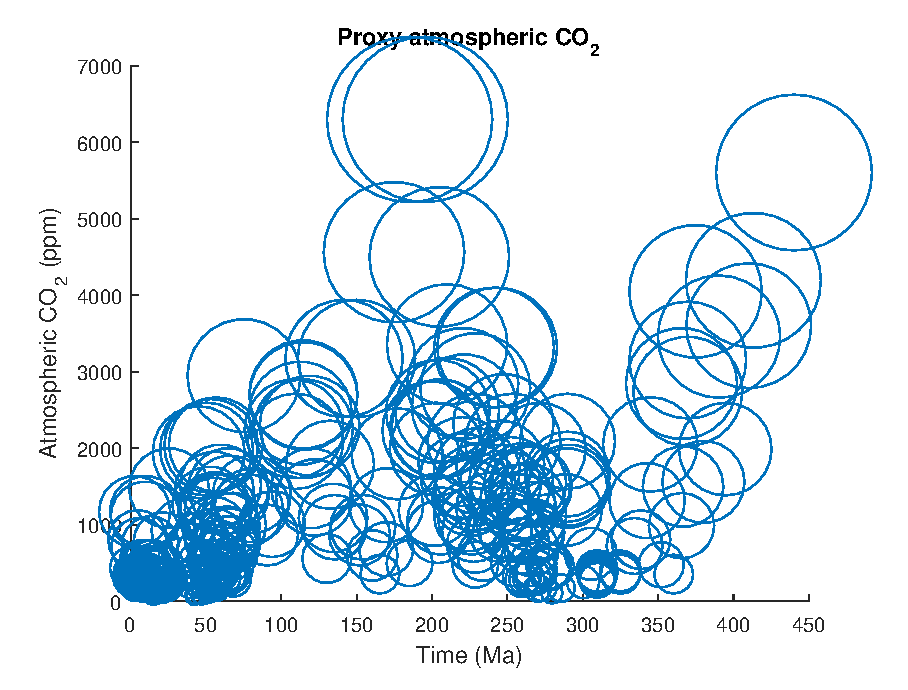
\includegraphics[width=\linewidth]{plot-CO2scatter3.eps}
\caption{Proxy reconstructed past variability in atmospheric CO2 (scatter plot).}
\label{fig:plot-CO2scatter3}
\end{marginfigure} 

\vspace{1mm}
\noindent\rule{4cm}{0.5pt}
\vspace{2mm}

\noindent Having inserted \texttt{NaN}s into an array, or having ended up with \texttt{NaN}s in an array for other reasons, you can also search for (\texttt{find}) the \texttt{NaN}s.
The first thing to note in looking for \texttt{NaN}s, is you cannot test for a \texttt{NaN} with a simple equality operator:
\begin{docspecbold}
>> a=NaN;\\
>> a==NaN\\
ans =\\
\ \ \ 0
\end{docspecbold}
which ... is odd. Having assigned a \texttt{NaN} to variable \texttt{a} (first line), \textbf{MATLAB} is apparently telling you that the value of \texttt{a} is not equivalent to \texttt{NaN}.
Really unhelpful.
In fairness, \texttt{a} does not have a value and is Not A Number and hence \textbf{MATLAB} cannot determine whether or not it is equal to another Not A Number.
 Better would have been for \textbf{MATLAB} to give you an error ... still, it is what it is.

To try and make amends, \textbf{MATLAB} provides a \textit{function} to determine whether or not something is Not A Number -- \docenv{isnana}. This returns \textit{true} (\texttt{1}) if the passed variable is Not A Number, and \textit{false} (\texttt{0}) if not, e.g.

\marginnote[-1.5in]{\begin{mdframed}[backgroundcolor=gray!10, roundcorner=10pt,leftmargin=1, rightmargin=1, innerleftmargin=5, innerrightmargin=5, innertopmargin=5,innerbottommargin=5, outerlinewidth=1, linecolor=light-gray]
\docenvdef{isnan}
\\'\textit{\texttt{isnan(A)} returns an array the same size as \texttt{A} containing logical \texttt{1} (true) where the elements of \texttt{A} are \texttt{NaN}s and logical \texttt{0} (false) where they are not.}'
\\Meaning that you can pass any dimension of array (e.g. vector or matrix or 3D), not just a scalar (a single value or \(1\times1\) matrix). 
\end{mdframed}}
\begin{docspecbold}
>> isnan(a)\\
ans =\\
\ \ \ 1
\end{docspecbold}
(because we set \texttt{a} to \texttt{NaN} earlier), whereas:
\begin{docspecbold}
>> isnan(99)\\
ans =\\
\ \ \ 0
\end{docspecbold}
because \texttt{99} is a number (integer) and not a Not A Number.

\vspace{1mm}
\noindent\rule{4cm}{0.5pt}
\vspace{-4mm}

\subsection{Other data filtering}

\noindent In the example of the observational Riverside temperature data (the data file: \texttt{temperature\_riverside.txt}), if would be nice to also be able to use \docenv{find} ... which can  determine all the locations at which a \texttt{NaN} occurs\sidenote{Using \docenv{isnan}.}, by e.g.:
\begin{docspec}
>> find(isnan(temperature\_riverside))
\end{docspec}

\noindent ... but it is not obvious what to 'do' with the resulting list of \textit{linear indices} for each cell containing a missing value (\texttt{NaN}). For instance, you cannot remove a single cell from a \(a\times b\) array because an array must contain the same number of elements in each row and the same number of elements in each column.

What you need, is a way of automatically removing each and every row in which one (or more) \texttt{NaN}s appear. There are two obvious approaches:

\vspace{2mm}
\textbf{1. use a loop}
\vspace{2mm}

\noindent We could go through the array, row by row, and for every row in which a \texttt{NaN} occurs, remove that row. The code (in a new \textit{script} file) could look something like the following and which works ... but maybe is a little complicated and/or contorted:

\begin{docspec}
\textcolor[rgb]{0,0.501961,0}{\%\%\% script to load data, remove NaN-containing rows}\\
\textcolor[rgb]{0,0.501961,0}{\% load dataset}\\
data=load(\textcolor[rgb]{1,0,1}{'temperature\_riverside.txt'});\\
\textcolor[rgb]{0,0.501961,0}{\% determine number of rows of data}\\
n\_max = length(data);\\
\textcolor[rgb]{0,0.501961,0}{\% initialize row count to the first row}\\
n = 1;\\
\textcolor[rgb]{0,0.501961,0}{\% loop through all rows}\\
\textcolor{blue}{while} (n <= n\_max),\\
\ \ \ \textcolor[rgb]{0,0.501961,0}{\% find all (any) NaNs in current row}\\
\ \ \    found\_nans = find(isnan(data(n,:)));\\
\ \ \ \textcolor[rgb]{0,0.501961,0}{\% did you find any NaNs?}\\
\ \ \ \textcolor[rgb]{0,0.501961,0}{\% the vector found\_nans is not empty if you did!}\\
\ \ \    \textcolor{blue}{if} (\(\sim\)isempty(found\_nans));\\
\ \ \ \ \ \        \textcolor[rgb]{0,0.501961,0}{\% then remove entire row}\\
\ \ \ \ \ \        data(n,:) = [];\\
\ \ \ \ \ \        \textcolor[rgb]{0,0.501961,0}{\% remember to update total number of rows!!!}\\
\ \ \ \ \ \        \textcolor[rgb]{0,0.501961,0}{\% (there is one less now)}\\
\ \ \ \ \ \        n\_max = n\_max - 1;\\
\ \ \ \ \ \        \textcolor[rgb]{0,0.501961,0}{\% NOTE: don't update row count}\\
\ \ \    \textcolor{blue}{else}\\
\ \ \ \ \ \        \textcolor[rgb]{0,0.501961,0}{\% move on to next row}\\
\ \ \ \ \ \        n = n+1;\\
\ \ \    \textcolor{blue}{end}\\
\textcolor{blue}{end}\\
\end{docspec}

\vspace{2mm}
\textbf{2. cheat!}
\vspace{2mm}

(not really)

\noindent There is a relatively new \textbf{MATLAB} \textit{function} that achieves just this: \docenv{rmmissing} (see Box). Much simpler  code that does exactly the same job as above, would then look like:
\begin{docspec}
\textcolor[rgb]{0,0.501961,0}{\%\%\% script to load data, remove NaN-containing rows}\\
\textcolor[rgb]{0,0.501961,0}{\% load dataset}\\
data=load(\textcolor[rgb]{1,0,1}{'temperature\_riverside.txt'});\\
\textcolor[rgb]{0,0.501961,0}{\% remove problem rows!!!}\\
data = rmmissing(data);
\end{docspec}

\marginnote[-1.625in]{\begin{mdframed}[backgroundcolor=gray!10, roundcorner=10pt,leftmargin=1, rightmargin=1, innerleftmargin=5, innerrightmargin=5, innertopmargin=5,innerbottommargin=5, outerlinewidth=1, linecolor=light-gray]
\docenvdef{rmmissing} -- 'Remove rows or columns with missing entries'.
\\In the simplest usage:
\begin{docspecmargin}
B = rmmissing(A);
\end{docspecmargin}
Removes rows containing missing data elements from array \texttt{A}, assigning the results to array \texttt{B}.
\\\textbf{MATLAB} defines missing data as:
\begin{itemize}[noitemsep]
\item \texttt{NaN} - for number arrays
\item \texttt{<missing>} - for string arrays
\item blank character \texttt{[' ']} - for character arrays
\item empty character \texttt{{''}} - for cell arrays
\end{itemize}
(see \textbf{help} for further information and examples)
\end{mdframed}}
Now, for any row of data in which a \texttt{NaN} occurs, \textbf{MATLAB} automatically removes the \uline{entire} row from the array.

If you prefer to break things up -- we need not assign the row-removed array back into the same variable and could create a distinct new one, e.g.
\begin{docspec}
\textcolor[rgb]{0,0.501961,0}{\% remove problem rows (and assign to a new variable)}\\
data\_new = rmmissing(data);
\end{docspec}

%------------------------------------------------

\newpage 

\subsection{Some miscellaneous and useful data manipulations techniques}

Sometimes you will find you need data as a \textit{vector}, but you only have it in the form of an \textit{array}. \textbf{MATLAB} provides the function \docenvdef{reshape}\sidenote{See \texttt{help} and Box} for the express purpose of re-configuring the shape of an \textit{array}, such as turning a \textit{matrix} into a \textit{vector}, or \textit{vice versa}. 

For instance, given a \(3x3\) matrix \texttt{D}:

\vspace{2mm}
\(\begin{pmatrix}
1 & 2 & 3 \\
4 & 5 & 6 \\
7 & 8 & 9 \\
\end{pmatrix}\)
\vspace{2mm}

how do we turn this into a \(9x1\) column vector, i.e.

\vspace{2mm}
\(\begin{pmatrix}
1 \\
4 \\
7 \\
2 \\
5 \\
8 \\
3 \\
6 \\
9 \\
\end{pmatrix}\)
\vspace{4mm}

\marginnote[-2.875in]{\begin{mdframed}[backgroundcolor=gray!10, roundcorner=10pt,leftmargin=1, rightmargin=1, innerleftmargin=5, innerrightmargin=5, innertopmargin=5,innerbottommargin=5, outerlinewidth=1, linecolor=light-gray]
\docenvdef{reshape}
\\Use \docenv{reshape} to transform data in an array of one shape (i.e. configurations of rows and columns), into another. \textbf{MATLAB} \texttt{help} is OK on this and for the main usage of the \textit{function}, says:
\\\textit{'B = reshape(A,sz) reshapes A using the size vector, sz, to define size(B). For example, reshape(A,[2,3]) reshapes A into a 2-by-3 matrix.}'
\\In this usage you need to specify the rows and columns of the resulting array.
\\NOTE that the array you turn it into to, can have a single row, or a single column (and hence be a vector), but you need to specify this with a \texttt{1}.
\\Also note that the total number of elements in the array must be conserved, so if you turn an \(n\times m\) array into a \(p\times p\) array, then it must be true that:
\\\(n\times m = o\times p\)
There is also a convenient second usage, that will attempt to automatically determine the row or columns needed to make \(n\times m = o\times p\) true, given either \(o\) or \(p\). For example:
\begin{docspecmargin}
B = reshape(A,2,[])
\end{docspecmargin}
in the previous example will automatically determine that 3 columns are needed. Conversely,
\begin{docspecmargin}
B = reshape(A,[],3)
\end{docspecmargin}
will determine that 2 rows are required to meet the \(n\times m = o\times p\) criteria.
\\This usage is particularly convenient for making vectors, e.g.:
\begin{docspecmargin}
B = reshape(A,[],1)
\end{docspecmargin}
\end{mdframed}}

You can use \docenv{reshape} in 2 different ways:

\begin{enumerate}[noitemsep]
\setlength{\itemindent}{.2in}
\item Firstly, you can explicitly specify the new array shape you want.\sidenote{Obviously, the total number of elements in the array \uline{must} be conserved.} e.g.
\begin{docspec}
Dvector = reshape(D,[9,1]);
\end{docspec}
\item Alternatively, if you know you want a single column vector and cannot be bothered to work out how many rows you need, \textbf{MATLAB} will kindly pick up the slack via a slightly different usage of \texttt{reshape}:
\begin{docspec}
Dvector = reshape(D,[],1);
\end{docspec}
Here you are specifying one column, but 'whatever' (\texttt{[]}) rows.
\end{enumerate}

\noindent(Having created a vector containing all the numbers, you can now find the standard deviation: \texttt{std(Dvector)}.)

Obviously, if you want a row, rather than a column vector -- either transpose the column vector to row vector shape, or specify the format of a row vector in the first place when using \texttt{reshape}:
\begin{docspec}
Dvector = reshape(D,[1,9]);
\end{docspec}

%------------------------------------------------

\newpage 

\subsection{Data interpolation}

Interpolation? What is it and why would you do it? We'll answer this via an example. 

First download the ice-core dataset of atmospheric CO2 over the past ~800,000 years, recovered from the Dome C site on Antarctica -- filename: \textsf{icecore\_co2.txt} on the course webpage. Load it in and assign the the variable \texttt{co2}. Start by plotting it (your choice of \textbf{MATLAB} plotting function) to see what you are dealing with.\sidenote{First column / x-axis values are age, in years, and 2nd column / y-axis values are CO2 concentration, in units of ppm.}

So what if we wanted to know the average (mean) value of atmospheric \(CO_{2}\) over the last full glacial cycle, i.e. between now (age zero) and the end of the previous interglacial period, about 115,000 years ago.

So firstly, you might use your most excellent \textbf{MATLAB} skills to extract all the data corresponding to this specific interval -- i.e. all the ages (and corresponding \(CO_{2}\) values, between zero and 115,000 years, or rather, \uline{less than or equal to} 115,000 years. You should know this requires the find function, and that the range of indices if given by (assuming the data array you loaded in is called \texttt{co2}):
\begin{docspecbold}
>> a=find(co2(:,1)<=115000)
\end{docspecbold}
which simply says: take all the elements in the 1st column of the array \texttt{co2} (\texttt{co2(:,1)}), and find the indices of all the elements with a value equal or less than 115,000. To select just the first 115000 years of data in \texttt{co2} is then just a matter of: 
\begin{docspecbold}
>> co22=co2(a,:)
\end{docspecbold}
and check that this does indeed give you the correct portion of data and has assigned it to the array \texttt{co22}.
(Maybe plot to confirm.)

It is worth pausing at this point -- this is a common, and powerful, usage of \texttt{find}, and of \textit{indexing}, and you should be sure you understand it before moving on. What this line is saying is: take both columns of the array \texttt{co2} -- select all the elements (rows) defined by the vector \texttt{a}, and assign the result to \texttt{co22}.

OK, so we are progressing well towards answering the question -- the mean \(CO_{2}\) value over the last glacial cycle (last 115,000 years). In fact -- try answering that now (using \texttt{mean}). You should end up with a value of \(245 ppm\).\sidenote{Note that \textbf{MATLAB} will report the value in a scientific notation with a power (here \(10^{2}\)).} The question is -- do you 'believe' it? Look at the plot -- do you think that value is representative of the average?

To make the problem more obvious -- repeat the above exercise, but now consider only the past 40,000 years. From the plot, high, interglacial \(CO_{2}\) values characterise only the last 10,000 years or so, with a transition over 5,000 years or so before that. From 15,000 years and back to 40,000, \(CO_{2}\) is clearly bumping along its lowest values. What would you guess the mean \(CO_{2}\) value is? Now try it. I get \(249 ppm\) \(CO_{2}\). Does that look correct to you, across the past 40,000 years?

If you were previously using \texttt{plot} to plot the data, now try \texttt{scatter}. It should be much more obvious what is going on now -- you have very uneven data sampling in time -- the bulk of the data is from the last 10,000 years or so, and there are very few data points older than about 22,000 years. When \textbf{MATLAB} calculates a mean, it is of the data points, and an uneven data sampling will give a biased, unrepresentative value.

We need to \uline{interpolate} the data -- place it on an evenly sampled-in-time basis. The \textbf{MATLAB} function to interpolate vector (1D) data is \docenv{interp1} (see \texttt{help}/Box).

\marginnote[-0.25in]{\begin{mdframed}[backgroundcolor=gray!10, roundcorner=10pt,leftmargin=1, rightmargin=1, innerleftmargin=5, innerrightmargin=5, innertopmargin=5,innerbottommargin=5, outerlinewidth=1, linecolor=light-gray]
\docenvdef{interp1}
\begin{docspecmargin}
yi = interp1(x,y,xi)
\end{docspecmargin}
will interpolate the y-axis values located at x-axis points given by the vector \texttt{x}, onto the x-axis points given by vector \texttt{xi}. The resulting interpolated y-values are assigned back to \texttt{yi}.
\\By default the interpolation methods used is linear. For a different interpolation method, use the varient of the function:
\begin{docspecmargin}
yi = interp1(x,y,xi,method)
\end{docspecmargin}
where method is one of: \texttt{'nearest'}, \texttt{'linear'}, \texttt{'spline'}, \texttt{'cubic'} ... (for a fuller list, see \texttt{help}).
\\To extrapolate outside of the domain spanned by the (original) x-axis vector \texttt{x}, specify:
\begin{docspecmargin}
yi = interp1(x,y,xi,method,'extrap')
\end{docspecmargin}
\end{mdframed}}

The first thing we need, to use \docenv{interp1}, is a vector of points in time, that we are going to interpolate our data on to. As a rule, the vector should ideally not extend in value beyond the minimum and maximum values of the original axis, but we'll ignore this for now. We might pick ... 1,000 years as a simple sampling interval, and so to create this new axis vector, we would write:
\begin{docspecbold}
>> xi=[0:1000:40000];
\end{docspecbold}
assuming we stick with the 0-40,000 year interval. The \docenv{interp1} function requires that you pass this vector, along with the original time (x-axis) vector, and the original data (y-axis) vector, and will give you a new data vector, with values corresponding to the time points defined by \texttt{xi}. Like this:
\begin{docspecbold}
>> yi=interp1(co22(:,1),co22(:,2),xi);
\end{docspecbold}

If you prefer to break things down\sidenote{And then you might also make the variable names REALLY explicit, and have \texttt{xold}, \texttt{yold}, \texttt{xnew}, \texttt{ynew} or something.} so that the process is a little clearer, maybe first extract from the original data array, an x-axis (time) \textit{vector}:
\begin{docspec}
xold=co22(:,1);
\end{docspec}
and then extract a y-axis (data) \textit{vector}:
\begin{docspec}
yold=co22(:,2);
\end{docspec}
and then do the interpolation:
\begin{docspec}
yi=interp1(xold,yold,xi);
\end{docspec}

Either way, now scatter-plotting the interpolated data:
\begin{docspecbold}
>> scatter(xi,yi);
\end{docspecbold}

\noindent should result in an obviously evenly-spaced data plot.

\vspace{1mm}
\noindent\rule{4cm}{0.5pt}
\vspace{-2mm}

\newpage 

\newthought{[\textbf{\textcolor{red}{OPTIONAL}}]} We could now use the \textit{function} \texttt{mean}, except ... if you were paying attention,  we extrapolated outside of the range of the extracted data into the array \texttt{yi}. But you know how to handle this situation, i.e. \texttt{find}-ing and removing the offending \texttt{NaN} rows, or use \texttt{nanmean} if you have access to the required \textbf{MATLAB} toolbox.

Or, you could re-do the interpolation, but interpolate from the full, original data array, which you know extends way past 40,000 years. And ... specify the very first time point as 1,000 years rather than zero. e.g.
\begin{docspec}
x1=[1000:1000:40000];\\
y1=interp1(co2(:,1),co2(:,2),x1); 
\end{docspec}

Well ... it doesn't work, which is sort of pretty 'real world' problem-esk. The issue is that there is a duplicate year -- i.e. 2 \(CO_{2}\) values with the same year.\sidenote{The \textbf{MATLAB} interpolation function requires a strictly monotonically increasing (with no duplicates) old and new x-axis vector.} How to find them? Well, you saw earlier the function \texttt{mode}, which return the most popular value in an array. If we do:
\begin{docspecbold}
>> mode(co2(:,1))\\
ans =\\
\ \ \ 409383
\end{docspecbold}

Ha ha, so the year 409,383 is duplicated.\sidenote{The absence of duplicated year values, or rather, there only being one of each individual number, would result in \textbf{MATLAB} returning the very first value in the vector. The only confusion here would be if the very first value was itself duplicated ...} How to find this ...
\begin{docspecbold}
>> find(co2(:,1)==409383);
\end{docspecbold}

\noindent or if you prefer (and neater):
\begin{docspecbold}
>> >> rows=find(co2(:,1)==mode(co2(:,1)))\\
ans =\\
\ \ \ 531\\
\ \ \ 532\\
\end{docspecbold}

\noindent giving us the row numbers. We could be cleaver, and create a single entry for this year, with the \(CO_{2}\) value formed of the mean of the duplicate entries:
\begin{docspecbold}
>> co2mean=mean(co2(rows,2));
\end{docspecbold}
\noindent ... replacing the first \(CO_{2}\) value ...
\begin{docspecbold}
>> co2(rows(1),2)=co2mean;
\end{docspecbold}
\noindent ... and then delete the second.
\begin{docspecbold}
>> co2(rows(2),:)=[];
\end{docspecbold}

Phew! Now try the interpolation again. Plot (\texttt{scatter} and/or \texttt{plot}). Find the mean \(CO_{2}\) value over 0-40,000 (technically, now we have restricted the data to 1,000-40,000). Does this seem more reasonable? Repeat for 0-115,000 years (or 1,000-115,000 years). Also try out carrying out an interpolation with closer spacing, say 500 or 100 years.

Finally, if you read the (Box or \texttt{help}) details about the function \texttt{interp1}, the more recent \textbf{MATLAB} version releases enable you to extrapolate outside of the data domain. So instead of having to restrict the \texttt{xi} vector to starting at year 1,000, you can start at year zero:
\begin{docspecbold}
>> x1=[0:1000:40000];\\
>> y1=interp1(co2(:,1),co2(:,2),x,'linear','extrap'); 
\end{docspecbold}

%------------------------------------------------

\newpage

%------------------------------------------------

\subsection{Data (row) deletion}

\noindent For some practice in some 'real world' data filtering and a little further data manipulation and graphing: download the historical temperature dataset for Riverside\sidenote[][-0.0in]{\href{https://www.ncdc.noaa.gov/cag/global/time-series/globe/land\_ocean/ytd/12/1880-2017/\#https://climate.nasa.gov/vital-signs/global-temperature/}{NOAA}}:

\vspace{1mm} \noindent \textsf{temperature\_riverside.txt} \vspace{1mm}

If you view the data file in a text editor or import into \textbf{Excel}, you can read the  header information and find out what the different columns of data are (I am not telling you!). Note that the (1st) line of the file containing the column header labels starts with a \% symbol (I added this to tell \textbf{MATLAB} to ignore this line and not attempt to read in the 'data' on it).  (I also ensured that any missing data was indicated with a '\texttt{NaN}' to make the \texttt{load} go more smoothly.)

Load in this file (and you might assign the read-in data to a different and shorter variable name):
\begin{docspecbold}
>> tdata = load('temperature\_riverside.txt');
\end{docspecbold}
and maybe take a look at what you have by opening \texttt{tdata} in the variable window.

\marginnote[-0.0in]{\begin{mdframed}[backgroundcolor=light-gray, roundcorner=10pt,leftmargin=1, rightmargin=1, innerleftmargin=5, innerrightmargin=5, innertopmargin=5,innerbottommargin=5, outerlinewidth=1, linecolor=light-gray]
\docenvdef{comment symbol}
\\\texttt{\%} -- is a special symbol that when \textbf{MATLAB} sees it, it ignore the entire line. This is known as a comment symbol (of identifier) and allows you to have lines of comments in amongst the lines of code.
\\Equivalently, when \textbf{MATLAB} loads in a ASCII data file, any line in which the \% symbol appears, \textbf{MATLAB} ignores and does not load in. Hence, column header descriptions (or any other file description information) can be included in the file as long as the line starts with a \%.
\end{mdframed}}

Now, create a plot (with appropriate labels) of this data. You want the annual mean temperature -- the last (14th) column, plotted vs. year (the first column), so:
\begin{docspec}
>> plot(tdata(:,1),tdata(:,14));
\end{docspec}
or, remembering that end is shorthand for the last element or index number, you could also write:
\begin{docspec}
>> plot(tdata(:,1),tdata(:,end));
\end{docspec}

It would be 'nice' ... to make some direct comparison between the observed global temperature increase (you plotted earlier) and that occurring in Riverside, e.g. to help answer questions such as 'Are temperatures increasing faster in Riverside than the global mean?', and hence 'Will global warming impacts likely be worse or less severe in the Riverside area as compared globally?'. To do this, we need both data sets -- global and for the Riverside area -- to be on a comparable scale.

You could certainly simply plot both global mean and Riverside annual mean temperatures alongside each other, using the same units, e.g. \degree F as you have previously converted the global mean temperatures to \degree F, which is the same units as the Riverside temperature data. You could have 2 sperate plots and visually compare them, but this is not very cleaver nor necessarily useful in making any sort of quantitative comparison. For instance -- contrast the global data (re-scaled to absolute degrees F) in Figure \ref{fig:ch1-plot-temperature3}, with the Riverside data, in Figure \ref{fig:ch1-plot-temperature4}.\sidenote{There are also sone odd-looking artifacts ('spikes') in the raw data that we will want to deal with in some way.}

There are two main problems \sidenote{Plus artifacts in the raw data.} in making a useful comparison -- firstly, the two data sets are on different y-axis scales (but luckily on the same x-axis, year scale), with the global data temperature scale going from 56 to 59\degree F, and the local, Riverside temperature data scale going from 50 to 85\degree F.

The limits can be specified and made common between the 2 plots using the \docenv{axis} command that you saw earlier. You could,  for instance, not worry about truncating the spurious spikes in the Riverside temperature data and set the y-axis limits for both plots to e.g. 55 to 70\degree F. (You are still left with comparing across 2 different plots, which we will fix in a subsequent section by means of the command \docenv{hold on}.) However, there is still an 'inconvenient' offset between the global mean temperature and that at Riverside.

\begin{marginfigure}[-1.0in]
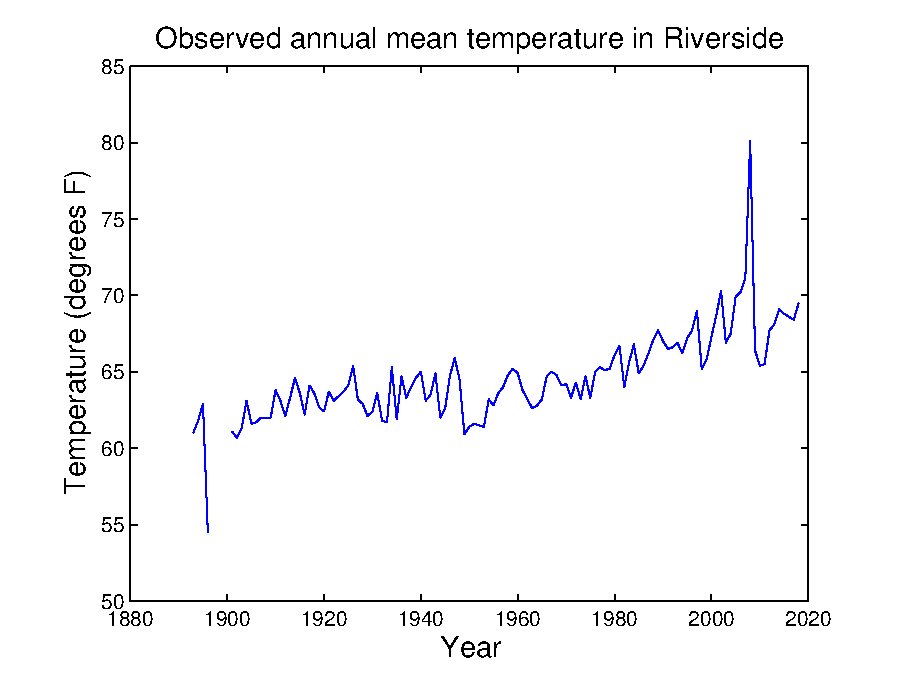
\includegraphics[width=\linewidth]{ch1-plot-temperature4.eps}
\caption{Observed annual mean surface temperature in Riverside.}
\label{fig:ch1-plot-temperature4}
\end{marginfigure}

Recall that the original global temperature data was given as an \uline{anomaly} compared to the average over some baseline (or reference) period -- in this case, year 1910 to 2000. If we treated both data sets the same, and transformed the Riverside temperature data into a comparable \uline{anomaly}, a more direct comparison could be made. 

To create an anomaly of the Riverside temperature data, relative to the mean of the data for years 1910 to 2000, requires that we know what the mean of the data is over the years 1910 to 2000. Using the \textbf{MATLAB} function \texttt{mean}, you should be able to work out that you need:
\begin{docspec}
>> tdata\_mean = mean(tdata(:,end));
\end{docspec}
and then all you need to is is to subtract that from the annual data, e.g.
\begin{docspec}
>> mean(tdata(:,end)) = mean(tdata(:,end))-tdata\_mean;
\end{docspec}
(which is talking the last column of the array, subtracting \texttt{tdata\_mean} from all the values, and writing that vector back to the last column. EXCEPT, the answer is apparently ...
\begin{docspec}
>> tdata\_mean = mean(tdata(:,end))\\
tdata\_mean = \\
NaN
\end{docspec}
\texttt{NaN}??? Oh no ...

\vspace{1mm}
Actually, more recent versions of MATLAB allow you to ignore \texttt{NaN}s in basic stats functions such as \texttt{mean}. For example, referring to \textbf{MATLAB} \texttt{help} and re-trying the example above:
\begin{docspec}
>> tdata\_mean = mean(tdata(:,end),'omitnan');
\end{docspec}
tells \textbf{MATLAB} to calculate the mean while ignoring any \texttt{NaN}s in the \textit{vector}.

\newpage 

\vspace{1mm}
\noindent\rule{4cm}{0.5pt}
\vspace{2mm}

\noindent It was mentioned earlier that there were potential 'artifacts' in the Riverside mean annual temperature data. If you view the loaded in data array in the \textsf{Variable viewing window} (double-click on the \textsf{temperature\_riverside} variable name in the \textsf{Workspace window}), you can see for a number of years and months, rather than numbers, '\texttt{NaN}'s in the cells. \texttt{NaN} stands for 'Not a Number' and indicates that there is no (valid) numerical value for that array position (cell). The impact of there being a number of months of data missing, is that the annual mean is no longer a true annual mean but rather simply the mean of whatever monthly data exists for any particular year. For example, year 2008 has no data other than during the summer and the annual mean is hence simply equal to the July temperatures!

\begin{marginfigure}[-2.25in]
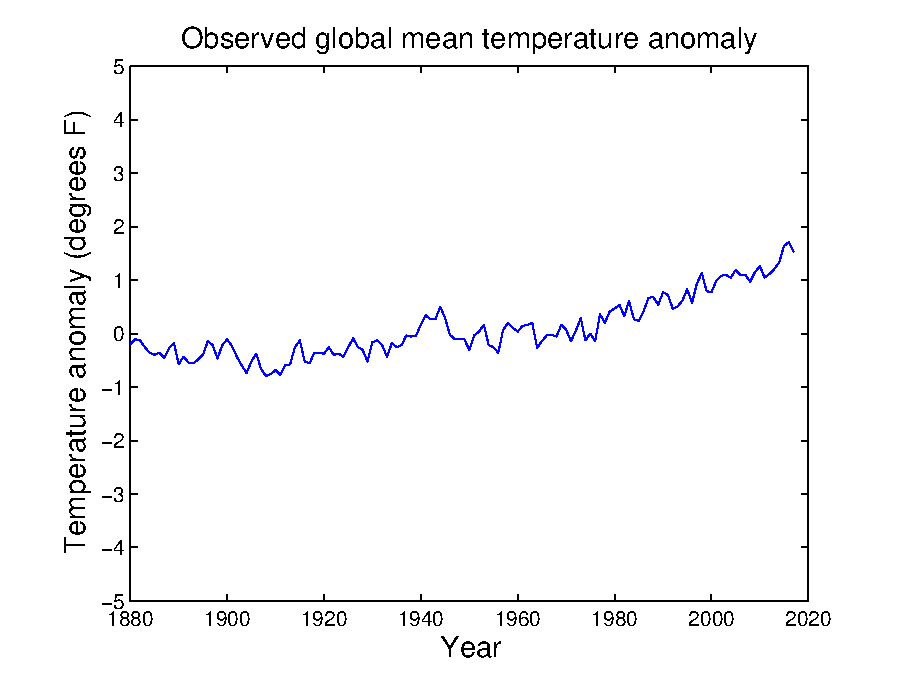
\includegraphics[width=\linewidth]{ch1-plot-temperature5.eps}
\caption{Observed global annual mean surface temperature anomaly, relative to the mean of 1910 through 2000.}
\label{fig:ch1-plot-temperature5}
\end{marginfigure}

\begin{marginfigure}[0.0in]
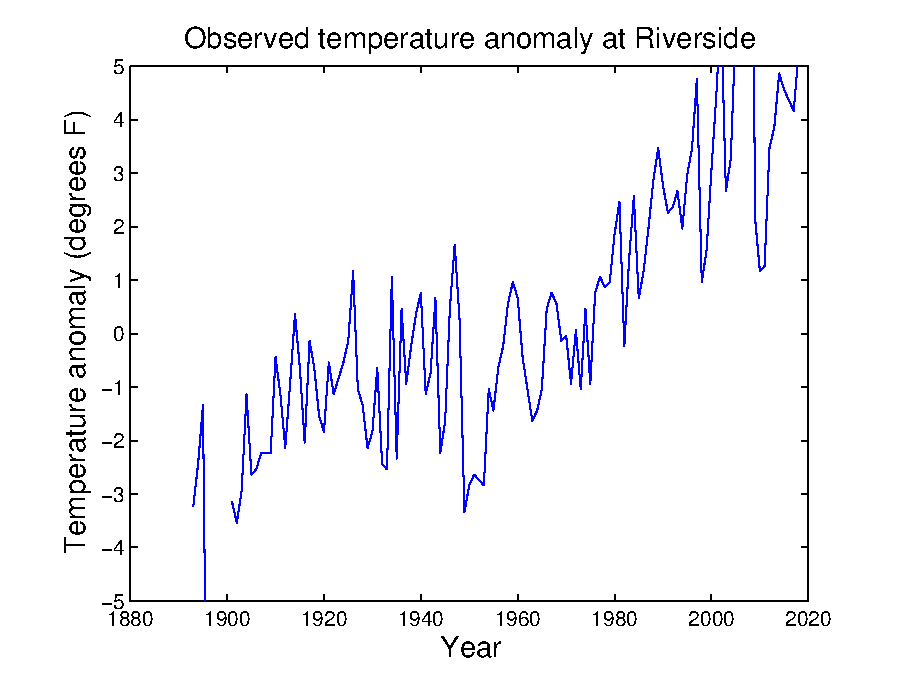
\includegraphics[width=\linewidth]{ch1-plot-temperature6.eps}
\caption{Observed annual mean surface temperature anomaly, relative to the mean of 1910 through 2000, at Riverside.}
\label{fig:ch1-plot-temperature6}
\end{marginfigure}

\begin{marginfigure}[0.0in]
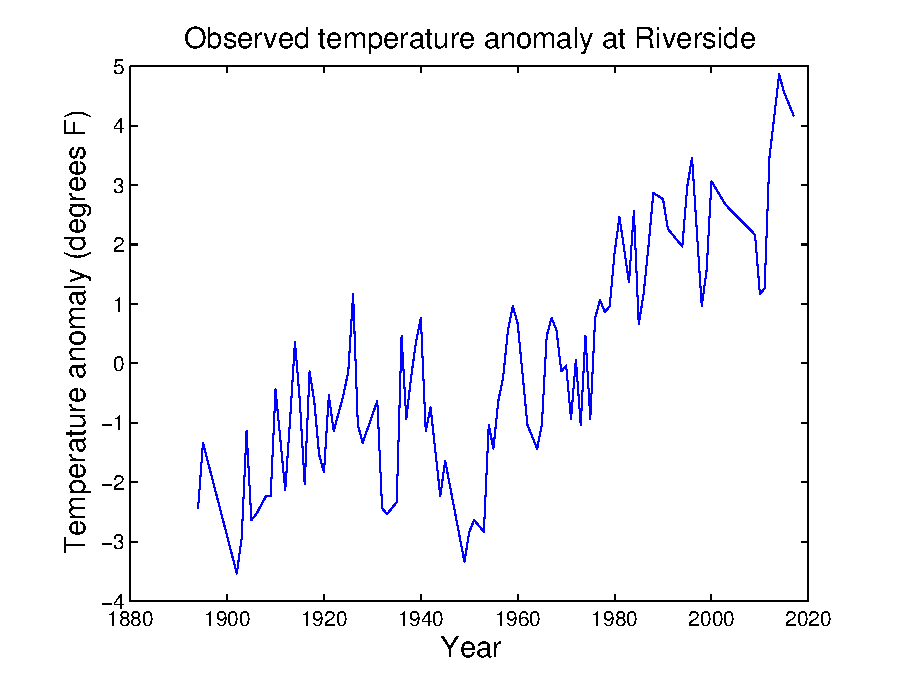
\includegraphics[width=\linewidth]{ch1-plot-temperature7.eps}
\caption{Observed annual mean surface temperature anomaly, relative to the mean of 1910 through 2000, at Riverside, filtered to remove years with missing monthly data.}
\label{fig:ch1-plot-temperature7}
\end{marginfigure}

One could address this by removing the years with (substantially) incomplete monthly data from the data file\sidenote{i.e. simply deleting the line in the file.} and prior to loading into \textbf{MATLAB}. Or would could process the data once in \textbf{MATLAB}. This can be done by assigning to particular row (vector) of data, an empty vector (\texttt{[]}). 

Taking first a simple example of a column vector:

\vspace{2mm}
\(A=\begin{pmatrix}1 \\
2 \\
3 \\
\end{pmatrix}\)
\vspace{2mm}

\noindent from which we wish to remove the 2nd row. In \textbf{MATLAB} we would create the vector by:
\begin{docspec}
>> A = [1; 2; 3];
\end{docspec}
and then remove the 2nd row by setting it to an empty element:
\begin{docspec}
>> A(2) = [];
\end{docspec}

Similarly, to remove the 2nd row of:

\vspace{2mm}
\(B=\begin{pmatrix}1 & 4 \\
2 & 5 \\
3 & 6 \\
\end{pmatrix}\)
\vspace{2mm}

\noindent we could type:
\begin{docspec}
>> B = [1, 4; 2, 5; 3, 6];\\
>> B(2,:) = [];
\end{docspec}

\noindent (instead removing e.g. the 1st column would be \texttt{B(:,1) = []})

So back to the temperature data -- to remove the row containing the year 2008 data for example\sidenote[][-0.0in]{You can also delete rows (and columns) if you open up the \textbf{MATLAB} \texttt{Array window} (double-click on the variable name in the \texttt{Workspace window}). And ... edit/replace values ...}, which is row 11, we would write:
\begin{docspec}
>> temperature\_riverside(11,:)=[];
\end{docspec}

Play this 'game' -- deleting as many row as you think result in biased means (because of missing monthly data)\sidenote[][-0.0in]{(being aware that as you delete rows, the numbering of the subsequent rows changes as the array size shrinks ...)}, with the Riverside temperature data, and re-plot the results.
For example, the result of removing ALL the rows with missing monthly data\sidenote{(There are simple and quick ways of doing this in \textbf{MATLAB} that we will see later.)}, results in Figure \ref{fig:ch1-plot-temperature7}.

\vspace{1mm}
\noindent\rule{4cm}{0.5pt}
\vspace{2mm}

\noindent Finally, go back to the original global mean anomaly values (re-load the data set if necessary) and convert from the anomaly in \degree C to \degree F (i.e. simply multiply by \(1.8\) -- no offset (32\degree F) is required in this particular case). If you additionally, chose and set a sensible common y-axis scale for both plots, you might end up with a pair of graphs looking like Figures \ref{fig:ch1-plot-temperature5} and \ref{fig:ch1-plot-temperature6}.
\sidenote[][-0.0in]{There are all sorts of likely reasons for the differences. Firstly, the global mean surface temperature rise includes both ocean surface and land surface. Because of the higher heat capacity of the ocean, the ocean surface warms slower than the land, and the ocean accounts for ca. 70\% of the total global surface area. So it is somewhat inevitable that the warming trend will be stronger in Riverside. It may also be that the Riverside data is influenced by the 'urban heat island' effect, in which long0-term measured trends can be affected by increasing urbanization of the area surrounding the weather station. It may also be that the latitude and specific location of Riverside, sees much more warming that the global mean.}

%------------------------------------------------

\newpage

%------------------------------------------------

\section{Even nicer graphing and graphics}

There are a bunch of simple \textbf{MATLAB} drawing and text placement commands that can help improve the look and feel of scientific plots, or even replace the provided plotting functions (i.e. you can create your own bespoke plotting functions). There are also a variety of options for altering the axes, axes tick-marks, axes tick-mark labels, etc that can be useful.

%------------------------------------------------

\newpage

%------------------------------------------------

\subsection{Drawing lines (and using handles)}

\marginnote[-0.125in]{\begin{mdframed}[backgroundcolor=gray!10, roundcorner=10pt,leftmargin=1, rightmargin=1, innerleftmargin=5, innerrightmargin=5, innertopmargin=5,innerbottommargin=5, outerlinewidth=1, linecolor=light-gray]
\docenvdef{line}
\\To draw a simple (single) line on a graphic:
\begin{docspecmargin}
>> line ... \\([x1 x2],[y1 y2])
\end{docspecmargin}
where \texttt{x1} and \texttt{x2} are the \textit{x}-coordinates of the start and end position of the line, and \texttt{y1} and \texttt{y2} are the corresponding \textit{y}-coordinate values.
\\You can also specify line colors and styles in a similar way to when using \texttt{plot}, e.g.
\begin{docspecmargin}
>> line ... \\([x1 x2],[y1 y2], ... 'Color','red', ... 'LineStyle','--')
\end{docspecmargin}
plots a red dashed line.
\end{mdframed}}

We'll start with some simple line  drawing. 

At the command line -- open a new \textsf{figure window} (\texttt{>> figure;}). Then before anything else, do a \texttt{>> hold on;}.

When \textbf{MATLAB} draws lines and shapes and places text, it needs to know the coordinates of where to place things. It is not possible (I think) to draw directly in the \textsf{figure window} -- \textbf{MATLAB} needs what is known as a \textit{frame} to put things in, and the easiest way to do this is to create a set of axes. Having opened a new \textsf{figure window} (even through you have not plotted any data!), set the x- and y-axis range\sidenote{Here taking the example range of 0-100 on both axes.}:
\begin{docspecbold}
>> axis([0 100 0 100]);
\end{docspecbold}
The resulting figure is really not very exciting (Figure \ref{fig:ch3-graphics01}).

\begin{marginfigure}[0.0in]
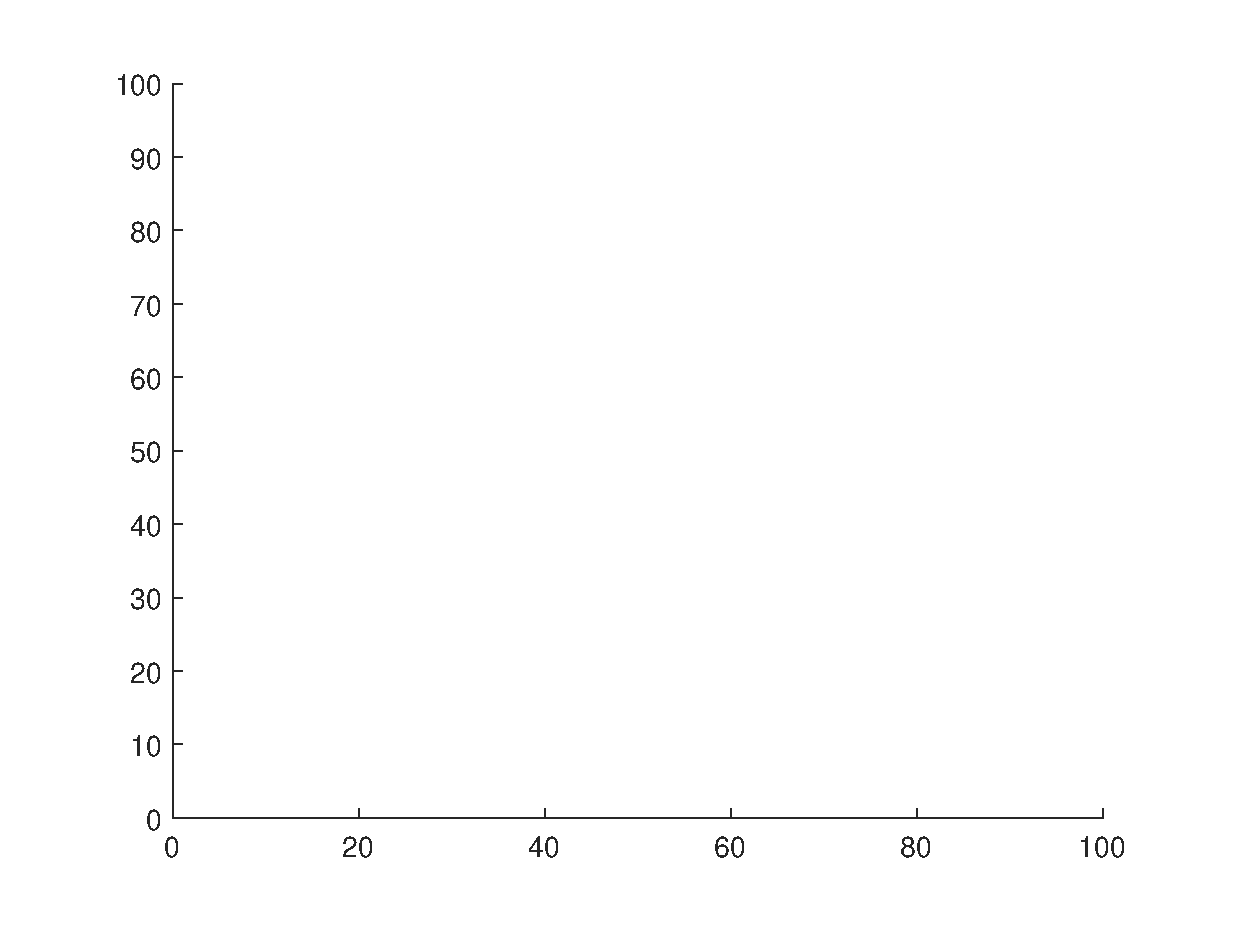
\includegraphics[width=\linewidth]{ch3-graphics01.eps}
\caption{Figure window with axes.}
\label{fig:ch3-graphics01}
\end{marginfigure}

\begin{marginfigure}[-0.0in]
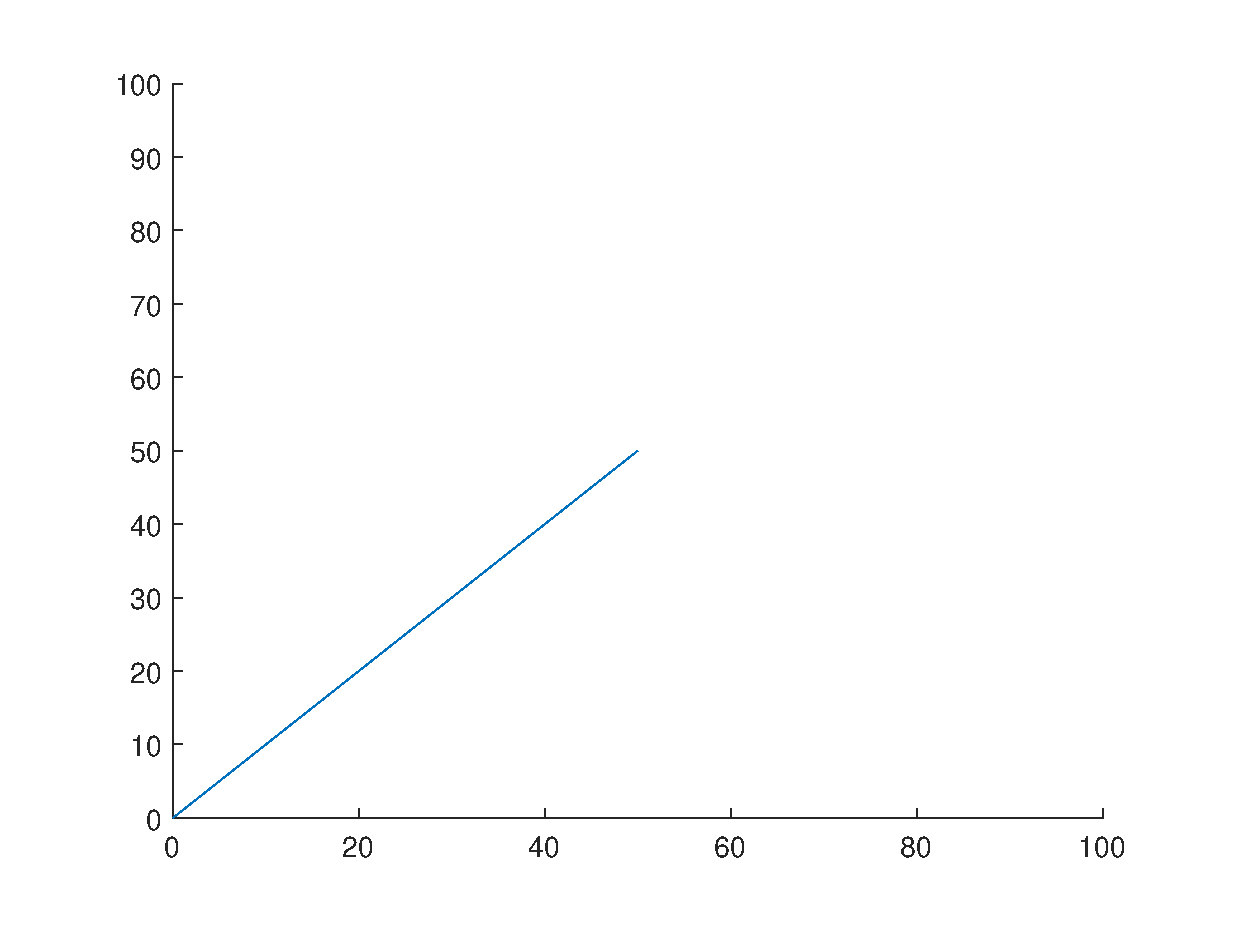
\includegraphics[width=\linewidth]{ch3-graphics02.eps}
\caption{Figure window with single line segment (via \texttt{plot}).}
\label{fig:ch3-graphics02}
\end{marginfigure}

\begin{marginfigure}[-0.0in]
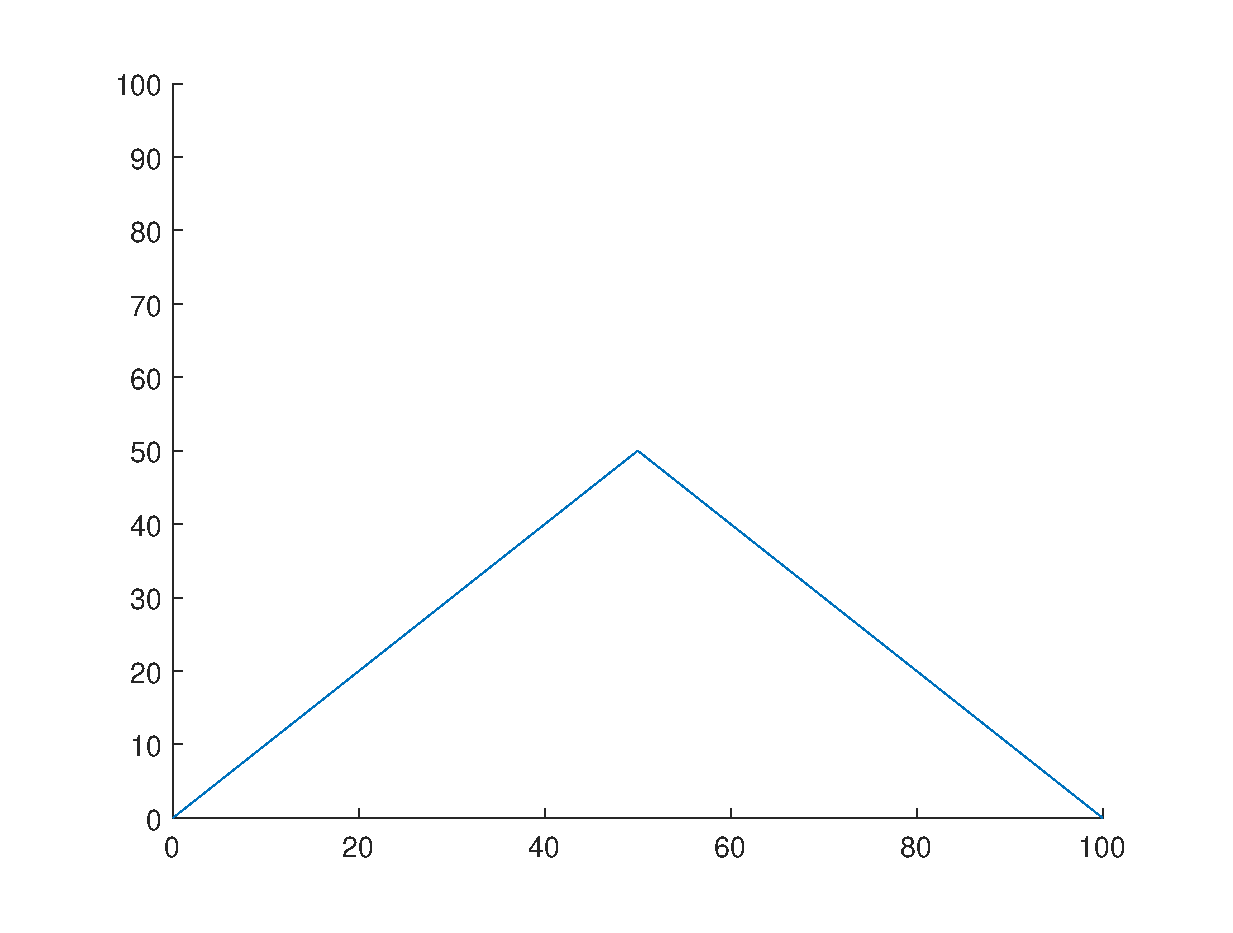
\includegraphics[width=\linewidth]{ch3-graphics03.eps}
\caption{Figure window with a second line segment (via \texttt{line}).}
\label{fig:ch3-graphics03}
\end{marginfigure}

\vspace{1mm}
\noindent\rule{4cm}{0.5pt}
\vspace{2mm}

\noindent There are 2 ways to draw a line (examples assuming the previous Figure window remains open with \texttt{hold on} ...):

\vspace{-2mm}
\begin{enumerate}[noitemsep]

\item \texttt{plot}
\\Are you recall, \texttt{plot} will plot a sequence of (x,y) points, and by default, join the points up with a line. If we wanted a diagonal line, from the origin to the mid-point of the plot area, we could invent a pair of vectors to define the two points we need -- at (0,0) and (50,50):
\begin{docspecbold}
X1 = [0 50];\\
Y1 = [0 50];
\end{docspecbold}
and then plot the resulting points as a \texttt{plot} plot:
\begin{docspecbold}
plot(X1,Y1);
\end{docspecbold}
You should now see something like Figure \ref{fig:ch3-graphics02}. (If you find that the plot area has been re-sized such that the x- and y-axes now both go from 0-50, then you have forgotten to do a \texttt{hold on}.)

\vspace{1mm}
\item \texttt{line}
\\ \noindent \textbf{MATLAB} provides a specific command for drawing lines ... \docenv{line}. In its simplest usage, it is a little like \texttt{plot}, except taking only a single pair of x- and y-coordinate values.
\\To use \texttt{line} to draw a 2nd line segment, starting at (50,50) and terminating at (100,0), we create another pair of vectors to define these points:
\begin{docspec}
X2 = [50 100];\\
Y2 = [50 0];
\end{docspec}
and then draw it:
\begin{docspec}
line(X2,Y2);
\end{docspec}
as shown in Figure \ref{fig:ch3-graphics03}.
\end{enumerate}

\noindent Obviously, both line segments could equally well be drawn using \texttt{plot} or \texttt{line}.

\vspace{1mm}
\noindent\rule{4cm}{0.5pt}
\vspace{2mm}

\noindent If you are just drawing, rather than annotating a plot with axes, then you might want to turn off, or hide, the axes tick marks and tick labels. To do this, we first need to find the special \textbf{MATLAB} ID of the axes, which helpfully, because you only have one set of axes and have just been using them, is the 'current axis'. To do this, we use the \docenvdef{gca} function, which returns the \textit{handle} (ID) of the axes:
\begin{docspecbold}
>> h = gca;
\end{docspecbold}

\noindent Having got the axis \textit{handle}\sidenote[][2.0in]{It is worth omitting the \texttt{;} in order to see the properties associated with the axes, and in fact, it is worth clicking on \texttt{Show \uline{\textcolor{blue}{all properties}}} to see a list of everything that can be edited and adjusted. \\ALL these can be changed if you ever want!!!}, we can now 'set' the properties of the axes, using \docenvdef{set}:
\begin{docspecbold}
>> set(h,'XTick',[],'XTickLabel','');
\end{docspecbold}

What this does is to tell \textbf{MATLAB}: take the graphics object with the ID contained in variable \texttt{h} (which we just retried via the \texttt{gca} function), and set (which is why we use the command \texttt{set} ...) the following properties:
\begin{itemize}[noitemsep]
\setlength{\itemindent}{.2in}
\item \texttt{'XTick',[]} -- set the number and position of tick marks on the x-axis, to the contents of the empty vector \texttt{[]}.
\item \texttt{'XTickLabel',''} -- set the labels applied to the tick-marks, to \texttt{''} (i.e. no text).
\end{itemize}

\noindent Actually, in this example, the 2nd graphics parameter set (the labels) is sort of redundant, as there are no tick-marks in the first place ... 

To see how different combinations of settings pan out, try:
\begin{docspecbold}
>> set(h,'XTick',[0 50 100],'XTickLabel','');
\end{docspecbold}
(3 small inwards ticks, no labels)
\begin{docspecbold}
>> set(h,'XTick',[0 50 100],'XTickLabel','cat');
\end{docspecbold}
:o)
\\\noindent and/or:
\begin{docspecbold}
>> set(h,'XTick',[0 50 100],'XTickLabel',\{'cat', 'dog', 'rabbit'\});
\end{docspecbold}
where \texttt{\{'cat', 'dog', 'rabbit'\}} is actually a 3 string \textit{cell array} (the curly brackets are \uline{important} to the syntax).

All this insanity should be looking like Figure \ref{fig:ch3-graphics04} (if we also remove the y-axis ticks and labels\sidenote[][-1.5in]{It is sufficient just to type: \begin{docspecmargin}>> set(h,'YTick',[]);
\end{docspecmargin}}).

\begin{marginfigure}[-1.0in]
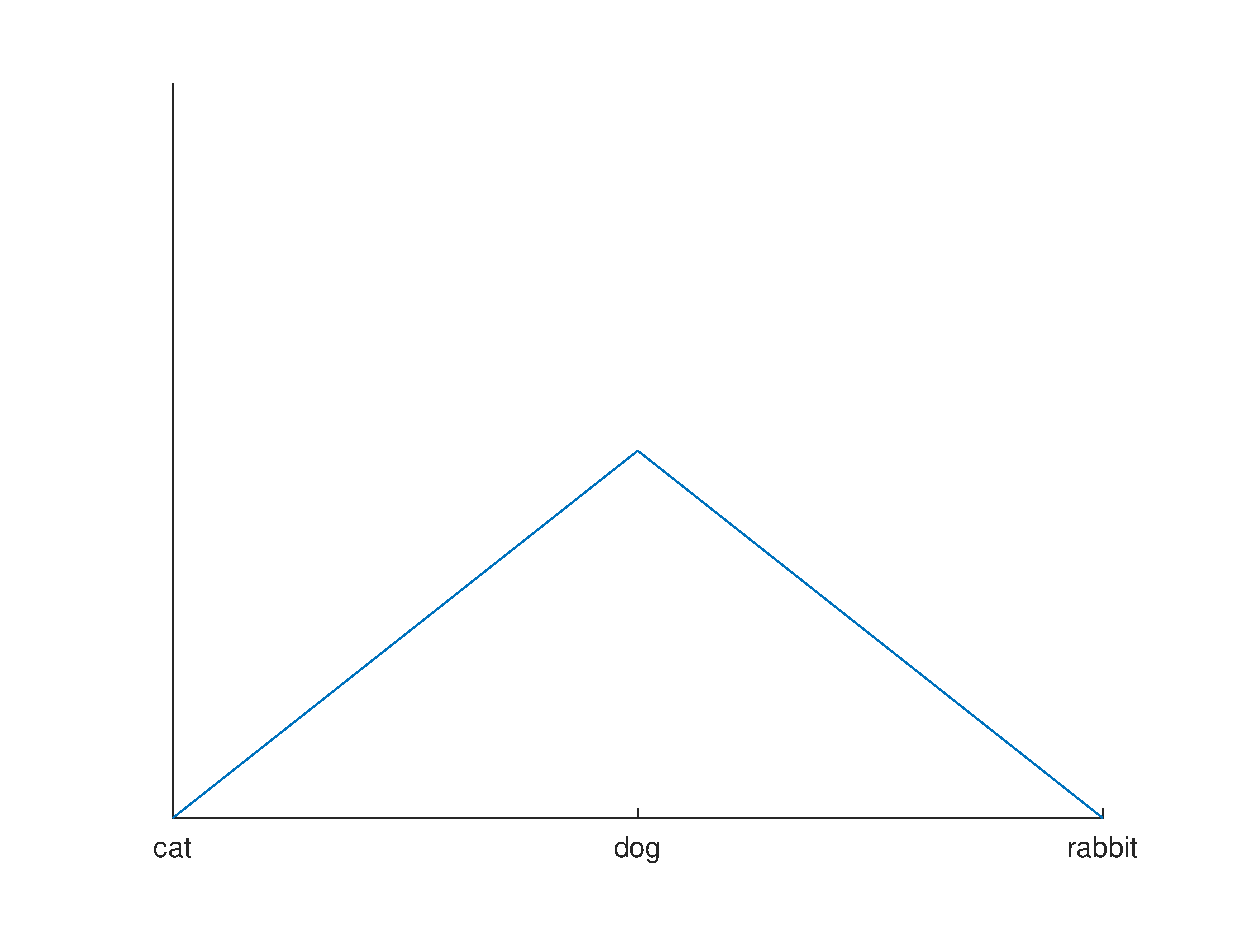
\includegraphics[width=\linewidth]{ch3-graphics04.eps}
\caption{(no comment).}
\label{fig:ch3-graphics04}
\end{marginfigure}

\vspace{1mm}
\noindent\rule{4cm}{0.5pt}
\vspace{2mm}

\newpage

\noindent An alternative way to create a figure to draw on, without having to remove the axes ticks and labels etc etc, is to create the axes as 'invisible' in the first place. To try this -- first create a new \textsf{figure window}.\sidenote{If you find yourself drowning in \textsf{figure window}s, remember that \texttt{close} closes the current window, and \texttt{close all} closes all of them.}
\begin{docspecbold}
>> h = axes('Position',[0 0 1 1],'Visible','off');
\end{docspecbold}
Here, \texttt{'Position',[0 0 1 1]} specifies that the axes area should fill the window, and \texttt{'Visible','off'} says to make the axes invisible. (We keep a copy of the \textit{handle} variable, \texttt{h}, just in case we need it later.) And to set the axes to the same 0-100 limits as before:
\begin{docspecbold}
>> axis([0 100 0 100]);
\end{docspecbold}
Then \texttt{hold on} to start drawing things!\footnote{For some reason ... you need to do \texttt{hold on} only \uline{after} creating axes frame ...}

Try drawing some lines in this window (remembering the 0-100 axes limits when making up (x,y) co-ordinates).

\vspace{1mm}
\noindent\rule{4cm}{0.5pt}
\vspace{2mm}

\noindent The command \docenv{set} can be used in the context of any (I think?) graphics object, i.e. any individual component part of a final plot such as the axis line itself, the axis ticks, plotted lines and points, etc. For example, in creating the line segment previously:
\begin{docspecbold}
>> h = line(X2,Y2);
\end{docspecbold}
you could store a copy of the \textit{handle} of that line segment -- here it is being assigned to the \textit{variable} \texttt{h}. With this, you can now change the properties of the line (after you have drawn it). such as by:
\begin{itemize}[noitemsep]
\setlength{\itemindent}{.2in}
\item \textbf{\texttt{>> set(h,'LineWidth',2.0);}}
\\will change the line width to 2.0 (points). 
\item \textbf{\texttt{>> set(h,'Color',[1 0 0]);}}
\\will turn the line red, using the \textit{RGB} (red-green-blue) notation: \\\texttt{[1 0 0]}\sidenote{Alternatively:
\begin{docspecmargin}set(h,'Color','r');
\end{docspecmargin}}.
\item \textbf{\texttt{>> set(h,'LineStyle',':');}}
\\\noindent will make the line dotted. 
\end{itemize}

\noindent Note that here, you are setting line properties \uline{after} you have created the graphics, whereas earlier in eg. using \texttt{plot} to graph data, you specified the properties at the same time as you draw the lines. Both ways are valid, but being able to change properties later and after plotting, gives you greater flexibility. Note that after plotting a graphic, you can also edit and adjust its properties in the \textsf{Figure window} itself (via its GUI)

\vspace{1mm}
\noindent\rule{4cm}{0.5pt}
\vspace{2mm}

\noindent Using a \textit{handle} also now enables you to complete an earlier plot. For the proxy \(CO_{2}\) data where you color-coded the points and added a \texttt{colorbar}, there was not actually any indication of what the color scale actually means in terms of values (and of what). \textbf{MATLAB} will add a colorbar to a plot with the command ... \docenv{colorbar}. Although the color scale gets automatically plotted with labels for the values, looking at the plot, we still don't know what the values are of (e.g. units). We can label the colorbar, but \textbf{MATLAB} needs to know what we are labelling. Each graphic object is assigned a unique ID when you create them and which normally you know nothing about. We can create a variable to store the ID, and then pass this ID to \textbf{MATLAB} to tell it to create a title for the colorbar. To cut a long story short, you would add to your \textit{script} file:
\begin{docspec}
colorbar\_id=colorbar;
\\title(colorbar\_id,'Relative error (\%)';
\end{docspec}
The revised plot should then end up looking something like Figure \ref{fig:plot-CO2scatter4} in which you can see the high relative uncertainty (bight colors) prevail at low CO\(_{2}\) values and 'deeper time' (ca. 200-300 Ma). The colorbar title (label) is maybe not ideal, nicer would be one aligned vertically rather than horizontally. We'll worry about that sort of refinement another time.

\begin{marginfigure}[-0.0in]
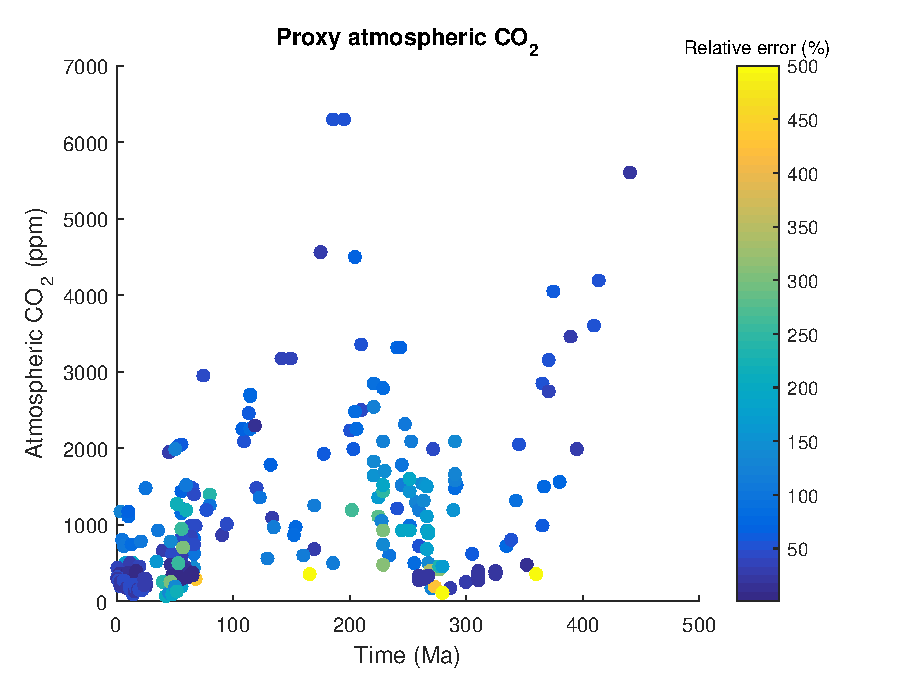
\includegraphics[width=\linewidth]{plot-CO2scatter4.eps}
\caption{Proxy reconstructed past variability in atmospheric CO2 (scatter plot).}
\label{fig:plot-CO2scatter4}
\end{marginfigure} 



\vspace{1mm}
\noindent\rule{4cm}{0.5pt}
\vspace{2mm}

\noindent An obvious use for drawing lines on plots, is to annotate them. e.g. placing a text label (we'll see shortly), with a line pointing from the text to a specific feature. You can do with with a simple line and hence the \texttt{line} command.

It would be more handy and in fact common, to include an arrow head to make clear that the line is pointing to something. This can in theory be done by drawing 2 more, shorter lines, but is no fun at all\sidenote{True fact -- I have tried it :(}. \textbf{MATLAB} hence provides the function \docenvdef{quiver}. \texttt{quiver} is commonly used for plotting fields of arrows, but can equally be used to create a single arrow -- much like earlier you used \texttt{plot} to draw just a single pair of joined up points and hence a line. However, rather than take a pair of (x,y) points -- one for the start and one for the end, of the line, \texttt{quiver} takes an (x,y) location for the start of the arrow, and then the \uline{length} in the x and y directions.

Consistent with the previous example, we were starting the line segment at (0,0), and then extending the line to (50,50). The length vector in this case is also [50 50]. So, given the specific syntax and input parameter format required by \textbf{MATLAB} for this function\sidenote{Here -- the last, 5th parameter (\texttt{0}), tells \textbf{MATLAB} not to auto-scale the arrow.}\sidenote{If your arrow head is hard to make out -- try creating a new \textsf{figure window}. You can also use \texttt{cls} to clear all the graphics in the window (i.e. and not have to re-generate the \textsf{figure window}.}:
\begin{docspecbold}
>> quiver(0,0,50,50,0);
\end{docspecbold}

To make the syntax clearer and that we are passing 4 vectors (of x and y origin locations, and x- and y-axis lengths), we could also write:
\begin{docspecbold}
>> quiver([0],[0],[50],[50],0);
\end{docspecbold}

%------------------------------------------------

\subsection{Colors}

You are already familiar with setting colors for lines, with the notation: \texttt{'r'}, or \texttt{'b'} (for red, blue, respectively). This is nice and simple and so totally fabulous ... except there are a limited number of colors available in this notation (see Box).

\marginnote[-0.875in]{\begin{mdframed}[backgroundcolor=gray!10, roundcorner=10pt,leftmargin=1, rightmargin=1, innerleftmargin=5, innerrightmargin=5, innertopmargin=5,innerbottommargin=5, outerlinewidth=1, linecolor=light-gray]
\textbf{MATLAB} quick colors:
\begin{itemize}[noitemsep]
\setlength{\itemindent}{.2in}
\item \texttt{y} -- yellow
\item \texttt{m} -- magenta
\item \texttt{c} -- cyan
\item \texttt{r} -- red
\item \texttt{g} -- green
\item \texttt{b} -- blue
\item \texttt{w} -- white
\item \texttt{k} -- black
\end{itemize}
\end{mdframed}}

Hence there is an alternative that enables a more exact specification of color. In this particular scheme -- red-green-blue, abbreviated to \textit{RGB}, you set the intensity of red, green, and blue, on a scale of 0 to 1. And supply this in a vector format to \textbf{MATLAB}. For example:

\begin{marginfigure}[-0.0in]
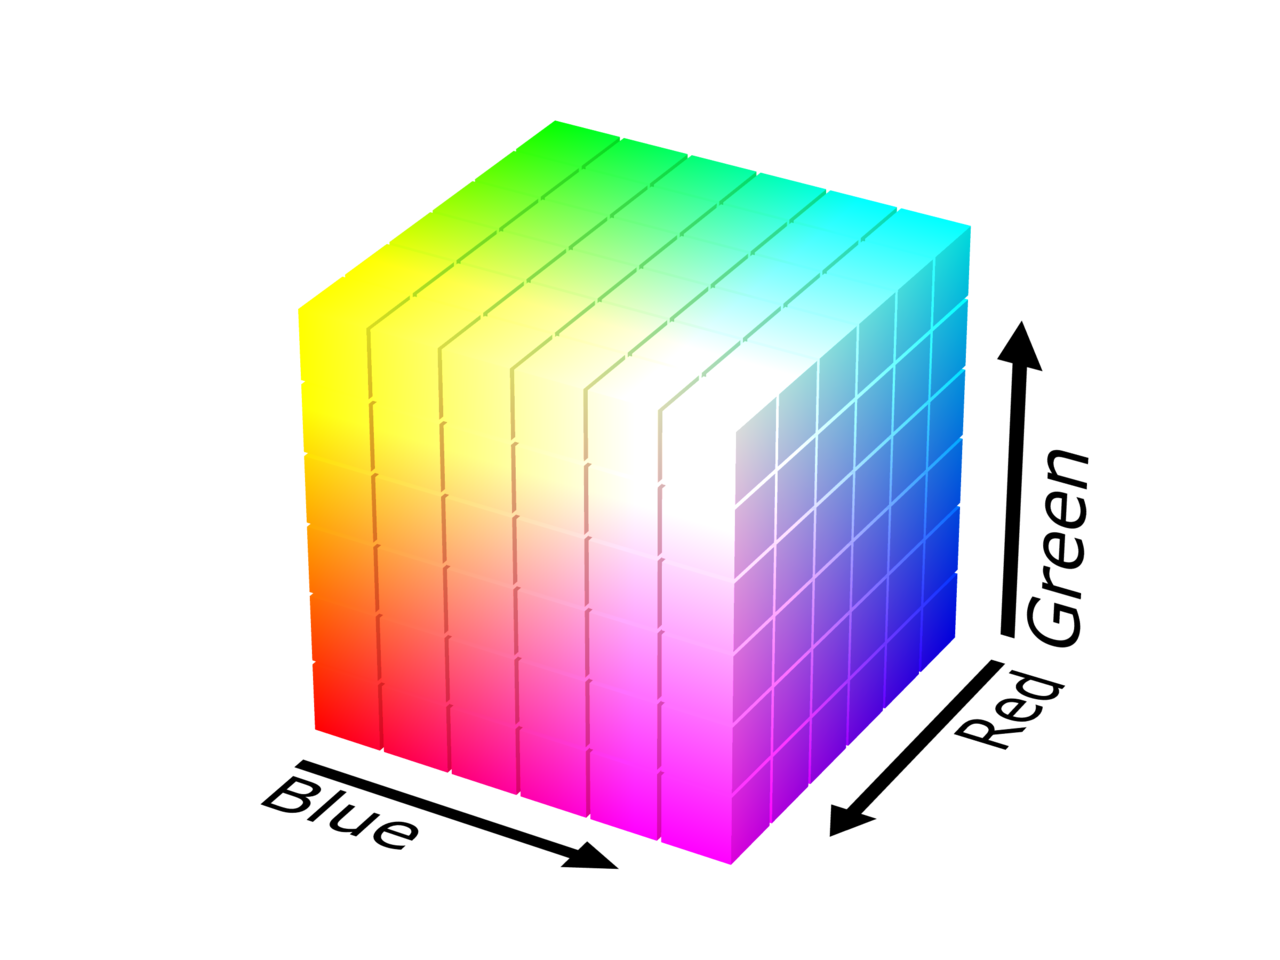
\includegraphics[width=\linewidth]{RGB_color_solid_cube.png}
\caption{RGB scale. By SharkD - Own work, GFDL, https://commons.wikimedia.org/
w/index.php?curid=3375025}
\label{fig:RGB_color_solid_cube}
\end{marginfigure}

\begin{itemize}[noitemsep]
\setlength{\itemindent}{.2in}
\item \texttt{[0 0 0]} -- zero intensity of all of R, G, B => black.
\item \texttt{[1 1 1]} -- 100\% intensity of all of R, G, B => white.
\item \texttt{[1 0 0]} -- 100\% intensity R, none for G and B => red.
\item \texttt{[0.5 0.5 0.5]} -- 50\% intensity of all of R, G, B => grey.
\item \texttt{[0.5 1.0 0.5]} -- light green.
\end{itemize}

Play around with some RGB value combinations, plotting shapes, or filled circles, e.g.
\begin{docspecbold}
>> scatter(50,50,1000,[0.25 0.75 0.25],'filled');
\end{docspecbold}

A rendition of the RGB color scale is shown for reference in Figure \ref{fig:RGB_color_solid_cube}. 
%------------------------------------------------

\subsection{Shapes}


\marginnote[-0.125in]{\begin{mdframed}[backgroundcolor=gray!10, roundcorner=10pt,leftmargin=1, rightmargin=1, innerleftmargin=5, innerrightmargin=5, innertopmargin=5,innerbottommargin=5, outerlinewidth=1, linecolor=light-gray]
\docenvdef{patch}
\\To plot one (or more) filled polygonal regions, pass 2 vectors of the x and y as the coordinates for each vertex, e.g.
\begin{docspecmargin}
>> patch(X,Y,C)
\end{docspecmargin}
where \texttt{X} and \texttt{Y} are the \textit{x}- and \textit{y-}coordinates of the vertices. \texttt{C} determines the polygon's color.
\\For example, a red square would be:
\begin{docspecmargin}
x = [0 1 1 0];\\
y = [0 0 1 1];\\
patch(x,y,'red')
\end{docspecmargin}
\end{mdframed}}


\noindent For 2D shapes -- you can draw polygons using the \textit{function} \docenvdef{patch}. This takes as parameter input, a vector of x-coordinate positions, then a vector of y-coordinate positions, and as a 3rd parameter, the color for the object.

So in our previous example, with the x- and y-axes going from 0-100, say we want to draw a square in the middle, 20 units on each side. We could create our vector of x-axis coordinates as such:
\begin{docspecbold}
>> X1 = [40 40 60 60];
\end{docspecbold}
and for the y-axis ... (some care is needed and often it might be helpful to sketch out the coordinate pairs and positions on a piece of paper):
\begin{docspecbold}
>> Y1 = [40 60 60 40];
\end{docspecbold}
To draw, simply pass the 2 coordinate vectors to \texttt{patch}, along with any line style specification:
\begin{docspecbold}
>> patch(X1,Y1,'r');
\end{docspecbold}
as shown in Figure \ref{fig:ch3-shape01}. 

Note that in this \texttt{(X1,Y1)} point notation, we are telling \textbf{MATLAB} to plot a shape with vertices at:

\vspace{2mm}
\((40,40), (40,60), (60,60), (60,40)\)
\vspace{2mm}

\noindent Also note that \uline{the order of the (x,y) pairs, matters}, as \textbf{MATLAB} draws the line segments between the vertices in the order that they are given to \textbf{MATLAB} (as per for \texttt{plot}). For the same (x,y) pairs, try creating \texttt{X1} and \texttt{Y1} vectors with the pairs in a different order and see what happens.

\begin{marginfigure}[-2.0in]

\includegraphics[width=\linewidth]{ch3-shape01.eps}
\caption{Square.}
\label{fig:ch3-shape01}
\end{marginfigure}

Slightly changing the values of the (x,y) pairs can also give you a diamond (-ish):
\begin{docspecbold}
>> X2 = [40 50 60 50];\\
>> Y2 = [50 60 50 40];\\
>> patch(X2,Y2,'c');
\end{docspecbold}
as shown in Figure \ref{fig:ch3-shape02}.

\begin{marginfigure}[-1.0in]
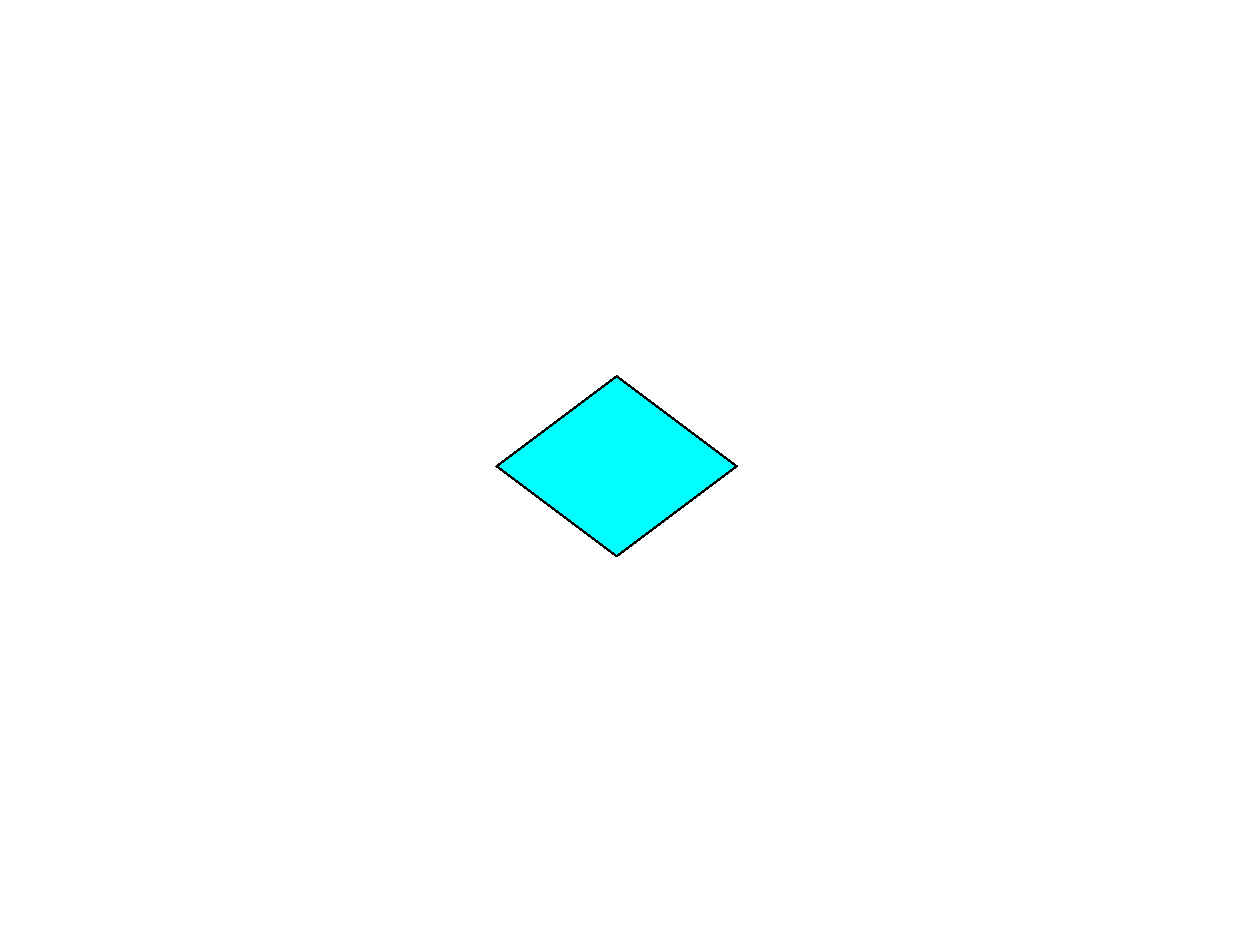
\includegraphics[width=\linewidth]{ch3-shape02.eps}
\caption{Alt square.}
\label{fig:ch3-shape02}
\end{marginfigure}

\texttt{patch} is in fact much more flexible than I have shown so far, and in fact, will draw \uline{any} polygon. Consider this sort of slightly random series of x and y coordinates: 
\begin{docspec}
>> X3 = [20 40 60 80 60 40];\\
>> Y3 = [50 60 50 60 40 30];
\end{docspec}
\begin{docspec}
>> patch(X3,Y3,'g');
\end{docspec}
gives Figure \ref{fig:ch3-shape03}.

\begin{marginfigure}[-0.0in]
\includegraphics[width=\linewidth]{ch3-shape03.eps}
\caption{Random polygon.}
\label{fig:ch3-shape03}
\end{marginfigure}

Try designing/playing about with different shapes. Perhaps sketch them out on paper first and list down the coordinates before telling \textbf{MATLAB}.

\vspace{1mm}
\noindent\rule{4cm}{0.5pt}
\vspace{2mm}

\noindent If you have the \textbf{MATLAB} \textsf{Image Processing Toolbox} installed, then you can use the command \texttt{viscircles} to draw circles.

If not -- a crude but sometimes effective alternative, is to \texttt{scatter} plot a single point ((x,y) location), and set a large size value for the circle. For example:
\begin{docspecbold}
>> scatter(50,50,1000);
\end{docspecbold}
or filled:
\begin{docspecbold}
>> scatter(50,50,1000,'filled');
\end{docspecbold}

%------------------------------------------------

\newpage
\subsection{Placing and making text 'nice'}

There is not much to placing text and specifying its properties. The \textbf{MATLAB} command for writing a string to a \textsf{figure window}, is \docenv{text}. That's it! (see Boxes)

\marginnote[-0.75in]{\begin{mdframed}[backgroundcolor=light-gray, roundcorner=10pt,leftmargin=1, rightmargin=1, innerleftmargin=5, innerrightmargin=5, innertopmargin=5,innerbottommargin=5, outerlinewidth=1, linecolor=light-gray]
\docenvdef{text}
\begin{docspecmargin}
text(X,Y,STRING);
\end{docspecmargin}
will write the string contained in the variable STRING (or you can pass the text as a string directly), at location (X,Y).
\\Note that by default, MATLAB alights the left-hand edge of the text with the X coordinate position, and the mid-point of the string vertically, with the Y coordinate. i.e. the string is \textit{left-aligned} and \textit{centered} vertically.
\\A variety of additional properties can be set at the time, e.g.
\begin{docspecmargin}
text ...
(X,Y,STRING,'FontSize',12);
\end{docspecmargin}
specifies a 12 pt font size. Other common parameter options include:
\begin{itemize}[noitemsep]
\setlength{\itemindent}{.2in}
\item \texttt{'FontName'}
\item \texttt{'Color'}
\item \texttt{'Rotation'}
\item \texttt{'HorizontalAlignment'}
\item \texttt{'VerticalAlignment'}
\end{itemize}
See \textbf{MATLAB} \texttt{help} for more details.
\end{mdframed}}

For instance, you could write:
\begin{docspecbold}
>> text(25,25,'bananas');
\end{docspecbold}
\noindent and the text \texttt{bananas} will appear at location \((25,25)\) on your plot.

Additional parameters can be added to change font, size, etc (see Box), e.g.:
\begin{docspecbold}
>> text(25,25,'bananas','FontSize',24,'Color',[0 1 1]);
\end{docspecbold}

\noindent for big light blue 'bananas'.

\marginnote{\begin{mdframed}[backgroundcolor=light-gray, roundcorner=10pt,leftmargin=1, rightmargin=1, innerleftmargin=5, innerrightmargin=5, innertopmargin=5,innerbottommargin=5, outerlinewidth=1, linecolor=light-gray]
When \textbf{MATLAB} displays text, be aware that there are a bunch of special characters that may not come out as the character you want. The more common ones are:
\\ \texttt{\_} -- will make the following character a subscript, or a sequence of characters if you place them within a pair of curly brackets \{\}.
\\ \texttt{\(\wedge\)} -- will make the following character a subscript, or a sequence of characters if you place them within a pair of curly brackets \{\}.
\end{mdframed}}

%------------------------------------------------
%
\newpage

\subsection{Creating color maps}

\marginnote[-0.25in]{\begin{mdframed}[backgroundcolor=gray!10, roundcorner=10pt,leftmargin=1, rightmargin=1, innerleftmargin=5, innerrightmargin=5, innertopmargin=5,innerbottommargin=5, outerlinewidth=1, linecolor=light-gray]
\docenvdef{colormap} (2)
\\ As mentioned earlier, \textbf{MATLAB} has a number of 'colormaps' built in, which are:

\begin{itemize}[noitemsep]
\item parula (default)
\item jet (old default ... avoid ...!)
\item hsv
\item hot    
\item cool
\item spring
\item summer
\item autumn
\item winter
\item gray
\item bone
\item copper
\item pink
\item lines
\item colorcube
\item prism
\item flag
\end{itemize}

\noindent and which you can set by:
\begin{docspecmargin}
>> colormap NAME
\end{docspecmargin}
\noindent (or \texttt{colormap(NAME)}), e.g.:
\begin{docspecmargin}
>> colormap 'hot'
\end{docspecmargin}
\noindent (or \texttt{colormap('hot')})

\end{mdframed}}

As mentioned earlier -- \textbf{MATLAB} enables a range of different color scales (\textit{colormaps}) to be used in (esp. contour) plotting and provides around  dozen built-in possibilities (see Box).

Taking the earlier example of loading and plotting the global topography data:

\begin{docspec}
>> data = load('etopo1deg.dat','-ascii');\\
>> imagesc(data);
\end{docspec}

\noindent gives Figure \ref{fig:ch3-etopo3}, and

\begin{docspec}
>> colormap('hot');\\
>> imagesc(data);
\end{docspec}

\noindent gives Figure \ref{fig:ch3-etopo3}.

\begin{marginfigure}[0.0in]
\includegraphics[width=\linewidth]{ch3-etopo3.eps}
\caption{Global topography plotted with the default \textbf{MALTAB} color scheme.}
\label{fig:ch3-etopo3}
\end{marginfigure}

You can also define your own \textit{colormap}. \textit{Colormaps} are simply a matrix of \([R G B]\) colors. The most trivial \textit{colormap} would be:

\begin{docspec}
>> cmap1 = [0 0 0];\\
>> colormap(cmap1);
\end{docspec}

\noindent creates and applies a \textit{colormap} containing a single color (black). Try it ... but ti is clearly not very useful ...

Better, would be:

\begin{docspec}
>> cmap2 = [0 0 0; 1 1 1];\\
>> colormap(cmap2);
\end{docspec}

\noindent which creates and applies a color scale containing 2 colors - black and white and when used for the topography data, gives Figure \ref{fig:ch3-etopo5}. 
\sidenote{Remember, \texttt{imagesc} plots using the maximum number of colors available, and in this example, the mid value between the deepest place in the ocean and highest point on land, divides the colors into black and white -- within specifying a particular scale, this color separation does not occur at zero (sealevel)}

You can keep adding colors, e.g.

\begin{docspec}
>> cmap3 = [0 0 0; 0.5 0.5 0.0; 0.0 0.5 0.5; 1 1 1];
\end{docspec}

\noindent but this is a lot of effort to keep adding single additional colors. What you really want to do, is to define end-member colors, and then tell \textbf{MATLAB} to \textit{interpolate} in between these. Recalling back a couple of subsections:

\begin{docspec}
>> ynew = interp1(xold,yold,xnew);
\end{docspec}

\noindent takes the y-values (\texttt{yold}) at x-values \texttt{xold}, and interpolates onto the x-values   defined by the vector \texttt{xnew} (and assigns the new y-values to vector \texttt{ynew}). For instance, if we have the following crudely spaced data\sidenote{In MATLAB notation:
\begin{docspecmargin}
xold = [0 3 7 13 16 22 30];\\
yold = [0.2 0.6 0.7 0.3 0.3 0.1 0.0];
\end{docspecmargin}
}:

\vspace{2mm}
\(\begin{pmatrix}
0 & 0.2 \\
3 & 0.6 \\
7 & 0.7 \\
13 & 0.3 \\
16 & 0.3 \\
22 & 0.1 \\
30 & 0.0 \\
\end{pmatrix}\)
\vspace{2mm}

\noindent and we wanted to create an interpolated dataset from \(0.0\) to \(30.0\) (in x-axis values) in steps of \(1.0\), we would first create the new x-axis vector that the data will be interpolated on to:

\begin{docspec}
xnew = [0.0:1.0:30.0];
\end{docspec}

\noindent and then we would write:

\begin{docspec}
>> ynew = interp1(xold,yold,xnew,'spline');
\end{docspec}

\noindent and obtain the interpolated data as shown in Figure \ref{fig:ch3-interp1}. (Try this.)

\begin{marginfigure}[-5.0in]
\includegraphics[width=\linewidth]{ch3-etopo4.eps}
\caption{Global topography plotted with \texttt{hot}.}
\label{fig:ch3-etopo4}
\end{marginfigure}

\begin{marginfigure}[-0.0in]
\includegraphics[width=\linewidth]{ch3-etopo5.eps}
\caption{Global topography plotted with a basic black+white dual color scheme.}
\label{fig:ch3-etopo5}
\end{marginfigure}

\begin{marginfigure}[0.75in]
\includegraphics[width=\linewidth]{ch3-interp1.eps}
\caption{Comparison of sparsely sampled data (points) compared with a more finely spaced spline interpolation (solid line). (x-axis and y-axis are both unit-less.)}
\label{fig:ch3-interp1}
\end{marginfigure}

We can do something similar for the \textit{colormaps}. Consider the simple end-member black-to-white white scale:

\begin{docspec}
>> cmap2 = [0 0 0; 1 1 1];
\end{docspec}

\noindent We can write this as points along a vector \(x\) (the axis not representing anything in particular -- the number of the color, or simply the normalized distance between the extreme end-member colors), together 3 color vectors (for the separate red, green, and blue  component values):

\vspace{2mm}
\(xold = \begin{pmatrix}0.0 \\
1.0 \\
\end{pmatrix}\),
\(rold = \begin{pmatrix}0.0 \\
1.0 \\
\end{pmatrix}\),
\(gold = \begin{pmatrix}0.0 \\
1.0 \\
\end{pmatrix}\),
\(bold = \begin{pmatrix}0.0 \\
1.0 \\
\end{pmatrix}\)
\vspace{2mm}

\noindent and:

\begin{docspec}
>> xold = [0.0; 1.0];\\
>> rold = [0; 1];\\
>> gold = [0; 1];\\
>> bold = [0; 1];
\end{docspec}

If we want to create a scale of 11 total (from \(0.0\) to \(1.0\) in steps of \(0.1\)) different colors, we can create a new \(x\) vector to interpolate on to:

\begin{docspec}
xnew = [0.0:0.1:1.0];
\end{docspec}

\noindent and then either interpolate the 3 color vectors separately:

\begin{docspec}
rnew = interp1(xold,rold,xnew,'spline');\\
gnew = interp1(xold,gold,xnew,'spline');\\
bnew = interp1(xold,bold,xnew,'spline');
\end{docspec}

\noindent or \textbf{MATLAB} allows us to interpolate all together if we first combine the sperate vectors:

\begin{docspec}
mapold = [rold gold bold];
\end{docspec}

\noindent and then:

\begin{docspec}
mapnew = interp1(xold,mapold,xnew,'spline');
\end{docspec}

If you now set the new \textit{colormap} (\texttt{>> colormap(mapnew);}) and re-plot the global topography, you should get Figure \ref{fig:ch3-etopo6}.

\begin{marginfigure}[0.0in]
\includegraphics[width=\linewidth]{ch3-etopo6.eps}
\caption{Global topography plotted with a user-defined grey-scale.}
\label{fig:ch3-etopo6}
\end{marginfigure}

%------------------------------------------------

\newpage

%------------------------------------------------

\section{Stats (it had to happen ...)}

%------------------------------------------------

\subsection{Basic (pretend) 'stats'}

We are not going to delve into complex stats here. A variety of stats related functions are included in the \textbf{MATLAB Statistics Toolbox}. We'll stick to some simple functions included as standard in the basic package. 
Useful basic stats-related functions include:

\begin{itemize}[noitemsep]
\setlength{\itemindent}{.2in}
\item \texttt{min} -- the minimum value of ...
\item \texttt{max} -- the maximum value of ...
\item \texttt{sum} -- the sum of a vector of numbers.
\item \texttt{mean} -- the mean of a vector of numbers.
\item \texttt{std} -- the standard deviations of a vector of numbers.
\item \texttt{var} -- the variance of a vector of numbers.
\item \texttt{median} -- the median value of ...
\item \texttt{mode} -- the mode value of ...
\end{itemize}

For instance, consider vector \texttt{A} (integers from 1 to 9, inclusive):
\begin{docspecbold}
>> A = [1:9];
\end{docspecbold}

Try out all of the above functions on the vector. Most of the values you can pretty much guess. The \texttt{mode} of the vector is perhaps the only one where it comes up oddly, because the mode of a set of values is defined as the most popular value, yet you have created only one of each value in the vector. So all values are in theory equally the most frequent and \textbf{MATLAB} simply returns the first.

So try adjusting the vector, adding an additional '7' at the end:
\begin{docspecbold}
>> B = [A 7];
\end{docspecbold}
Now what is the mode value of the vector \texttt{B}?

Sometimes you have have the situation where you have one or more \texttt{NaN}s in the data. For example:
\begin{docspecbold}
>> C = [A NaN];
\end{docspecbold}
Now try out some of the same functions on vector \texttt{C}. What happens? Why \textbf{MATLAB} does this and does not simply ignore \texttt{NaN}s, is anypony's guess. I mean, what application could you possibly have where when you ask for the mean of a vector, you are hoping to be told '\texttt{NaN}'? There are solutions.

\begin{enumerate}[noitemsep]
\setlength{\itemindent}{.2in}
\item Firstly -- you could use find, to find and remove \texttt{NaN}s from data. So if you have data that includes \texttt{NaN}s, you could simply filter them out prior to processing the data. The function for determining whether or not an array element is a \texttt{NaN}, is \docenv{isnan} )see earlier Box).
\item Or you could create a loop and test each element in turn as to whether or not it is a \texttt{NaN} (again, using the \docenv{isnan} function).
\item The \textbf{MATLAB} functions listed above, all (most?) have an additional optional parameter (see Box) that allows you to direct \textbf{MATLAB} to ignore \texttt{NaN}s in the data.
\item Lastly, in the \textbf{Statistics Toolbox}, there are variants of all (most?) of these functions that automatically ignore \texttt{NaN}s, such as \texttt{nanmean} (the \texttt{NaN}-ignoring variant of \texttt{mean})
\end{enumerate}

Try out each of these solutions, applying them to the vector \texttt{C} (or a \texttt{NaN}-containing vector of your choice).

All of these functions can also be used on 2D arrays (matrices) ... with care. Consider the matrix:
\begin{docspecbold}
>> D = [1 2 3; 4 5 6; 7 8 9];
\end{docspecbold}
(which has the same elements as \texttt{A}, just in a different configuration). What happens when you ask for \texttt{mean(D)}? As per help (and the Box): '\textit{If A is a matrix, then mean(A) returns a row vector containing the mean of each column.}' So \texttt{mean(D)} is returning the mean of \texttt{[1 4 7]}, \texttt{[2 5 8]}, and \texttt{[3 6 9]}. Try \textit{transposing} the matrix and then using the \texttt{mean} \textit{function}. You should see that you now get the mean of the individual rows (rather than columns) of matrix \texttt{D}:
\begin{docspecbold}
>> mean(D')\\
ans =\\
\ \ \ 2     5     8
\end{docspecbold}

This goes for \texttt{sum} and all (most?) the rest of the functions.

If you need the total sum of all the elements in a matrix, or mean of all the elements in a matrix, you can simply \textit{nest} the \textit{functions}:
\begin{docspecbold}
>> sum(sum(D))
\end{docspecbold}
or if you prefer breaking things down into sperate steps:
\begin{docspecbold}
>> E = sum(D);
>> sum(E)
\end{docspecbold}

However, note that \texttt{std(std(D))} is not the standard deviation of all elements in the matrix \texttt{D}. Why?


%------------------------------------------------

\subsection{'Real' stats}




%----------------------------------------------------------------------------------------

%----------------------------------------------------------------------------------------
% CHAPTER 4
%----------------------------------------------------------------------------------------

\chapter{Further ... Programming}
\label{ch:04}

%------------------------------------------------

In this chapter we'll get some (more) practice building programs and crafting (often) bite-sized chunks of code that solve a specific, normally computational or numerical (rather than scientific) problem (\textit{algorithms})
\sidenote[][-0.75in]{According to the all-mighty Wikipdeia (and who am I to argue?) -- an "\textit{algorithm ... is a self-contained step-by-step set of operations to be performed. Algorithms perform calculation, data processing, and/or automated reasoning tasks.}"}.

\marginnote[-0.0in]{\begin{mdframed}[backgroundcolor=light-blue, roundcorner=10pt,leftmargin=1, rightmargin=1, innerleftmargin=5, innerrightmargin=5, innertopmargin=5,innerbottommargin=5, outerlinewidth=1, linecolor=gray!10]
\textbf{Search algorithms}
\\Lets assume that you have a function:
\\\(y=f(x)\)
\\\noindent There are two common cases that you might want to solve (or approximate):
\begin{enumerate}[noitemsep]
\setlength{\itemindent}{.2in}
\item The value of \(x\) such that the value of \(f(x)\) is minimized (\(y\simeq0\)).
\item The value of \(x\) such that the value of \(\frac{dy}{dx}\) is minimized (first derivative \(\simeq0\).
\end{enumerate}
Lets further assume that you can place some initial limits on \(x: x_{min}\leq x \leq x_{max}\).
\\A good place to start in both examples is to test the mid-point of the limits: \(f(\frac{x_{min}+x_{max}}{2})\) (In some cases you might instead take the log-weighted mean.)
\\In case \#1 and assuming that \(\frac{dy}{dx}\) is positive, if:
\\\(f(\frac{x_{min}+x_{max}}{2})>0\)
\\\noindent you replace \(x_{max}\) with \(\frac{x_{min}+x_{max}}{2}\) (the current tested value of \(x\)) and if: 
\\\(f(\frac{x_{min}+x_{max}}{2}) < 0\)
\\\noindent you replace \(x_{min}\) with \(\frac{x_{min}+x_{max}}{2}\). Keep repeating until the difference \(y\) and zero falls beneath some specified tolerance.
\\In case \#2, you need to test the value of \(f(x)\) infinitesimally away from \(f(\frac{x_{min}+x_{max}}{2})\) to determine whether the gradient is positive or negative (assuming that you do not \textit{a priori} know the derivative function). The idea here is to ensure that the values of \(x_{min}\) and \(x_{max}\) correspond to positive and negative (or negative and positive) gradients. i.e. \(\frac{x_{min}+x_{max}}{2}\) replaces \(x_{min}\) or \(x_{max}\) according to which has the same sign of gradient.
\end{mdframed}}

%------------------------------------------------

\newpage

%------------------------------------------------

\section{Nested loops}

A helpful device, particularly when dealing with arrays of data in \textbf{MATLAB}, is to \textit{nest} loops -- i.e placing one loop inside another one. (So far, you have seen single loops, and single loops with \textit{conditionals} inside, but not nested loops.) A generic code for a nested loop might look like:
\begin{docspecbold}
\textcolor[rgb]{0,0.501961,0}{\% loop 1 start\\}
\textcolor{blue}{for} n=1:10\\
\ \ \ \textcolor[rgb]{0,0.501961,0}{\% loop 2 start\\}
\ \ \ \textcolor{blue}{for} m=1:10\\
\ \ \ \ \ \ \textcolor[rgb]{0,0.501961,0}{\%\%\%\ CODE\\}
\ \ \ \textcolor{blue}{end}\\
\textcolor{blue}{end}
\end{docspecbold}
Here, the value of \texttt{n} cycles ('loops') from \(1\) to \(10\) (i.e. the loop goes around 10 times). Then ... for each value of \texttt{n}, the value of \texttt{m} also cycles from \(1\) to \(10\). The code in the middle of the innermost loop is then executed a total of \(10\times 10=100\) times.

Try this (in a new \textit{script} file) and confirm that the outer loop cycles around 10 times, and the inner loop ten times for each cycle of the outer loop. (e.g. you might add a \texttt{disp} line both within the inner loop, as well as outside of the inner loop (but still within the outer loop), and/or you might add \textit{break points}).

Why would you do this (what use could it be)?

Image you are programming a game of Tic-tac-toe (in fact we will, in a later chapter!). The drawn grid might look like Figure \ref{fig:ch6-grid1}.\sidenote[][-3.5in]{In this case, player \textsf{x} has obviously already won. What was \textsf{naughts} thinking???}

\begin{marginfigure}[-3.0in]
\includegraphics[width=\linewidth]{ch6-grid1.eps}
\caption{Tic-tac-toe game grid.}
\label{fig:ch6-grid1}
\end{marginfigure}

In terms of \textbf{MATLAB} and computer programming, we might create a representation of the grid, and assign \texttt{0} to unpicked squares, a \texttt{1} for where a cross is, and a \texttt{2} for where a naught is, as per Figure \ref{fig:ch6-grid2} (because we cannot numerically represent an actual cross or circle shape). 
\begin{marginfigure}[-0.50in]
\includegraphics[width=\linewidth]{ch6-grid2.eps}
\caption{Tic-tac-toe game grid with numerical codes overlain.}
\label{fig:ch6-grid2}
\end{marginfigure}

To store this information, we could create an \textit{array} in which each location would have a value of \texttt{0} (unassigned square, \texttt{1} (player \#1), or \texttt{2} (\#player2)), e.g.

\vspace{2mm}
\(\begin{pmatrix}1 & 2 & 0 \\
1 & 2 & 0 \\
1 & 0 & 0 \\
\end{pmatrix}\)
\vspace{2mm}

\noindent and as per Figure \ref{fig:ch6-grid3}

\begin{marginfigure}[0.0in]
\includegraphics[width=\linewidth]{ch6-grid3.eps}
\caption{Tic-tac-toe game grid -- numerical representation.}
\label{fig:ch6-grid3}
\end{marginfigure}

OK -- ignore the existence of the \textbf{MATLAB} \textit{function} \texttt{find}, and lets say that you want find the locations of the crosses -- '\texttt{1}'s in the array code notation. You need to test each and every location in the array (lets call it \texttt{tokens}) in turn for whether its contents is a '\texttt{1}' or not. We could do this long-hand ...

\newpage 

\begin{docspec}
\textcolor{blue}{if} ( (tokens(1,1) == 1) || (tokens(2,1) == 1) ||\\
\ \ \ (tokens(3,1) == 1) || (tokens(1,2) == 1) || ...
\end{docspec}
... but would get desperately tedious pretty quickly.\footnote{Note what is being done here -- we are using a series of ORs (\texttt{||}) to determine whether any of the array locations (squares0 contain a value equal to \texttt{1}.} And what if the grid (array) was \(100\times 100\)? You could have to have \(10,000\) tests of an equality in the \texttt{\textcolor{blue}{if}} ...

The idea then is to \textit{loop} through all the locations in the array in turn. And we do this by: For each row (which we search through in a loop), we loop through all the columns. Our code fragment would then loop like:
\begin{docspec}
\textcolor[rgb]{0,0.501961,0}{\% loop 1 start\\}
\textcolor{blue}{for} row=1:3\\
\ \ \ \textcolor[rgb]{0,0.501961,0}{\% loop 2 start\\}
\ \ \ \textcolor{blue}{for} column=1:3\\
\ \ \ \ \ \ \textcolor{blue}{if} (tokens(row,column) == 1),\\
\ \ \ \ \ \ \ \ \ \textcolor[rgb]{0,0.501961,0}{\%\%\% CODE}\\
\ \ \ \textcolor{blue}{end}\\
\textcolor{blue}{end}
\end{docspec}
(where \texttt{\textcolor[rgb]{0,0.501961,0}{\%\%\% CODE}} is simply a place-holder for some code we might need here to act on having found a player \#1 square.

This nested loop ensures that you  visit each and every array location in turn -- working across every column, for each and every row, as per Figure \ref{fig:ch6-grid4} and test for the occurrence of a value of \texttt{1}.

\begin{marginfigure}[0.0in]
\includegraphics[width=\linewidth]{ch6-grid4.eps}
\caption{Tic-tac-toe game grid -- search order: columns then rows.}
\label{fig:ch6-grid4}
\end{marginfigure}

We could also carry out the search of (\textit{rows, columns}) in the opposite order:
\begin{docspec}
\textcolor[rgb]{0,0.501961,0}{\% loop 1 start\\}
\textcolor{blue}{for} column=1:3\\
\ \ \ \textcolor[rgb]{0,0.501961,0}{\% loop 2 start\\}
\ \ \ \textcolor{blue}{for} row=1:3\\
\ \ \ \ \ \ \textcolor{blue}{if} (tokens(row,column) == 1),\\
\ \ \ \ \ \ \ \ \ ...\\
\ \ \ \textcolor{blue}{end}\\
\textcolor{blue}{end}
\end{docspec}
and now loop through each row (inner loop) for each column (outer loop) as illustrated in Figure \ref{fig:ch6-grid5}. The result is exactly the same. To some extent, which axis direction you choose as the outer loop is a matter of personal preference.

\begin{marginfigure}[0.5in]
\includegraphics[width=\linewidth]{ch6-grid5.eps}
\caption{Tic-tac-toe game grid -- search order: rows then columns.}
\label{fig:ch6-grid5}
\end{marginfigure}

You can also search in the opposite direction (sign), e.g.
\begin{docspec}
\textcolor[rgb]{0,0.501961,0}{\% loop 1 start\\}
\textcolor{blue}{for} column=1:3\\
\ \ \ \textcolor[rgb]{0,0.501961,0}{\% loop 2 start\\}
\ \ \ \textcolor{blue}{for} row=3:-1:1\\
\ \ \ \ \ \ \textcolor{blue}{if} (tokens(row,column) == 1),\\
\ \ \ \ \ \ \ \ \ \textcolor[rgb]{0,0.501961,0}{\%\%\% CODE}\\
\ \ \ \textcolor{blue}{end}\\
\textcolor{blue}{end}
\end{docspec}
searches across columns, form left-to-right, but rows in the order bottom-to-top. This perhaps looks a little like how you might visualize a search on a \textit{(lon,lat)} grid(?)

The concept is the same even for very large grids (where you cannot easily draw a graphical representation to help you).

Nor, do the number of rows and columns have to be the same. For example you might want to access information stored in an array that has a cell location for every day of the year. In this case, you might have 12 columns for the 12 months, and 31 rows so that you can accommodate the number of days in the longest month.\sidenote{\textbf{MATLAB} does not allow the number of rows to differ, from column to column -- a matrix must have a strictly rectangular shape. \textbf{MATLAB} and other programming languages allow the creation of \textit{objects}, that are more flexible.} In fact, in this example, the inner loop -- days -- might have a different loop maximum, depending on which month, e.g.
\begin{docspecbold}
\textcolor[rgb]{0,0.501961,0}{\% month loop start\\}
\textcolor{blue}{for} month=1:12\\
\ \ \ \textcolor[rgb]{0,0.501961,0}{\% determine length of month\\}
\ \ \ \textcolor{blue}{switch} month\\
\ \ \ \ \ \     \textcolor{blue}{case} {\textbraceleft1, 3, 5, 7, 8, 10, 12\textbraceright}\\
\ \ \ \ \ \ \ \ \         day\_max = 31;\\
\ \ \ \ \ \     \textcolor{blue}{case} {\textbraceleft4, 6, 9, 11\textbraceright}\\
\ \ \ \ \ \ \ \ \         day\_max = 30;\\
\ \ \ \ \ \     \textcolor{blue}{case} {2}\\
\ \ \ \ \ \ \ \ \         day\_max = 29;\\
\ \ \ \textcolor{blue}{end}\\
\ \ \ \textcolor[rgb]{0,0.501961,0}{\% day loop start\\}
\ \ \ \textcolor{blue}{for} day=1:day\_max\\
\ \ \ \ \ \ \textcolor[rgb]{0,0.501961,0}{\%\%\% CODE\\}
\ \ \ \textcolor{blue}{end}\\
\textcolor{blue}{end}
\end{docspecbold}
Here, the \texttt{switch ... case} structure is used to test for which month (number) it is, and set the day-of-the-month loop limit accordingly.
Note the use of curly brackets \texttt{\{\}} in defining the list of elements in the \texttt{case} statement. (A single element does not require curly brackets.)

Try this code (in a new \textit{script} file). Add a \texttt{disp} line within the day loop to confirm that the correct number of days is being counted up to each month.

Also -- try (in the same \textit{script} file, or create a new one) replacing the \texttt{switch ... case} structure, with \texttt{if ... elseif}. You will need to use OR (\texttt{||}), e.g. 
\begin{docspec}
if (month==1 || month==3 || month==5 ...)
\end{docspec}
(and then either 2 \texttt{elseif} bits, or 1 \texttt{elseif} and one \texttt{else} in the \texttt{if ...} structure).

\vspace{1mm}
\noindent\rule{4cm}{0.5pt}
\vspace{-2mm}

\vspace{20mm}

\pagebreak

\newthought{To test your understanding ...} for the matrix:

\vspace{4mm}
\(A=\begin{pmatrix}4 & 66 & 13 & 42 & 36 & 14 \\
33 & 4 & 0 & 28 & 11 & 22 \\
18 & 26 & 7 & 1 & 5 & 19 \\
12 & 9 & 23 & 30 & 7 & 2 \\
0 & 0 & 2 & 0 & 15 & 33 \\
14 & 42 & 17 & 27 & 8 & 0 \\
\end{pmatrix}\)
\vspace{4mm}

\noindent determine ... NOT using \texttt{find} (or similar), but rather via a nested loop, how many occurrences there are of values
\sidenote{Hint: Before the next loop starts, you'll need to define a parameter to keep count of the number of values you find that meet the criteria, and set it to zero. Then in the (nested) loop, increment the counter variable by \texttt{1} each time you find a value matching the criteria.}
\sidenote{Also hint: At the start of the script (after your initial descriptive comments!), define \texttt{A}.}:
\vspace{-0mm}
\begin{enumerate}[noitemsep]
\item greater than \texttt{9}
\item greater than \texttt{9} but less than \texttt{20}
\end{enumerate}
\vspace{-0mm}

Make  a new \textit{script} \textbf{m-file} for this. You'll need to create a nested loop to test each and every location in the \textit{array} in turn. Display (\texttt{disp}) the result at the end (after the (nested) loop has ended). You an either set fixed loop limits, e.g. 
\vspace{-0mm}
\begin{docspec}
\textcolor[rgb]{0,0.501961,0}{\% define A}\\
A = ...\\
\textcolor[rgb]{0,0.501961,0}{\% row loop start\\}
\textcolor{blue}{for} row=1:6\\
\ \ \ \textcolor[rgb]{0,0.501961,0}{\% column loop start\\}
\ \ \ \textcolor{blue}{for} column=1:6\\
\ \ \ \ \ \ \textcolor[rgb]{0,0.501961,0}{\%\%\% CODE}\\
\ \ \ \textcolor{blue}{end}\\
\textcolor{blue}{end}
\end{docspec}
\vspace{-0mm}
remembering that within the inner loop, you access that particular element of \texttt{A} by: \texttt{A(row,column)}. 

Or you can be more clever/flexible and use the \texttt{size} function to determine the number of rows and columns on the basis that \texttt{A} might be any different matrix, e.g.
\vspace{-1mm}
\begin{docspec}
\textcolor[rgb]{0,0.501961,0}{\% define A}\\
A = ...\\
\textcolor[rgb]{0,0.501961,0}{\% find size of A}\\
{[nrows,ncolumns]} = size(A);\\
\textcolor[rgb]{0,0.501961,0}{\% row loop start\\}
\textcolor{blue}{for} row=1:nrows\\
\ \ \ \textcolor[rgb]{0,0.501961,0}{\% column loop start\\}
\ \ \ \textcolor{blue}{for} column=1:ncolumns\\
\ \ \ \ \ \ \textcolor[rgb]{0,0.501961,0}{\%\%\% CODE}\\
\ \ \ \textcolor{blue}{end}\\
\textcolor{blue}{end}
\end{docspec}
\vspace{-1mm}
which now becomes generic for any sized array \texttt{A}.

For e.g. the number of occurrences of values great than 9, you will need a counter, which you initially set as zero, \uline{before} the first loop starts ... and then you increment ... i.e. add 1 to its value and re-assign the new total back to itself ... when the condition (value > 9) is met:
\begin{docspec}
\textcolor{blue}{if} A(row,column) > 9\\
\ \ \ count = count + 1;\\
\textcolor{blue}{end}
\end{docspec}
(This conditional test of whether the value of the current array element is greater than 9 or not, will go \uline{within} the innermost loop.)

After the outer loop has ended, \texttt{disp}lay the answer (value of \texttt{count}).

\noindent\rule{4cm}{0.5pt}
\vspace{-2mm}

%\vspace{1mm}
%\noindent\rule{4cm}{0.5pt}
%\vspace{-2mm}

\newthought{Next}: for the simple tic-tac-toe (\(3\times3\)) grid, at each (\textit{column,row}) location, you are going to draw a colored square.

Firstly, at the start of a \uline{new} \textit{script} \textbf{m-file}, add the lines:

\begin{docspecbold}
\textcolor[rgb]{0,0.501961,0}{\% **************************\\
\% YOUR COMMENTS ON WHAT THE PROGRAM DOES\\
\% **************************\\}

\textcolor[rgb]{0,0.501961,0}{\% create a new figure window\\}
figure;\\
\textcolor[rgb]{0,0.501961,0}{\% create a set of invisible axes that will the window\\}
fh = axes(\textcolor[rgb]{1,0,1}{'Position'},[0 0 1 1],\textcolor[rgb]{1,0,1}{'Visible'},\textcolor[rgb]{1,0,1}{'off'});\\
\textcolor[rgb]{0,0.501961,0}{\% scale the axes (to go from zero to 3)\\}
axis([0 3 0 3]);\\
\textcolor[rgb]{0,0.501961,0}{\% hold on!\\}
hold \textcolor[rgb]{1,0,1}{on};
\end{docspecbold}

\noindent Here:
\begin{itemize}[noitemsep]
\item The line starting \texttt{fh = ...} creates a plotting area with no axes visible, and filling the Figure window area (\texttt{[0 0 1 1]} in normalized units). The handle to this is returned (variable \texttt{fh}), just in case we ever need it later.
\item Then, the axes are scaled for convenience -- there are 3 rows and 3 columns in the grid we want to create, so a 'reasonable' choice is to set \texttt{axis([0 3 0 3])}, although we need not have.
\item You know what \texttt{hold on} does, right ... ?
\end{itemize}

You can then add the nested loop code framework\footnote{To your \textbf{m-file}, after the \texttt{hold on} line.}:
\begin{docspecbold}
\textcolor[rgb]{0,0.501961,0}{\% loop 1 start\\}
\textcolor{blue}{for} column=1:3\\
\ \ \ \textcolor[rgb]{0,0.501961,0}{\% loop 2 start\\}
\ \ \ \textcolor{blue}{for} row=1:3\\
\ \ \ \ \ \ \textcolor[rgb]{0,0.501961,0}{\%\%\% CODE}\\
\ \ \ \textcolor{blue}{end}\\
\textcolor{blue}{end}
\end{docspecbold}
Note that for convenience and to relate things to a more familiar (\textit{x,y}) coordinate system, we are now going to assume that \texttt{column=1} corresponds to \textit{x=1} in the plot, and \texttt{row=1} corresponds to \textit{y=1} in the plot. i.e. we are working from the bottom left hand corner, first across the columns, and then up the rows. (It does not matter what array location in terms of (\textit{rows,columns}) you assume any (\textit{x,y}) location corresponds to, as long as you remember what correspondence between (column,rows) in the matrix and (x,y) in the plot, you are assuming.)

To draw a square, the easiest function to use is \texttt{patch} (see earlier). For the coordinate parameters to be passed to \texttt{patch}, if your current location in the loop was \texttt{column=1}, \texttt{row=1} -- assuming the notation and orientation where we start counting from the \uline{bottom left-hand corner} --  the coordinates for the bottom left hand square are:
\vspace{1mm}
\\\((0,0), (1,0), (1,1), (0,1)\)
\vspace{1mm}
\\\noindent and for which \texttt{patch} will then take input:
\begin{docspec}
patch([0 1 1 0], [0 0 1 1],'black');
\end{docspec}
(remembering that patch takes a vector of all the \textit{x}-coordinates as a 1st parameter, and then a vector of all the \textit{y}-coordinates as the second parameter).

If you do no more than this (and use the \texttt{patch} line exactly as written above in your code and within the inner loop), you end up looping through the (\(3\times3\)) grid, but only even (re-)plotting the same square in the bottom left-hand corner ... this is 'OK' -- exactly what you have told the computer to do so far.

The mental leap is to \uline{generalize} the problem and  to notice that if your column (\textit{x}) and row (\textit{y}) values correspond to the loop variables \texttt{column} and \texttt{row}, respectively, you could write:
\begin{docspecbold}
patch([column-1 column column column-1], ...\\
\ \ \ [row-1 row-1 row row],'black');
\end{docspecbold}
Take a while to think about this -- work through in your head what would happen for \texttt{column=1} and \texttt{row=1} (this is the same as above). Then ... what would happen for the next step in the loop -- when \texttt{column} remains \texttt{1}, but \texttt{row=2}. Where is this square plotted? (Draw on a piece of paper or test in the code.) And then for \texttt{column=1} and \texttt{row=3}? Once we hit the end of the inner loop (\texttt{row=3}), the value of \texttt{column} is incremented by \texttt{1} and the \texttt{row} count is reset to \texttt{1} -- where then would the \texttt{patch} square for \texttt{column=2} and \texttt{row=1} be drawn?

Play this mental (or on paper) game until the end \texttt{column=3} and \texttt{row=3} or until you are happy how the code works and how each of the squares in the (\(3\times3\)) grid are going to be drawn in turn.

\begin{marginfigure}[-0.0in]
\includegraphics[width=\linewidth]{ch4-grid1.eps}
\caption{3x3 grid of black squares ...}
\label{fig:ch4-grid1}
\end{marginfigure}

Try this (adding this \texttt{patch} command to your code). You should end up with 9 black squares in a (\(3\times3\)) grid ... which will simply look like a huge black square filling the figure window, as per Figure \ref{fig:ch4-grid1} ... :o)

You could make it a little more interesting by creating a color value derived from the values of the \texttt{column} and \texttt{row} counters, e.g.
\begin{docspecbold}
color = (column + row);
\end{docspecbold}
(on the line immediately before \texttt{patch}) and then modify the patch command:
\begin{docspecbold}
patch([column-1 column column column-1], ...\\
\ \ \ [row-1 row-1 row row],color);
\end{docspecbold}
Re-running the script, you now get Figure \ref{fig:ch4-grid2}.

\begin{marginfigure}[-2.5in]
\includegraphics[width=\linewidth]{ch4-grid2.eps}
\caption{3x3 grid of colored squares.}
\label{fig:ch4-grid2}
\end{marginfigure}

You might notice that the colors are the same along diagonals, because you get the same value of \texttt{color} whether you are at location \((1,2)\) or \((2,1)\). We could make the location colors more distinct by modifying how we derive a value for \texttt{color}, e.g.
\begin{docspec}
color = (column\(^{\wedge}\)2 + row);
\end{docspec}

\noindent (Figure \ref{fig:ch4-grid3})

\begin{marginfigure}[-1.5in]
\includegraphics[width=\linewidth]{ch4-grid3.eps}
\caption{(yawn)}
\label{fig:ch4-grid3}
\end{marginfigure}

You could also create distinct colors by using the \texttt{rand} function (see \texttt{help} and Box). e.g.
\begin{docspec}
color=[rand rand rand];
\end{docspec} 
where we are now specifying random values (in the range 0-1) for each of the three red, green, blue color intensity components (see earlier). (No figure example shown.)

Maybe play about a little creating different patterns of colors.

\marginnote[-1.25in]{\begin{mdframed}[backgroundcolor=gray!10, roundcorner=10pt,leftmargin=1, rightmargin=1, innerleftmargin=5, innerrightmargin=5, innertopmargin=5,innerbottommargin=5, outerlinewidth=1, linecolor=light-gray]
\docenvdef{rand}
\\\texttt{rand} (with no passed parameters), returns a quasi random real number, in the range \(0.0-1.0\).
\\This can be scaled, so e.g. \texttt{10.0*rand} returns a number in the range \(0.0-10.0\).
\\\texttt{1.0+9.0*rand} returns a real number in the range \(1.0-10.0\).
\\\texttt{round(0.5+9.999999*rand)} returns an integer in the range \(1-10\).
\\(Remember, that having obtained a random integer starting from 1, you can use this to index an array and hence ultimately, access different images at random.) 
\end{mdframed}}

\vspace{1mm}
\noindent\rule{4cm}{0.5pt}
\vspace{-2mm}

\newthought{As a final example, consider the chess board.} A chess board consists of squares in a \(8\times8\) grid. The squares alternate black and white. To define 8 squares (points) along the \textit{x}-axis on the bottom row, you'd write something of the form:
\begin{docspec}
\textcolor{blue}{for} m=1:8
\\ \ \ \ \textcolor[rgb]{0,0.501961,0}{\% SOME CODE GOES HERE}
\\\textcolor{blue}{end}
\end{docspec}
(taking \texttt{m} as the counter along the \textit{x-axis}).

Now, if you wanted to define 8 squares up each column (the \textit{y}-axis), at each and every \textit{x}-axis value, you'd need to loop through all the rows. So you need a loop in e.g. \texttt{n}, inside the loop for \texttt{m}:
\begin{docspec}
\textcolor{blue}{for} m=1:8
\\ \ \ \ \textcolor{blue}{for} n=1:8
\\ \ \ \ \ \ \ \textcolor[rgb]{0,0.501961,0}{\% SOME CODE GOES HERE}
\\ \ \ \ \textcolor{blue}{end}
\\\textcolor{blue}{end}
\end{docspec}
Follow this through to satisfy yourself that for each and every value of \texttt{m} from \texttt{1} to \texttt{8}, \texttt{n} loops from \texttt{1} to \texttt{8}, and hence visits every point in turn of a  \(8\times8\) (\texttt{n,m}) grid. 

\marginnote[-0.625in]{\begin{mdframed}[backgroundcolor=gray!10, roundcorner=10pt,leftmargin=1, rightmargin=1, innerleftmargin=5, innerrightmargin=5, innertopmargin=5,innerbottommargin=5, outerlinewidth=1, linecolor=gray!10]
\docenvdef{zeros}
\\\texttt{zeros} creates an array of dimension 2 or higher, consisting entirely of zeros! Actually, this is not as useless as it sounds, and represents a simple way to create a large array of a particular shape that can have then have (non zero) values set subsequently.
To generate an \(n\times m\) matrix of zeros, you use:
\begin{docspecmargin}
A = zeros(n,m);
\end{docspecmargin}
There is a short-cut if the 2 dimensions are the same (i.e. \(n=m\)), and you can simply write:
\begin{docspecmargin}
A = zeros(n);
\end{docspecmargin}
Simply list additional comma-separated integers (or variables containing values), to extend to 3 (or more) dimensions.
\end{mdframed}}

Actually, now we have got this far, it is good practice to consider how we'd define the black and white squares. We'll assume that black is represented by '\texttt{1}' (\textit{true}) and white by \texttt{'0'} (\textit{false}) and create a board (array) of all white squares to start with, i.e.
\begin{docspec}
board = zeros(8);
\end{docspec}
\noindent(Refer to \textbf{help} or earlier for the syntax for help on the function \texttt{zeros}.\sidenote[][-0.0in]{You could alternatively write this:
\begin{docspecmargin}board = zeros(8,8);\end{docspecmargin}}) This array will be defined at the start of your program -- after any comment lines and before the first loop starts.

\marginnote[1.0in]{\begin{mdframed}[backgroundcolor=gray!10, roundcorner=10pt,leftmargin=1, rightmargin=1, innerleftmargin=5, innerrightmargin=5, innertopmargin=5,innerbottommargin=5, outerlinewidth=1, linecolor=light-gray]
\docenvdef{mod}
\\Not ... the opposite of \docenvdef{rocker} (which doesn't exist in \textbf{MATLAB} anyway) but short for \textit{modulo}. Wikipedia helpfully tells us:
\\"\textit{In computing, the modulo operation finds the remainder after division of one number by another (sometimes called modulus).}"
\\Or in \textbf{MATLAB}-speak:
\begin{docspecmargin}
b = mod(a,m) 
\end{docspecmargin}
"\textit{returns the remainder after division of \texttt{a} by \texttt{m}, where \texttt{a} is the dividend and \texttt{m} is the divisor}".
\\It turns out that as long as a is positive, you can use to test for whether an integer \texttt{a} is \textit{even} or \textit{odd} by:
\begin{docspecmargin}
b = mod(a,2) 
\end{docspecmargin}
When the returned value \texttt{b} is \texttt{0}, \texttt{a} is \textit{even}, and when \texttt{b} is \texttt{1}, \texttt{a} is \textit{odd}.
\end{mdframed}}

If we start with a black square ('\texttt{1}') at the bottom left, we could define an \textit{algorithm} for creating the grid as: odd column number squares are black, as long as  row number is odd, otherwise white.\sidenote{Look up a picture of a chess board to convince yourself that this works.}

To implement this in code -- as we loop through both column (\texttt{m}) and row (\texttt{n}) on the board, we will test for  the column number being odd and row number odd, OR, the column number being even and row number being even. If \textit{true}, the square is defined as black. The only tricky bit is to determine whether the row or column number is even or odd. We do this by testing whether there is any remainder after dividing by 2, using the function \docenv{mod}. i.e. if the number is divisible by 2 with no remainder, the number is even; if the remainder is 1, the number is odd.

A complete (but lacking comments!) code might look like:
\vspace{-1mm}
\begin{docspec}
board = zeros(8);
\\\textcolor{blue}{for} m=1:8
\\ \ \ \ \ \textcolor{blue}{for} n=1:8
\\ \ \ \ \ \ \ \ \ \textcolor{blue}{if} ((mod(m,2)>0 \&\& mod(n,2)>0) || ...\\ 
\ \ \ \ \ \ \ \ (mod(m,2)==0 \&\& mod(n,2)==0))
\\ \ \ \ \ \ \ \ \ \ \ \ \ board(n,m) = 1;
\\ \ \ \ \ \ \ \ \ \textcolor{blue}{end}
\\ \ \ \ \ \textcolor{blue}{end}
\\\textcolor{blue}{end}
\end{docspec}
\vspace{-1mm}
Given that  mod 2 of an integer can only be \texttt{0} or \texttt{1}, we could  write:
\vspace{-1mm}
\begin{docspec}
board = zeros(8);
\\\textcolor{blue}{for} m=1:8
\\ \ \ \ \ \textcolor{blue}{for} n=1:8
\\ \ \ \ \ \ \ \ \ \textcolor{blue}{if} ((mod(m,2)==1 \&\& mod(n,2)==1) || ...\\ 
\ \ \ \ \ \ \ \ (mod(m,2)==0 \&\& mod(n,2)==0))
\\ \ \ \ \ \ \ \ \ \ \ \ \ board(n,m) = 1;
\\ \ \ \ \ \ \ \ \ \textcolor{blue}{end}
\\ \ \ \ \ \textcolor{blue}{end}
\\\textcolor{blue}{end}
\end{docspec}
\vspace{-1mm}
(\uline{don't type this in yet} ...)

\noindent Easier to use and see,is to expand the \texttt{if ...} into its individual parts and \uline{add comments}, e.g.
\begin{docspecbold}
board = zeros(8);
\\\textcolor{blue}{for} m=1:8
\\ \ \ \ \ \textcolor{blue}{for} n=1:8
\\ \ \ \ \ \ \ \ \ \textcolor[rgb]{0,0.501961,0}{\% Here we are asking if both m and n are odd}
\\ \ \ \ \ \ \ \ \ \textcolor[rgb]{0,0.501961,0}{\% => set value 1}
\\ \ \ \ \ \ \ \ \ \textcolor{blue}{if} ((mod(m,2)==1 \&\& mod(n,2)==1))
\\ \ \ \ \ \ \ \ \ \ \ \ \ board(n,m) = 1;
\\ \ \ \ \ \ \ \ \ \textcolor[rgb]{0,0.501961,0}{\% Here we are asking if both m and n are even}
\\ \ \ \ \ \ \ \ \ \textcolor[rgb]{0,0.501961,0}{\% => set value 1}
\\ \ \ \ \ \ \ \ \ \textcolor{blue}{elseif} (mod(m,2)==0 \&\& mod(n,2)==0))
\\ \ \ \ \ \ \ \ \ \ \ \ \ board(n,m) = 1;
\\ \ \ \ \ \ \ \ \ \textcolor[rgb]{0,0.501961,0}{\% Otherwise, one must be odd and one even,}
\\ \ \ \ \ \ \ \ \ \textcolor[rgb]{0,0.501961,0}{\% and we do not care which is which!}
\\ \ \ \ \ \ \ \ \ \textcolor[rgb]{0,0.501961,0}{\% (set value to zero)}
\\ \ \ \ \ \ \ \ \ \textcolor{blue}{else}
\\ \ \ \ \ \ \ \ \ \ \ \ \ board(n,m) = 0;
\\ \ \ \ \ \ \ \ \ \textcolor{blue}{end}
\\ \ \ \ \ \textcolor{blue}{end}
\\\textcolor{blue}{end}
\end{docspecbold}
\vspace{-2mm}
(you are GO to type this in!)

\vspace{1mm}
Here, the final \texttt{else} bit is not strictly necessary as the \texttt{board} array has been initialized as being all zeros. (But it does not hurt to reassign a zero value if it helps you better read and understand the code.)

Spend a little time working through the code in your head and making sure you are happy how it works. It simply creates an array of zeros and then sets to a value of one, all the diagonally adjoining squares (as per Figure \ref{fig:ch8-chess}).

Create a \uline{new} \textit{script} \textbf{m-file} and add this code to it (plus comments!).

To crudely visualize the result (array contents), after the nested loop has ended (after the very last \texttt{end}), add a line using the \texttt{imagesc} function to plot the array contents (cf. Figure \ref{fig:ch8-chess} and refer back to the syntax of how to visualize array contents using this \textit{function}). Beautiful!

\begin{marginfigure}[0.0in]
\includegraphics[width=\linewidth]{ch8-chess.png}
\caption{Chess board grid pattern.}
\label{fig:ch8-chess}
\end{marginfigure}

\vspace{1mm}
\noindent\rule{4cm}{0.5pt}
\vspace{-2mm}

\newthought{You could also create a Figure} -- Copy and rename your working (\(8\times8\)) grid code \textbf{m-file}. Comment out the \texttt{imagesc} line at the end. Then add to the top of your file, the code given to you from the  start of the tic-tac-toe (\(3\times3\)) grid section.

To draw the different color squares, you will need to use the \texttt{patch} \textit{function} again. You can use the same algorithm as you used before ... replacing \texttt{column} and \texttt{m}, and \texttt{row} with \texttt{n}.

The only complication is that you want to draw a square with one color if the value of \texttt{board(n,m)} is zero, and another if \texttt{board(n,m)} is one, although you could also 'cheat' and simply not draw any square if \texttt{board(n,m)} is zero and that would become the white squares in the board (so then you only have to test for \texttt{board(n,m)==1} and draw a black square using \texttt{patch} if \texttt{true}. Whichever you choose -- your \texttt{if ... end} structure will come still within the inner loop, but after the \texttt{if ... end} structure that sets the value of \texttt{board(n,m)}. 

%------------------------------------------------

\newpage

%------------------------------------------------

\section{Algorithms and problem-solving}

This (algorithms\footnote{\textit{algorithm} -- "a process or set of rules to be followed in calculations or other problem-solving operations"}  and problem-solving) is not something that can really be 'taught' \textit{per se}, but rather practised and aided by a logical state of mind. We'll go through a series of step-by-step examples. Hopefully this will also illustrate some general coding approaches.

%------------------------------------------------

\subsection{Example \#1: max(!)}

So yes, this is a built-in \textit{function} \texttt{max} in \textbf{MATLAB}, but suspend disbelief for a moment ... and pretend that there is not one. What if we wanted to create one, i.e. a \textit{function} that is passed a vector of numbers, and returns the maximum value on that vector? \footnote{\textcolor{red}{\textbf{Example codes provided}}}

So already, from the definition of the problem, you know how to create a \uline{new} \textbf{m-file} a define a \textit{function} -- one that takes as input a variable (a vector), and returns the largest value in that vector.\sidenote{Note that you do not need to specify that the input variable is a vector, just that there is a variable input.}\sidenote{Here, my personal naming convention has:\\
\texttt{s\_out} -- the output variable, and \texttt{s} for scalar\\
\texttt{v\_in} -- an input variable, with \texttt{v} designating vector ...\\(This is perhaps, overkill, but leads little room for any confusion later.)}
\begin{docspecbold}
\textcolor{blue}{function} [s\_out] = maxx(v\_in)\\
\textcolor[rgb]{0,0.501961,0}{\% maxx\\
\%\\
\% Takes a (single) vector as input;\\ \%\ returns the maximum value.}\\
\textcolor[rgb]{0,0.501961,0}{\%\%\% CODE} \\
\textcolor{blue}{end}
\end{docspecbold}
You have hence created a (empty) shell for the program (\textit{function}). You could try calling it/running it at the command line, just to check there is no problem so far, although it is clearly not going to do anything. To call your \textit{function} at the command line -- remember that you have defined the \textit{function} to take 1 input -- you \uline{must} therefore give it an input ... First -- make a test input in the \textbf{MATLAB} workspace (not in the \textit{function}), e.g.
\begin{docspecbold}
>> A = [1:100];
\end{docspecbold}
which defines a vector of integers between 1 and 100. You can now call the \textit{function} at the command line, passing in this test vector to \texttt{maxx}:
\begin{docspecbold}
>> maxx(A)
\end{docspecbold}
Nothing gets returned yet, but equally, you should not be presented with pages of red \textbf{MATLAB} error text.

You could extend your basic testing by returning just the first element of the input vector, i.e., before \texttt{end}, add:
\begin{docspec}
s\_out = v\_in(1);
\end{docspec}
and then re-try:
\begin{docspecbold}
>> maxx(A)
\end{docspecbold}

You are still not solving the problem yet, but in this step, you have now demonstrated that your \textit{function} can take in a (\textit{vector}) input, do something with it, and now set the output variable (and return a scalar)\sidenote{Which in this example just happens to be the first element of the vector}. This is an important step in developing more complex programs.

OK, so ... we need to devise an \uline{algorithm} to find the largest value in the vector \texttt{v\_in}. The first piece of potentially useful information you can find, is the number of elements in the vector. You can obtain this via the function \docenv{length}\sidenote{It turns out that \texttt{length} does not care about the orientation of a vector, and:
\begin{docspecmargin}
A=[1:10];\\
length(A)
\end{docspecmargin}
gives the same answer (\texttt{10}) as:
\begin{docspecmargin}
A=[1:10]';\\
length(A)
\end{docspecmargin}}.

So near the top of the \textit{function} (but below the function definition line and the following comment lines), you could create a \textit{variable}, set equal to the number of elements in the \textit{vector} that you are going to have to process:
\begin{docspecbold}
nmax = length(v\_in);
\end{docspecbold}

What about the next part or structure in the program? You are going to need to search through all the elements of the vector if you are going to find the maximum value, so presumably a \textit{loop} is required -- one that loops through from the first to last element of the vector:
\begin{docspecbold}
\textcolor{blue}{for} n = 1:nmax,\\
\ \\
\textcolor{blue}{end}
\end{docspecbold}
(and which goes after the value of \texttt{nmax} has been defined).

The crux of the problem is recognising that you need to keep tabs on the running maximum value, or a local or temporary maximum value, that is your maximum value so far as you progress through repeated iterations of the \textit{loop}. With this value, you are going to test whether each element of the array is larger than it -- if true (the element in the vector being tested is larger than the current or largest-to-date maximum estimate) -- you are going to replace the current maximum estimate with the vector element that you have just found is larger than your largest so far. We could call this \textit{variable}, e.g. \texttt{temp\_max} to indicate that is it temporary and not necessarily the largest value of the vector as a whole.

\vspace{1mm}
\uline{Within the loop}, the test we make is therefore:
\begin{docspecbold}
\ \ \ \textcolor{blue}{if} (v\_in(n) > temp\_max),\\
\ \ \ \ \ \ temp\_max = v\_in(n);\\
\ \ \ \textcolor{blue}{end}
\end{docspecbold}
Make sure you are happy what this is doing -- if the current loop value of the vector (\texttt{v\_in(n)}) is greater than the largest value found so far as we work our way through the vector (\texttt{temp\_max}), then we update the value of \texttt{temp\_max} with it.

Almost there! Run the program/\textit{function} and see what happens.

\textbf{MATLAB} is unhappy about the line where the value of \texttt{temp\_max} is being tested against \texttt{v\_in(n)}. It may be obvious to you when (in terms of loop iterations) this is occurring. If not, why not, just after:

\begin{docspec}
\textcolor{blue}{for} n = 1:nmax,
\end{docspec} 

\noindent \texttt{disp}(lay) the value of \texttt{n}. OR, add a breakpoint on the problem line, so that \textbf{MATLAB} will pause just before the line that gave the error, is executed.

Either way, you should have found that the value of \texttt{n} is \texttt{1}, i.e. the error is occurring on the very first iteration of the loop. Why? As per the error -- \textbf{MATLAB} does not know what \texttt{temp\_max} is. This occurs because you have not yet assigned it a value when the \textit{loop} starts.

So our problem is one of initialization -- we need to give \texttt{temp\_max} an initial value, so that when the first iteration of the loop occurs, and the first element in the vector is accessed, there is something to compare it with.

There are 2 (probably 99999999) ways to go about this:
 
\begin{enumerate}[noitemsep]
\setlength{\itemindent}{.2in}
\vspace{1mm}
\item Seed the value of \texttt{temp\_max} with a value so improbably small, that you are betting that any conceivable array of numbers will have a number greater than this.\sidenote[][-0.5in]{There are obvious dangers here, should a vector of all insanely low values be given as an input. You could for instance determine whether any of the values were higher than the seed value, and if not, report or return an error message. So in this case, even if the function did not work, you would be told why. A bit like \textbf{MATLAB} functions in general, no?} For example, \uline{before} the loop starts, you might write:
\begin{docspecbold}
\texttt{temp\_max} = -999999999;
\end{docspecbold} And then go through testing all \texttt{nmax} elements in the vector.
\vspace{1mm}
\item Better, would be to initialize your temporary maximum variable with the fist element in the vector, i.e..
\begin{docspecbold}
\texttt{nmax} = v\_in(1);
\end{docspecbold}
You might also recognise that now, you need not test this against the first element, and the loop could  start at \texttt{2} rather than \texttt{1}, e.g.:
\begin{docspec}
\textcolor{blue}{for} n = 2:nmax,
\end{docspec} 
\end{enumerate}

Finally, remember to set the output variable equal to the maximum value that you find.\sidenote{After the loop ends.}

There are 2 further testing or debugging (if you have issues) steps:

\begin{enumerate}[noitemsep]
\setlength{\itemindent}{.2in}
\vspace{1mm}
\item Firstly, simply go through in your mind, what you think happens on each iteration. Writing down how the values, e.g. of the temporary variable change on each iteration, is a good idea. Obviously you can do this prior to writing the code, to give you an idea of how it will work (or not).
\vspace{1mm}
\item Create a series of test \textit{arrays} (\textit{vectors}), or varying length, ordered, or random numbers, integers and/or reals, whatever youn like ...  and see if your \textit{function} works each and every time.
\end{enumerate}

\noindent\rule{4cm}{0.5pt}

\newpage 

\newthought{When you are passably happy with that --} write a (new) \textit{function} that finds the \textit{minimum} element in a vector input.m\sidenote[][-0.0in]{Easiest is to copy the \textbf{m-file}, rename it \texttt{minx.m}, and edit the \textit{function} name on the first line of the file. Then ... edit the code to find the minimum rather than maximum value.} Call this function \texttt{minx}.
\textbf{You will need this later on ...}

\vspace{1mm}
\noindent\rule{4cm}{0.5pt}
\vspace{-2mm}

\newthought{[\textbf{\textcolor{red}{OPTIONAL}]} -- To deal with duplicate maximum values occurring --} create a \uline{new} (empty \textbf{m-file}) \textit{function} that  returns a \uline{second} variable from the \textit{function} -- equal to the number of elements that are equal to the maximum.\sidenote[][-0.0in]{If we were cheating, and we \uline{are not} ... then one could use the built-in \textbf{MATLAB} functions as so:
\begin{docspecmargin}length(find(A==max(A)));
\end{docspecmargin}
Which says ... find the elements in A, equal to \texttt{max(A)} and determine the \texttt{length} (number of elements) of this resulting vector (\texttt{find(A==max(A))}) ...} (i.e. if the maximum value appears 5 times in the input vector ... you additionally return the number '\texttt{5}'.)

The structure of  the (your new) \textit{function} will now look like:
\vspace{-1mm}
\begin{docspecbold}
\textcolor{blue}{function} [s\_out1 s\_out2] = maxxes(v\_in)\\
\textcolor[rgb]{0,0.501961,0}{\% maxxes\\
\%\\
\% Takes a (single) vector as input, \\ \% returns the maximum value
\\ \% PLUS the number of elements equal to that value.}\\
\textcolor[rgb]{0,0.501961,0}{\%\%\% CODE} \\
\textcolor{blue}{end}
\end{docspecbold}
\vspace{-1mm}
which passes back two variables (rather than the single one you had before).

You might try exploring what you are doing to 'do' with 2 outputs ... e.g.. if you (temporarily) added the following lines to your \textit{function}:
\vspace{-1mm}
\begin{docspec}
s\_out1=v\_in(1);\\
s\_out2=v\_in(2);
\end{docspec}
\vspace{-1mm}
then at the command line, you could test the \textit{function}:
\vspace{-1mm}
\begin{docspecbold}
>> maxxes([1:100])
\end{docspecbold}
\vspace{-1mm}
here passing in a \textit{vector} of integers from 1 to 100, and you should see:
\vspace{-1mm}
\begin{docspec}
ans =\\
\ \ \ \ 1
\end{docspec}
\vspace{-1mm}
which ... is not right(!) and is only 1 of the outputs!!! So you need to tell \textbf{MATLAB} to explicitly assign the result of your \textit{function} to 2 variables, e.g.
\vspace{-1mm}
\begin{docspecbold}
>> [a b] = maxxes([1:100]);
\end{docspecbold}
\vspace{-1mm}
Now you get the results you were expecting (\texttt{1}, \texttt{100}) returned and assigned to the variables \texttt{a} and \texttt{b}, respectively. Note that as you are returning result of your \textit{function}, you can add the \texttt{;} to the end of the line to suppress unnecessary output at the command line.

Back to the construction of the algorithm and its coding ...

The code to generate the first variable (\texttt{s\_out1}) -- the maximum value of the elements in the input vector -- is as before. You only them need to work out the code to determine the value of \texttt{s\_out2}. The key to this is recognising that previously, when the value of \texttt{temp\_max} was equal to \texttt{v\_in(n)}, you did nothing, as you were only interested in \texttt{v\_in(n) > temp\_max} and hence updating (replacing) the current value of \texttt{temp\_max}. What you need is an \texttt{elseif} statement, and test whether you have found a second value in the vector equal to \texttt{temp\_max}. If so, you need to somehow record this.

A partial solution (i.e. a first next step in the development of the code) might look like:
\begin{docspec}
\textcolor[rgb]{0,0.501961,0}{\% Loop}\\
\textcolor{blue}{for} n = 2:nmax,\\
\ \ \ \textcolor{blue}{if} (v\_in(n) > temp\_max),\\
\ \ \ \ \ \ temp\_max = v\_in(n);\\
\ \ \ \ \ \ temp\_n = 1;\\
\ \ \ \textcolor{blue}{elseif} (v\_in(n) == temp\_max),\\
\ \ \ \ \ \ temp\_n = 2;\\
\ \ \ \textcolor{blue}{end}\\
\textcolor{blue}{end}
\end{docspec}
where \texttt{temp\_n} is where we keep a track of the number of maximum elements -- setting this to a value of \texttt{1}, when we first find a new largest value in the vector and then a value of \texttt{2} if we find a second occurrence of that value.

This does not quite work. Why? Try  some test \textit{vectors}, e.g.
\begin{docspec}
A = [1 5 7 3 8 2 4];\\
B = [1 5 7 3 8 2 4 3 5 8];\\
C = [1 5 7 3 8 2 4 3 5 8 7 7 8];
\end{docspec}
In particular -- is the answer to \texttt{C} ... right?

So far, we have accounted for a duplicate (maximum) value, but the solution (and code algorithm) is not \textit{general}, i.e. we do not handle the general case of there being \(n\) duplicate maximum values in the vector. A more general solution looks like:

\begin{docspecbold}
\textcolor[rgb]{0,0.501961,0}{\% Initialize max value}\\
\texttt{nmax} = v\_in(1);\\
\textcolor[rgb]{0,0.501961,0}{\% Initialize duplicate counter}\\
temp\_n = 1;\\
\textcolor[rgb]{0,0.501961,0}{\% Loop}\\
\textcolor{blue}{for} n = 2:nmax,\\
\ \ \ \textcolor{blue}{if} (v\_in(n) > temp\_max),\\
\ \ \ \ \ \ temp\_max = v\_in(n);\\\textcolor[rgb]{0,0.501961,0}{
\ \ \ \ \ \ \% Reset the duplicate counter\\
\ \ \ \ \ \ \% as a new max has been found\\}
\ \ \ \ \ \ temp\_n = 1;\\
\ \ \ \textcolor{blue}{elseif} (v\_in(n) == temp\_max),\\
\ \ \ \ \ \ temp\_n = temp\_n+1;\\
\ \ \ \textcolor{blue}{end}\\
\textcolor{blue}{end}
\end{docspecbold}
Here we have to seed/initialize the value of \texttt{temp\_n} because we start by setting \texttt{temp\_max} as equal to \texttt{v\_in(1)}, i.e. we already have 1 instance of the value of \texttt{v\_in(1)} being the maximum, by the time the loop starts.

Missing from this code fragment is only the \textit{function} definition and how the 2 \textit{function} return values are set. See if you can complete the working \textit{function} for returning the maximum value in a \textit{vector}, and how many times that maximum value occurs.

Again -- a key to programming and developing algorithms, is to follow the behaviour of the code in your head (as well as adding break points and testing with a variety of inputs, including extreme assumptions). For instance -- assume that the 2nd element in the vector was equal to the first, and follow the code around -- check that the value of \texttt{temp\_n} is incremented appropriately and the output, if the vector was only 2 long, or there were no larger values in the remainder of the vector, is right. What if the 1st 3 elements were all equal? How does that pan out in terms of behaviour and output?

In general -- if the code works for a selection of extreme assumptions, it will generally work. Use a combination of your head (and paper and pencil) and testing (and debugging if necessary).

%------------------------------------------------

\subsection{Example \#2: sort(!!)}

(Yes, \textbf{MATLAB} also has functions for sorting values in an array ...)

\vspace{-4mm}
\newthought{In this second set of Examples --} imagine that you have a vector of numbers, and you wish to sort them into ascending order. The \textit{function} would take a vector as input, and return a vector of the same length as output, comprising all the values of the input vector, but now sorted in order.

How to go about this?

Well -- first create the function framework (in a new \textbf{m-file}), as before:
\vspace{-1mm}
\begin{docspecbold}
\textcolor{blue}{function} [v\_out] = sortx(v\_in)\\
\textcolor[rgb]{0,0.501961,0}{\% sortx\\
\%\\
\% Takes a (single) vector as input, \\ \% returns a vector of the same length, with \\ \% all the values sorted in ascending order.}\\
\textcolor[rgb]{0,0.501961,0}{\%\%\% CODE} \\
\textcolor{blue}{end}
\end{docspecbold}
\vspace{-1mm}

What do we need to do within the \textit{function}? Well, we should start with a simple test of the \textit{function} structure. For instance, we could start by finding the minimum value in the array, and placing it at the start of a new array -- the one that will form the output. In this test, in place of \texttt{\textcolor[rgb]{0,0.501961,0}{\%\%\% CODE}} in the empty \textit{function} outlined above, would go the following:
\begin{docspec}
\textcolor[rgb]{0,0.501961,0}{\% Initialize the output vector (as empty)}\\
v\_out = [];\\
\textcolor[rgb]{0,0.501961,0}{\% Find minimum value}\\
x = minx(v\_in);\\
\textcolor[rgb]{0,0.501961,0}{\% Update output vector}\\
v\_out = [v\_out x];
\end{docspec}
remembering that one way to build up a \textit{vector} for output, is to append to (concatenate) a value to an existing vector -- the \texttt{v\_out = [v\_out x]} bit. Also note that the vector must start defined as something ... here, we have created an empty vector \texttt{([]).}\sidenote{Also in this code fragment -- you need to have created that minimum finding function ...}

(\textbf{Make sure you created the \texttt{minx} \textit{function}!!!})

Try this out at the command line to check that it does indeed return the minimum value of the vector input, e.g.:
\vspace{-1mm}
\begin{docspecbold}
>> sortx([1 2 3 4 5 6 7 8 9])
\end{docspecbold}
\vspace{-1mm}
Of course, you could create a more complicated and challenging \textit{vector} to test it with and rather than pass the values directly, e.g. if your \textit{vector} of numbers to sort was assigned to \textit{variable} \texttt{testvec}, then you would type:
\vspace{-1mm}
\begin{docspec}
>> sortx(testvec)
\end{docspec}
\vspace{-1mm}

So far, your \textit{function} returns the lowest (1st) value, rather than sorting them all. You might spot that the 3rd through 6th lines of code, need to be repeated -- i.e. you keep calling the find-the-minimum function, and adding this value to the output vector. But if this is all you did, the program would run forever and return an infinite number of repeats of the minimum value (or give you a vector the length of the input vector with identical (minimum) values in, depending on how you set up the loop (e.g. \texttt{for} or \texttt{while})) -- this is because once you have found the minimum value, and added it to the output array, the value still exists in the input array and will be found again (and again and again) if you create a loop around it.

The key ... at least, the key to creating the particular algorithm ... is to \uline{remove the element that you have just used from the input array}. e.g. if we find a '\texttt{1}' and this is the lowest value, after it has been added to the output array, it needs to be deleted from the input array. This means that we need to know 'where' in the (input) array the minimum value was.

So ... your next task, leaving your \textit{function} \texttt{sortx} to the side for a moment, is to \uline{modify your \texttt{minx} \textit{function}, to return the position in the vector that the minimum value occurred at} (in addition to the value of the minimum value itself).\sidenote{HINT: When you find a new minimum value in the loop, the index (the position of that minimum value) is \texttt{n}. So you need to create a temporary variable that you update with the value of \texttt{n}, only when a new minimum value is found in the loop. You will see this variable with '\texttt{1}', consistent with assigning the first minimum value from index \texttt{1} in the vector.} i.e. your \texttt{minx} (or whatever you called it) function needs to look like:
\vspace{-1mm}
\begin{docspec}
\textcolor{blue}{function} [s\_out1 s\_out2] = minx(v\_in)
\end{docspec}
\vspace{-1mm}
where \texttt{s\_out1} is the minimum found value, as before, and \texttt{s\_out2} is the index position of that number in the \textit{vector}.

Get this working before moving on!

\vspace{1mm}
\noindent OK ... back to your \textit{function} \texttt{sortx}:

Your use of \texttt{minx} now looks like:
\vspace{-1mm}
\begin{docspec}
[x p] = minx(v\_in);
\end{docspec}
\vspace{-1mm}
where in addition to passing back the minimum value and assigning it to the \textit{variable} \texttt{x}, you also pass back the position of that value in the \textit{vector}: \texttt{p}

You can now use this new information to delete this entry from the input array by means of:
\vspace{-1mm}
\begin{docspec}
v\_in(p) = [];
\end{docspec}
\vspace{-1mm}

The code within your  \texttt{sortx} (not \texttt{minx}) \textit{function}, should now look something like\sidenote{Note the notation for catching the 2 returned values from the \texttt{minxx} function:
\begin{docspecmargin}[x m] = minxx(v\_in);
\end{docspecmargin}}:
\vspace{-1mm}
\begin{docspec}
\textcolor{blue}{function} [v\_out] = sortx(v\_in)\\
\textcolor[rgb]{0,0.501961,0}{\% sortx\\
\%\\
\% Takes a (single) vector as input, \\ \% returns a vector of the same length, with \\ \% all the values sorted in ascending order.}\\
\%\\
\textcolor[rgb]{0,0.501961,0}{\% First: determine number of elements in vector}\\
nmax = length(v\_in);\\
\textcolor[rgb]{0,0.501961,0}{\% Initialize the output vector (as empty)}\\
v\_out = [];\\
\textcolor[rgb]{0,0.501961,0}{\% Loop through all the elements in vector}\\
\textcolor{blue}{for} n = 1:nmax,\\
\ \ \ \textcolor[rgb]{0,0.501961,0}{\% Find minimum value}\\
\ \ \ [x p] = minxx(v\_in);\\
\ \ \ \textcolor[rgb]{0,0.501961,0}{\% Update output vector}\\
\ \ \ v\_out = [v\_out x];\\
\ \ \ \textcolor[rgb]{0,0.501961,0}{\% Remove used element}\\
\ \ \ v\_in(p) = [];\\
\textcolor{blue}{end}\\
\textcolor[rgb]{0,0.501961,0}{\% function end} \\
\textcolor{blue}{end}
\end{docspec}
\vspace{-1mm}
Code this up ... test it ... play with it ... try and totally break it ... just \textbf{make sure that you can come to an understanding of how it works}.

\vspace{1mm}
\noindent\rule{4cm}{0.5pt}
\vspace{-2mm}

\newthought{For (easy) fun:} create a (new) \textit{function} that sorts in descending order.

\vspace{1mm}
\noindent\rule{4cm}{0.5pt}
\vspace{-2mm}

\newthought{\textbf{\textcolor{red}{OPTIONAL}} -- For even more (but less easy) fun:} create a (new) \textit{function} that sorts in descending order ... but ... \uline{excludes duplicate values}, i.e. no 2 values should be the same in the output vector.\sidenote[][-0.375in]{HINT: modify the \texttt{maxx} function to return the index of all the elements having a value equal to the maximum value. This will be a vector, which will be appended to as the loop progresses, with each value being assigned the current value of \texttt{n} (the position of the maximum value in the vector).}

%------------------------------------------------

\newpage

\subsection{A gridded algorithm problem}

We are going to base this next example around the (modern) topography of a simple Earth system model (\textbf{GENIE}).

\begin{marginfigure}[0.0in]
\includegraphics[width=\linewidth]{ch3-genietopo.eps}
\caption{Ocean topography (blues through red) in the 'GENIE' Earth system model. Land is shown marked in brown.}
\label{fig:ch3-genietopo}
\end{marginfigure}

Load in the file: \textsf{model\_grid.txt}\sidenote{From week \#1.} in the 'usual way'. Briefly check out the new array in the \textsf{Variable window}. If you were told that values 1 through 16 represented ocean cells\sidenote{If you must know (but you don't need to know it at all): the lower the value, the deeper that part of the ocean, with \texttt{1} representing the very deepest ocean floor, and \texttt{16} the shallowest.}, and values above 90, land\sidenote{The values: \texttt{91}, \texttt{92}, \texttt{93}, \texttt{94}, represent different compass directions of runoff on land. (another not interesting and barely useful fact.)} -- it is possible to make out the shape of the continents visually in the pattern of numbers in the array (albeit they are rendered at low spatial resolution). The grid of numbers can also be visualized using the \texttt{image} function (see earlier). See if you can specify the scaling in such a way that you can render the ocean topography reasonably well, e.g. as per Figure \ref{fig:ch3-genietopo}.

What you are going to do is to draw this grid ... using the \texttt{patch} function. We'll simplify things and assume that each cell is 1 unit wide and 1 unit high -- i.e. the grid goes from 0-36 units in both longitude (x-axis) and latitude (y-axis) directions. In fact -- lets forget entirely about longitude and latitude for now.

Ultimately, the point of this exercise is to draw land as grey cells, and assign the ocean cells a color according to their depth. But lets start by drawing a grid of cells (of any color).

So how to start? Make yourself a new \textit{script} (\textsf{.m}) file. I guess open a \textsf{figure window}, set \texttt{hold on}, and set the axes from 0-36 in both directions.

To begin with, simply draw a single cell (the first cell of what will become the grid). If should appear at the bottom left corner of the plotting area. If you find you have an odd shape appearing ... you have got a set of 4 y-coordinate values that is inconsistent (/out of sequence) with the y-coordinate values. Draw out the coordinates on a piece of paper and/or write down the 4 vertices of the rectangle, to help visualize.

You know that you will need to draw a row of 36, \(1\times1\) squares using \texttt{patch}. So, make a loop ...
\begin{docspec}
\textcolor{blue}{for} i = 1:36,\\
\ \ \ ...\\
\textcolor{blue}{end}
\end{docspec}
(here: \texttt{i} for longitude). And then draw a series of squares, each with their right-hand edge corresponding to the value of \texttt{i} (so the left-hand edge is at \texttt{(i-1)}). For now, draw only a single row of cells, with the y/latitude-axis (which I will use index \texttt{j} for) from \texttt{0} (bottom edge) to \texttt{1} (upper edge).\sidenote[][-1.0in]{To make the individual cells more apparent, you can specify a different edge color, and also make the edges thicker, e.g.
\begin{docspecmargin}
patch([0 0 1 1],[1 0 0 1],...\\
'k', ...\\
'EdgeColor','red', ...\\
'FaceColor','yellow', ..\\
'LineWidth',2);
\end{docspecmargin}(why it needs the 3rd, color option set, when the face and edge are set separately ... is one of life's little mysteries ...)}

The key step here is to add in \texttt{i} into the list of x-coordinates, so that the x values progressively increase as the loop proceeds. (Leave the y-coordinate values alone for now.) Again -- if you have odd shapes appearing ... you have got an inconsistent sequence of coordinate values in the x and/or y vectors. Try substituting \texttt{i=1} into your list of 4 x-coordinate value and see whether you get the expected list of 4 (x,y) pairs. Then try substituting \texttt{i=1} in. (This can all be done on paper if you like.)
 
Now, you need to draw the other 35 rows of cells above this.

Think about this for a moment -- you have a loop, drawing each of 36 square cells in a row .... in the first (bottom) row. Now you need to repeat the drawing of 36 rows ... a total of 36 times. This is a \textit{nested loop}. Its form is:
\begin{docspec}
\textcolor{blue}{for} j = 1:36,\\
\ \ \ \textcolor{blue}{for} i = 1:36,\\
\ \ \ \ \ \ ...\\
\ \ \ \textcolor{blue}{end}\\
\textcolor{blue}{end}
\end{docspec}
meaning that whatever code goes in the very middle, is carried out \(36\times36\) times (and in fact there are \(36\times36\) cells in total to draw).

If your code to draw one line of cells was e.g.:
\begin{docspec}
\textcolor{blue}{for} j = 1:36,\\
\ \ \ \textcolor{blue}{for} i = 1:36,\\
\ \ \ \ \ \ patch([i-1 i-1 i i],[1 0 0 1],'r');\\
\ \ \ \textcolor{blue}{end}\\
\textcolor{blue}{end}
\end{docspec}
you now need to modify the y-axis values in the \texttt{patch} command, so that they reflect the increase in the value of \texttt{j} as you move up to a new row (and the \texttt{j} loop progresses towards a value of \texttt{36}).

See if you can get this working (just a \(36\times36\) grid of cells ... colors of your choice ...).

Once you have this working: get a coffee.\sidenote{You will need it.}

Actually, you won't need a coffee\sidenote{The margin note above was an alternative fact.} -- this is the hardest part done.

First, for the land cell designation. In the inner loop, rather than just draw a colored square regardless of anything, you need to decide whether to draw a grey (\texttt{[0.5 0.5 0.5]}) or e.g. red square, depending on whether the model grid at that particular (\textit{i,j}) location is land or ocean. Land is designated by a value above 90. So you need to test the value of \texttt{model\_grid}\sidenote{Or whatever you called the array when you loaded the data in.} -- greater than 90 results in a grey square being drawn, and less than or equal to 90 (or just \texttt{else}), a e.g. red square. Try this, and if the grid comes out upside down, or back-to-front or something, you know how to transform the array you have read in.\sidenote{You might note that while we tend to think about plotting of lon-lat as (i,j), in \textbf{MATLAB}, \texttt{i} corresponds to rows (lat) rather than columns (lon). So it is helpful to flip the rows and columns of the array around, so we can write (i,j) as (lon,lat) (i.e. (x,y). You might also find it is necessary to flip the array if it comes out up-side-down.}

Second, to assign colors that depend on the depth. Rather than a e.g. red cell, when the cell is ocean (90 or less), create a RGB color that is a function of the depth value.\sidenote{In this particular model -- depth goes from a value of 1 (deepest) to 16 (shallowest).} This is where the concepts of algorithms comes in -- they need not be long, complicated codes, but can be simple equations that achieve the desired result. For instance, given the nature of the RGB scale, and that we have a scale of values from 1 to 16, what immediately comes to mind is:
\begin{docspec}
vcol = [1 1 1]/model\_grid(i,j);\\
patch([i-1 i-1 i i],[1 0 0 1],vcol);
\end{docspec}
which has the effect of creating a grey-scale for the depth values from 1 (lightest) to 16 (darkest). The other way around would be:
\begin{docspec}
vcol = 1.0 - [1 1 1]/model\_grid(i,j);\\
patch([i-1 i-1 i i],[1 0 0 1],vcol);
\end{docspec}

This particular algorithm for converting depth to a unique color, will clash with the grey coloring of the continents (which were assigned a mid-grey) for a certain depth. So try and devise a color scale (in color!). 

\vspace{1mm}
\noindent\rule{4cm}{0.5pt}
\vspace{-2mm}

\newthought{How about marking on the continental outline?}

\begin{enumerate}[noitemsep]
\setlength{\itemindent}{.2in}
\item The first task is to draw the grid -- as per above.\sidenote{You want to draw the complete grid first, because if you draw on the coastline lines as you go, you may find that you end up partially obscuring a coast line with the next filled cell.}
\item Then, you want a second nested (i,j) loop, within which you will test for a boundary between land and sea, and draw a line to delineate this segment of coastline.
\end{enumerate}

There are a variety of ways to go about all this, some long with lots of duplicated code, and some cunning\sidenote{So cunning in fact, that you could put a tail on it and call it a fox.} and compact. We'll go for the ultra-crude approach, but leave it as an exercise for you to think about how it could be simplified and rationalized later on.

We'll take the case of the ocean being on the right hand side of a land (continental) cell (i.e. a East coast). We'll need to search through the entire grid and hence need a double/nested loop as before:
\begin{docspec}
\textcolor{blue}{for} j = 1:36,\\
\ \ \ \textcolor{blue}{for} i = 1:36,\\
\ \ \ \ \ \ ...\\
\ \ \ \textcolor{blue}{end}\\
\textcolor{blue}{end}
\end{docspec}
The plan will be\sidenote{Inevitably -- you need to formulate a plan -- your algorithm, first, whether simply in your head, or on paper.}:

\begin{enumerate}[noitemsep]
\setlength{\itemindent}{.2in}
\item Test for whether the cell is land (value > 90).
\item If the above is true, test for whether the cell immediately to the right, is ocean.
\item If the above is (also) true, then we have found a border between land and ocean and just need to draw the border.
\end{enumerate}

You have done the testing of grid point (cell) values before, in coloring land one color and ocean (depth) another:
\begin{docspec}
\ \ \ \ \ \ \textcolor{blue}{if} (model\_grid(i,j) > 90)\\
\ \ \ \ \ \ \ \ \ ...\\
\ \ \ \ \ \ \textcolor{blue}{end}
\end{docspec}
To then test the grid point to the right:
\begin{docspec}
\ \ \ \ \ \ \textcolor{blue}{if} (model\_grid(i,j) > 90)\\
\ \ \ \ \ \ \ \ \ \textcolor{blue}{if} (model\_grid(i+1,j) <= 90)\\
\ \ \ \ \ \ \ \ \ \ \ \ ...\\
\ \ \ \ \ \ \ \ \ \textcolor{blue}{end}\\
\ \ \ \ \ \ \textcolor{blue}{end}
\end{docspec}
Here -- \texttt{model\_grid(i+1,j)} is the cell to the immediately to the right (greater longitude) than \texttt{model\_grid(i,j)}.

It is then just a matter of identifying the start and end of the \texttt{line} that you will draw.\sidenote{Setting a thicker-than-default line width, e.g. \texttt{'LineWidth',2} will help the continental outline stand out.}

The only one thing to note here, and if you have coded the loop as show above, you'll end up with an array out of bounds error reported by \textbf{MATLAB}. Think through what happens in the loop when the value of \texttt{i} reaches \texttt{36} -- \texttt{i+1} is then \texttt{37}, yet the array is only \(36\times36\). So in the case of finding the East coast segments of the continental outline, you need to:

\begin{enumerate}[noitemsep]
\item Only loop from \texttt{i = 1:35}, so that the value of \texttt{i+1} is always a valid array index.
\item Because you still need to determine whether at the edge of the grid, there is an East coast line, carry out a specific test for the edge of  the grid:
\begin{docspec}
\ \ \ \textcolor{blue}{if} (model\_grid(36,j) > 90)\\
\ \ \ \ \ \ \textcolor{blue}{if} (model\_grid(1,j) <= 90)\\
\ \ \ \ \ \ \ \ \ ...\\
\ \ \ \ \\ \ \ \textcolor{blue}{end}\\
\ \ \ \textcolor{blue}{end}
\end{docspec}
Here -- if the cell at the far right edge of the grid (\texttt{i=36}) is land, we test whether the cell at the far left of the grid (\texttt{i=1}) is ocean.\sidenote{Remember that the grid wraps-around in longitude.}
\\\noindent Note that this code fragment, because the value if \texttt{j} changes, goes within the outer, \texttt{1:36} j-loop (but not within the \texttt{1:35} i-loop).
\end{enumerate}

The complete code for this search ... except for the actual drawing of the edge line, is: 
\begin{docspec}
\textcolor{blue}{for} j = 1:36,\\
\ \ \ \textcolor{blue}{for} i = 1:35,\\
\ \ \ \textcolor[rgb]{0,0.501961,0}{\% Search i from 1 to 35}\\
\ \ \ \ \ \ \textcolor{blue}{if} (model\_grid(i,j) > 90)\\
\ \ \ \ \ \ \ \ \ \textcolor{blue}{if} (model\_grid(i+1,j) <= 90)\\
\ \ \ \ \ \ \ \ \ \ \ \ \textcolor[rgb]{0,0.501961,0}{\% DRAW EDGE}\\
\ \ \ \ \ \ \ \ \ \textcolor{blue}{end}\\
\ \ \ \ \ \ \textcolor{blue}{end}\\
\ \ \ \textcolor{blue}{end}\\
\ \ \ \textcolor[rgb]{0,0.501961,0}{\% Special case of i=36}\\
\ \ \ \textcolor{blue}{if} (model\_grid(36,j) > 90)\\
\ \ \ \ \ \ \textcolor{blue}{if} (model\_grid(1,j) <= 90)\\
\ \ \ \ \ \ \ \ \ \textcolor[rgb]{0,0.501961,0}{\% DRAW EDGE}\\
\ \ \ \ \ \ \textcolor{blue}{end}\\
\ \ \ \textcolor{blue}{end}\\
\textcolor{blue}{end}
\end{docspec}

It remains for you to create a similar code for finding (and drawing) the West coast segments. And then, the North and South coast segments. Remember in this latter search -- the grid does not 'wrap-around' and j need only from \texttt{1:35} and \texttt{2:36} (with no 'special case').

\vspace{1mm}
\noindent\rule{4cm}{0.5pt}
\vspace{-2mm}

\newthought{In a final, optional, example} ... of the bathymetry data -- questions such as: 'How many land cells are there?  What fraction of the Earths surface is land?', 'What (area) fraction of land is within 70 m of the current sealevel?', can be answered with 1, or at most, a few lines of code (and maybe a function call for the calculation of the area of a 1\degree\ grid cell). A more involved question might be: how many distinct land masses are there? Or: can we assign a label to them (assuming we want to in the first place).

Jumping straight into the full resolution 1 degree resolution dataset is probably not such a good idea, so instead, to start with, you are going to use the \textbf{GENIE} model grid/topography again. Further-more, you are only going to be concerned with the land-sea mask and not even worry about height above, or below, sea-level.

You are going to count up (and sequentially number) the different land masses\sidenote{By 'different' -- assume that distinct land masses (which here may be  continents or just islands) are groups (or single) of land cells that share no common edges (excluding diagonal connections). The isolated block of cells representing Australia ia an obvious example.}. Obviously, you could do this by eye for this particular example (but how about counting the unique land masses in the 1 degree topography dataset?). Think about how you are mentally 'doing' this -- i.e. what processes are going through your brain (other than how long until the end of class) as you decide what  makes any particular land mass distinct from another one. This may well inform how you go about coding and creating an algorithm to solve this.

A sensible start might be to loop through all the points in the grid. As you should have gathered -- this can be done as a nested loop. To make it a littler cleverer: rather than setting in stone a specific count limit in the loops, which in this example would be 36 (for both longitude and latitude), you can extract the size of the array and hence the limits to the 2 dimensions by:
\begin{docspec}
[n\_lat n\_lon] = size(model\_grid);
\end{docspec}

\noindent Here: \docenv{size} returns the number of rows and columns of the array, corresponding to the number of latitude, and longitude bands, respectively. Your code (which should be placed in an \texttt{m-file}) will the start to look like:
\begin{docspec}
topo = load('model\_grid.txt','-ascii');

[n\_lat n\_lon] = size(topo);
\\ lon=n\_lon
\\ \ \ \ for lat=n\_lat
\\ \ \ \ end
\\end
\end{docspec}
but with ... suitable comments added of course ... By all means add some suitable debug lines and test it (the loop behaviour).  

You are going to need an array, the same size as the topography dataset, to store the number assigned to each land mass, i.e. each grid cell needs to be labelled with a land mass number, and something distinct from this if it is not land at all (i.e. ocean). You can create an array of zeros easily with the \textbf{MATLAB} \docenv{zeros} function (see Box). Then as you raster through the grid (via the nested loop), you can assign land points a value corresponding to the land mass number, and leave the ocean points as zeros.

To get your hand in -- first add to the code above, the creation of the array of zeros (this is going to need to come after you have determined the size of the data array and hence the values of \texttt{n\_lat} and \texttt{n\_lon}, but before the loop starts). Then, within the loop, test for whether or not the grid point is land or ocean (see above for what the values in the \textbf{GENIE} model topography array mean), and if the point is land, set the value to \texttt{1}. Plot the results with \texttt{imagesc} and check that you get just 2 colors -- one for ocean (\texttt{0}) and one for land (\texttt{1}). In fact, you could keep all this code and resulting array. Then for the array storing the land mass number, create a second array of zeros. (Remember to name the arrays something meaningful, not just \texttt{A}, \texttt{B}, \texttt{...}, and comment the code adequately.)

So how are you going to go about identifying new land masses and numbering them? You have to start somewhere, that somewhere will be designated by a \texttt{1} (the first land mass). How do you know that this is the first land point, and not the second? You could count up, for instance -- each time you find a land point, you \textit{increment} a counting variable by one, e.g.
\begin{docspec}
n\_runningtotal = n\_runningtotal + 1
\end{docspec}
remembering that at the start of the code, you need to initialize the value of \texttt{n\_runningtotal} to zero.

This is not quite what you want, for instance, if you run the following:
\begin{docspec}
topo = load('model\_grid.txt','-ascii');

[n\_lat n\_lon] = size(topo);
\\land = zeros(n\_lat,n\_lon);
\\land\_id = zeros(n\_lat,n\_lon);
\\n\_runningtotal = 0;
\\ for lat=1:n\_lat
\\ \ \ \ lon=1:n\_lon
\\ \ \ \ \ \ \ if (topo(lat,lon) > 90)
\\ \ \ \ \ \ \ \ \ \ n\_runningtotal = n\_runningtotal + 1;
\\ \ \ \ \ \ \ \ \ \ land\_id(lat,lon) = n\_runningtotal;
\\ \ \ \ \ \ \ end
\\ \ \ \ end
\\end
\end{docspec}
you should get all the land points numbered in turn (check this), but not with land points grouped into continuous regions with different numbers assigned only the distinct land masses. So ... it is getting closer, but it is still missing something. \sidenote[][-1.0in]{This is not a bad way of working in fact -- get something of a likely correct form (e.g. nested loop in this case, setting up some arrays of zeros, creating a counter) but not quite getting the answer going first, then refine to get it doing what you actually want.} (It is quite pretty to plot though, as per Figure \ref{fig:ch3-genietopo2}. Perhaps also try the 2 loops the other way around, with the \texttt{lon} loop first and outermost, and see what happens (/is different about it).)

\begin{marginfigure}[-0.0in]
\includegraphics[width=\linewidth]{ch3-genietopo2.eps}
\caption{The 'GENIE' mode land grid, with  land points assigned a sequential integer (working across and dow the grid --  from West to East, and then North to South).}
\label{fig:ch3-genietopo2}
\end{marginfigure}

As you might imagine, the crux of the algorithm is how to assign a new identifying land mass number to a land grid point only when it does not connect to a land point which already has a number -- in this case, the same value for the identifying number needs to be used. In other words: if a newly found land point connects to a land point with the identifying value \texttt{5}, then the new point also needs to be labelled with a \texttt{5}. So ... and here is the critical bit ... we need to 'look around' each new grid point to see if there is an already labelled point immediately next to it. Pause and think about this. Maybe mentally, or on paper, work your way through the start of the grid, label the first land point you find, and work out what the mental steps are upon finding the next land point, to see if it needs to be assigned a new number, or not (and is instead connected to a point which already has a number). This mental/conceptual step is important and hopefully will lead you to a suitable and working \textit{algorithm} that can be written down in code. In essence, all you are going to be doing is encoding (in code), using conditional tests and perhaps further loops, the mental steps that you are going through\sidenote{Unless you are just thinking about \texttt{icecream}.}.

\marginnote{\begin{mdframed}[backgroundcolor=gray!10, roundcorner=10pt,leftmargin=1, rightmargin=1, innerleftmargin=5, innerrightmargin=5, innertopmargin=5,innerbottommargin=5, outerlinewidth=1, linecolor=gray!10]
\docenvdef{icecream}
\\There is no \texttt{icecream} function in \textbf{MATLAB}. I checked. In fact, rather sadly, \textbf{MATLAB} tell me:
\begin{docspecmargin}
icecream not found.
\end{docspecmargin}
\end{mdframed}}

OK. So how exactly are we going to go about it? There is a really clever way, but we'll skip over that :o) And, a crude and simple way, but one that will still solve the problem (although it will turn out that we will require additional steps -- one to get most of the way there and then several to make minor  corrections to the initial algorithm). We are going to keep the counting variable, but now only update it (increment it by one) if we need a new land mass number. So, *in practice* then, how are we going to decide if the counter is incremented and hence what value to assigned to a particular cell?

First, we need to test whether the current cell is ocean or land:

\begin{enumerate}[noitemsep]
\setlength{\itemindent}{.2in}
\item If ocean -- do nothing, and leave corresponding value in the land mass array at zero.
\item Else (if land) -- we need to work out what value to assign to the cell in the land mass array, by:
\begin{enumerate}[noitemsep]
\setlength{\itemindent}{.2in}
\item If an adjoining cell is land and has been assigned a value in the land mass array, then assign the same value to the current cell.
\item If all adjoining cells have a zero value, either because they are ocean, or because they have not been assigned a (non-zero) value yet (because the loop has not yet reached that far in the array), then increment the counter and assigned the cell this new number.
\end{enumerate}
\end{enumerate}

\noindent This simple decision tree is something that you could draw a flow-chart for if it helps. Also work through in your mind to see if it appears to 'work'.

The next step is coding the 'look around' (the current grid cell) bit. Actually, if you think about it, you need not look at the adjoining cells in all of the N, S, E, and W directions, because if we are looping through the grid  such that we raster across the grid from left (W) to right (E), and then from the top (N) to bottom (S), cells to the E and S of the current grid point have not been reached yet and so must have a zero value. Hence you only need to interrogate the value of cells to the W and N of the current position (as defined by \texttt{(lat,lon)}). You can write the conditional test for the adjoining cells being zero (and hence ocean, as they must have already been visited and hence left with a zero value), by\sidenote{Not all of these parentheses are necessary -- I have written it like this to make the conditional (hopefully!) completely clear.}:

\begin{docspec}
if ( (land\_id(lat-1,lon)==0) \&\& (land\_id(lat),lon-1)==0) )
\\end
\end{docspec}
It should be obvious that this is testing for the cell immediately to the North (\texttt{lat-1}) *and* the cell to the West (\texttt{lon-1}), both being zero.  

Naturally, your first attempt does not work! Why? Think through what happens as you start to make your way through the grid. You only have to think through what happens at the very first grid point in fact. The first grid point is \texttt{(1,1)} yet you are testing cells with indices of \texttt{lat-1} and \texttt{lon-1} ... which will be zero and hence not a valid array index\sidenote{\textbf{MATLAB} array indices always start at one. (Whereas in \textbf{FORTRAN}, it is possible to start counting the array rows or columns from zero, or even a negative number.)}. So you need to avoid testing for \texttt{lat-1} if \texttt{lat==1}, and avoid \texttt{lon-1} if \texttt{lon==1}. There are a variety of ways of structuring this, some using more and some less, code. One possibility (and not necessarily the most optimal one) is:

\begin{docspec}
if ( (lat==1) \&\& (lon==1) )
\\ \ \ \% on both Western and Northern edges (top LH grid corner)
\\ \ \ CODE BLOCK \#1
\\elseif (lat==1)
\\ \ \ \% on Northern edge
\\ \ \ CODE BLOCK \#2
\\elseif (lon==1)
\\ \ \ \% on Western edge
\\ \ \ CODE BLOCK \#3
\\else
\\ \ \ \% cell lies neither on Western nor Northern edge
\\ \ \ CODE BLOCK \#4
\\end
\end{docspec}

In 'CODE\ BLOCK \#1', you will simply need to increment the land mass counter and assign the cell this value\sidenote{This will be executed only once (assuming that the cell is land) because there is only one situation in which both \texttt{lat} and \texttt{lon} can have a value of one -- the top LH corner of the grid.}. 'CODE\ BLOCK \#4' will use the conditional code that you saw earlier:
\begin{docspec}
if ( (land\_id(lat-1,lon)==0) \&\& (land\_id(lat),lon-1)==0) )
\\end
\end{docspec}
and when this is true, increment the land mass counter and assigned the cell this value. But as part of this conditional structure, you will also need to test the values of the cells to the North and the West individually. If either has a non-zero value, assigned this value to the current cell (and do not increment the counter). \\  The remaining 2 pieces of code are sort of half way between \#1 and \#4, and will be conditionals testing for the situations:
\begin{docspec}
land\_id(lat-1,lon)==0
\end{docspec}
(\#2) and having already excluded the possibility of both \texttt{lon} and \texttt{lat} being equal to one, or:
\begin{docspec}
land\_id(lat,lon-1)==0
\end{docspec}
(\#3) (having excluded the possibilities that firstly that  \texttt{lon} and \texttt{lat} are both equal to one, but also that \texttt{lat} is equal to one (and implicitly; \texttt{lon} is greater than one)).
In both cases you only need to test the value of one adjacent cell (and if zero, increment the counter etc., or use the adjacent cells value, otherwise).

The code is inherently simple, but there is now lots of it and a big chunk of code with lots of conditionals can look intimidating and difficult to debug or understand. The key is to work through it with a couple of example (\texttt{lat},\texttt{lon}) loop values and test what it does under these conditions, verifying that the algorithm is doing what is should.

The complete code that tests the value of the surrounding cells and  on the basis of this result, assigns a land mass value,looks like:

\begin{docspec}
if ( (lat==1) \&\& (lon==1) )
\\ \ \ \% on both Western and Northern edges (top LH grid corner)
\\ \ \ n\_runningtotal = n\_runningtotal + 1;
\\ \ \ land\_id(lat,lon) = n\_runningtotal;
\\elseif (lat==1)
\\ \ \ \% on Northern edge
\\ \ \ if ( land\_id(lat,lon-1)==0 )
\\ \ \ \ \ n\_runningtotal = n\_runningtotal + 1;
\\ \ \ \ \ land\_id(lat,lon) = n\_runningtotal;
\\ \ \ else
\\ \ \ \ \ land\_id(lat,lon) = land\_id(lat,lon-1); 
\\ \ \ end
\\elseif (lon==1)
\\ \ \ \% on Western edge
\\ \ \ if ( land\_id(lat-1,lon)==0 )
\\ \ \ \ \ n\_runningtotal = n\_runningtotal + 1;
\\ \ \ \ \ land\_id(lat,lon) = n\_runningtotal;
\\ \ \ else
\\ \ \ \ \ land\_id(lat,lon) = land\_id(lat-1,lon); 
\\ \ \ end
\\else
\\ \ \ \% cell lies neither on Western nor Northern edge
\\ \ \ if ( land\_id(lat,lon-1)\(\sim\)=0 )
\\ \ \ \ \ land\_id(lat,lon) = land\_id(lat,lon-1);
\\ \ \ elseif ( land\_id(lat-1,lon)\(\sim\)=0 )
\\ \ \ \ \ land\_id(lat,lon) = land\_id(lat-1,lon);
\\ \ \ else
\\ \ \ \ \ n\_runningtotal = n\_runningtotal + 1;
\\ \ \ \ \ land\_id(lat,lon) = n\_runningtotal;
\\ \ \ end
\\end
\end{docspec}
and sits within the double loop and test for a land cell:
\begin{docspec}
for lat=1:n\_lat
\\ \ \ \ lon=1:n\_lon
\\ \ \ \ \ \ \ if (topo(lat,lon) > 90)
\\ \ \ \ \ \ \ \ \ \ CODE
\\ \ \ \ \ \ \ end
\\ \ \ \ end
\\end
\end{docspec}
Really, it is not as bad as it looks! Much of the code is simply dealing with the special cases of the grid point being on one or other or both, of the W/N grid boundaries. Without this, the generic code for the rest of the grid is simple (the block labelled \texttt{\% cell lies neither on Eastern nor Northern edge}).

\begin{marginfigure}[0.0in]
\includegraphics[width=\linewidth]{ch3-genietopo3.eps}
\caption{The 'GENIE' mode land grid, with land points assigned a unique identifier ... almost ... (!)}
\label{fig:ch3-genietopo3}
\end{marginfigure}

If you complete the code with the file loading and creation of the arrays of zeros, and then plot using \texttt{imagesc}, you should get Figure \ref{fig:ch3-genietopo3}.
Soooooo close\sidenote{Note that one could also question the decision to not count diagonal connections as representing continuous land. The result is that the single cell representing Spain and Portugal, is assigned a unique identifier. However, allowing diagonal connections would have the effect of joining North and South America.}. Many of the continuous blocks of land have correctly been assigned a unique identifying number (the different regions of the same color in the figure). But something 'odd' happens in Eurasia, creating those stripes of color when it should be a solid block. It does not help to change the order of the loop (swapping the inner, \texttt{lon} loop for the outer, \texttt{lat} one) (Figure \ref{fig:ch3-genietopo4}) and similar (but different -- why?) artifacts arise (plus now one cell in Antarctica has a different color from the rest of the continent).

The way to debug this problem and write the code needed to adjust the algorithm is to again, work though in your head what happens when the loop is passing over the top of Eurasia. For instance, you can see that the first, mid-blue (value \texttt{4} in the \texttt{land\_id} array) row is correct. But when the next row starts, because it starts at a  lower longitude with ocean to the North, simply looking to the W and to the N does not reveal the existence of the row of \texttt{4}s that start slightly later (in longitude).

\begin{marginfigure}[0.0in]
\includegraphics[width=\linewidth]{ch3-genietopo4.eps}
\caption{The 'GENIE' mode land grid, with land points assigned a unique identifier (color).}
\label{fig:ch3-genietopo4}
\end{marginfigure}

As ever, there are a number of (equally correct) ways of correcting this. Here, we'll take the approach of post-processing the array, i.e. we'll leave the code that generates Figure \ref{fig:ch3-genietopo3} alone, but go back through the \texttt{land\_id} array in a new nested loop, and fix the accidental partitioning of Eurasia into differently numbered strips. One possible solution is given below:
\begin{docspec}
for lat=2:n\_lat
\\ \ \ for lon=2:n\_lon
\\\ \ \ \ if ( (land\_id(lat,lon)>0) \&\& (land\_id(lat-1,lon)>0) ...
\\\ \ \ \ \ \ \ \ \ \&\& (land\_id(lat,lon) \(\sim\)= land\_id(lat-1,lon)) )
\\\ \ \ \ \ \ old\_id = land\_id(lat,lon);
\\\ \ \ \ \ \ new\_id = land\_id(lat-1,lon);
\\\ \ \ \ \ \ land\_id(find(land\_id(:,:)==old\_id)) = new\_id;
\\\ \ \ \ end
\\\ \ end
\\ end
\end{docspec}
In this, we skip the first row (Northern-most latitude) and first column (Western-most longitude) completely, because one might suspect that these grid points cannot be incorrectly labelled (why?), hence the \texttt{2:n\_lat} and \texttt{2:n\_lon} loop limits. The issue we are having and why the previous algorithm did not fully succeed, is that some of the land masses have been split into sperate strips, where adjacent cells sharing the same longitude, have different index values. i.e. we need to look for grid cells which have a different index value to the cell immediately to the North, as long as neither is ocean (\texttt{0}). The way I have structured the if statement is to test for both \texttt{lat} and \texttt{lat-1} cells not being \texttt{0}, AND the two cells not being equal (i.e. having a different value). The result of applying this corrector code is shown in Figure \ref{fig:ch3-genietopo5}.

\begin{marginfigure}[0.0in]
\includegraphics[width=\linewidth]{ch3-genietopo5.eps}
\caption{The 'GENIE' mode land grid, with land points (almost) assigned a unique identifier (color).}
\label{fig:ch3-genietopo5}
\end{marginfigure}

Finally ... the longitudinal edge of the domain is also creating a problem, and land, which should be continuous across the longitudinal domain boundary is instead treated as separated (i.e. the Eastern edge of Eurasia on the LH edge of the plot is one color, but the rest of Eurasia (RH side) is another ... We can fix this by adding one further  correction:
\begin{docspec}
for lat=1:n\_lat
\\\ \ \ \ if ( (land\_id(lat,1)>0) \&\& (land\_id(lat,n\_lon)>0) ...
\\\ \ \ \ \ \ \ \&\& (land\_id(lat,1) \(\sim\)= land\_id(lat,n\_lon)) )
\\\ \ \ \ old\_id = land\_id(lat,n\_lon);
\\\ \ \ \ new\_id = land\_id(lat,1);
\\\ \ \ \ land\_id(find(land\_id(:,:)==old\_id)) = new\_id;
\\\ \ \ \ end
\\ end
\end{docspec}
which works though all the rows (latitude) and checks to see whether the cell in the 1st column has a different value to the one in the last (but with neither being zero) and then makes a substitution of all occurrence of the superfluous label for the correct one, as before. The result of applying this last adjustment to the code is shown in Figure \ref{fig:ch3-genietopo6} and now represents a complete solution to the problem.

\begin{marginfigure}[0.0in]
\includegraphics[width=\linewidth]{ch3-genietopo6.eps}
\caption{The 'GENIE' mode land grid, with land points assigned a unique identifier (color).}
\label{fig:ch3-genietopo6}
\end{marginfigure}

Actually ... it doesn't quite represent the final word and if you were a perfectionist, there is one last step to take. If you inspect the contents of the index array you will see that some of the possible values have been skipped\sidenote{Because we re-numbered them earlier, right?}. The problem left for the reader (i.e. you) is to re-number the land masses such that for \textit{n} land masses, they are numbered from \texttt{1} to \texttt{n}. \sidenote{HINT: You could find the highest land mass index value, loop through these values, and for each missing value that is found, renumber the next existing value to the missing one. Or something like that.}

This entire example actually took more trial-and-error than I have owned up to. This is no 'bad' thing \textit{per se} and the creation of algorithms for solving problems invariably involves adjustment and refinement of an initial attempt, and sometimes throwing it all away and trying something completely different instead. the key step is to get started and formulate a basic structure for the code and approach. Thus you refine things partly through working through some simple cases to explore what the code really does. Remember -- to really test the code you may need to invent cases that don't actually exist in a particular data set in order to put your algorithm through its paces.

%------------------------------------------------

\newpage

%------------------------------------------------

\section{Interpreting equations (0) -- Basics}

%------------------------------------------------




%------------------------------------------------

\newpage

%------------------------------------------------

\section{Interpreting equations (1) -- Population models}

%------------------------------------------------

\subsection{Exponential (and unrestricted) growth}

\vspace{-2mm}
\newthought{Consider the simple mathematical population model}\sidenote[][-0.0in]{Modelling animal and plant populations using simple equations gives insights to the population dynamics (i.e. whether numbers remain stable, or go up and down slightly from year to year, or oscillate up and down wildly - almost to extinction one year and increasing to pest levels the next).}:

\begin{docspec}
\(P_{(n+1)} = \lambda\cdot P_{(n)}\)
\end{docspec}
This defines the number of individuals in the population that there will be at some point in the near  future, based on the number at the current time, where:

\begin{itemize}[noitemsep]
\setlength{\itemindent}{.2in}
\item \(P_{(n)}\) ... is the size of the population at generation (or time) \(n\).
\item \(P_{(n+1)}\) ... is the size of the population at generation \(n+1\).
\item \(\lambda\) ... is the average number of offspring produced, per adult per generation, less mortality.
\end{itemize}

Don't get put off by all the \textit{\(N\)}s and \(_{subscripts}\) and things. All the equation says is that the population size (number of individuals = \textit{\(P\)}) at the time of the next generation (\(n+1\)) is equal to the population at the current generation (\(n\))  multiplied by some factor. This factor is given the Greek letter \(\lambda\).\sidenote{We could equally write this in terms of time and if the units of \(\lambda\) were per year (yr\(^{-1}\)), rather than generation number \(n\)\, we would have time \(t\) (years since the start (of the model)).} The factor \(\lambda\) includes both gains due to the production of offspring and losses from the population due to snowboarding off of a cliff or some other way of dying or being eaten.

So, we are simply asking; how many individuals will there be at the time of the next generation (\(n+1\))? The answer is; the same number as currently, minus the fraction of the population who snowboard off of a cliff or die of old age, \(\alpha\)\(P_{(n)}\), plus the number of births in the population, which is also assumed proportional to the current number of individuals in the population, \(\beta\)\(P_{(n)}\).

If there are \(P\) individuals in the current generation, the number at the next generation can be written:

\begin{docspec}
\(p_{(n+1)} = p_{(n)} + \beta\cdot p_{(n)} - \alpha\cdot p_{(n)}\)
\end{docspec}

In code, this would look like:
\begin{docspec}
P = P + beta*P - alpha*P;
\end{docspec}

Re-arranging, we get:

\begin{docspec}
\(P_{(n+1)} = (1 + \beta - \alpha)\cdot P_{(n)}\)
\end{docspec}

\noindent The only even faintly subversive thing that has happened to the original equation, is that all these factors have been included in the value of \(\lambda = (1 + \beta - \alpha)\).

Simple, eh? Mostly, that is about all there is to computer modelling. You know how much stuff (rabbits, snowboarders, cloud water droplets, whatever) there is currently (or at a specific point in time), and you want to predict how much there will be in the future, which you take to be one unit of time (time-step) away. You estimate the change in quantity (rabbits, snowboarders, cloud water droplets) that occurs over the course of one generation, and add it to the current quantity.

This model predicts that as long as \(\lambda>1\), the population will increase exponentially, generation by generation, without end. Think of bacterial cells dividing in a petri dish. On each subsequent generation (or time step) there will be twice as many cells as there are currently (assuming that all the cells divide into two at the same rate and there is no mortality of cells). The value of \(\lambda\) in this example would be 2.  

So to kick off -- create a model of this system. You are going to need a (single) \textit{loop} -- your choice as to whether you fix the number of iterations (time-steps) beforehand in a \texttt{\textcolor{blue}{for}} loop, e.g.
\begin{docspec}
\textcolor{blue}{for} ...\\
\ \ \ P = P + beta*P - alpha*P;\\
\textcolor{blue}{end}
\end{docspec}
or use a \texttt{\textcolor{blue}{while} ... \textcolor{blue}{end}} construction and ensure the expression evaluates to \textit{false} when a set number of cycles of the loop is reached (you'll need to create a counter for this), or the model might end when a certain degree of convergence (on a solution) has been achieved -- i.e. when from time-step to time-step, the change gets smaller and smaller each time and at some point gets smaller than some pre-determined threshold.\sidenote{This of course rather depends on the solution converging and not oscillating or exponentially growing ...} You might use a variable to govern how many iterations are executed (however you do this) rather than hard-code in a value. The value of this variable could be set near the start of the code, or the \textsf{m-file} could be configured with the number of iterations passed in as an input parameter. You'll also need to specify the initial value of the population.

You'll probably want to plot the results\sidenote{Your choice of a linear or log y-axis scale -- use the one that enables the most information to be presented and in the most useful way} and so you may want to save the data of population number vs. generation or iteration (i.e. 2 columns of data and a number of rows equal to the number of iterations through the loop plus one (why?)). The \docenv{save} function can be used for this.

%------------------------------------------------

\subsection{Restricted growth (and an equilibrium state)}

\vspace{-2mm}
\newthought{In a variant of this} ... one might consider that most plant or animal (or bacterial or snowboarder) populations do not behave like this -- instead they vary around some average level. This is because birth \& death rates \uline{vary} depending on the size of the population. For example:

\begin{itemize}[noitemsep]
\setlength{\itemindent}{.2in}
\item When the population is large, there may be little food to go round and the birth rate falls (or death rate increases).
\item Or, when the population is very small, all individuals may have access to as much food as they can eat giving a high birth rate (or low death rate).
For the bacteria in a petri dish, the population cannot go on expanding for ever -- sooner or later the entire surface of the nutrient agar will be covered, leaving no free space for new cells to sit happily directly on the food. Later, the nutrients in the agar might start to become depleted. Toxic waste products might also start to build up, slowing down the rate of growth and cell doubling in the bacteria. 
\end{itemize}

We can include a density-dependence by modifying the original equation, to give:

\begin{docspec}
\large
\(P_{(n+1)} = \frac{\lambda\cdot P_{(n)}}{(1 + a\cdot P_{n})^{b}}\)
\normalsize
\end{docspec}

There are two new parameters here:

\begin{enumerate}[noitemsep]
\setlength{\itemindent}{.2in}
\item[\(b\)] ... defines the strength of the density dependence and the dynamics of the population, and
\item[\(a\)] ... is a scaling factor.
\end{enumerate}

Try starting with values of:

\begin{itemize}[noitemsep]
\setlength{\itemindent}{.2in}
\item \(\lambda=2.0\)
\item \(b=0.1\)
\item \(a=0.1\)
\end{itemize}

\noindent and run for e.g. 100 or 1000 generations (or however you are counting the loop in units of). Then systematically investigate the effect of changing the value of parameter \textit{\(b\)} on the dynamics of the population, keeping the values of the parameters \(\lambda\)\ and \textit{\(a\)} constant.\sidenote{This sort of exercise is know as a sensitivity analysis -- i.e. quantifying the sensitivity of the model behavior or final  result, to the value of a particular parameter.} Increase the value of the parameter \textit{\(b\)} and investigate how the dynamics change. Try values of \textit{\(b\)} in the range 0.1 to 10. Try and find the approximate range of values of \textit{\(b\)} that give the following types of dynamic of the population:

\begin{enumerate}[noitemsep]
\setlength{\itemindent}{.2in}
\item \textbf{Monotonic Damping} (smooth approach to a stable equilibrium).
\item \textbf{Damped Oscillations} (oscillates to start with then dampens down to an equilibrium).
\item\textbf{ Stable Limit Cycles} (regular pattern of peaks and troughs with the population repeatedly returning to exactly the same size).
\item \textbf{Chaos} (population bombs about all over the place with no regular pattern).\sidenote{Actually, some of the behaviour of population size in the model is probably not real -- for certain ranges of parameter value, the model is no longer numerically stable. It is this that gives rise to some of the strange population size behaviour.}
\end{enumerate}

\noindent Don't spend too much time playing. I know how much fun you are having ;) The key take-home message is to recognise that the population value at each subsequent generation or iteration (\(n+1\)) depends directly on the value at the previous one (\(n\)).

Here you are using a numerical model to explore how a system behaves, and how sensitive the behaviour is to a critical parameter (\textit{\(b\)} in this example). This sort of exploratory investigation can help you identify critical parameter values that have a profound (and maybe unexpected) effect -- for instance, if parameter \(b\) related to something that was impacted by climate change, you might be able to determine the point in the future when climate change might make a population unstable. You might identify a certain population level as genetically viable (anything below this being un-viable). You might then be in a position to make recommendations about conserving this species. And all from just playing around with a computer model!

%------------------------------------------------

\newpage

%------------------------------------------------

\section{Interpreting equations (2) -- Pure lovely maths}

\vspace{-2mm}
\newthought{Here}, we are going to code up a graphical representation of the Mandelbrot Set -- Figure \ref{fig:ch4-brot1},  Figure \ref{fig:ch4-brot2}, and see Box. But we are going to do this nice and gently, via a simplified example.

\marginnote[-0.5in]{\begin{mdframed}[backgroundcolor=light-blue, roundcorner=10pt,leftmargin=1, rightmargin=1, innerleftmargin=5, innerrightmargin=5, innertopmargin=5,innerbottommargin=5, outerlinewidth=1, linecolor=light-gray]
The \textbf{Mandelbrot Set}, is the set of complex numbers \(c\), for which:

\vspace{1mm}
\(
\begin{matrix}lim \\
n\rightarrow\infty \end{matrix} \left\vert z_{(n)} \right\vert \leq\ 2 \)
\vspace{1mm}
\\where
\vspace{1mm}
\\\(z_{(n+1)}=z^{2}_{(n)}+c\)
\vspace{1mm}
\\and
\vspace{1mm}
\\\(z_{(0)}=0\)
\vspace{2mm}

\noindent which ... shares all of the characteristics of gobbledygook, and I probably haven't even defined it mathematically correctly ...

A rendition of the solution is shown in Figure \ref{fig:ch4-brot1} and zoomed-in, in Figure \ref{fig:ch4-brot2}. 
\end{mdframed}}

\begin{marginfigure}[-0.0in]
\includegraphics[width=\linewidth]{ch4-brot1.eps}
\caption{The Mandelbrot Set -- points representing complex numbers that are members of the set, are shown in black. Complex numbers for which the sequence does not converge, are graphically represented by the white locations in the plotted domain.}
\label{fig:ch4-brot1}
\end{marginfigure}

\begin{marginfigure}[0.0in]
\includegraphics[width=\linewidth]{ch4-brot2.eps}
\caption{\(\times50\) (-ish) zoom in on the Mandelbrot Set illustrating self-similarity and the fractal nature of the set boundary.}
\label{fig:ch4-brot2}
\end{marginfigure}

%------------------------------------------------

\subsection{Sequence convergence (in 1D)}

\vspace{-2mm}
\newthought{Consider} the mathematical sequence:
\vspace{1mm}
\\\(z_{(n+1)}=z^{2}_{(n)}+c\)
\vspace{2mm}
\\\noindent Here -- each successive, (\(n+1\))-th value of \(z\), is equal to the \(n\)-th value of \(z\) squared, plus \(c\). We would write this in code:
\begin{docspec}
\textcolor{blue}{for} n=1:n\_max\\
\ \ \ z = z\(^{\wedge}\)2 + c;\\
\textcolor{blue}{end}
\end{docspec}
\noindent where the new value of \texttt{\(z\)} is set equal to the previous value squared, plus the value of \texttt{\(c\)}. For the code to work -- missing so far here is the initial value of variable \texttt{z}, as well as what variable \texttt{c} is.

We'll start the value for \(z\) of zero, and the code\footnote[][0.25in]{Assuming just 10 iterations of the sequence.} would look like: 
\begin{docspec}
n\_max=10;\\
z = 0;\\
\textcolor{blue}{for} n=1:n\_max\\
\ \ \ z = z\(^{\wedge}\)2 + c;\\
\textcolor{blue}{end}
\end{docspec}
Here,  defining beforehand (at the start of the code) the number of iterations (\texttt{n\_max}) that the loop will go through.

We are interested in whether, for a given value of \(c\), the value of \(z\) grows ever larger and larger (without limit for ever), or whether it settles down and converges on some (finite) value.

You can hopefully see by inspection of the code (and/or equation), and trying out different values of \(c\), that some values of \(c\) lead to the iteration converging, or remaining finite and small, while others lead to progressively larger values, apparently growing without limit. For some example (real number) values of \(c\) and the sequences of \(z\) they lead to, refer to Table \ref{tab:tab-sequence}.

\begin{table}[h]
\begin{center}
\footnotesize
\begin{tabular}{r|l}
\toprule value of \texttt{c} & sequence of values of \texttt{z}, as \texttt{n} increases (starting at \texttt{n=0}) \\
\midrule
\(-3.0\) &  \(0.0\rightarrow -3.0\rightarrow 6.0\rightarrow 33.0\rightarrow 1086.0\rightarrow ...\) \\
\(-2.0\) &  \(0.0\rightarrow -2.0\rightarrow 2.0\rightarrow 2.0\rightarrow 2.0\rightarrow ...\) \\
\(-1.0\) &  \(0.0\rightarrow -1.0\rightarrow 0.0\rightarrow -1.0\rightarrow 0.0\rightarrow ...\) \\
\(-0.5\) & \(0.0\rightarrow -0.5\rightarrow -0.25\rightarrow -0.4375\rightarrow -0.30859375\rightarrow ...\) \\
\(0.0\) & \(0.0\rightarrow 0.0\rightarrow 0.0\rightarrow 0.0\rightarrow 0.0\rightarrow ...\) \\
\(0.5\) & \(0.0\rightarrow 0.5\rightarrow 0.75\rightarrow 1.0625\rightarrow 1.62890625\rightarrow ...\) \\
\(1.0\) &  \(0.0\rightarrow 1.0\rightarrow 2.0\rightarrow 5.0\rightarrow 16.0\rightarrow ...\) \\
\(2.0\) &  \(0.0\rightarrow 2.0\rightarrow 6.0\rightarrow 38.0\rightarrow 1444.0\rightarrow ...\) \\
\(3.0\) &  \(0.0\rightarrow 3.0\rightarrow 12.0\rightarrow 147.0\rightarrow 21612.0\rightarrow ...\) \\
\bottomrule
\end{tabular}
\end{center}
\caption{Examples of applying the equation iteratively (different starting values).}
\label{tab:tab-sequence}
\end{table}

We could  sort through a range of values of \(c\), and for each value of \(c\), apply the equation:
\vspace{2mm}
\\\(z_{(n+1)}=z^{2}_{(n)}+c\)
\vspace{2mm}
\\\noindent iteratively, carrying out a given maximum number of iterations. We could then determine for which values of \(c\) the sequence converges, and for which it does not, e.g.
\sidenote[][0.25in]{Instead of writing
\begin{docspecmargin}z = z\(^{\wedge}\)2 + c;
\end{docspecmargin}
faster is:
\begin{docspecmargin}z = z*z + c;
\end{docspecmargin}}

\vspace{4mm}
\pagebreak

\vspace{-1mm}\begin{docspecmargin}
\textcolor[rgb]{0,0.501961,0}{\% clear workspace and close open figures\\}
clear \textcolor[rgb]{1,0,1}{all};\\
close \textcolor[rgb]{1,0,1}{all};\\
\textcolor[rgb]{0,0.501961,0}{\% set (maximum) number of iterations to carry out\\}
n\_max=10;\\
\textcolor[rgb]{0,0.501961,0}{\% create sequence of numbers to test (vector)\\}
v = [-3:0.1:3.0];\\
\textcolor[rgb]{0,0.501961,0}{\% fetch number of numbers in sequence (vector length)\\}
n\_v = length(v);\\
\textcolor[rgb]{0,0.501961,0}{\% loop through all the numbers in the sequence\\}
\textcolor{blue}{for} m=1:n\_v\\
\ \ \ \textcolor[rgb]{0,0.501961,0}{\% initialize (zero) value of z\\}
\ \ \ z = 0;\\
\ \ \ \textcolor[rgb]{0,0.501961,0}{\% set value of c from vector\\}
\ \ \ c = v(m);\\
\ \ \ \textcolor[rgb]{0,0.501961,0}{\% loop\\}
\ \ \ \textcolor{blue}{for} n=1:n\_max\\
\ \ \ \ \ \ z = z\(^{\wedge}\)2 + c;\\
\ \ \ \textcolor{blue}{end}\\
\ \ \ \textcolor[rgb]{0,0.501961,0}{\% assign result value depending on whether converged\\}
\ \ \ \textcolor{blue}{if} (z > 2)\\
\ \ \ \ \ \ v\_conv(m) = 0;\\
\ \ \ \textcolor{blue}{else}\\
\ \ \ \ \ \ v\_conv(m) = 1;\\
\ \ \ \textcolor{blue}{end}\\
\textcolor{blue}{end}
\end{docspecmargin}\vspace{-1mm}

Here, after \(n=10\) iterations, the code tests whether the value of \(z\) has exceeded \(2.0\)
\sidenote{Here, we are assuming rather simplistically, that \(2.0\) is a reasonable threshold for testing for convergence. It is somewhat arbitrary and a different criteria could equally have been used.} If the value of \(z\) has surpassed this threshold by the end of the \(10\) iterations, we are assuming that the sequence will never converge for this particular value of \(c\).
 If not converging, the value of the vector \texttt{v\_conv} (at the same index as the value of \(c\) was extracted from), is set to \(0\), otherwise, \(1\).
 
We could visualize the  values of \(c\) for which it converges, via: 
\vspace{-1mm}\begin{docspecmargin}
figure;\\
axis([-3 3 -1 1]);\\
scatter(v,zeros(1,n\_v),50,v\_conv,\textcolor[rgb]{1,0,1}{'filled'});\\
xlabel(\textcolor[rgb]{1,0,1}{'Value of c'});\\
ylabel(\textcolor[rgb]{1,0,1}{'n/a'});
\end{docspecmargin}\vspace{-1mm}
where I have created a dummy \textit{y-axis}, with dummy (zero values). Each point is large and filled and colored according to the value contained in \texttt{v\_conv}, which is either \(1\) (converging) or \(0\) (not converging after \(10\) iterations). The result is shown in Figure \ref{fig:ch4-vect1}.

\begin{marginfigure}[-0.0in]
\includegraphics[width=\linewidth]{ch4-vect1.eps}
\caption{Solution space (blue points) for the simple sequence.}
\label{fig:ch4-vect1}
\end{marginfigure}

\pagebreak

\noindent We can make the plot a little more interesting, by color-coding a measure of how quickly the sequence accelerates away to increasingly high values. For instance, we could color the points, if not converging, as some function of the highest value of \(z\) reached (when \(n=10\)), e.g.
\begin{docspec}
\ \ \ \textcolor{blue}{if} (z > 2)\\
\ \ \ \ \ \ v\_conv(n) = 1/z;\\
\ \ \ \textcolor{blue}{else}\\
\ \ \ \ \ \ v\_conv(n) = 1;\\
\ \ \ \textcolor{blue}{end}
\end{docspec}
It turns out this is not very effective, as after \(10\) iterations, if not converging, generally very large values have been reached, and so in the color scheme, all non-converging values of \texttt{v\_conv} are still close to zero.\sidenote{Nor does it help to simply set:
\begin{docspecmargin}
\ \ \ \textcolor{blue}{if} (z > 2)\\
\ \ \ \ \ \ v\_conv(n) = z;\\
\ \ \ \textcolor{blue}{else}\\
\ \ \ \ \ \ v\_conv(n) = 1;\\
\ \ \ \textcolor{blue}{end}
\end{docspecmargin}(Try it and see!)}

An alternative, is that for any given value of \(c\), we identify how many iterations it takes to surpass the prescribed threshold (\(2.0\)) -- the faster the sequence diverges, the fewer iterations of the loop will be needed to surpass the threshold. Now we cannot simply loop from \(1\) to \(10\) using a fixed \texttt{\textcolor{blue}{do}} loop, because the value of \(2.0\) might be exceeded long before \(10\) iterations total has been reached.\sidenote{Actually, we could use a fixed \texttt{\textcolor{blue}{do}} loop, but it is much more efficient not to -- if early on in the loop, the threshold has been surpassed, why keep iterating (and wasting CPU cycles)?}

Instead, we could use \texttt{\textcolor{blue}{while}}. A basic substitution of the current inner (\texttt{\textcolor{blue}{do}}) loop would look like:
\begin{docspec}
\ \ \ n = 0;\\
\ \ \ \textcolor{blue}{while} (n <= n\_max)\\
\ \ \ \ \ \ z = z\(^{\wedge}\)2 + c;\\
\ \ \ \ \ \ n = n+1;\\
\ \ \ \textcolor{blue}{end}\\
\end{docspec}
Try this and satisfy yourself that it does \uline{exactly} the same as before.

So now we add the additional criteria for terminating the \texttt{\textcolor{blue}{while}} \textit{loop}  also test for the threshold being surpassed:
\begin{docspec}
\ \ \ n = 0;\\
\ \ \ \textcolor{blue}{while} ( (n <= n\_max) \&\& (z <= 2) )\\
\ \ \ \ \ \ z = z\(^{\wedge}\)2 + c;\\
\ \ \ \ \ \ n = n+1;\\
\ \ \ \textcolor{blue}{end}\\
\end{docspec}
Now, the loop continues only if there are more allowed iterations (\texttt{n\_max} has not been reached yet), \uline{and}, the threshold has not yet been exceeded.

This code is faster than before, but your problem is pretty simple and you may not notice.\sidenote[][-1.5in]{If you would like to explore the efficiency of your program a little further:
\begin{enumerate}[noitemsep]
\item At the very start of the code, add the line:
\\\texttt{tic;}
\\and at the end of the program, add:
\\\texttt{toc;}
\\Giving you a timing of the code execution.
\item Comment out all the lines of code for the graphics, so that you are left only with the calculations (and initialization).
\item Force the program to carry out a more challenging number of calculations, e.g.
\begin{docspecmargin}
v = [-3:0.000001:3.0];
n\_max=100;
\end{docspecmargin}
\end{enumerate}
}

The final step is to  take the value of \(n\) that is reached when the \texttt{\textcolor{blue}{while}} loop terminates, and use that to plot the color-scale.

\vspace{8mm}
\pagebreak

\begin{docspec}
...\\
\ \ \ \textcolor[rgb]{0,0.501961,0}{\% loop\\}
\ \ \ n = 0\\
\ \ \ \textcolor{blue}{while} ( (n <= n\_max) \&\& (z <= 2) )\\
\ \ \ \ \ \ z = z\(^{\wedge}\)2 + c;\\
\ \ \ \ \ \ n = n+1;\\
\ \ \ \textcolor{blue}{end}\\
\ \ \ \textcolor[rgb]{0,0.501961,0}{\% assign value depending on whether converged\\}
\ \ \ \textcolor{blue}{if} (n == n\_max)\\
\ \ \ \ \ \ v\_conv(n) = 0;\\
\ \ \ \textcolor{blue}{else}\\
\ \ \ \ \ \ v\_conv(n) = 1.0-n/n\_max;\\
\ \ \ \textcolor{blue}{end}\\
...
\end{docspec}
Here, the test for convergence of the sequence is out counting variable \texttt{n} having reached a value of \texttt{n\_max} (i.e. for all the maximum allowed iterations of the loop, the value of \(z\) has remained less than or equal to \(2.0\)).

Potting this now, looks like Figure \ref{fig:ch4-vect2}.

\begin{marginfigure}[-0.0in]
\includegraphics[width=\linewidth]{ch4-vect2.eps}
\caption{Solution space (blue points) for the simple sequence, with the rate of divergence forming the color scale of light blue (slowest) through yellow (fastest divergence).}
\label{fig:ch4-vect2}
\end{marginfigure}

%------------------------------------------------

\subsection{Sequence convergence (in 2D)}

Now to the Mandelbrot set ...

The idea is basically the same as before -- we are going to generate a sequence, and find out whether it converges, or if not, how quickly it diverges and whizzes off towards infinity in value. The equation is very similar to before (see Box), with the next value equal to the current value squared, plus a constant, and we are varying the value of the constant.

The big complication is that \(c\), is now not a simple \textit{real} number (and one that we could simply plot along the \textit{x-axis}), but a \textit{complex} number (see Box).

\marginnote{\begin{mdframed}[backgroundcolor=light-blue, roundcorner=10pt,leftmargin=1, rightmargin=1, innerleftmargin=5, innerrightmargin=5, innertopmargin=5,innerbottommargin=5, outerlinewidth=1, linecolor=light-gray]
A \textit{complex} number \(z\), is a number of the form:
\\\(z=a+bi\)
\\\noindent where \(i\) is the square root of \(-1\) \\\noindent(or \(i: i^{2}=-1\)).
\\If we square \(z\), we have:
\\\(z^{2}=(a+bi)\times (a+bi)\)
\\\(\;\;\;\;=a^{2}+a\times (bi)+(bi)\times a+(bi)^{2}\)
\\\(\;\;\;\;=a^{2}+2\times a\times b\times i+(b)^{2}\times (i)^{2}\)
\\\noindent and remembering what \(i^{2}\) equates to:
\\\(z^{2}=a^{2}-b^{2}+2\times a\times (bi)\)
\end{mdframed}}

It is helpful to think of the real and imaginary components of the number, as \textit{x} and \textit{y} values on an \textit{x-y} plot\sidenote{And in fact, this is exactly how we will be plotting things later.} and treat them exactly as per you would vectors.

How to put this into code?

Well, the number \(c\) now has two parts -- a \textit{real} an \textit{imaginary} part. Lets call them variables \texttt{x} (\textit{real}) and \texttt{y} (\textit{imaginary}).

The number \(z\) also has two parts. We could represent these by variables \texttt{a} and \texttt{b}. If we simply had the equation:
\vspace{1mm}
\\\(z_{n+1} = z_{(n)}+c\)
\vspace{1mm}
\\\noindent we could write (within a loop):
\begin{docspec}
a = a + x;\\
b = b + y;
\end{docspec}

\vspace{8mm}
\pagebreak

\noindent For the equation
\vspace{1mm}
\\\(z_{n+1} = z^{2}_{(n)}+c\)
\vspace{1mm}
\\\noindent we now have:
\begin{docspec}
a = a\(^{\wedge}\)2 - b\(^{\wedge}\)2 + x;\\
b = 2*a*b + y;
\end{docspec}
(see Box). Except ... although we have taken the value of \texttt{a}, updated it, reassigned it back to the variable \texttt{a} ... when it comes to updating the value of \texttt{b} ... whoops(!) -- we have already updated \texttt{a} (and we should not have as the original value is needed to calculate \texttt{b}). The simplest solution is to make the old and new values completely explicit:
\begin{docspec}
a\_old = a;\\
b\_old = a;\\
a = a\_old\(^{\wedge}\)2 - b\_old\(^{\wedge}\)2 + x;\\
b = 2*a\_old*b\_old + y;
\end{docspec}

The equation above (\(z_{n+1} = z_{(n)}+c\)) in code, for \texttt{n\_max} iterations (of \(n\)), looks like:
\begin{docspec}
\textcolor{blue}{do} n=1:n\_max,\\
\ \ \ a\_old = a;\\
\ \ \ b\_old = a;\\
\ \ \ a = a\_old\(^{\wedge}\)2 - b\_old\(^{\wedge}\)2 + x;\\
\ \ \ b = 2*a\_old*b\_old + y;\\
\textcolor{blue}{end}
\end{docspec}

Again, we could replace the \texttt{\textcolor{blue}{do}} with a \texttt{\textcolor{blue}{while}} as as before, apply a convergence criteria to terminate the loop (early):
\begin{docspec}
\textcolor{blue}{while} ( (n <= n\_max) \&\& ((a\(^{\wedge}\)2+b\(^{\wedge}\)2) <= 2\(^{\wedge}\)2) )\\
\ \ \ a\_old = a;\\
\ \ \ b\_old = a;\\
\ \ \ a = a\_old\(^{\wedge}\)2 - b\_old\(^{\wedge}\)2 + x;\\
\ \ \ b = 2*a\_old*b\_old + y;\\
\textcolor{blue}{end}
\end{docspec}
or faster (but probably not important in this particular \textbf{MATLAB} program) would be:
\begin{docspec}
\textcolor{blue}{while} ( (n <= n\_max) \&\& ((a*a+b*b) <= 2*2) )
\end{docspec}
(because multiplication is faster for computers than raising a number to a power).

Mathematically, thats it. What remains is to create a set of values of \(c\) to test for convergence on, and because \textit{complex} numbers can be represented in \textit{x-y} space, we can create a 2D grid of real and imaginary component values, just as we did early for lon-lat values in plotting maps. 

\pagebreak

For example:
\begin{docspec}
x = [-3:0.1:3.0];\\
y = [-3:0.1:3.0];
\end{docspec}
would create a range of \textit{real} and a range of \textit{imaginary} parts of the \textit{complex} number \(c=x+yi\).

However, as per for lon-lat, we want all combinations in a 2D grid, and so we use \texttt{meshgrid}:
\begin{docspec}
[xx, yy] = meshgrid([-3:0.1:3.0],[-3:0.1:3.0]);
\end{docspec}

\vspace{1mm}
\noindent\rule{4cm}{0.5pt}
\vspace{2mm}

\noindent At this point -- pause.

\begin{enumerate}[noitemsep]
\item You have the loop framework code to test whether the maximum number of iterations has been reached, or whether the test of convergence has failed.
\item You have the code in the iteration loop, to square one complex number (\texttt{z}) and add a second (\texttt{c}) to it.
\item You have create a pair of matrices -- one of values of \(a\) (\texttt{xx}) and one of \(b\) (\texttt{yy}) which together, map out a 2D  space (/grid) to be searched.
\end{enumerate}

\noindent Next, the full code will be provided to you (as an alternative to you trying to piece fragments together), but it is your job to make sure you understand it ...

\newpage

\begin{docspec}
\textcolor[rgb]{0,0.501961,0}{\% clear workspace \& close open figure windows\\}
clear \textcolor[rgb]{1,0,1}{all};\\
close \textcolor[rgb]{1,0,1}{all};\\
\textcolor[rgb]{0,0.501961,0}{\% create a parameter to contain the threshold value\\}
thresh = 2*2;\\
\textcolor[rgb]{0,0.501961,0}{\% maximum number of iterations\\}
n\_max = 10;\\
\textcolor[rgb]{0,0.501961,0}{\% create initial grid ...\\
\% from -1 to +3 in both dimensions, ...\\
\% with a step resolution of 0.1\\}
\textcolor[rgb]{1,1,1}{\%}[xx,yy] = meshgrid([-3:0.1:3.0],[-3:0.1:3.0]);\\
\textcolor[rgb]{0,0.501961,0}{\% determine total number of points to test\\}
m\_max = numel(xx);\\
\textcolor[rgb]{0,0.501961,0}{\% reshape x and y matrices into 2 columns of vectors\\}
v(:,1) = reshape(xx,[m\_max,1]);\\
v(:,2) = reshape(yy,[m\_max,1]);\\
\textcolor[rgb]{0,0.501961,0}{\% create a 3rd vector column ...\\
\% for storing a measure of convergence/divergence\\}
v(:,3) = zeros(m\_max,1);\\
\textcolor[rgb]{0,0.501961,0}{\% loop thought the x-y vector columns\\}
\textcolor{blue}{for} m=1:m\_max\\
\textcolor[rgb]{0,0.501961,0}{\% set the value of complex number c\\}
\ \ \     x = v(m,1);\\
\ \ \     y = v(m,2);\\
\ \ \     \textcolor[rgb]{0,0.501961,0}{\% initialize z(n=0)\\}
\ \ \     a = 0.0;\\
\ \ \     b = 0.0;\\
\ \ \     \textcolor[rgb]{0,0.501961,0}{\% initialize the count\\}
\ \ \     n = 0;\\
\ \ \     \textcolor[rgb]{0,0.501961,0}{\% iterate and check for convergence\\}
\ \ \     \textcolor{blue}{while} ( (n <= n\_max) \&\& ((a*a + b*b) < thresh) ),\\
\ \ \ \ \ \     \textcolor[rgb]{0,0.501961,0}{\% copy old value of z (n)\\}
\ \ \ \ \ \         a\_tmp = a;\\
\ \ \ \ \ \         b\_tmp = b;\\
\ \ \ \ \ \         \textcolor[rgb]{0,0.501961,0}{\% update z (n+1)\\}
\ \ \ \ \ \         a = a\_tmp*a\_tmp - b\_tmp*b\_tmp + x;\\
\ \ \ \ \ \         b = 2*a\_tmp*b\_tmp + y;\\
\ \ \ \ \ \         \textcolor[rgb]{0,0.501961,0}{\% update count\\}
\ \ \ \ \ \         n = n+1;\\
\ \ \     \textcolor{blue}{end}\\
\ \ \     \textcolor[rgb]{0,0.501961,0}{\% set measure of convergence/divergence\\}
\ \ \     \textcolor{blue}{if} (n <= n\_max),\\
\ \ \ \ \ \         v(m,3) = 1.0/n;\\
\ \ \     \textcolor{blue}{else}\\
\ \ \ \ \ \         v(m,3) = 0.0;\\
\ \ \     \textcolor{blue}{end}\\
\textcolor{blue}{end}\\
\textcolor[rgb]{0,0.501961,0}{\% take results vector, and ...\\
\% reshape back into matrix form (for plotting)\\}
zz = reshape(v(:,3),[length([-3:0.1:3.0]),length([-3:0.1:3.0])]);\\
\end{docspec}

\newpage

In this code, you should note that I have avoided a double/nested loop for looping through the 2D space of the real (\(a\)) and imaginary (\(b\)) parts of the complex number \(c\). Instead, I have simplified this to a single loop, of all elements. The total number of elements in the grid can be obtained using the \docenvdef{numel} function\sidenote{In the code, it does not matter whether you write:
\begin{docspecmargin}
m\_max = numel(xx);
\end{docspecmargin}
or
\begin{docspecmargin}
m\_max = numel(yy);
\end{docspecmargin}
as the 2 matrices are exactly the same size.}.

Knowing the total number of elements in the \texttt{xx} and \texttt{yy} matrices, it is a simple matter to convert these into vector form: 
\begin{docspec}
v(:,1) = reshape(xx,[m\_max,1]);\\
v(:,2) = reshape(yy,[m\_max,1]);
\end{docspec}
and then to add a 3rd column, that will hold the results:
\begin{docspec}
v(:,3) = zeros(m\_max,1);
\end{docspec}

\vspace{1mm}
\noindent\rule{4cm}{0.5pt}
\vspace{2mm}

\noindent You can plot the resulting grid of convergence/divergence values using \texttt{imagesc}:
\begin{docspec}
imagesc(zz);
\end{docspec}
as per Figure \ref{fig:ch4-brot00color}.

\begin{marginfigure}[0.0in]
\includegraphics[width=\linewidth]{ch4-brot00color.eps}
\caption{Simple, low resolution Mandelbrot set rendition.}
\label{fig:ch4-brot00color}
\end{marginfigure}

\begin{marginfigure}[0.0in]
\includegraphics[width=\linewidth]{ch4-brot00.eps}
\caption{Simple, low resolution Mandelbrot set rendition (now highlighting points that are members of the solution set (black) vs. not (white).}
\label{fig:ch4-brot00}
\end{marginfigure}

To obtain a higher resolution plot -- simply increase the resolution of the \textit{x} and \textit{y} vectors used by the \texttt{meshgrid}\sidenote{Note that you also have to make the same changes at the end when you reshape the results to the matrix \texttt{zz}.}. Also -- the maximum of iterations allowed, \texttt{n\_max}.

To create the simple black/white plot (e.g. Figure \ref{fig:ch4-brot1}), I created a color scale which as all white, apart from black at the very start of the scale (corresponding to the lowest values). To do this, near the start of the code (before any of the loops), or, after both loops have finished, add:
\begin{docspec}
\textcolor[rgb]{0,0.501961,0}{\% create color scale}\\
brotmap = [ 0 0 0;\\
\ \ \ 1+zeros(9,3)];
\end{docspec}
and which looks like:
\begin{docspec}
>> brotmap\\
brotmap =\\
\ \ \      0     0     0\\
\ \ \      1     1     1\\
\ \ \      1     1     1\\
\ \ \      1     1     1\\
\ \ \      1     1     1\\
\ \ \      1     1     1\\
\ \ \      1     1     1\\
\ \ \      1     1     1\\
\ \ \      1     1     1\\
\ \ \      1     1     1
\end{docspec}
defining black on the first row, and white on the next 9 rows. This gives a color scale of ten rows, that corresponds to the maximum number of iterations in your code, and hence the maximum number of different values that \texttt{zz} can take.\sidenote{Other choices for number of rows would have been perfectly acceptable in this particular example.} 

Then, before you call \texttt{imagesc}, add:
\begin{docspec}
cmap = colormap(brotmap);
\end{docspec}

The result is shown in Figure \ref{fig:ch4-brot00}.

\vspace{1mm}
\noindent\rule{4cm}{0.5pt}
\vspace{2mm}

\noindent A more flexible way to define the grid limits and the resolution, is instead of writing in directly the specifications passed to \texttt{meshgrid}, e.g.:
\begin{docspec}
[xx, yy] = meshgrid([-3:0.1:3.0],[-3:0.1:3.0]);
\end{docspec}
is to first set the grid limits:
\begin{docspec}
x\_min = -2.5;
x\_max = 1.0;
y\_min = -1.5;
y\_max = 1.5;
\end{docspec}
define the resolution -- here the number of divisions:
\begin{docspec}
xy\_res = 2000;
\end{docspec}
and then for \texttt{meshgrid}:
\begin{docspec}
[xx, yy] = meshgrid ...
\\ \ \ \ ([x\_min:(x\_max-x\_min)/xy\_res:x\_max], ...
\\ \ \ \ [y\_min:(y\_max-y\_min)/xy\_res:y\_max]);
\end{docspec}
This particular line is 'messier' than before, but now it is much easier to change the grid limits, and/or the resolution, and when you convert the results vector to a matrix, it is now just:
\begin{docspec}
zz = reshape(v(:,3),[xy\_res+1,xy\_res+1]);
\end{docspec}

Try playing about with Mandelbrot Set plots -- changing the \textit{x}- and \textit{y}-limits (\texttt{x\_min},\texttt{x\_max},\texttt{y\_min},\texttt{y\_max}) as well as the resolution (\texttt{xy\_res}) of the plot.

Figures \ref{fig:ch4-brot0a}, \ref{fig:ch4-brot0b}, \ref{fig:ch4-brot0c} give examples of different regions (zooms)..

\begin{marginfigure}[-7.0in]
\includegraphics[width=\linewidth]{ch4-brot0a.eps}
\caption{Initial Mandelbrot Set magnification.}
\label{fig:ch4-brot0a}
\end{marginfigure}

\begin{marginfigure}[-3.0in]
\includegraphics[width=\linewidth]{ch4-brot0b.eps}
\caption{Example Mandelbrot Set zoom.}
\label{fig:ch4-brot0b}
\end{marginfigure}

\begin{marginfigure}[-0.5in]
\includegraphics[width=\linewidth]{ch4-brot0c.eps}
\caption{Example Mandelbrot Set zoom.}
\label{fig:ch4-brot0c}
\end{marginfigure}

These example plots also employ a slightly more complicated color scheme:
\begin{docspec}
brotmap2 = [ 0 0 0;\\
\ \ \ jet;\\
\ \ \ flipud(jet)];
\end{docspec}
which defines, as before, black as the color corresponding to the lowest values -- in this case the solution set (a sequence that converges). But then it adds the built-in \textbf{MATLAB} \texttt{jet} color scheme to the end of this. And then ... for good measure, it adds on another copy of \texttt{jet}, but this time inverted\sidenote{The \texttt{flipud} accomplishes this inversion.} (colors occurring in the opposite sequence).

\vspace{1mm}
\noindent\rule{4cm}{0.5pt}
\vspace{2mm}

\noindent The real advantage of defining \textit{x-y} limits it this way, is that you can re-formulate the code as a \textit{function}, get the position of the mouse on the screen, and click to zoom by some fixed and predetermined amount, or to define a box to zoom to, and pass the new, updated x-y limits back to the \textit{function} to re-calculate the sequence, and then re-plot the now zoom-ed in region of solution space.

In re-formulating your script as a function -- you take as input, the \textit{x}- and \textit{y}-limits (four variables total), and return as output, an array of results values (\texttt{zz}). You would call this function from a \textit{script} that does the actual plotting of the figure. The script would also set initial (default) \textit{x}- and \textit{y}-limit values and ... once the figure is drawn, take mouse input for a single click (to define the center of a zoomed in region) or two mouse clicks (to define the opposite corners of a zoomed in region) and then re-draw the plot.

Example code of a \textit{script} (\href{http://www.seao2.info/teaching/201718.GEO111/make_brot.m}{\textsf{make\_brot.m}}), and the corresponding \textit{function} (\textsf{\href{http://www.seao2.info/teaching/201718.GEO111/fun_brot.m}{fun\_brot.m}}), are provided via the links.\sidenote{Simply type:
\begin{docspecmargin}
>> make\_brot
\end{docspecmargin}
to start, left mouse-button click to zoom to that point, and right-button mouse click to end (the plot window remains open however).
\\Zoom is controlled by the parameter \texttt{xy\_mag} in \textsf{make\_brot.m}.}

%----------------------------------------------------------------------------------------
% CHAPTER 5
%----------------------------------------------------------------------------------------

\chapter{Programming applications -- games!}
\label{ch:05}

%------------------------------------------------

\begin{fullwidth}

\newthought{Games} are great examples of many of the different facets of computer programming and \textbf{MATLAB} covered to date. They invariably contain algorithms and require problem-solving in the code, will contain multiple functions and sub-programs, loops, conditionals, graphics of some sort. They will invariably be complex, and hence put debugging skills to the test. They often even contain physics (and science)! They also provide an important motivation for developing the code -- a specific and hopefully fun, end-product.

\end{fullwidth}

%------------------------------------------------

\newpage

%------------------------------------------------

\section{Tic-tac-toe}

\vspace{-4mm}
\newthought{Tic-tac-toe}\sidenote{Also called 'Noughts and crosses'.} -- Figure \ref{fig:ch6-tictactoe} -- '\textit{is a paper-and-pencil game for two players, X and O, who take turns marking the spaces in a \(3\times3\) grid. The player who succeeds in placing three of their marks in a horizontal, vertical, or diagonal row wins the game.}' It is as common a muck and inevitably, everypony knows how to play it, so we don't need to spend time defining the rules.

\begin{marginfigure}[0.0in]
\includegraphics[width=\linewidth]{ch6-tictactoe.png}
\caption{Tic-tac-toe. By Symode09 - Own work, Public Domain, https://commons.wikimedia.org/
w/index.php?curid=2064271.}
\label{fig:ch6-tictactoe}
\end{marginfigure}

Here we'll devise a basic version requiring 2 (mostly) human players, but note the possibility of developing an AI computer player(!) (We'll also  not make use of the \textbf{MATLAB} GUI, so keep the code as simple as possible, but note that as a further possibility for development.)

\uline{IMPORTANT}: In the sections that follow -- a number of code fragments are given to you. The idea \uline{is not} simply to copy-paste the code fragments and go home ... The key is getting the structure of the program (and how the various sperate \textit{functions} are created and utilized) right. If you find yourself having no idea 'where' to put a particular code fragment ... please ask! Note that you can always simply write your own code from scratch -- there are many (infinite?) different ways of creating the program and writing the code to solve the different steps. You might even find that easier as it should be more obvious to you 'where' to put different lines.

A schematic of the complete (final) code structure is shown in Figure \ref{fig:ch6-gamex} as a guide.

\vspace{1mm}
To start -- the following is a brain-dump on what we need to go about designing and writing the game\sidenote{You can devise all sorts of strategies for creating the game, but you do need some sort of strategy before you start to write any code.}\sidenote{Despite the messy, additional automatically-generated \textbf{MATLAB} code, some of these are actually easier in a GUI.}:

\begin{enumerate}[noitemsep]

\item The game is almost wholly visual and so we need to think about the graphics at the outset. For instance:
\begin{itemize}[noitemsep]
\setlength{\itemindent}{.2in}
\item We need a \textsf{Figure window} (no really)! Not having any axes/axes labels showing would be nice.
\item We need to draw a grid, consisting of two pairs of lines, at 90 degrees to each other.
\item We then need to add a cross or a zero to the graphic when a player clicks an empty square.
\item If there is a winner, we need to draw a line through the winning diagonal or row/column and the game finishes.
\end{itemize}
\item Associated with the adding of a cross or zero -- we need to find a way to  identify which box a player chooses, and then apply the cross/zero according to the selected box and player identity.
\item We need to keep a list (array) of the remaining empty boxes in the grid and only allow a box to be chosen if it is empty.
\item We need to test for a winning line of crosses or zeros.
\item We also need some directions to be given to the players -- who's turn it is, and who wins, or if there is a draw, that the game is over. To simply things, for now, these messages can be sent to the command line.
\end{enumerate}

\begin{marginfigure}[0.0in]
\includegraphics[width=\linewidth]{ch6-gamex.eps}
\caption{Schematic structure of the complete code.}
\label{fig:ch6-gamex}
\end{marginfigure}

Some of these things you have seen and you will know (hopefully) how to go about it, such as drawing the grid, printing messages at the command line. Others are not so obvious and may prove tricky, so we'll tackle those first -- to my mind, these are:
\begin{enumerate}[noitemsep]
\setlength{\itemindent}{.2in}
\item Selecting a location in the window.
\item Then filtering the chosen position to identify a specific box, and hence position the cross/zero neatly.
\item The mechanics of placing the cross or zero in the grid.
\end{enumerate}

Before we go through these and progressively build up a working game, we'll start with a shell program \textit{script} \textbf{m-file} -- \textsf{game.m} -- that we can test ideas and code in:
\begin{docspecbold}
\textcolor[rgb]{0,0.501961,0}{\% **************************\\
\% *** Tic-Tac-Toe game! ***\\
\% **************************\\}
\ \\
\textcolor[rgb]{0,0.501961,0}{\% close currently open windows\\}
close \textcolor[rgb]{1,0,1}{all};\\
\textcolor[rgb]{0,0.501961,0}{\% clear variable space\\}
clear all;\\
\ \\
\textcolor[rgb]{0,0.501961,0}{\% create a new figure window\\}
figure;\\
\textcolor[rgb]{0,0.501961,0}{\% create a set of invisible axes that will the window\\}
fh = axes(\textcolor[rgb]{1,0,1}{'Position'},[0 0 1 1],\textcolor[rgb]{1,0,1}{'Visible'},\textcolor[rgb]{1,0,1}{'off'});\\
\textcolor[rgb]{0,0.501961,0}{\% scale the axes\\}
axis([0 3 0 3]);\\
\textcolor[rgb]{0,0.501961,0}{\% hold on!\\}
hold \textcolor[rgb]{1,0,1}{on};
\end{docspecbold}
This is like you had before  in drawing a grid graphic. You need  not include \texttt{close \textcolor[rgb]{1,0,1}{all}} ... but you may not wish to accumulate \textsf{Figure windows} for ever. Beasue this is a \textit{script} \textsf{m-file}, not a \textit{function}, the variables and their values remain in the \textbf{MATLAB} workspace even after the program is terminated or finishes. \texttt{clear all} simply ensure that  a variable value from a previous test of the program, doesn't somehow interferer with the next test as you develop the code.\sidenote{It shouldn't do, and there should be no variables used anywhere, that are not initialized to a specific value first.}\sidenote{If you prefer to frame the program as a \textit{function} ... with no inputs or outputs, then that is fine, but remember that you'll need to add \textit{breakpoints} to interrogate any of the \textit{variable} values as they all become \textit{private}.}

The line starting \texttt{fh = ...} creates a plotting area with no axes visible, and filling the Figure window area (\texttt{[0 0 1 1]} in normalized units). The handle to this is returned (variable \texttt{fh}), just in case we ever need it later.

In scaling the axes -- as there are 3 rows and 3 columns in the game area, it seemed 'reasonable' to set \texttt{axis([0 3 0 3]) }, although we need not have.

\vspace{1mm}
\noindent\rule{4cm}{0.5pt}
\vspace{2mm}

\noindent Maybe before getting into any of the listed complexities, we could draw the game grid to give us some visual perspective on things. We could do this perfectly correctly, by adding the code to the main \textsf{m-file}/program file, but it is much neater to put sections of code that do specific things, and particularly if you might want to run these sections of code again, in a \textit{subprogram}, which could be a \textit{script} or a \textit{function}. Here, even though there will be no inputs or outputs, we'll create a new \textbf{m-file }\textit{function} (to be consistent with additional \textit{functions} that we will be creating) just for the grid drawing -- \texttt{draw\_grid.m} -- see Figure \ref{fig:ch6-gamex}.

This is my \textit{function} for drawing the grid (which will be called from the main program \textit{script} file) and which is saved to a \uline{second} new \textbf{m-file} \textsf{draw\_grid.m}:
\begin{docspecbold}
\textcolor{blue}{function} [] = draw\_grid()\\
\textcolor[rgb]{0,0.501961,0}{\%draw the game grid\\}
grid\_th = 2.0;\\
grid\_col = [0 0 0];\\
line([1.0 1.0],[0.0 3.0],\textcolor[rgb]{1,0,1}{'LineWidth'},grid\_th,\textcolor[rgb]{1,0,1}{'Color'},grid\_col);\\
line([2.0 2.0],[0.0 3.0],\textcolor[rgb]{1,0,1}{'LineWidth'},grid\_th,\textcolor[rgb]{1,0,1}{'Color'},grid\_col);\\
line([0.0 3.0],[1.0 1.0],\textcolor[rgb]{1,0,1}{'LineWidth'},grid\_th,\textcolor[rgb]{1,0,1}{'Color'},grid\_col);\\
line([0.0 3.0],[2.0 2.0],\textcolor[rgb]{1,0,1}{'LineWidth'},grid\_th,\textcolor[rgb]{1,0,1}{'Color'},grid\_col);
\textcolor{blue}{end}
\end{docspecbold}
(You should comment your version better!) 

The 4 main lines of the code simply draw the 4 grid lines -- 2 horizontal and 2 vertical. Because the line width and color appear 4 times -- one in each \texttt{line} command line, I have set the value of a paid of parameters at the start -- if I ever want to change line thickness and/or color, I need only make an edit in a single place (where the parameters are defined) rather than in each and ever \texttt{line} command line. (You could, for instance, experience with different line thicknesses and colors.)

\vspace{1mm}
\noindent\rule{4cm}{0.5pt}
\vspace{2mm}

\noindent To call the grid-drawing \textit{function} \texttt{draw\_grid.m} -- in you main program (script \textsf{m-file}) -- somewhere after \texttt{hold on} (refer to Figure \ref{fig:ch6-gamex}), add the line\sidenote[][-1.0in]{Remember you are not passing any parameters to this function, nor is it returning anything back to you}:
\begin{docspec}
draw\_grid();
\end{docspec}
which then calls the \textit{function} to draw the grid.

Run it so far. It should look like Figure \ref{fig:ch6-game1}, depending on the line width and colors you choose in \texttt{draw\_grid.m}.

\begin{marginfigure}[-1.0in]
\includegraphics[width=\linewidth]{ch6-game1.eps}
\caption{Tic-tac-toe game grid drawn.}
\label{fig:ch6-game1}
\end{marginfigure}

\vspace{16mm}
\pagebreak 

%------------------------------------------------

\subsection{Mouse behavior}

OK -- so a key part of the game is being able to select a particular grid square (cell), in order to place your (cross or circle) marker. One could do this e.g. at the command line by specifying a coordinate location, e.g. (1,1) for the bottom (or top) left cell, but this would be pretty tedious and would mean flipping back-and-forth between \textsf{Command Window} and \textsf{Figure Window}.

The \textbf{MATLAB} function \docenv{ginput} is provided to return the coordinate of the mouse pointer when one of the buttons is clicked. The coordinate returned is in the same units as your axes. Nothing is returned if you click outside the \textsf{Figure Window}.\sidenote{Because we defined the game area as the entire area of the \textsf{Figure Window}, it should not be possible to click in the \textsf{Figure Window} but outside of the game area, so we do not have to deal with that possibility occurring.} \docenv{ginput} also returns which of the 2 (or 3) of the buttons was clicked. The \docenv{ginput} \textit{function} also needs to be told how many mouse clicks to return -- we need only one (per turn in the game).

\marginnote{\begin{mdframed}[backgroundcolor=gray!10, roundcorner=10pt,leftmargin=1, rightmargin=1, innerleftmargin=5, innerrightmargin=5, innertopmargin=5,innerbottommargin=5, outerlinewidth=1, linecolor=light-gray]
\docenvdef{ginput}
"\textit{\texttt{ginput} raises crosshairs in the current axes to for you to identify points in the figure, positioning the cursor with the mouse ... \texttt{[x,y,button] = ginput(...)} returns the x-coordinates, the y-coordinates, and the \texttt{button}. \texttt{button} is a vector of integers indicating which mouse buttons you pressed (1 for left, 2 for middle, 3 for right).}"
\\So ... basically -- you move the mouse and press a button, and \textbf{MATLAB} kindly tells you which button you pressed and where (within the axes) you pressed it,
\end{mdframed}}

\vspace{1mm}
To try this out (\uline{at the command line}):
\vspace{-1mm}\begin{docspecbold}
>> [x,y,button] = ginput(1)
\end{docspecbold}\vspace{-1mm}
A figure window will open (unless you already have one open) and a set of cross-hairs appears indicating the current position of the mouse pointer. When you click a mouse button, it then sets the \textit{variables} \texttt{x} and \texttt{y} equal to the (\textit{x,y}) location of the mouse button click, and the \textit{variable} \texttt{button} to the ID corresponding to which mouse button it was.

We'll use this in your \textsf{game.m} script shortly.

%------------------------------------------------

\subsection{Drawing the 'objects'}

One strategy in programming, is to get *something* happening and working first, and worry about the details and quite what you really wanted, later. So lets draw *something* in response to the mouse click, and not yet worry what exactly we draw.

Again -- creating subprograms and functions are a great way of reducing clutter in the main program, helpful in debugging, and all but essential if you need to apply the same (or almost the same) code more than once. The need to draw a number of crosses, and also a number of circles, fits the bill. So lets create a pair of functions for drawing first a cross, and then a circle. (See Figure \ref{fig:ch6-gamex}.)

To begin with, the 2 functions will look almost identical, and differ only in name:
\begin{docspecbold}
\textcolor{blue}{function} [] = draw\_cross(x,y)\\
\textcolor[rgb]{0,0.501961,0}{\%draw cross\\}
\ \\
\textcolor{blue}{end}
\end{docspecbold}
for the cross (saved as \texttt{draw\_cross.m}), with the other one:

\vspace{-2mm}\begin{docspecbold}
\textcolor{blue}{function} [] = draw\_circle(x,y)\\
\textcolor[rgb]{0,0.501961,0}{\%draw circle\\}
\ \\
\textcolor{blue}{end}
\end{docspecbold}\vspace{-2mm}
(saved as \texttt{draw\_circle.m}).

Both function take a pair of parameters, \texttt{x} and \texttt{y} as inputs, which will be the \((x,y)\) locations to draw the objects.

We should draw *something* (in the \texttt{draw\_cross}  \textit{function}) to get things going. For now, try adding (in \texttt{draw\_cross.m}):
\begin{docspecbold}
dz = 0.25;\\
patch([x-dz x-dz x+dz x+dz],[y-dz y+dz y+dz y-dz],'b');
\end{docspecbold}
which is obviously not a cross (nor a circle) ... but it'll do for now.
\footnote{You can also use \texttt{scatter} -- plotting a single point, with a specific marker shape, to create the markers:\\ \texttt{scatter(x,y,5000,'o');} \\would create a circle, and:\\ \texttt{scatter(x,y,5000,'z');} \\a cross. \\Here, the \texttt{5000} simply specifies a 'large' marker size.\\To create a more prominent symbol and specify a particular color, add to the list of parameters passed to \texttt{scatter}, e.g.: \\\texttt{'LineWidth',2,'MarkerEdgeColor','b'}}
Assuming the \((x,y)\) location passed into the function is the \uline{centre} of the object, \texttt{x-dz} and \texttt{x+dz} create \textit{x}-coordinate vertices symmetrically either side (of \texttt{x}), and likewise for the \textit{y}-coordinates. Experiment with a suitable value of \texttt{dz}.

You could test this simply at the command line ...
\begin{docspecbold}
>> figure;\\
>> axis([0 3 0 3]);
\end{docspecbold}
and then call the function, passing whatever pairs of coordinates in the range \(0-3\) that you like, e.g.
\begin{docspec}
>> draw\_cross(0.5,2)\\
>> draw\_cross(1.5,1)\\
>> draw\_cross(2.333,1.333)
\end{docspec}

Create a similar shape for \texttt{draw\_circle} ...  picking a different color and/or a different shape. And then test this \textit{function} (at the command line) also.

\vspace{1mm}
\noindent\rule{4cm}{0.5pt}
\vspace{2mm}

\noindent Lets recap at this point -- you should be in good shape at this point -- you have a main program (\texttt{game.m}), plus a function that draws the game grid (\textsf{draw\_grid.m}) (and which is called from \texttt{game.m}), and ...  you have a pair of \textit{functions} to draw a shape centered on \((x,y)\) (although so far they are not connected to anything else).

You also know how to find the \((x,y)\) coordinates of a mouse button click (but have not added this to the main code yet.). 

\vspace{1mm}
\noindent\rule{4cm}{0.5pt}
\vspace{2mm}

\noindent Now we come to the core of the game, which is that players can keep clicking the grid and choosing squares until someone winds (or you run out of un-claimed squares).

We are going to implement this with a \texttt{while ... end} structure (on the basis that something (code) keeps happening, until a condition is met (end of game). So in your main program (game.m), add the following after you have drawn the grid:
\vspace{-1mm}
\begin{docspecbold}
game\_on = true;\\
\textcolor{blue}{while} game\_on\\
\ \ \    \textcolor[rgb]{0,0.501961,0}{\%\%\% CODE} \\   
\textcolor{blue}{end}
\end{docspecbold}
\vspace{-1mm}

You can test this by making \textbf{MATLAB} draw a marker symbol each and every time the mouse button is clicked. So in place of \texttt{\textcolor[rgb]{0,0.501961,0}{\% code}}, add:
\vspace{-1mm}
\begin{docspecbold}
\ \ \    [x,y,button] = ginput(1);\\
\ \ \    draw\_cross(x,y);
\end{docspecbold}
\vspace{-1mm}
(and not fogetting to add your own illuminating  comments!).

In this: having \texttt{game\_on = true} without any line that could set the value of the \textit{variable} to \texttt{false}, means that the  \textit{loop}, \texttt{\textcolor{blue}{while} game\_on}, loops ... forever. You'll have to \textsf{CTRL-C} to get out of this (or close the window), but if you click a number of times first, you start to get something that looks like if your luck was otherwise, this could be a 10 million dollar modern art piece (Figure \ref{fig:ch6-game2}).

\begin{marginfigure}[-0.0in]
\includegraphics[width=\linewidth]{ch6-game2.eps}
\caption{Tic-tac-toe game -- object drawing test.}
\label{fig:ch6-game2}
\end{marginfigure}

\newthought{[\textbf{\textcolor{red}{OPTIONAL}}]} As an experiment and test of your coding\sidenote[][-0.0in]{If you need a hint -- \texttt{\textcolor{blue}{if} ...}.}, try making the other shape appear if the other button is clicked -- \texttt{ginput} returns a value of \texttt{1} to the variable \texttt{button} if it is the left mouse button, and \texttt{3} if it is the right. (See Figure \ref{fig:ch6-game3}.)
i.e. in the code fragment above, rather than always calling \texttt{draw\_cross} each and every time a mouse button is clicked -- test for which mouse button it is and either draw a cross or a circle (or whatever shape is currently representing 'circle') depending on which it is.

Create a \uline{new} \textbf{m-file} for this (by copying-and-renaming \textsf{game.m}), because you do not want this additional piece of code to appear in your final program.)
 
\begin{marginfigure}[-0in]
\includegraphics[width=\linewidth]{ch6-game3.eps}
\caption{Tic-tac-toe game -- object drawing + mouse button test.}
\label{fig:ch6-game3}
\end{marginfigure}

%------------------------------------------------

\subsection{Identifying specific boxes}

There is still much to do ... but an obvious and significant next step is to place the objects in specific locations -- i.e. centered in the box in which the mouse button occurred rather than simply at the exact same location of the mouse click. So we need to test the values of \texttt{x} and \texttt{y} (returned by \texttt{[x,y,button] = ginput(1)}), and identify a specific grid box (and its indices).
\sidenote[][-0.5in]{
There is a simpler and sly-er way of doing this, which would be particularly useful if we have a really large grid and having 100s of \texttt{\textcolor{blue}{elseif}}s is not practical.
\\The function \docenvdef{round}, returns the rounded up integer value of a real number. So \texttt{round(0.49)} returns \texttt{0}, while \texttt{round} returns \texttt{1}.
\\We could derive the value of \texttt{xi} simply, in a single line, by:
\begin{docspecmargin}
xi = round(x+0.5);
\end{docspecmargin}
where the \texttt{+0.5} bit ensures values in the range \(0.0-1.0\) returns \texttt{1} (and \(1.0-2.0\), \texttt{2}).}

Because you specified: \texttt{axis([0 3 0 3])} near the very start of your program, the grid is counted from the bottom left hand corner, from 0 to 3 in both \textit{x} and \textit{y}  directions, so that the first row or column is in the range \(0.0-1.0\), the second \(1.0-2.0\), and the third \(2.0-3.0\). 

However, what we want is the index of the square, which will be \(1\), \(2\), or \(3\) (corresponding to the  1st, 2nd, or 3rd, column respectively). We will call this index variable \texttt{xi} (for a variable containing the \textit{x} index (or 'integer')) and could derive it from \textit{x} by a piece of code such as:
\begin{docspecbold}
\ \ \    \textcolor{blue}{if} (x < 1)\\
\ \ \ \ \ \             xi = 1;\\
\ \ \        \textcolor{blue}{elseif} (x < 2)\\
\ \ \ \ \ \             xi = 2;\\       
\ \ \        \textcolor{blue}{else}\\
\ \ \ \ \ \             xi = 3;\\
\ \ \        \textcolor{blue}{end}
\end{docspecbold}
(Work through this mentally, imagining a series of hypothetically clicked \textit{x}-values between \(0.0\) and \(3.0\) and confirm that it will correctly give you the correct corresponding integer (\(1\), \(2\), or \(3\)).) \footnote{Or ... if you prefer:
\\Create a \textit{function} with this code in, with one input (\texttt{x}) and one output (\texttt{xi}), and test passing different values of \textit{x} in when you call it.}

You also need to write something similar for the \textit{y}-direction.

Then --  and add both these fragments of code (for determining the value of \texttt{xi}, and then for \texttt{yi}) to your main program immediately after the line:
\vspace{-1mm}\begin{docspec}
[x,y,button] = ginput(1);
\end{docspec}\vspace{-1mm}
and before the line: \texttt{draw\_cross(x,y);}

What you should not have is code within the loop, that
determines the (x,y) location of the mouse click, and then convert the returned \texttt{x} and \texttt{y} values into a pair of (\texttt{xi}, \texttt{yi}) indices in the range \(1-3\).\footnote{Note that there is an easier way of obtaining the indices, using the \textbf{MATLAB} function \texttt{round}.}

\vspace{1mm}
\noindent\rule{4cm}{0.5pt}
\vspace{2mm}

\noindent Try this out (run the program). You should have filled shapes appearing in a nice neat array, corresponding to each mouse button click, but ... not appearing in the center of the grid squares, but rather at the corners ... This is because we created the marker drawing functions assuming that the \textit{(x,y)} values corresponding to the center of each shape were being passed. So we need to derive the center \textit{(x,y)} coordinates of each grid square, and pass those.

Hopefully you can see that when we call \texttt{draw\_cross} (or \texttt{draw\_circle}), the center of the square which will be equal to the  value of \texttt{xi} (and \texttt{yi}), minus 0.5, i.e. 
\vspace{-1mm}\begin{docspec}
\ \ \     draw\_cross(xi-0.5,yi-0.5); 
\end{docspec}\vspace{-1mm}
Modify your code like this and try it out.

Now ... suddenly ... the game seems to be coming together in terms of the graphics (Figure \ref{fig:ch6-game4}). (Obviously we are still missing a lot, including correct shapes.)

\begin{marginfigure}[0.0in]
\includegraphics[width=\linewidth]{ch6-game4.eps}
\caption{Tic-tac-toe game -- object drawing now arranged in a grid.}
\label{fig:ch6-game4}
\end{marginfigure}

\vspace{1mm}
\noindent\rule{4cm}{0.5pt}
\vspace{2mm}

\newpage

\noindent Another re-cap.

What you code should look like so far is: after the \texttt{hold on} statement in the initial code framework (the very first piece of code given to start building the \texttt{game.m} program) is:
\begin{docspec}
game\_on = true;\\
\textcolor{blue}{while} game\_on\\
\ \ \    [x,y,button] = ginput(1);\\
\ \ \  ...
\end{docspec}
immediately followed by one set of code to identify the (integer) column (\texttt{xi}) number:
\vspace{-1mm}\begin{docspec}
\ \ \    \textcolor{blue}{if} (x < 1)\\
\ \ \ \ \ \             xi = 1;\\
\ \ \        \textcolor{blue}{elseif} (x < 2)\\
\ \ \ \ \ \             xi = 2;\\       
\ \ \        \textcolor{blue}{else}\\
\ \ \ \ \ \             xi = 3;\\
\ \ \        \textcolor{blue}{end}
\end{docspec}\vspace{-1mm}
... and then one near identical set of lines of code to identify the (integer) column  (\texttt{yi}) number following this:
\vspace{-1mm}\begin{docspec}
\ \ \    \textcolor{blue}{if} (y < 1)\\
\ \ \ \ \ \  ...\\
\ \ \        \textcolor{blue}{end}
\end{docspec}\vspace{-1mm}
And then:
\begin{docspec}
\ \ \  draw\_cross(xi-0.5,yi-0.5);
\end{docspec}

\noindent Only after all this does the \texttt{\textcolor{blue}{end}} of the \texttt{while} \textit{loop} occur in your code.
\begin{docspec}
\ \ \  ...\\
\textcolor{blue}{end}
\end{docspec}

You should be testing this code, which comprises the main (\textit{script}) program \texttt{game.m}, plus 3 \textit{function} \textbf{m-files}. It should run for ever, placing a 'cross' in the center of a square if whenever you click with the  mouse button. Note that so far, you can add multiple squares in a row, and there is also nothing forcing you to alternative 'turns'.  In fact, where are the 2nd player's markers?

%------------------------------------------------

\subsection{Remembering turns (and arrays!)}

A key to the game is that when a nought/cross has been placed somewhere, you cannot place anything more there. So we need to keep track of which cells have already been chosen. In fact, we need to keep track of what is 'in' each cell.

We will create a \(3\times3\) \textit{array} to store the information in, with each \textit{(row, column)} pair of the \textbf{MATLAB} array, corresponding to an (\texttt{xi}, \texttt{yi}) pair (cell location in the game grid).

You have already seen how to create an \(n\times m\) array of e.g. zeros. In your program -- somewhere near the start, and certainly before the \texttt{while} \textit{loop}, you can add\sidenote{Or call the array variable something better ... there is no completely obvious and helpful variable name for what it will end up holding.}:
\begin{docspecbold}
tokens = zeros(3);
\end{docspecbold}
(but adding a suitable comment line ...)

Another important thing you'll come across in programming is devising notations for representing states in a model or game or whatever. Pause and think about the possible states that each cell in the game grid can have.
\begin{enumerate}[noitemsep]
\item Not yet chosen.
\item Assigned to a Cross.
\item Assigned to a Naught.
\end{enumerate}
We could hence decide to assign values in the \texttt{tokens} array:
\begin{itemize}[noitemsep]
\item[] \texttt{0} == Not yet chosen.
\item[] \texttt{1} == Assigned to a Cross.
\item[] \texttt{2} == Assigned to a Naught.
\end{itemize}
(so the elements of the array can take a value of \texttt{0}, \texttt{1}, or \texttt{2}, as illustrated in Figure \ref{fig:ch6-grid2}).

\begin{marginfigure}[-1.0in]
\includegraphics[width=\linewidth]{ch6-grid2.eps}
\caption{Tic-tac-toe game grid with numerical codes overlain.}
\label{fig:ch6-grid2}
\end{marginfigure}

Now ... in the loop, as the \texttt{xi} and \texttt{yi} indices are derived in the code -- use them to assign a value to the \texttt{tokens} array.\sidenote[][0.0in]{It is a personal preference whether to simply remember that \textbf{MATLAB} indexes arrays differently to reading a normal \textit{(x,y)} location, or try and make the contents of the array, as viewed, look like the game grid.} You can then test  the value of the location that has just been chosen, and from this, decide whether the move is legal or not.

In your code, after having determined the values of \texttt{xi}, \texttt{yi}, and \uline{in place of} the single line:
\begin{docspec}
\ \ \  draw\_cross(xi-0.5,yi-0.5);
\end{docspec}
add the following instead:
\begin{docspecbold}
\ \ \ \textcolor[rgb]{0,0.501961,0}{\% test for square is empty (a zero value)}\\
\ \ \     \textcolor{blue}{if} (tokens(xi,yi) == 0)\\
\ \ \ \ \ \ \textcolor[rgb]{0,0.501961,0}{\% if empty ... draw cross ...}\\
\ \ \ \ \ \         draw\_cross(xi-0.5,yi-0.5);\\
\ \ \ \ \ \ \textcolor[rgb]{0,0.501961,0}{\% and then update array that is now has a cross}\\
\ \ \ \ \ \        tokens(xi,yi) = 1;\\
\ \ \     \textcolor{blue}{else}\\
\ \ \ \ \ \ \textcolor[rgb]{0,0.501961,0}{\% alert if square already taken}\\
\ \ \ \ \ \         disp(\textcolor[rgb]{1,0,1}{'Illegal move! Choose again.'});\\
\ \ \     \textcolor{blue}{end}
\end{docspecbold}
(here setting the value of \texttt{tokens} at that location to \(1\), because we are assuming still the 'cross' player in the variable and function naming notation).

Now when you run your program, when you click in a square, it always draws a cross, but only if there is not already one there.

%------------------------------------------------

\subsection{Putting it all together}

OK. Pause. Consider where you are at; what you have working ... and what remains to do.

\vspace{1mm}
Done:
\begin{itemize}[noitemsep]
\setlength{\itemindent}{.2in}
\item Drawn grid.
\item Created functions to draw the 2 different game pieces.
\item Recovered the \textit{(x,y)} mouse click location, and converted that into the game grid \textit{(x,y)} location.
\item Checked to see whether a game cell is already occupied and not allowing the move if so (other placing a symbol).
\end{itemize}

To-do:
\begin{itemize}[noitemsep]
\setlength{\itemindent}{.2in}
\item Alternate the player turns.
\item Draw 'correct' symbols(!)
\item Test for the game finishing.
\end{itemize}

In terms of player turn -- this is a simple binary state -- either it is the turn of player \#1, or it isn't (and hence the turn of player \#2). So we could create a (\textit{logical}) \textit{variable} \texttt{player1} to keep track of whose turn it is.\sidenote{Equally, we could have defined a variable player, that took a value of \texttt{1} (for player 1's turn) or \texttt{2} (player 2). We would then need to change its value after a player had taken a turn, from 1 to 2, or 2 to 1. This turns out to be more awkward to implement than simply taking the \textit{NOT} of a variable state.} If we initialize the game with player \#1 starting first, near the top of the main program (before the \texttt{while} \textit{loop}), we could set:
\begin{docspecbold}
player1 = 1;
\end{docspecbold}

Now it is simple to alternate between the player turns, and after the current player has taken their turn, we can simply write:
\begin{docspecbold}
player1 = \(\sim\)player1;
\end{docspecbold}
which flips whose turn it is. This line will go within the \texttt{while} loop and after a player has taken a turn.:
\begin{docspec}
\ \ \     \textcolor{blue}{if} (tokens(xi,yi) == 0),\\
\ \ \ \ \ \         draw\_cross(xi-0.5,yi-0.5);\\
\ \ \ \ \ \        tokens(xi,yi) = 1;\\
\ \ \ \ \ \         player1 = \(\sim\)player1;\\
\ \ \     \textcolor{blue}{else}\\
\ \ \ \ \ \         disp(\textcolor[rgb]{1,0,1}{'Illegal move! Choose again.'});\\
\ \ \     \textcolor{blue}{end}
\end{docspec}
(We do not change the player turn if it is an invalid cell (\texttt{\textcolor{blue}{else ...}}) because the same player has to chose again.)

At this point, we are still not differentiating between the different players -- we need to draw a different symbol depending on which player it is, and also set the corresponding element in the array to a different value (\texttt{1} for player 1, and \texttt{2} for player 2).

So we need to test for which player it is currently\sidenote{Note that we need only have one occurrence of the line \texttt{player1 = \(\sim\)player1;}, although it would have still worked fine to have put this line at the end of the code in the \texttt{\textcolor{blue}{if}} section, and also the \texttt{\textcolor{blue}{else}} section.}. Now, in place of the 3 lines of code above, i.e.
\begin{docspec}
\ \ \ \ \ \         draw\_cross(xi-0.5,yi-0.5);\\
\ \ \ \ \ \        tokens(xi,yi) = 1;\\
\ \ \ \ \ \         player1 = \(\sim\)player1;
\end{docspec}
we instead write:
\begin{docspecbold}
\ \ \ \ \ \          \textcolor{blue}{if} player1,\\
\ \ \ \ \ \ \ \ \             draw\_cross(xi-0.5,yi-0.5);\\
\ \ \ \ \ \ \ \ \             tokens(xi,yi) = 1;\\
\ \ \ \ \ \         \textcolor{blue}{else}\\
\ \ \ \ \ \ \ \ \             draw\_circle(xi-0.5,yi-0.5);\\
\ \ \ \ \ \ \ \ \             tokens(xi,yi) = 2;\\
\ \ \ \ \ \         \textcolor{blue}{end}\\
\ \ \ \ \ \         player1 = \(\sim\)player1;
\end{docspecbold}
which tests for it being player \#1's turn, and if so, draws their symbol and marks that cell (in \texttt{tokens}) as 'theirs'. Otherwise, draws player \#2's symbol and marks the grid square as theirs.

Note that all this goes still \uline{within} the \texttt{\textcolor{blue}{if}} test of whether the move is legal or not, i.e.:
\begin{docspec}
\ \ \     \textcolor{blue}{if} (tokens(xi,yi) == 0),\\
\ \ \ \ \ \         ...\\
\ \ \     \textcolor{blue}{end}
\end{docspec}

If you test the code now, the output of the forced turn alternation should starts to look like Figure \ref{fig:ch6-game5}. The behaviour should be that you can only play a marker in an empty square, and the player turns alternate.

\begin{marginfigure}[0.0in]
\includegraphics[width=\linewidth]{ch6-game5.eps}
\caption{Tic-tac-toe game -- object drawing now arranged in a grid and with forced alternation in player turn.}
\label{fig:ch6-game5}
\end{marginfigure}

\vspace{1mm}
\noindent\rule{4cm}{0.5pt}
\vspace{2mm}

\noindent Finally,  we need to think about the end-game. One way in which the game ends, is if there are no free cells left. We could:

\begin{enumerate}[noitemsep]
\item Search through the \(3\times 3\) grid, testing each cell in turn as to whether it has a value of zero or not.
\item Or better -- \texttt{find} -- find the \textit{vector} of indices of locations in which a value of zero occurs, and test whether this vector is empty\sidenote{See Box. Note that if \texttt{find} finds nothing, it returns the empty vector \texttt{[]}.}:
\begin{docspecbold}
remaining = find(tokens == 0);\\
if isempty(remaining),\\
\ \ \         break;\\
end
\end{docspecbold}
You could also add a message before \texttt{break}-ing out of the \texttt{while} loop.\sidenote[][-0.5in]{An alternative to the use of \texttt{break}, would be to set the value of \texttt{game\_on} to false.}

\marginnote{\begin{mdframed}[backgroundcolor=gray!10, roundcorner=10pt,leftmargin=1, rightmargin=1, innerleftmargin=5, innerrightmargin=5, innertopmargin=5,innerbottommargin=5, outerlinewidth=1, linecolor=light-gray]
\docenvdef{isempty}
\\\textbf{MATLAB} says: '\textit{Determine whether array is empty}', and:
\\\texttt{TF = isempty(A)} returns logical \texttt{1} (true) if \texttt{A} is an empty array and logical \texttt{0} (false) otherwise.
\end{mdframed}}

This code would go just before the end of the \texttt{while} \textit{loop} and either just before, or just after the line:
\begin{docspec}
player1 = \(\sim\)player1;
\end{docspec}
\end{enumerate}
\vspace{-2mm}

\vspace{1mm}
\noindent\rule{4cm}{0.5pt}
\vspace{2mm}

\noindent Almost almost almost there ... and perhaps the single most hardest part -- detecting  a 'win'.\footnote{And don't panic ... because the code will be given to you at the end because it is not at all simple (although you might yet come up with a much better solution ...).}

Probably, the easiest way, which would not be true for many other games, is to pre-define the every single winning pattern, and look through this list to see if any of these patters occurs. For instance, one winning pattern is shown in Figure \ref{fig:ch6-game5} and would be represented matrix form by:

\vspace{2mm}
\(\begin{pmatrix}1 & 0 & 0 \\
1 & 0 & 0 \\
1 & 0 & 0 \\
\end{pmatrix}\)
\vspace{2mm}

We could define a series of \(3\times 3\) arrays to represent these. We'd end up with 8 different arrays and array names and that might be a bit of a mess to deal with. Better is to create a single 3D array, with the 3rd dimension having length 8 -- one layer for each possible winning pattern.\sidenote{If you like -- make an analogy with the month temperature data, where you had 12 slices (the 3rd dimension) of a 2D \textit{(lon,lat)} array of points.} If you did this (create a \(3\times 3\times 8\) array ... we'll call it array variable \texttt{winning}), we could simply loop through the 3rd dimension of the array, from 1 to 8 (in terms of the layer number), and access each possible solution in turn. How to use this in practice? Well, it is not obvious.

A slightly different alternative is to use \texttt{find}, and for each player, obtain the list of '\textit{linear indices}' (see below) of the grid cells containing their symbol.

For instance, for player 1 (red symbol)  in Figure \ref{fig:ch6-game5}, we could create the matrix of the location of their marked squares and use it to explore strategies for determining whether it constitutes a 'win'. The matrix would look like this:
\begin{docspec}
A = [1 0 0; 1 0 0; 1 0 0];
\end{docspec}
If you then do \texttt{find} for 1s (player 1's token value), you get:
\begin{docspec}
>> find(A==1)\\
ans =\\
\ \ \      1\\
\ \ \      2\\
\ \ \      3
\end{docspec}
So for the winning 2D pattern in Figure \ref{fig:ch6-game5},  we could represent this more simply as \texttt{[1 2 3]}. 

Be careful here -- for 2D (or higher dimension) arrays, rather than the simple (1D) vectors you have been throwing at it previously -- \texttt{find} returns the '\textit{linear indices}' of the array locations where the condition is true. For a \textit{linear index} -- rather than giving a \textit{(row, colunn)} index, \textbf{MATLAB} counts continuously, down the rows in the first column, then down the next column, etc etc, to give an index as shown in Figure \ref{fig:ch6-find}.

\begin{marginfigure}[-1.0in]
\includegraphics[width=\linewidth]{ch6-find.eps}
\caption{Linear indices of a \(3\times 3\) matrix.}
\label{fig:ch6-find}
\end{marginfigure}

If we define a winning pattern as its \(3\) linear indices:
\begin{docspec}
winning = [1 2 3];
\end{docspec}
(for the first pattern),  we can  search the game grid at the end of the each player turn and look for whether this (winning) pattern occurs anywhere.
We will use the \textbf{MATLAB} function \docenv{ismember} like this:
\begin{docspec}
>> ismember(winning,find(A==1))\\
ans =\\
\ \ \      1     1     1
\end{docspec}
where the three \texttt{1}s indicate that each of the elements of \texttt{winning}, do indeed appear in the result of \texttt{find(A==1)\sidenote[][-0.0in]{The '\texttt{1}' because this is the notation for player 1.}}. Only if three \textit{trues} (\texttt{1}s) are returned, does the pattern completely match. To test for this condition,  we can calculate  the sum of the result of \docenv{ismember} and determine whether this is  equal to \(3\). This then indicates to us that the winning pattern exists.

Your only job (\uline{as the  code needed is given below}) -- is to define the \(8\times 3\) array \texttt{winning}, which will contain all the 8 different winning patterns (rows), in terms of a linear index (i.e. what \texttt{find} returns) (see margin clues).\sidenote[][-0.0in]{The way to go about it is to create a single winning pattern, and text the code and that it works, then define the remaining 7.}\sidenote[][-0.0in]{Also -- write down on paper, the linear indices of the \(3\times 3\) array -- that will help, e.g.:
\vspace{1mm}
\\\(\begin{pmatrix}1 & 4 & 7 \\
2 & 5 & 8 \\
3 & 6 & 9 \\
\end{pmatrix}\)
\vspace{2mm}
}
For instance, the 3 different winning along-column patterns would be represented by:
\begin{docspec}
winning = [1 2 3 ; 4 5 6; 7 8 9];
\end{docspec}
and you need to add (in the same array, \texttt{winning}), the 3 winning row patterns (in linear indices), plus the 2 diagonals, for a total of 8 different patterns of 3 indices.

Define this array (\texttt{winning}) somewhere \uline{before} the \textit{loop} starts.

The code for player 1,  comes in the program (within the \textit{loop}) just after you have set the value of the current cell in \texttt{tokens} to \texttt{1} (i.e. after player 1 has just taken their turn and you want to check whether they have just won):

\begin{docspecbold}
\ \ \             pattern = find(tokens==1);\\
\ \ \             \textcolor{blue}{for} n=1:8\\
\ \ \ \ \ \                 test\_for\_win = ismember(winning(n,:),pattern);\\
\ \ \ \ \ \                 \textcolor{blue}{if} (sum(test\_for\_win) == 3),\\
\ \ \ \ \ \ \ \ \                     disp(\textcolor[rgb]{1,0,1}{'Player 1 WINS!'});\\
\ \ \ \ \ \ \ \ \                     game\_on = false;\\
\ \ \ \ \ \                 \textcolor{blue}{end}\\
\ \ \             \textcolor{blue}{end}
\end{docspecbold}
(and similar code is needed for player \#2 just after they have taken their turn). Note that if a winning combination is found, the game ends and \texttt{game\_on} is set to \texttt{false}.

You could, of course, rather than write out this code twice, once for each player, create a \textit{function}, passing in the player number, the current tokens array (\texttt{tokens}), and the winning patterns (\texttt{pattern}), and perhaps returning a \textit{logical} value representing whether a win had occurred.

\vspace{1mm}
\noindent\rule{4cm}{0.5pt}
\vspace{2mm}

\noindent It is also left up to you, to improve the shapes/symbols used to mark the squares of each player. The cross is relatively easy to draw. The circle is harder.\sidenote{A polygon with a very large number of sides would do.}

Or use \texttt{scatter} and set the marker symbols and size appropriately.

%----------------------------------------------------------------------------------------
% CHAPTER 9
%----------------------------------------------------------------------------------------

\chapter{Graphical User Interfaces (GUI)}
\label{ch:09}

%------------------------------------------------

\begin{fullwidth}

In this chapter we'll learn how \textbf{MATLAB} can create a simple \textit{Graphical User Interface} (\textit{GUI}), which you can used to interface to your program with (as an alternative to e.g. the command line). Scientifically ... this is less useful, but it is how all computer/device software/apps tend to 'work' these days and so is a good thing to learn about/how to do. (excepting devices (e.g. wifi routers) that use a web-browser for their interface, but then that is effectively a \textit{GUI} within a \textit{GUI} ...).

\end{fullwidth}

%------------------------------------------------

\newpage

%------------------------------------------------

\section{\textbf{MATLAB} GUI basics}

\textbf{MATLAB} kindly\sidenote{For once, it is not a sperate, zillion-dollar license ...} provides a tool (itself a \textit{GUI}) for creating \textit{GUI}s -- the 'Graphical User Interface Development Environment' (\textbf{GUIDE}). \textbf{GUIDE} does 2 main things for you:
\begin{enumerate}[noitemsep]
\setlength{\itemindent}{.2in}
\item It facilitates the design of the \textit{GUI} window(s).
\item It creates a code framework for the associated program.
\end{enumerate}

\begin{marginfigure}[0.0in]
\includegraphics[width=\linewidth]{chGUI-START.png}
\caption{Starting GUI window of the \textbf{MATLAB} \textbf{GUIDE}, GUI design tool.}
\label{fig:chGUI-START}
\end{marginfigure}

You run \textbf{GUIDE} at the command line by typing its name:
\vspace{-1mm}\begin{docspecbold}
>> guide
\end{docspecbold}\vspace{-1mm}
and a window as shown in Figure \ref{fig:chGUI-START} should appear. 

We'll only concern ourselves with the default option amongst the (4) '\textsf{GUIDE templates}' -- '\textsf{Blank GUI (default)}'\sidenote{So don't go randomly clicking on anything just yet!}. As for the tick-box '\textsf{Save new figure as:}' -- we'll leave this alone\sidenote{You can save the resulting figure (and code) under whatever filename you wish, later anyway. (If you really want, you can enter it in now here -- it makes little difference.)}. The '\textsf{Preview}' window is blank at this point because you have selected a blank template (d'uh!) (and are not loading in a previously created \textit{GUI}). 

Before you move on, it is worth pausing at this point and reflecting on what happened and what the implications are for what you might like to do (\textit{GUI}-wise). At the command line, you entered the command \texttt{guide}, which presumably ran a script or function (a piece of code in any case). A window (the '\textsf{GUIDE Quick Start}' window) was summoned (actually a \textsf{figure window} was created). The (figure) window did not open  blank, but instead you might note it has:
\vspace{-2mm}
\begin{itemize}[noitemsep]
\setlength{\itemindent}{.2in}
\vspace{1mm}
\item Close/minimize/maximize buttons at the top right (and the window can be re-sized by grabbing the corner and dragging the mouse).
\vspace{1mm}
\item A title at the top (in the title bar) with a cute (barf) \textbf{MATLAB} icon.
\vspace{1mm}
\item  3 buttons at the bottom right -- '\textsf{OK}', '\textsf{Cancel}', and '\textsf{Help}'. Presumably they'll all do something (different) when clicked.
\vspace{1mm}
\item Everything else is neatly enclosed in a pair of \textit{tabs} (one labelled '\textsf{Create New GUI}' and one '\textsf{Open Existing GUI}' and you can switch between tabs by clicking on the required tab.
\vspace{1mm}
\item In the '\textsf{Create Existing GUI}' tab, there is:
\begin{itemize}[noitemsep]
\setlength{\itemindent}{.2in}
\item A list (of \textsf{GUIDE template} names plus that annoying cute little icon again).
\item An area with a border labelled '\textsf{Preview}' with a grey box labelled '\textsf{Blank}' in the middle.
\item There is a \textit{tick box} and next to it (grey-ed out by default), a box with a file path and name in and to the right of that, a button labelled '\textsf{Browse}'.
\end{itemize}
\vspace{1mm}
\item (In the '\textsf{Open Existing GUI}' tab ... nothing much (yet) going on.)
\end{itemize} 

In essence, most of the primary (or at least, basic) features of a \textit{GUI} are here to see. Funnily enough, nothing much had changed, at least in \textbf{Windows}, since ... the 80s\sidenote{That is: 1980s, as much as some might believe \textbf{Microsoft} has made little progress since the 1880s ...}. Maybe that is a good thing as despite the \textbf{MATLAB} \textbf{GUIDE} tool being completely new to you, you hopefully can guess what would generally likely happen if you clicked on random bits of the '\textsf{GUIDE Quick Start}' window.

(If you have not already clicked \textsf{OK} in the GUIDE window -- do it now.)

\begin{marginfigure}[0.0in]
\includegraphics[width=\linewidth]{chGUI-GUI1.png}
\caption{(Blank) GUI window editor GUI window.}
\label{fig:chGUI-GUI1}
\end{marginfigure}

Rather than creating a blank \textsf{m-file} and/or some basic code first\sidenote{Actually, \textbf{MATLAB} has done this too and you would have seen it open up in the \textbf{Code Editor} window if you have provided a filename in the '\textsf{GUIDE Quick Start}' window.}, \textbf{MATLAB}  throws you straight into a window design tool as per Figure \ref{fig:chGUI-GUI1}. There is a lot going on here, but start by noting there is the usual drop-down menu bar at the very top (under the title bar ('\textsf{untitled.fig}') of the window) and a row of icons underneath that (no re-appearance of the \textbf{MATLAB} icon thankfully). At the bottom of the window there is some information, mostly about location (of what?) -- \textsf{Current Point }and \textsf{Position}. To the left of the window is a group of icons\sidenote{Still no re-appearance of the MATLAB icon!} plus a (depressed, by default) mouse pointer icon. Most of the window is made up of a pane (whose contents apparently is, or might be, larger than the area shown as indicated by the presence of scroll bars along the right and bottom edges). The pane itself is ruled with a grid pattern. (At least, that is what I see!)

Again -- the great advantage of familiarity (of program \textit{GUI} design) -- you might guess (you'd be correct if you did) that the icons to the left allow you to select an object and place it in the pane, the grid serving to help you position the object. And this leads us to an important point -- creating \textit{GUI}-based programs is as much (or more) about design as it is about programming. The cleverest program (and most complex calculations) might simply be a total fail if the \textit{GUI} is wholly unappealing or complete un-intuitive (or lacks a \textit{GUI} entirely) and no-one wants to use the program (zero user-base). The grid is  there for a reason and that is to guide you towards creating an ordered (and aligned), logical, and uncluttered arrangement of things (we'll come to what the 'things' are shortly) within the \textit{GUI} window.

You might be tempted ... to click on everything and throw all sort of objects (what things?) into the pane of your embryonic \textit{GUI} window. But the more \textit{GUI} objects you have ... ultimately, the more code and the more debugging\sidenote{Which has a steep power relationship with the amount of code.} you'll have to do. So we'll start as simply as possible and build up. 

%------------------------------------------------

\subsection{Hello, World [\textit{Static Text (box)}]}

This is as simple as it is going to get for a 'program' with a \textit{GUI}. In the \textsf{GUIDE window editor}, which should be already open if you haven't fatally mucked about with it (or open up a new \textit{GUI} by typing \texttt{guide} (\uline{lowercase}) at the command line again) -- identify the \textsf{Static Text} icon (by hovering the mouse pointed over an icon, its function is revealed). Click (\texttt{left mouse button}) on it. The mouse pointer, when over the gridded design pane, should change to a cross-hairs mouse pointer icon.\sidenote{Note that this is to facilitate the positioning of the icon rather than being anything about guns and shooting at the coders behind \textbf{Windows}.} Find a convenient place .... perhaps at the intersection of two grid lines, click the mouse down and drag out a box -- this will be the size (and location) of the \textsf{Static Text} object. Release the mouse button to finish. If you don't like the size or location, you can move/re-size just like you would with a normal \textbf{Windows} (or \textbf{MacOS} etc.) window.

So far, the (static) text object has a rather unappealing default content of '\textsf{Static Text}' in a small font. You can edit the properties of this object by double-clicking on it\sidenote{I didn't actually read this anywhere -- the operation of the editor or Windows has the same feel and intuitive usage as the sort (hopefully) of Windows you you are going to create in your \textit{GUI}(s)).}. Whoa! That's a long list of ... actually, \textit{properties} of the \textit{object} (thats two new buzz-words in one sentence -- \textit{object} and \textit{properties}). Each property (the column on the left) has a default value (the column on the right) assigned to it. Evidently, you can edit the properties using the design tool rather than in the code code, setting a parameter value.\sidenote{In reality: \textbf{MATLAB} is secretely writing the relevant code and setting the parameter value ...} For now, we'll just make two changes:
\begin{enumerate}[noitemsep]
\setlength{\itemindent}{.2in}
\item For the \textsf{String} property -- click in the box to the right, delete '\textsf{Static Text}' and write '\textsf{Hello, World}'.
\item The text is pretty small ... so for the \textsf{FontSize} property, click in the box to the right, delete \textsf{8.0} and write ... well, try something larger.
\end{enumerate}

\uline{Within reason}, why not also play with some of the other properties if you like (at least, the ones that you can make a reasonably informed guess as to what they do). Maybe you end up with a design window looking like Figure \ref{fig:chGUI-HelloWorld}. Note that the effect of your changes is only shown if you e.g. hit \textsf{Enter} or click on a different property. If you accidently click outside of the text object an in the design pane, you'll end up switching the property editor to the window itself, which you don't want. (You can simply click back inside the text object to return the property editor to the text object's settings.)\sidenote[][-1.5in]{Unfortunately, the title of the property editor window is completely unhelpful -- \textsf{matlab.ui.control.UIControl} when the text object properties are being edited, and \textsf{matlab.ui.Figure} when the (figure) window properties are being edited. So maybe watch out for \textsf{Figure} appearing in the title bar as an indicator or quite what is being edited.}

\begin{marginfigure}[-0.0in]
\includegraphics[width=\linewidth]{chGUI-HelloWorld.png}
\caption{Design of the Hello, World window!}
\label{fig:chGUI-HelloWorld}
\end{marginfigure}

When you are done (editing properties) -- click the \textsf{Save} icon. If this is a \textit{GUI} that you have not previously created or previously assigned a filename to, you'll get a \textsf{Save As} dialogue box. At this point, \textbf{MATLAB} is going to save the window design with a \textsf{.fig} extension.

Something a little scary now happens -- \textbf{MATLAB} opens up the \textsf{code editor window} and there is a whole bunch of code in it (a series of \textit{functions} in fact). Note that the code file has a filename the same as you entered in for the \textsf{.fig} window but now with a \textsf{.m} extension (and so is presumably directly associated with the figure you just created). There is nothing we need worry about ... yet. In fact, half the file is taken up with a main \textit{function} that has the comment: \texttt{DO NOT EDIT}. Please take this advice ... :o)

In fact, you get given the framework code for 3 functions (pay attention to where each \textit{function} 'ends' ... it is not super-clear ... and a common cause of issues/bugs is accidently placing code within one of these (particularly 1st and 3rd) \textit{functions}:
\vspace{-2mm}
\begin{enumerate}[noitemsep]
\vspace{2mm}
\item The long one at the top (which you DO NOT edit ...):
\begin{docspec}
\textcolor{blue}{function} varargout = FUNCTIONNAME(varargin)\\
\textcolor[rgb]{0,0.501961,0}{\% UNTITLED MATLAB code for FUNCTIONNAME.fig}
\end{docspec}
\texttt{FUNCTIONNAME} -- defines the function for your app/program.
\\This section ends:
\begin{docspec}
\textcolor[rgb]{0,0.501961,0}{\% End initialization code - DO NOT EDIT}
\end{docspec}
(and you \uline{should not} place any code in this section).
\vspace{2mm}
\item  The middle one ...
\begin{docspec}
\textcolor[rgb]{0,0.501961,0}{\% --- Executes just before untitled is made visible.}\\
\textcolor{blue}{function} FUNCTIONNAME\_OpeningFcn(hObject, eventdata, handles, varargin)
\end{docspec}
\texttt{FUNCTIONNAME\_OpeningFcn} -- allows you to execute any code before the window appears. Such code is typically associated with initialization (setting sup arrays and defining parameters etc.)
\\This one ends:
\begin{docspec}
\textcolor[rgb]{0,0.501961,0}{\% UIWAIT makes untitled wait for user response (see UIRESUME)\\
\% uiwait(handles.figure1);}
\end{docspec}
(This is the only one of the 3 that you might place code in (for the purpose of this class).)
\vspace{2mm}
\item And ... the third and final one:
\begin{docspec}
\textcolor[rgb]{0,0.501961,0}{\% --- Outputs from this function are returned to the command line.}\\
\textcolor{blue}{function} varargout = FUNCTIONNAME\_OutputFcn(hObject, eventdata, handles) 
\end{docspec}
simply allows you to set any output (\textit{function} return) variables that you wish to pass back to the command line. (You need not pass anything back.)
\\and ends:
\begin{docspec}
\textcolor[rgb]{0,0.501961,0}{\% Get default command line output from handles structure}\\
varargout{1} = handles.output;
\end{docspec}
\end{enumerate}

Although there looks like a lot of stuff here, the code is automatically generated and generic and there are both a bunch of blank lines that bloat it all up and lots of comment lines, mostly briefly describing the functions and their inputs (and of which we do not care very much about). 

Close the design window (and the code editor if it distracts you). At the command line, type the filename (no extension) to run the automatically generated code \textbf{m-file}. A window opens up ... the contents should come as no surprise, because you have just specified them (via the \textbf{GUIDE} \textit{GUI} design tool). Your first \textit{GUI}-based program! But one you might notice does not actually do anything -- it just sits there unresponsive. Although you can at least close it (because it is automatically generated with the usual basic close/minimize icons plus the name of the \textbf{m-file} in the \textit{titlebar}.

%------------------------------------------------

\subsection{Simple GUI responses [\textit{Push Button}]}

A \textit{GUI} is only of any real use if it allows some response to input. This is going to involve a little code of your own ... so we'll start with the simplest possible action -- a \textit{button} that performs a simple action (in this example -- closes the window).

Re-run the \texttt{guide} program and open up a new window editor (by clicking \textsf{OK} in the \textbf{GUIDE} \textsf{Quick Start} window). Now find the \textsf{Push Button} icon, click it, and drag out a push button object in the design pane. You should see a box (with a pseudo 3D shading at the edges) with the text \textsf{Push Button} in the centre as per Figure \ref{fig:chGUI-PushButton}. As before, you can edit the properties of the push button object (because the default properties are totally boring) by double-clicking it. Start by editing the font (size) and message. Perhaps 'Go away!'. And then save it.

\begin{marginfigure}[0.0in]
\includegraphics[width=\linewidth]{chGUI-PushButton.png}
\caption{Design window with a default push button object.}
\label{fig:chGUI-PushButton}
\end{marginfigure}

When it saves, \textbf{MATLAB} again opens up the code associated with the figure window that it has automatically generated. There is slightly more code in the file this time and shortly, you'll need to look at it. But for now: ignore it again and type the name of your \textbf{m-file} file at the command line. Again, you'll get a window opening with the push button you created in it. Click on it. It does seems to 'respond' (pretends to depress by means of changing the edges with the pseudo 3-D shading) to the mouse click, but ... nothing else happens. This is where YOU (and your amazing coding skills) now come in.

If you have closed the design window, re-run \textbf{GUIDE} (\texttt{\textgreater\textgreater\ guide}) and rather than creating a new \textit{GUI} -- switch to the \textsf{Open Existing GUI} tab and double-click your filename (of the push button \textit{GUI}) or select and OK. Double-click on the push button object to open up the property editor. We'll make only one (more) change here -- down the list of properties, find: '\textsf{Tag}'. This is the name (ID or \textit{handle}) of the push button object.\sidenote{In essence, no different from a filename -- a unique identifier for an object (/file).} By default, the name is \textsf{pushbutton1}. Edit this to ... \textsf{goawayButton} (or pick an alternative name) and re-save the GUI.

Go to the code editor for the associated \textsf{m-file} (which will have the same name as the \textsf{.fig} figure, remember). In the file we have:
\begin{itemize}
\setlength{\itemindent}{.2in}

\item The main function which we can ignore (and indeed apparently should not be edited!). But for completeness, it consists of:
\begin{itemize}[noitemsep]
\setlength{\itemindent}{.2in}
\item The function definition header line:
\begin{docspec}
\textcolor{blue}{function} varargout = NAME(varargin)
\end{docspec}
where \texttt{NAME} is the name you assigned the file.
\item Some comment lines:
\begin{docspec}
\textcolor[rgb]{0,0.501961,0}{\% NAME MATLAB code for NAME.fig\\
\%      NAME, by itself, creates a new NAME or raises the existing singleton*.}\\

\end{docspec}
Note that there is a continuous block of comment (\textcolor[rgb]{0,0.501961,0}{\%}) lines. \textbf{MATLAB} treats this as the \texttt{help} text on function \texttt{NAME}.
\item Then some more, but separated (by blank lines) comment lines.
\item Then the body of the function, starting with:
\begin{docspec}
\textcolor[rgb]{0,0.501961,0}{\% Begin initialization code - DO NOT EDIT}
\end{docspec}
and then ending with:
\begin{docspec}
\textcolor[rgb]{0,0.501961,0}{\% End initialization code - DO NOT EDIT}
\end{docspec}
\end{itemize}

\item \texttt{\textcolor{blue}{function} NAME\_OpeningFcn} which is executed when the GUI is started up. This is the place to put code for initializing models or whatever (hence the automatically generated part of the function name -- \texttt{OpeningFcn}).

It is not obvious (to me) what either:
\vspace{-2mm}
\begin{docspec}
\textcolor[rgb]{0,0.501961,0}{\% Choose default command line output for NAME}\\
handles.output = hObject;
\end{docspec}
\vspace{-1mm}
or
\vspace{-2mm}
\begin{docspec}
\textcolor[rgb]{0,0.501961,0}{\% Update handles structure}\\
guidata(hObject, handles);
\end{docspec}
\vspace{-1mm}
actually do ... so ignore these lines for now.
\\If you need to execute any code when the program/app first runs, place it after these lines.

\item There follows another function call:
\vspace{-1mm}
\begin{docspec}
\textcolor[rgb]{0,0.501961,0}{\% --- Executes just before NAME is made visible.)}\\
\textcolor{blue}{function} NAME\_OpeningFcn(hObject, eventdata, handles, varargin)
\end{docspec}
\vspace{-1mm}
which seems to prepare any data that you wish to return from the main function and back to the command line.
\\Textbooks helpfully say to ignore this. Great idea.

\item Finally, there is:
\vspace{-1mm}
\begin{docspec}
\textcolor{blue}{function} goawayButton\_Callback(hObject, eventdata, handles)
\end{docspec}
\vspace{-1mm}
This \textit{function} is executed when your 'Go Away!' push button is pressed.
Anything you wish to 'happen', in terms of code executed, when you click on this particular button, goes here in this function. 
\end{itemize}

Note that \textbf{MATLAB} does not formally end any of the functions with \textcolor{blue}{end}. Don't get confused as to where to place code -- \uline{assume that where you see the next \textcolor{blue}{function} definition starting, that the previous function has ended}. If it helps -- add in lines (with \textcolor{blue}{end}) to end each \textit{function}. Or perhaps add some ASCII art/comment line before each new function to help make it clearer, e.g.
\begin{docspec}
\textcolor[rgb]{0,0.501961,0}{\% === END FUNCTION =========================================}
\end{docspec}
In the current example, after:
\begin{docspec}
\textcolor[rgb]{0,0.501961,0}{\% --- Executes on button press in goawayButton.\\}
\textcolor{blue}{function} goawayButton\_Callback(hObject, eventdata, handles)\\
\textcolor[rgb]{0,0.501961,0}{\% hObject    handle to pushbutton1 (see GCBO)\\
\% eventdata  reserved - to be defined in a future version of MATLAB\\
\% handles    structure with handles and user data (see GUIDATA)}
\end{docspec}
is a blank line (and then the end of the page). This is where any code associated with the \textit{function} \texttt{goawayButton\_Callback} should go.

In this simple \textit{GUI}, we have only one figure and it is \textit{active} (it has the mouses' attention)\sidenote{Often in operating systems -- the active window, i.e. the one that is the one to respond to mouse clicks or key presses, has its titlebar highlighted in a bright color (while inactive ones might be grey.)}, so we could simply use the \texttt{close} command ('\textit{deletes the current figure}') on its own (just this single command on its own, on one line).

Insert this simple command (\texttt{close}) in the
\begin{docspec}
\textcolor{blue}{function} goawayButton\_Callback
\end{docspec}
 \textit{function}, after the last comment line.\sidenote{Note that automatically generated \textbf{MATLAB} code does not seem to ever formally \texttt{\textcolor{blue}{end}} a function as one really should do ...} Save the \textbf{m-file} and re-run. Now if you run your program and click on the 'Go Away!' push button, the window does indeed go away (aka, closes).

Phew! So, to recap -- you have created a program with a window, and within that window a \uline{\textsf{Push Button} object}. In the design window, you gave that button a special property, such that when clicked, a message (an \textit{event}) would be passed back to your program. The code (a \textit{function}) that responds (is called) when the button is clicked was automatically generated for you, but with no code inside. You added the code (to close the program/window). And it worked!(?)

%------------------------------------------------

\subsection{Updating object properties (do you like bananas?)}

Bananas. Do you like them? Perhaps the \textit{GUI} can provide an answer (rather than just text statements written  to the command line via \texttt{disp} as before).

Now you are going to want to think about the design of the \textit{GUI} a little. Perhaps sketch out a design on paper\sidenote{The white flat stuff that you write on. Maybe you have forgotten what it is? Clue: it is not an app on iTunes.} first.

What we want is for the the \textit{GUI} to display a question ('Do you like bananas?'). There will be two options, 'Yes' and 'No' that can be clicked. Depending on which one is clicked, some appropriately supportive, or otherwise, message will appear in response. We need:
\begin{enumerate}[noitemsep]
\setlength{\itemindent}{.2in}
\item A plain (static) \textit{text box} as before to display the question.
\item A pair of \textit{push buttons} (again as before ... but 2 of them, rather than just 1).
\item Another plain (static) \textit{text box} to display the answer/response.
\end{enumerate}
And ... we are going to need some code that, depending on which button is pushed, leads to a different message being displayed.

The latter part is not as bad as it sounds. We could have no text initially in the 2nd (static) \textit{text box}. We just need to change its text property (i.e. change the initial no text, to the text of our message). This is mostly a case of working out and using the unique identifier of this text box object AND the identifier of the text property (of the text box object). i.e. you need two bits of information -- the ID of the text box, and the ID of the property of the box that sets the actual text to be displayed. You'll see how this pans out shortly.

OK ...

Firstly -- re-run \textbf{GUIDE} (\texttt{>> guide}). Create a new \textit{GUI} window with the 4 elements (2 static text boxes and 2 push buttons). It is up to you how you arrange these 4 objects in the design pane. You might be guided how windows in programs that you have used, are designed. At the minimum, it is standard practice to place a 'No' push button next to and aligned horizontally with, the 'Yes' (and often 'Yes' to the right of 'No').

No idiot would design anything like Figure \ref{fig:chGUI-bananas} and certainly not with those color choices ... but you get the idea.

\begin{marginfigure}[0.0in]
\includegraphics[width=\linewidth]{chGUI-bananas.png}
\caption{(completely) Bananas design window.}
\label{fig:chGUI-bananas}
\end{marginfigure}

For each of the objects (2 text boxes and 2 push buttons),  rename them (\uline{the \textsf{Tag} property}) to something more memorable than e.g. button or box, or \#1, \#2, \#3, etc etc..

The code that \textbf{MATLAB} generates for \textsf{bananas.m} (my name choice! it need not be yours ...) is not a lot more involved than before. Primarily, there is just a second \textit{function} associated with a mouse click on the 2nd push button. The end of the automatically generated \textbf{MATLAB} code now looks like:

\begin{docspec}
\textcolor[rgb]{0,0.501961,0}{\% --- Executes on button press in yesbutton.}
\\\textcolor{blue}{function} yesbutton\_Callback(hObject, eventdata, handles)
\\...
\\...
\\\textcolor[rgb]{0,0.501961,0}{\% --- Executes on button press in nobutton.}
\\\textcolor{blue}{function} nobutton\_Callback(hObject, eventdata, handles)
\\...
\\...
\end{docspec}

The logic is going to be very simple. In fact, we don't need any, because if the Yes button is clicked, \textbf{MATLAB} will call the first \textit{function} (my name: \texttt{\textcolor{blue}{function} yesbutton\_Callback}), and if the No button is clicked, the second \textit{function} (\texttt{\textcolor{blue}{function} nobutton\_Callback}) is called. As alluded to above, how do we get the text to change in the 2nd text box (from the default of no text)?

Unfortunately, \textbf{MATLAB} does get all weird here.\sidenote{Actually, no weirder than \textbf{Python} ...} If you had a friend called Luna, you might reasonably communicate with them via the name 'Luna'. \textbf{MATLAB} doesn't do it this way and instead assigns a numeric ID. Think of it as rather than storing information in a database about Luna and by name, information might be stored by SSN instead. So to retrieve or write information about Luna, you do it via their SSN.\sidenote{Or you could think about university student databases and access via the unique student number.} Here, we want to change a property (the displayed text  of the 2nd text box), and you are going to have to get its ID first in order to do it.

First off, you can get the ID of the object property using the \texttt{findobj} \textit{function} and assign the result to some memorably variable\sidenote{Here, the \texttt{h} bit stands for 'handle' but you might chose \texttt{id} for ID instead?.}, e.g.
\begin{docspec}
h\_answertext = findobj('Tag','answertextbox');
\end{docspec}
This is as simple(!) as asking to find the ID of the object which has a \textsf{Tag} with value '\textsf{answertextbox}' (which was the value I set in the design editor).\sidenote{What we might refer to as an ID, \textbf{MATLAB} calls a \textit{handle}. Hence commonly an '\texttt{h}' might appear at the start of a variable name to indicate it contains a \textit{handle}.} 

Put this line of code at the start (after the \textit{function} definition, and after the initial comment lines) of the \textit{function} \texttt{yesbutton\_Callback} and because you have two buttons, both of which will need to be able to change the text in the 2nd text box -- also duplicate this line of code in the \textit{function} \texttt{nobutton\_Callback}.

\marginnote{\begin{mdframed}[backgroundcolor=gray!10, roundcorner=10pt,leftmargin=1, rightmargin=1, innerleftmargin=5, innerrightmargin=5, innertopmargin=5,innerbottommargin=5, outerlinewidth=1, linecolor=light-gray]
\docenvdef{set}
\\Sets ... the property value of an object. The syntax is:
\begin{docspecmargin}
set(h,name,value)
\end{docspecmargin}
where \texttt{h} is the handle (the ID obtained via \texttt{findobj}), \texttt{name}, is the name of a property, and \texttt{value}, the value of a property.
\end{mdframed}}

Now -- we have the ID of the 2nd text box and we can now set its property (from containing no text, to displaying a suitable message). Lets first implement an answer if the Yes push button is clicked. The command to set a property is ... \docenv{set}. In our example, the \textit{handle} of the text box we have already obtained and assigned to the variable \texttt{h\_answertext}. The name of the property we want to change (refer to the column list in the property editor if you like as a reminder) is \texttt{'String'}.  And the text ... well, you can have whatever you want. The  line is then:
\begin{docspec}
set(h\_answertext,'String','Yes, it is an excellent fruit.');
\end{docspec}

The complete(!) 2-line piece of code in \texttt{\textcolor{blue}{function} yesbutton\_Callback} should then look like:
\begin{docspec}
h\_answertext = findobj('Tag','answertextbox');
\\set(h\_answertext,'String','Yes, it is an excellent fruit.');
\end{docspec}

Save and run the program. You could see something like the result shown in Figure \ref{fig:chGUI-bananas2} (if you click on \textsf{Yes}).

\begin{marginfigure}[0.0in]
\includegraphics[width=\linewidth]{chGUI-bananas2.png}
\caption{(completely) Bananas GUI in action.}
\label{fig:chGUI-bananas2}
\end{marginfigure}

Now extend your program so that an alternative answer is provided if the \textsf{No} button is  clicked. This is going to pretty much well be a duplication of the code you have already written for the \textsf{Yes} button.

Other embellishments you could make might be to make the color of the button you clicked change. This is simply a matter of finding its object ID, and setting the property \textsf{BackgroundColor}.\sidenote{For example: 
\texttt{set(h\_answertext,'Backgroundcolor','g');}
}

\vspace{1mm}
\noindent\rule{4cm}{0.5pt}
\vspace{2mm}

\noindent To put your coding skills more to the test: how about displaying a 3rd message ('Make up your mind!'?) if someone changes their mind -- i.e. if a second button is pressed (after the first one). You'll need a \textit{variable} to remember whether a button (any of them) has already been pressed. You can assign this variable an initial value of \textit{false} (becasue when the program starts, no button has yet been pressed):
\begin{docspec}
var\_pressed = false;
\end{docspec}
The idea is whenever either button is pressed, \texttt{var\_pressed} will become (will be set to) \textit{true}. So before displaying the message in either of the button press \textit{callback} functions, the value of \texttt{var\_pressed} needs to be tested -- a \textit{false} means this is the first time any button has been pressed. Once that initial message is displayed, the \texttt{var\_pressed} becomes \textit{true}, and when the next time a button is pressed and the value of \texttt{var\_pressed} tested, a \textit{true} leads to a different message. 

All that is needed is:

\begin{itemize}[noitemsep]
\item A \texttt{\textcolor{blue}{if} var\_pressed ... \textcolor{blue}{else} ... \textcolor{blue}{end}} structure in each click button callback \textit{function}, to determine which message to show.
\item A line initializing \texttt{var\_pressed} to \textit{false}, which will go in the \textit{function}: \texttt{\textcolor{blue}{function} bananas\_OpeningFcn}).
\end{itemize}
Go add these bits of code.

\vspace{4mm}
\noindent \textit{There is just one problem ...}

\newpage

\noindent If you remember -- \textit{variables} in \textit{functions} are 'secret' (\textit{private}) and limited (in \textit{scope}) to just that \textit{function}. So the \textit{variable} \texttt{var\_pressed} which you initialized at the end of \texttt{\textcolor{blue}{function} bananas\_OpeningFcn} cannot be 'seen' by the callback \textit{function}.

We can enforce that the same \textit{variable} is seen by multiple \textit{functions} by stating that it is \textit{global} (in \textit{scope}):
\begin{docspec}
\textcolor{blue}{global} var\_pressed;
\end{docspec}
\uline{This line needs to appear at the start of each \textit{function}} in which you need to read or write the value of \texttt{var\_pressed}, which here will be: \uline{both callback \textit{functions} as well as the initialization \textit{function}}.

What is going on is that in each \textit{function} that a \textit{variable} is defined as being \textit{global} -- the value of that \textit{variable} is linked, so that any change made to the value of that \textit{variable} in any \textit{function}, is seen by all the other ones.\sidenote{Like multi-way \textbf{Skype} call, where the global definition is each person connecting to the conference call.} 

A complete code for the \textsf{Yes} button call box \textit{function} is:

\begin{docspec}
\textcolor[rgb]{0,0.501961,0}{\% --- Executes on button press in yesbutton.}
\\function yesbutton\_Callback(hObject, eventdata, handles)
\textcolor[rgb]{0,0.501961,0}{\\\% hObject    handle to yesbutton (see GCBO)
\\\% eventdata  reserved - to be defined in a future version of MATLAB
\\\% handles    structure with handles and user data (see GUIDATA)}
\\\textcolor[rgb]{0,0.501961,0}{\% MY\ CODE FOLLOWS \textgreater\ \textgreater\ \textgreater}
\\\textcolor[rgb]{0,0.501961,0}{\% link 'button-pressed?' (global) variable}
\\\textcolor{blue}{global} \textcolor[rgb]{0,0.501961,1}{var\_pressed};
\\\textcolor[rgb]{0,0.501961,0}{\% get textbox handle (ID)}
\\h\_answertext = findobj('Tag','answertextbox');
\\\textcolor[rgb]{0,0.501961,0}{\% test for whether no button has yet been pressed ...}
\\\textcolor[rgb]{0,0.501961,0}{\% set textbox properties (with a message) accordingly}
\\\textcolor{blue}{if} \(\sim\)\textcolor[rgb]{0,0.501961,1}{var\_pressed}
\\ \ \ \ \   set(h\_answertext,\textcolor[rgb]{1,0,1}{'String'},\textcolor[rgb]{1,0,1}{'Yes, it is an excellent fruit.'});
\\\textcolor{blue}{else}
\\ \ \ \ \   set(h\_answertext,\textcolor[rgb]{1,0,1}{'String'},\textcolor[rgb]{1,0,1}{'Make up your mind!'});
\\\textcolor{blue}{end}
\\\textcolor[rgb]{0,0.501961,0}{\% update button-pressed variable}
\\\textcolor[rgb]{0,0.501961,1}{var\_pressed} = true;
\end{docspec}
and with the code:
\vspace{-4mm}
\begin{docspec}
\\\textcolor{blue}{global} \textcolor[rgb]{0,0.501961,1}{var\_pressed};\\
\textcolor[rgb]{0,0.501961,1}{var\_pressed} = false;
\end{docspec}
appearing in \texttt{\textcolor{blue}{function} bananas\_OpeningFcn} (to initialize the value of \texttt{var\_pressed} to \texttt{false}).

Complete all the code in your program (primarily for the 2nd 'no' click-button) and try it out!

\newpage

%------------------------------------------------

\subsection{Simple GUI responses [\textit{Sliders}]}

We can create a variant on the previous program to illustrate numerical input and output, and introduce the \textit{Slider} object.

\begin{enumerate}
\setlength{\itemindent}{.2in}
\item First create a new (blank) \textit{GUI}.
\item Add a \textit{Static Text} box \textit{object} to ask: 'On a scale of 0 to 10, how much do you like bananas?' (replace the default text by editing the \textit{object}).
\item Add a second \textit{Static Text} box \textit{object} to report the value. Create it blank to start with (i.e. delete the default text).
\item Add ... a \textsf{Slider}! Double-click to edit the \textsf{Slider} object.
\\Firstly, note that there is a \textsf{Max} and \textsf{Min} property -- these are the values assigned when the \textsf{Slider} is at it maximum and minimum position, respectively. Since you want a score for 0 to 10 -- edit the \textsf{Max} value. There is also a \textsf{Value} property which will be the default value of the \textsf{Slider} when the program/app starts up. (If you want change the default value.) Make any other e.g. cosmetic changes you fancy. Close the editor ('\textsf{Inspector}') window.
\item Save the \textit{GUI}.
\end{enumerate}

In place of the click-button Callback \textit{functions},  you now have:
\begin{docspec}
\textcolor[rgb]{0,0.501961,0}{\% --- Executes on slider movement.}
\\\textcolor{blue}{function} slider1\_Callback(hObject, eventdata, handles)
\end{docspec}
(although if you were paying attention earlier, you would have name the \textsf{Slider} something helpful rather than the default of \texttt{slider1}). And a last \textit{function} (\texttt{slider1\_CreateFcn}) that we shall ignore.

This is not so different form the click-button example -- when the slider bar is dragged, or the up/down arrows are clicked (and the slider bar moved that way), this \textit{function} is called. It is then up to you (in code) to:
\begin{enumerate}[noitemsep]
\item Read the value of the \textsf{Slider}.
\item Do something with that value (i.e. display it!)
\end{enumerate}

\noindent As before, we need to get the ID of the \textsf{Slider} object, and then read is \textsf{Value} property.
\begin{docspec}
h\_slider1 = findobj(\textcolor[rgb]{1,0,1}{'Tag'},\textcolor[rgb]{1,0,1}{'slider1'});\\
\textcolor[rgb]{0,0.501961,1}{bananaindex} = get(h\_slider1,\textcolor[rgb]{1,0,1}{'Value'});
\end{docspec}
(which goes in the \texttt{slider1\_Callback} function).

To set the text in the \textsf{Static Text} box object, as before you need to obtain the ID of the object:
\begin{docspec}
h\_text2 = findobj(\textcolor[rgb]{1,0,1}{'Tag'},\textcolor[rgb]{1,0,1}{'text2'});
\end{docspec}
(here again ... not the greatest of \textit{variable} names ...)

Now simply set the \textsf{String} property of the \textsf{Static Text} box, to the value of the \textsf{Slider}, contained in variable \texttt{bananaindex}.\sidenote{Remember that you cannot display a number directly where a string is required -- use \texttt{num2str}.}

\vspace{1mm}
\noindent\rule{4cm}{0.5pt}
\vspace{2mm}

\noindent Now ... if the value of the \textit{variable} \texttt{bananaindex} goes above 5, make the text box background blue. And if \texttt{bananaindex} is below (or equal to) 5, set the color to red.\sidenote{The \textsf{Static Text} box property is called \textsf{Foregroundcolor}. To set, e.g. add the code:
\begin{docspecmargin}
set(h\_text2,\textcolor[rgb]{1,0,1}{'Foregroundcolor'},[1 0 0]);
\end{docspecmargin}
} (You'll need an \texttt{\textcolor{blue}{if} ...}, obviously.)

\vspace{1mm}
\noindent\rule{4cm}{0.5pt}
\vspace{2mm}

\noindent There are various further refinements that you could make, such as when the program/app starts up, you could read the default value of the \textsf{Slider} and update the display (the \textsf{Static Text} box)\sidenote{Code going in the \textit{function}, \texttt{OpeningFcn}.}. Maybe try to do this.

%------------------------------------------------

\newpage

%------------------------------------------------

\section{\textbf{MATLAB} apps}



%----------------------------------------------------------------------------------------
% CHAPTER 11
%----------------------------------------------------------------------------------------

\chapter{Example codes}
\label{ch:11}

%------------------------------------------------

\newpage

%------------------------------------------------

\section{Chapter 1 codes}

%------------------------------------------------

\newpage

%------------------------------------------------

\section{Chapter 2 codes}

%------------------------------------------------

\subsection*{\textbf{Section 2.4}}

\subsection*{Basic code for loading, storing, and plotting, monthly global temperatures}

\begin{docspecbold}
\textcolor[rgb]{0,0.501961,0}{\% ****************************************************************** 
\\\% Program to load in 12 monthly temperature data-sets
\\\% plot each monthly global temperature distribution,
\\\% and generate a MATLAB format animation (M)
\\\% ****************************************************************** 
\\\% close all currently open figure windows}
\\close \textcolor[rgb]{1,0,1}{all};
\\\textcolor[rgb]{0,0.501961,0}{\% START OF MONTHLY LOOP}
\\\textcolor{blue}{for} month=1:12
\\ \ \ \textcolor[rgb]{0,0.501961,0}{\% create filename}
\\ \ \ filename = [\textcolor[rgb]{1,0,1}{'temp'} num2str(month) \textcolor[rgb]{1,0,1}{'.tsv'}];
\\ \ \ \textcolor[rgb]{0,0.501961,0}{\% load data and assign to a new array 'slice'}
\\ \ \ temp = load(filename);
\\ \ \ \textcolor[rgb]{0,0.501961,0}{\% plot data }
\\ \ \ pcolor(temp);
\\ \ \ \textcolor[rgb]{0,0.501961,0}{\% store frame for animation }
\\ \ \ M(month) = getframe;
\\\textcolor{blue}{end}
\textcolor[rgb]{0,0.501961,0}{\\\% END OF MONTHLY LOOP
\\\% ****************************************************************** }
\end{docspecbold}


\begin{docspecbold}
\textcolor[rgb]{0,0.501961,0}{\% ****************************************************************** 
\\\% Program to load in 12 monthly temperature data-sets,
\\\% store the data in a 3D array,
\\\% and plot each monthly global temperature distribution
\\\% in a separate figure window
\\\% ****************************************************************** 
\\\% close all currently open figure windows}
\\close \textcolor[rgb]{1,0,1}{all};
\\\textcolor[rgb]{0,0.501961,0}{\% START OF MONTHLY LOOP}
\\\textcolor{blue}{for} month=1:12
\\ \ \ \textcolor[rgb]{0,0.501961,0}{\% create filename}
\\ \ \ filename = [\textcolor[rgb]{1,0,1}{'temp'} num2str(month) \textcolor[rgb]{1,0,1}{'.tsv'}];
\\ \ \ \textcolor[rgb]{0,0.501961,0}{\% load data and assign to a new array 'slice'}
\\ \ \ temp(:,:,month) = load(filename);
\\ \ \ \textcolor[rgb]{0,0.501961,0}{\% create new figure window and plot data slice}
\\ \ \ figure;
\\ \ \ pcolor(temp(:,:,month));
\\\textcolor{blue}{end}
\textcolor[rgb]{0,0.501961,0}{\\\% END OF MONTHLY LOOP
\\\% ****************************************************************** }
\end{docspecbold}

\newpage 

\subsection*{Code for creating an avi format animation}

\begin{docspecbold}
\textcolor[rgb]{0,0.501961,0}{\% ****************************************************************** 
\\\% Program to load in 12 monthly temperature data-sets
\\\% plot each monthly global temperature distribution,
\\\% and generate an avi format animation
\\\% ******************************************************************}
\textcolor[rgb]{0,0.501961,0}{\% Prepare the new file.}\\
vidObj = VideoWriter(\textcolor[rgb]{1,0,1}{'my\_animation.avi'});\\
open(vidObj);\\
\textcolor[rgb]{0,0.501961,0}{\% START OF MONTHLY LOOP}\\
for month=1:12\\
\ \ \ filename = [\textcolor[rgb]{1,0,1}{'temp'} num2str(month) \textcolor[rgb]{1,0,1}{'.tsv'}];\\
\ \ \ temp = load(filename);\\
\ \ \ pcolor(temp);\\
\ \ \ \textcolor[rgb]{0,0.501961,0}{\% Write each frame to the file.}\\
\ \ \ currFrame = getframe;\\
\ \ \ writeVideo(vidObj,currFrame);\\
end\\
\textcolor[rgb]{0,0.501961,0}{\% END OF MONTHLY LOOP}\\
\textcolor[rgb]{0,0.501961,0}{\% Close the file.}\\
close(vidObj);\\
\textcolor[rgb]{0,0.501961,0}{\% ****************************************************************** }
\end{docspecbold}

%------------------------------------------------
%
\newpage

\subsection*{\textbf{Section 2.4}}

\subsection*{Code for loading and plotting the continental outline}

\begin{docspecbold}
\textcolor[rgb]{0,0.501961,0}{\%\%\% code to plot the continental outline \%\%\%}
\\\textcolor[rgb]{0,0.501961,0}{\% load data files
\\\% (and assign the contents to short name variables) }
\\co\_start = load('continental\_outline\_start.dat');
\\co\_end = load('continental\_outline\_end.dat');
\\co\_lat = load('continental\_outline\_lat.dat');
\\co\_lon = load('continental\_outline\_lon.dat');
\\\textcolor[rgb]{0,0.501961,0}{\% determine number of line segments 
\\\% (either the segment start, or end, vector will do)}
\\n\_lines = length(co\_start);
\\\textcolor[rgb]{0,0.501961,0}{\% create new figure window and set axes \\\% (for the global domain)}
\\figure;
\\axis([-180 +180 -090 +090]);
\\\textcolor[rgb]{0,0.501961,0}{\% 'hold on' ...}
\\hold on;
\\\textcolor[rgb]{0,0.501961,0}{\% LOOP ... and draw thin line segments}
\\\textcolor{blue}{for} k = 1:n\_lines
\\ \ \ \ plot(co\_lon(co\_start(k):co\_end(k)), ...
\\ \ \ \ \ \ \ \ \ co\_lat(co\_start(k):co\_end(k)),'k-','LineWidth',0.25);
\\\textcolor{blue}{end}
\\\textcolor[rgb]{0,0.501961,0}{\% adjust the plot aspect ratio to be more map-like}
\\set(gca,'PlotBoxAspectRatio',[1.0 0.5 1.0]);
\\\textcolor[rgb]{0,0.501961,0}{\% draw a nice boundary to the map}
\\h = plot([-180 +180],[-90 -90],'k-');
\\set(h,'LineWidth',1.0);
\\h = plot([-180 +180],[+90 +90],'k-');
\\set(h,'LineWidth',1.0);
\\h = plot([-180 -180],[-90 +90],'k-');
\\set(h,'LineWidth',1.0);
\\h = plot([+180 +180],[-90 +90],'k-');
\\set(h,'LineWidth',1.0);
\\\textcolor[rgb]{0,0.501961,0}{\% 'hold off' (not strictly necessary)}
\\hold off;
\\\textcolor[rgb]{0,0.501961,0}{\% label plot}
\\xlabel('longitude','fontsize',15);
\\ylabel('latitude','fontsize',15);
\\title('Continental outline','fontsize',18);
\\\textcolor[rgb]{0,0.501961,0}{\% export graphics (as postscript)
\\\% (or manually save from the figure windows as a jpg)}
\\print -dpsc2 ch3p2p6.ps;
\end{docspecbold}

%------------------------------------------------

\newpage

%------------------------------------------------

\section{Chapter 3 codes}

%------------------------------------------------

\subsection*{\textbf{Section 3.1}}

\subsection*{Code for using \texttt{textscan}}

\begin{docspec}
\textcolor[rgb]{0,0.501961,0}{\% === program to load in data using textscan ===}\\
\textcolor[rgb]{0,0.501961,0}{\%}\\
\textcolor[rgb]{0,0.501961,0}{\% first -- open a 'file pipe' (ID: file\_id)\\
\% (to pen the file for subsequent data reading)}\\
file\_id = fopen(\textcolor[rgb]{1,0,1}{'paleo\_CO2\_data.txt'});\\
\textcolor[rgb]{0,0.501961,0}{\% now ... load in the actual contents,\\
\% with a data format defined by: '\%f \%f \%f \%f'\\
\% (4 columns of floating point numbers)}\\
my\_data = textscan(file\_id,\textcolor[rgb]{1,0,1}{'\%f \%f \%f \%f'});\\
\textcolor[rgb]{0,0.501961,0}{\% now close the file!}\\
fclose(file\_id);\\
\textcolor[rgb]{0,0.501961,0}{\% BUT, the contents of my\_data is a 'cell array' :(\\
\% => convert to a 'normal' array ...}\\
my\_data\_array = cell2mat(my\_data);\\
\textcolor[rgb]{0,0.501961,0}{\% ... and now the data array looks like before\\
\% and you can go 'do' something useful with it.}\\
\textcolor[rgb]{0,0.501961,0}{\%}\\
\textcolor[rgb]{0,0.501961,0}{\% === END\ ===}\\
\end{docspec}

%------------------------------------------------
%
\newpage

%------------------------------------------------

\section{Chapter 4 codes}

%------------------------------------------------

\subsection*{\textbf{Section 4.2}}

\subsection*{Code for the \texttt{maxxx} function}

\begin{docspec}
\textcolor{blue}{function} [s\_out] = maxxx(v\_in)\\
\textcolor[rgb]{0,0.501961,0}{\% maxxx\\
\%\\
\% Takes a (single) vector as input, \\ \% returns the maximum value.}\\

\textcolor[rgb]{0,0.501961,0}{\% Determine number of elements in vector}\\
nmax = length(v\_in);
\textcolor[rgb]{0,0.501961,0}{\% Seed temporary (running maximum) variable}\\
temp\_max = v\_in(1);\\
\textcolor[rgb]{0,0.501961,0}{\% Loop through all \\ \% but the first element in the vector}\\
\textcolor{blue}{for} n = 2:nmax,\\
\ \ \ \textcolor{blue}{if} (v\_in(n) > temp\_max),\\
\ \ \ \ \ \ temp\_max = v\_in(n);\\
\ \ \ \textcolor{blue}{end}\\
\textcolor{blue}{end}\\
\textcolor[rgb]{0,0.501961,0}{\% Set function (return) value}\\
s\_out = temp\_max;\\
\textcolor{blue}{end}
\end{docspec}

%----------------------------------------------------------------------------------------

\backmatter

%----------------------------------------------------------------------------------------
%       BIBLIOGRAPHY
%----------------------------------------------------------------------------------------

\bibliography{bibliography} % Use the bibliography.bib file for the bibliography
\bibliographystyle{plainnat} % Use the plainnat style of referencing

%----------------------------------------------------------------------------------------

\printindex % Print the index at the very end of the document

\end{document}

